%%% Path 
\RequirePackage{etoolbox}
\csdef{input@path}{%
 {Coverpage/sty/}% cls, sty files
 {Coverpage/img/}% eps files
}

\documentclass[12pt]{book}
\usepackage[a4paper,twoside,inner=0pt,outer=0pt]{geometry}
\pdfminorversion=7
\usepackage{natbib}
%\bibliographystyle{mydinat}
\setcitestyle{authoryear,aysep={},square}
\usepackage{bibentry}
\nobibliography*
\usepackage{quotchap}
%\usepackage{these}
\usepackage[usenames,table,dvipsnames,svgnames]{xcolor}
\usepackage{multicol}
\usepackage{pdfpages}
\usepackage{url}
\usepackage{adjustbox}
\usepackage{graphics}
\usepackage{graphicx}
\usepackage{bm}
\usepackage[font={small,it}]{caption}
%\usepackage{subcaption}
\usepackage{mathrsfs}
\usepackage{enumerate}
\usepackage{textcomp}
\usepackage{listingsutf8}
\usepackage{mathtools}
\usepackage{booktabs}

\usepackage{mathdots}
\usepackage{tcolorbox}
%\usepackage{nomencl}
\usepackage{gensymb}
%\documentclass[a4paper, 12pt, twoside,openright,openany]{report}
%%%%%%%%%%%%%%%%%%%%%%%%%%%%%%%%%%%%%%%%%%%%%%%%%%%%%%%%%%%%%%%
%%%%%%%%%%%%%%%%%%%%%%%%%%% Packages %%%%%%%%%%%%%%%%%%%%%%%%%%
%\usepackage{savesym}
\usepackage{miseEnPage}
\usepackage{couverture}
%\usepackage{babel}
\usepackage{amssymb,amsmath,amsthm,amsfonts}
\usepackage{a4wide}
\usepackage{caption}
%\usepackage{comment}
\usepackage{color}
\usepackage{enumitem}
\usepackage[T1]{fontenc}
\usepackage{graphicx}
\usepackage{geometry}
%\usepackage{minitoc}
%\usepackage{palatino}
\usepackage{placeins}
%\usepackage{pgf,pgfarrows,pgfnodes,pgfautomata,pgfheaps,pgfshade}
\usepackage{subfloat}
\usepackage{subfig}
\usepackage{tabularx}
\usepackage{tikz}
\usetikzlibrary{shapes,arrows,positioning,calc, fit}
\usepackage{grffile}
\usepackage{pdflscape}
%\usepackage{sectsty}
%\usepackage[colorlinks]{hyperref}
%\usepackage{acronym}
%\usepackage{nomencl}
%\makenomenclature
%\usepackage[symbols,acronym,nogroupskip,sort=none]{glossaries-extra}
%\usepackage{listofsymbols}
%\usepackage{easyReview}
%\usepackage{soul}
%\usepackage[normalem]{ulem}
\usepackage{gensymb}
\usepackage[nopostdot,nonumberlist,acronym,nogroupskip,section=section]{glossaries} 
\usepackage[automake]{glossaries-extra}
\usepackage{hyperref}
\hypersetup{
	colorlinks=true,
	linkcolor=blue, % color even equations 
	urlcolor= SkyBlue,
	citecolor=SeaGreen %JungleGreen %PineGreen
}
\usepackage[capitalise]{cleveref}
\usepackage{tikz-cd}
\usepackage{hyphenat}
\usepackage{titlesec}
%\usepackage{pstricks}
%\usepackage{auto-pst-pdf}
%\ifCLASSOPTIONcompsoc
%\usepackage[caption=false,font=normalsize,labelfont=sf,textfont=sf]{subfig}
%\else
%\usepackage[caption=false,font=footnotesize]{subfig}
%\fi
\usepackage{etoolbox}
\robustify{\subref}
\usetikzlibrary{calc,patterns,
	decorations.pathmorphing,
	decorations.markings}
\usepackage{epigraph}
\usepackage[title,titletoc]{appendix}
\tikzset{
	block/.style = {draw, fill=white, rectangle, minimum height=1.5em, minimum width=2em},
	tmp/.style  = {coordinate}, 
	sum/.style= {draw, fill=white, circle, node distance=1cm},
	input/.style = {coordinate},
	output/.style= {coordinate},
	pinstyle/.style = {pin edge={to-,thin,black}},
	dotted_block/.style={draw=black!50!white, line width=1.5pt, dash pattern=on 3pt off 3pt on 3pt off 3pt, inner ysep=3mm,inner xsep=2mm, rectangle, rounded corners}
}
\usepackage{rotating}
%\graphicspath{{Figures/}}

%\AtBeginDocument{\renewcommand{\harvardand}{and}}

\def\actConf{\bm{\hat{q}}}
\def\actConfDot{\bm{\dot{\hat{q}}}}
\def\actConfDDot{{\bm{\ddot{\hat{q}}}}}
\def\desConf{\bm{\hat{q}}_\mathrm{d}}
\def\desConfDot{\bm{\dot{\hat{q}}}_\mathrm{d}}
\def\desConfDDot{\bm{\ddot{\hat{q}}}_\mathrm{d}}
\def\refConf{\bm{q}_\mathrm{ref}}
\def\refJointConf{\bm{\hat{q}}_\mathrm{ref}}
\def\refConfDot{\bm{\dot{q}}_\mathrm{ref}}
\def\refConfDDot{\bm{\ddot{q}}_\mathrm{ref}}
\def\actJointDyn{\bm{\hat{x}}}
\def\actJointDynDot{\bm{\dot{\hat{x}}}}
\def\actJointDynDDot{\bm{\ddot{\hat{x}}}}
\def\desJointDyn{\bm{\hat{x}}_\mathrm{d}}
\def\desJointDynDot{\bm{\dot{\hat{x}}}_\mathrm{d}}
\def\desJointDynDDot{\bm{\ddot{\hat{x}}}_\mathrm{d}}
\def\jointTrackErr{\boldsymbol{\phi}}
\def\jointDynTrackErr{\boldsymbol{\hat{\phi}}}
\def\jointDynTrackErrDot{\boldsymbol{\dot{\hat{\phi}}}}
\def\jointDisturbIn{\boldsymbol{\tau}_{\rm{l}}} % \delta is already used for relaxation 
%%%%%%%%%%%%%%%%%%\def\jointCrtlIn{\bm{\hat{u}}}
\def\jointCrtlIn{\desConfDDot}
\def\taskCrtlIn{\boldsymbol{\mu}^{\fkin}}
\def\actJac{\mathbf{J}^{\fkin}}
\def\actJacDot{\mathbf{\dot{J}}^{\fkin}}
\def\desJac{\mathbf{J}_\mathrm{d}^{\fkin}}
\def\desJacDot{\mathbf{\dot{J}}_\mathrm{d}^{\fkin}}
\def\fkin{\bm{s}}
\def\fkinDot{\bm{\dot{s}}}
\def\fkinDDot{\bm{\ddot{s}}}
\def\fkinRef{\bm{s}_\mathrm{ref}}
\def\fkinRefDot{\bm{\dot{s}}_\mathrm{ref}}
\def\fkinRefDDot{\bm{\ddot{s}}_\mathrm{ref}}
\def\actOut{\bm{e}}
\def\actOutDot{\bm{\dot{e}}}
\def\actOutDDot{\bm{\ddot{e}}}
\def\desOut{\bm{e_\mathrm{d}}}
\def\desOutDot{\bm{\dot{e}_\mathrm{d}}}
\def\desOutDDot{\bm{\ddot{e}_\mathrm{d}}}
\def\desTaskOut{{\boldsymbol{\eta}_\mathrm{d}^{\fkin}}}
\def\desTaskOuti{{\boldsymbol{\eta}_\mathrm{d}^{\fkini}}}
\def\desTaskOutOne{\boldsymbol{\eta}_{\mathrm{d}1}^{\fkin}}
\def\desTaskOutTwo{\boldsymbol{\eta}_{\mathrm{d}2}^{\fkin}}
\def\desTaskOutDot{{\boldsymbol{\dot{\eta}}_\mathrm{d}^{\fkin}}}
\def\desTaskOutDotOne{\boldsymbol{\dot{\eta}}_{\mathrm{d}1}^{\fkin}}
\def\desTaskOutDotTwo{\boldsymbol{\dot{\eta}}_{\mathrm{d}2}^{\fkin}}

\def\desBfuncOut{{\boldsymbol{\eta}_{\mathrm{d}}^{\bfunc}}}
\def\desBfuncOutDot{{\boldsymbol{\dot{\eta}_{\mathrm{d}}^{\bfunc}}}}
\def\actBfuncOut{\boldsymbol{\eta}^{\bfunc}}

\def\actTaskOut{\boldsymbol{\eta}^{\fkin}}
\def\actTaskOutOne{\boldsymbol{\eta}_1^{\fkin}}
\def\actTaskOutTwo{\boldsymbol{\eta}_2^{\fkin}}
\def\actTaskOutDot{{\boldsymbol{\dot{\eta}}^{\fkin}}}
\def\actTaskOutDotOne{\bm{\dot{\actTaskOut}}_1^{\fkin}}
\def\actTaskOutDotTwo{\bm{\dot{\actTaskOut}}_2^{\fkin}}
\def\taskTrackErr{\actTaskOut_{\jointTrackErr}}
\def\taskDisturbIn{\boldsymbol{\varphi}}
\def\zeroDyn{\bm{z}}
\def\zeroDynDot{\bm{\dot{z}}}
\def\gains{\mathbf{K}}
\def\stiff{\mathbf{K_p}}
\def\damp{\mathbf{K_v}}
\def\dampRobust{\bm{L_v}}
\def\AdesJointDyn{\mathbf{A_{\desJointDyn}}}
\def\BdesJointDyn{\mathbf{B_{\desJointDyn}}}
\def\AdesTaskOut{\mathbf{A_{\desTaskOut}}}
\def\BdesTaskOut{\mathbf{B_{\desTaskOut}}}
\def\Qqp{\mathbf{Q}}
\def\Pqp{\mathbf{P}}
\def\auxDyn{\xi}
\def\auxDynDot{\dot{\xi}}
\def\desTaskOutEq{\desTaskOut^\mathrm{eq}}
\def\Krclf{\mathbf{K}_{\mathrm{RCLF}}}
\def\KrclfQP{\boldsymbol{\kappa}}
\def\setC{{\cal C}}
\def\setD{{\cal D}}
\def\setS{{\cal S}}
\def\setR{{\cal R}}
\def\setCd{{{\cal C}_{\mathrm{d}}}}
\def\classK{{\cal K}}
\def\classKinf{{\cal K}_\infty}
\def\classKL{{\cal KL}}
\def\INT{\mathrm{Int}}
\def\bfunc{h}
\def\bfuncDot{\dot{\bfunc}}
\def\bfuncDDot{\ddot{\bfunc}}
\def\desBfunc{h_{\mathrm{d}}}
\def\desBfuncDot{\dot{\bfunc}_{\mathrm{d}}}
\def\desBfuncDDot{\ddot{\bfunc}_{\mathrm{d}}}
\def\actJacBfunc{\mathbf{J}^\bfunc}
\def\actJacBfuncDot{\mathbf{\dot{J}}^{\bfunc}}
\def\desJacBfunc{\mathbf{J}_\mathrm{d}^{\bfunc}}
\def\desJacBfuncDot{\mathbf{\dot{J}}_\mathrm{d}^{\bfunc}}
\def\bfuncCrtlIn{{\mu}^{\bfunc}}
\def\taskCrtlIni{\boldsymbol{\mu}^{\fkini}}
\def\AdesBfuncOut{\mathbf{A}_{\desBfuncOut}}
\def\BdesBfuncOut{\mathbf{B}_{\desBfuncOut}}
\def\AactTaskOut{\mathbf{A}_{\actTaskOut}}
\def\BactTaskOut{\mathbf{B}_{\actTaskOut}}
\def\CdesBfuncOut{\mathbf{C}_{\desBfuncOut}}
\def\bfuncTrackErr{\boldsymbol{\eta}^{\bfunc}_{\jointTrackErr}}
\def\KBfunc{{_{\mathrm{b}}K}}
\def\stiffBfunc{{_{\mathrm{b}}K_p}}
\def\dampingBfunc{{_{\mathrm{b}}K_v}}
\def\integralBfunc{{_{\mathrm{b}}L_v}}
\def\bfuncDisturbIn{{_{\mathrm{b}}\taskDisturbIn}}
\def\bfuncDelta{\delta^{\bfunc}}
\def\bfuncDeltaMax{\delta^{\bfunc}_{\max}}
\def\bfuncPsi{{\boldsymbol{\psi}^{\bfunc}}}
\def\taskPsi{{\boldsymbol{\psi}^{\fkin}}}
\def\bfuncPsiSet{{{\Psi}^{\bfunc}}}
\def\PdesBfuncOut{\mathbf{P}_{\desBfuncOut}}
\def\QdesBfuncOut{\mathbf{Q}_{\desBfuncOut}}
\def\desBfuncOutEq{\desBfuncOut^\mathrm{eq}}
\def\RecbfFdbk{{_{\mathrm{b}}{\kappa}}}
\def\KBfuncEq{{_{\mathrm{b}}\check{K}}}
\def\bfuncPsiEq{{_{\mathrm{b}}\check{\psi}}}
\def\bfuncEq{{_{\mathrm{b}}\check{\psi}}}
\def\desBfuncOutHyb{{_{\mathrm{b}}\bar{\eta}}}
\def\genActConf{\bm{q}}
%\def\genActConfDot{\dot{\bm{q}}}
\def\genActConfDot{\boldsymbol{\alpha}_{\genActConf}}
\def\genActConfDDot{\boldsymbol{\dot{\alpha}}_{\genActConf}}
\def\genDesConf{\bm{q}_{\mathrm{d}}}
%\def\genDesConfDot{\dot{\bm{q}}_{\mathrm{d}}}
\def\genDesConfDot{\boldsymbol{\alpha}_{\genDesConf}}
\def\genDesConfDDot{\boldsymbol{\dot{\alpha}}_{\genDesConf}}
\def\genActJointDyn{\bm{x}}
%\def\genActJointDynDot{\dot{\bm{x}}}
\def\genActJointDynDot{\boldsymbol{\alpha}_{\genActJointDyn}}
\def\genDesJointDyn{\bm{x}_{\mathrm{d}}}
%\def\genDesJointDynDot{\dot{\bm{x}}_{\mathrm{d}}}
\def\genDesJointDynDot{{\boldsymbol{\alpha}}_{\genDesJointDyn}}
\def\genDesJointDynDDot{\boldsymbol{\dot{\alpha}}_{\genDesJointDyn}}
\def\AgenDesJointDyn{\mathbf{A}}
\def\BgenDesJointDyn{\mathbf{B}}
\def\AFB{A^{\mathrm{FB}}}
\def\BFB{B^{\mathrm{FB}}}
%%%%%%%%%%%\def\UgenDesJointDyn{\bm{u}}
\def\UgenDesJointDyn{\genDesConfDDot}
\def\actFBDyn{\genActJointDyn^{\mathrm{FB}}}
%\def\actFBDynDot{\actJointDynDot^{\mathrm{FB}}}
\def\actFBDynDot{\boldsymbol{\alpha}_{\actFBDyn}}
\def\desFBDyn{\genDesJointDyn^{\mathrm{FB}}}
\def\desFBDynDot{\desJointDynDot^{\mathrm{FB}}}
%%%%%%%%%%\def\FBCrtlIn{\bm{u}^{\mathrm{FB}}}
\def\FBCrtlIn{\genDesConfDDot^{\mathrm{FB}}}
\def\FB{\boldsymbol{\xi}}
\def\FBDot{\bm{v}}
\def\FBDDot{\bm{\dot{v}}}
\def\desFB{\boldsymbol{\xi}_{\mathrm{d}}}
\def\desFBDot{\bm{v}_{\mathrm{d}}}
\def\desFBDDot{\bm{\dot{v}}_{\mathrm{d}}}
\def\genRefConf{\bm{q}_\mathrm{ref}}
\def\desTau{\boldsymbol{\tau}_{\mathrm{d}}}
\def\desForce{\bm{f}_{\mathrm{d}}}
\def\Tau{\bm{\tau}}
\def\force{\bm{f}}
\def\massMat{\mathbf{M}}
\def\nnLinTorqueMat{\mathbf{N}}
\def\selectMat{\mathbf{S}}
\def\decisionVector{\bm{\chi}}
\def\quaternion{\mathbf{\underline{q}}}
\def\trans{\mathrm{trans}}
\def\quat{\mathrm{quat}}
\def\actCoM{\bm{CoM}(\genActJointDyn)}
\def\desCoM{\bm{CoM}(\genDesJointDyn)}
\def\weight{w}%{\mathrm{w}}
\def\quatern{\bm{q}}
\def\rotMatGrasp{\mathbf{R}_{\rm grasp}}
\def\rotMatEndEff{\mathbf{R}_{\rm ee}}
\def\rotMatObs{\mathbf{R}_{\rm obs}}
\def\frameWorld{\setR_{\rm w}}
\def\frameGrasp{{\cal R}_{\rm grasp}}
\def\frameEndEff{{\cal R}_{\rm ee}}
\def\frameObs{{\cal R}_{\rm obs}}
\def\frameObj{{\cal R}_{\rm obj}}
\def\trajTrackTaskState{\boldsymbol{\eta}_{\rm tt}}
\def\trajTrackTaskStateDot{\boldsymbol{\dot{\eta}}_{\rm tt}}
\def\grasPointTrackTaskState{\boldsymbol{\eta}_{\rm gpt}}
\def\grasPointTrackTaskStateDot{\boldsymbol{\dot{\eta}}_{\rm gpt}}
\def\graspSetTrackTaskState{\boldsymbol{\eta}_{\rm gst}}
\def\orientTrackTaskState{\boldsymbol{\eta}_{\rm or}}
\def\orientTrackTaskStateDot{\boldsymbol{\dot{\eta}}_{\rm ot}}
\def\observTaskState{\boldsymbol{\eta}_{\rm obs}}
\def\observTaskStateDot{\boldsymbol{\dot{\eta}}_{\rm obs}}
\def\lineSegTrackTaskState{\boldsymbol{\eta}_{\rm lst}}
\def\lineSegTrackTaskStateDot{\boldsymbol{\dot{\eta}}_{\rm lst}}
\def\lineSegTrackErr{\bm{e}_{\rm lst}}
\def\lineSegTrackErrDot{\bm{\dot{e}}_{\rm lst}}
\def\lineSegTrackErrDDot{\bm{\ddot{e}}_{\rm lst}}
\def\setPgrasp{{\cal P}_{\rm grasp}}
\def\segLineGrasp{{\cal L}_{\rm grasp}}
\def\planeN{{\Pi}_{\bm{n}_{\rm grasp}}}
\def\normPlaneN{\bm{n}_{\rm grasp}} 
\def\planeV{{\Pi}_{\bm{v}_{\rm grasp}}}
\def\normPlaneV{\bm{v}_{\rm grasp}}
\def\planUmax{\Pi_{\bm{u}_{{\rm grasp},\max}}}
\def\normPlanUmax{\bm{u}_{{\rm grasp},\max}}
\def\planUmin{\Pi_{\bm{u}_{{\rm grasp},\min}}}
\def\normPlanUmin{\bm{u}_{{\rm grasp},\min}}
\def\normPlanU{\bm{u}_{\rm grasp}}
\def\distPlaneN{\pi_{\bm{n}_{\rm grasp}}}
\def\distPlaneV{\pi_{\bm{v}_{\rm grasp}}}
\def\jacEndEff{\mathbf{J}^{\rm ee}}
\def\jacEndEffDot{\mathbf{\dot{J}}^{\rm ee}}
\def\jacLinEndEff{\mathbf{J}^{\rm ee-lin}}
\def\jacDotLinEndEff{\mathbf{\dot{J}}^{\rm ee-lin}}
\def\jacRotEndEff{\mathbf{J}^{\rm ee-rot}}
\def\jacDotRotEndEff{\mathbf{J}^{\rm ee-rot}}
\def\taskStiffness{\mathbf{K}^{\fkin}_{\rm s}}
\def\taskDamping{\mathbf{K}^{\fkin}_{\rm d}}
\def\taskIntegralDamping{\mathbf{K}^{\fkin}_{\rm i}}
\def\taskStiffnessi{\mathbf{K}^{\fkini}_{\rm s}}
\def\taskDampingi{\mathbf{K}^{\fkini}_{\rm d}}
\def\taskIntegralDampingi{\mathbf{K}^{\fkini}_{\rm i}}
\def\taskGains{\mathbf{K}^{\fkin}}
\def\taskGainsPsi{\mathbf{L}^{\fkin}}
\def\taskGainsPsii{\mathbf{L}^{\fkini}}
\def\constraintStiffness{{K}^{h}_{\rm s}}
\def\deltaConstraintStiffness{{K}^{h^{\delta}}_{\rm s}}
\def\constraintDamping{{K}^{h}_{\rm d}}
\def\deltaConstraintDamping{{K}^{h^{\delta}}_{\rm d}}
\def\constraintIntegralDamping{{K}^{h}_{\rm i}}
\def\constraintGains{{\mathbf{K}}^{h}}
\def\constraintGainsPsi{{\mathbf{L}}^{h}}
%\def\constraintVelDamping{{K}^{\dot{h}}_{\rm d}}
\def\constraintVelDamping{{K}^{{h}^v}}
\def\deltaT{\Delta t}
\def\deltaTheta{\delta \theta}
\def\constraintDampingEq{{K}^{h}_{{\rm d}_{\rm eq}}}
\def\deltaConstraintDampingEq{{K}^{h^\delta}_{{\rm d}_{\rm eq}}}
\def\constraintStiffnessEq{{K}^{h}_{{\rm s}_{\rm eq}}}
\def\deltaConstraintStiffnessEq{{K}^{h^\delta}_{{\rm s}_{\rm eq}}}
\def\constraintStiffnessDisp{{K}^{h}_{{\rm s}_{\rm disp}}}
\def\deltaConstraintStiffnessDisp{{K}^{h^\delta}_{{\rm s}_{\rm disp}}}
\def\constraintDampingDisp{{K}^{h}_{{\rm d}_{\rm disp}}}
\def\deltaConstraintDampingDisp{{K}^{h^\delta}_{{\rm d}_{\rm disp}}}
\def\desJacContact{\mathbf{J}_\mathrm{d}^{\mathrm{c}}}
\def\actJacContact{\mathbf{J}^{\mathrm{c}}}
\def\desJacContactDot{\mathbf{\dot{J}}_\mathrm{d}^{\mathrm{c}}}
\def\actJacContactDot{\mathbf{\dot{J}}^{\mathrm{c}}}
\def\fkini{\fkin_{i}}
\def\weighti{\weight_{\fkini}}
\def\taskPsii{\boldsymbol{\psi}^{\fkini}}
\def\desJacTaski{\mathbf{J}^{\fkini}_{\rm d}}
\def\desJacDotTaski{\mathbf{\dot{J}}^{\fkini}_{\rm d}}

\def\endEffPose{\boldsymbol{\xi}_{\rm ee}}
\def\endEffPoseDot{\boldsymbol{\alpha}_{\endEffPose}}
\def\endEffPoseDDot{\boldsymbol{\dot{\alpha}}_{\endEffPose}}
\def\endEffPosition{\bm{p}_{\rm ee}}
\def\endEffPositionDot{\bm{\dot{p}}_{\rm ee}}
\def\endEffPositionDDot{\bm{\ddot{p}}_{\rm ee}}
\def\endEffOrient{\quaternion_{\rm ee}}
\def\endEffOrientDot{\boldsymbol{\omega}_{\rm ee}}
\def\endEffOrientDDot{\boldsymbol{\dot{\omega}}_{\rm ee}}
\def\objPose{\boldsymbol{\xi}_{\rm obj}}
\def\objPoseDot{\boldsymbol{\alpha}_{\objPose}}
\def\objPoseDDot{\boldsymbol{\dot{\alpha}}_{\objPose}}
\def\objPosition{\bm{p}_{\rm obj}}
\def\objPositionDot{\bm{\dot{p}}_{\rm obj}}
\def\objPositionDDot{\bm{\ddot{p}}_{\rm obj}}
\def\objOrient{\quaternion_{\rm obj}}
\def\objOrientDot{\boldsymbol{\omega}_{\rm obj}}
\def\objOrientDDot{\boldsymbol{\dot{\omega}}_{\rm obj}}
\def\obsPose{\boldsymbol{\xi}_{\rm obs}}
\def\obsPoseDot{\boldsymbol{\alpha}_{\obsPose}}
\def\obsPoseDDot{\boldsymbol{\dot{\alpha}}_{\obsPose}}
\def\obsPosition{\bm{p}_{\rm obs}}
\def\obsPositionDot{\bm{\dot{p}}_{\rm obs}}
\def\obsPositionDDot{\bm{\ddot{p}}_{\rm obs}}
\def\obsOrient{\quaternion_{\rm obs}}
\def\obsOrientDot{\boldsymbol{\omega}_{\rm obs}}
\def\obsOrientDDot{\boldsymbol{\dot{\omega}}_{\rm obs}}

\def\graspPose{\boldsymbol{\xi}_{\rm grasp}}
\def\graspPoseDot{\boldsymbol{\alpha}_{\graspPose}}
\def\graspPoseDDot{\boldsymbol{\dot{\alpha}}_{\graspPose}}
\def\graspPosition{\bm{p}_{\rm grasp}}
\def\graspPositionDot{\bm{\dot{p}}_{\rm grasp}}
\def\graspPositionDDot{\bm{\ddot{p}}_{\rm grasp}}
\def\graspOrient{\quaternion_{\rm grasp}}
\def\graspOrientDot{\boldsymbol{\omega}_{\rm grasp}}
\def\graspOrientDDot{\boldsymbol{\dot{\omega}}_{\rm grasp}}

\def\trajTrackPose{\boldsymbol{\xi}_{\rm tt}}
\def\trajTrackPoseDot{\boldsymbol{\alpha}_{\trajTrackPose}}
\def\trajTrackPoseDDot{\boldsymbol{\dot{\alpha}}_{\trajTrackPose}}
\def\trajTrackPosition{\bm{p}_{\rm tt}}
\def\trajTrackPositionDot{\bm{\dot{p}}_{\rm tt}}
\def\trajTrackPositionDDot{\bm{\ddot{p}}_{\rm tt}}
\def\trajTrackOrient{\quaternion_{\rm tt}}
\def\trajTrackOrientDot{\boldsymbol{\omega}_{\rm tt}}
\def\trajTrackOrientDDot{\boldsymbol{\dot{\omega}}_{\rm tt}}

\def\observTaskErr{\bm{e}_{\rm obs}}
\def\observTaskErrDot{\boldsymbol{\alpha}_{\observTaskErr}}
\def\observTaskErrDDot{\boldsymbol{\dot{\alpha}}_{\observTaskErr}}
\def\observTaskErrFeedback{\boldsymbol{\mu}_{\rm obs}}

\def\trajTrackTaskErr{\bm{e}_{\rm tt}}
\def\trajTrackTaskErrDot{\boldsymbol{\alpha}_{\trajTrackTaskErr}}
\def\trajTrackTaskErrDDot{\boldsymbol{\dot{\alpha}}_{\trajTrackTaskErr}}
\def\trajTrackTaskErrFeedback{\boldsymbol{\mu}_{\rm tt}}

\def\lineSegPosition{\bm{p}_{\rm ls}}
\def\lineSegPositionDot{\bm{\dot{p}}_{\rm ls}}
\def\lineSegPositionDDot{\bm{\ddot{p}}_{\rm ls}}
\def\lineSegTrackTaskErrFeedback{\boldsymbol{\mu}_{\rm lst}}



\def\postureTaskFeedback{\boldsymbol{\mu}_{\rm posture}}
\def\postureTaskState{\boldsymbol{\eta}_{\rm posture}}
\def\postureTaskStateDot{\boldsymbol{\dot{\eta}}_{\rm posture}}
\def\postureTaskErr{\bm{e}_{\rm posture}}
\def\postureTaskErrDot{\bm{\dot{e}}_{\rm posture}}
\def\jac{\mathbf{J}}
\def\jacDot{\mathbf{\dot{J}}}
\def\gravity{\boldsymbol{\tau}_g}

\newcommand{\state}{\bm{x}}
\newcommand{\stateDot}{\bm{\dot{x}}}
\newcommand{\stateEq}{\bm{x}_{\rm eq}}
\newcommand{\out}{\bm{y}}
\newcommand{\estState}{\bm{\hat{x}}}
\newcommand{\estStateDot}{\bm{\dot{\hat{x}}}}
\newcommand{\estOut}{\bm{\hat{y}}}
\newcommand{\matriceA}{\mathbf{A}}
\newcommand{\matriceB}{\mathbf{B}}
\newcommand{\matriceC}{\mathbf{C}}
\newcommand{\matriceP}{\mathbf{P}}
\newcommand{\matriceQ}{\mathbf{Q}}
\newcommand{\matriceK}{\mathbf{K}}
\newcommand{\matriceR}{\mathbf{R}}
\newcommand{\matriceM}{\mathbf{M}}
\newcommand{\matriceL}{\mathbf{L}}
\newcommand{\matriceVw}{\mathbf{V}_{\bm w}}
\newcommand{\matriceVn}{\mathbf{V}_{\bm n}}
%t

\newcommand{\command}{\bm{u}}
\newcommand{\error}{\bm{e}}
\newcommand{\estError}{\bm{\hat{e}}}
\newcommand{\errorDot}{\bm{\dot{e}}}
\newcommand{\estErrorDot}{\bm{\dot{\hat{e}}}}
\newcommand{\modelNoise}{\bm{w}}
\newcommand{\measureNoise}{\bm{n}}
\newcommand{\res}{\bm{r}}
\newcommand{\trace}{~\rm{tr}}
\newcommand{\stackCommand}{\bm{\underline{u}}}
\newcommand{\Ad}{\mathbf{A}_d}
\newcommand{\Bd}{\mathbf{B}_d}
\newcommand{\stackAd}{\mathbf{\underline{A}}}
\newcommand{\stackBd}{\mathbf{\underline{B}}}
%\newcommand{\directionVector}{\mathbf{v}}
%\newcommand{\vectorV}{\mathbf{v}}
%\newcommand{\vectorW}{\mathbf{w}}
\newcommand{\eeposition}{\bm{p}}
\newcommand{\eepositionRef}{\eeposition_{\mathrm{ref}}}
\newcommand{\eepositionOpt}{\eeposition^*}
\newcommand{\eepositionUpperBound}{\bar{\eeposition}}
\newcommand{\eepositionLowerBound}{\ubar{\eeposition}}
\newcommand{\eevelocity}{\bm{\dot{p}}}
\newcommand{\eevelocityRef}{\eevelocity_{\mathrm{ref}}}
\newcommand{\eevelocityOpt}{\eevelocity^*}
\newcommand{\eevelocityUpperBound}{\bm{\dot{\bar{p}}}}
\newcommand{\eevelocityLowerBound}{\bm{\dot{\ubar{p}}}}
\newcommand{\eeacceleration}{\bm{\ddot{p}}}
\newcommand{\eeaccelerationRef}{\eeacceleration_{\mathrm{ref}}}
\newcommand{\eeaccelerationOpt}{\eeacceleration^*}
\newcommand{\eeaccelerationUpperBound}{\bm{\ddot{\bar{p}}}}
\newcommand{\eeaccelerationLowerBound}{\bm{\ddot{\ubar{p}}}}
\newcommand{\eejerk}{\bm{\dddot{p}}}
\newcommand{\eejerkUpperBound}{\bm{\dddot{\bar{p}}}}
\newcommand{\eejerkLowerBound}{\bm{\dddot{\ubar{p}}}}
\newcommand{\REF}[1]{{#1}_{\mathrm{ref}}}
\newcommand{\DES}[1]{{#1}_{\mathrm{des}}}
\newcommand{\CUR}[1]{{#1}_{\mathrm{cur}}}
\newcommand{\PD}[1]{{#1}_{\mathrm{pd}}}
\newcommand{\red}[1]{{\color{red}{#1}}}
\newcommand{\green}[1]{{\color{green}{#1}}}
\newcommand{\blue}[1]{{\color{blue}{#1}}}
\newcommand{\orange}[1]{{\color{orange}{#1}}}
\newcommand{\purple}[1]{{\color{purple}{#1}}}
\newcommand{\yellow}[1]{{\color{yellow}{#1}}}
\newcommand{\conf}{\bm{q}}
\newcommand{\confDot}{\bm{\dot{q}}}
\newcommand{\confDDot}{\bm{\ddot{q}}}
\newcommand{\confDDDot}{\bm{\dddot{q}}}
\newcommand{\confOpt}{\bm{q}^*}
\newcommand{\confDotOpt}{\bm{\dot{q}}^*}
\newcommand{\confDDotOpt}{\bm{\ddot{q}}^*}
\newcommand{\confDDDotOpt}{\bm{\dddot{q}}^*}
%r
%s
\renewcommand{\time}{t}
\newcommand{\mytime}{t}
\newcommand{\sampletime}{\Delta \mytime} 
\newcommand{\timestep}{\Delta \mytime} 
\newcommand{\qpositions}{\bm{\qposition}}
\newcommand{\qpositionsUpperBound}{\bm{\bar{\qposition}}}
\newcommand{\qpositionsLowerBound}{\bm{\ubar{\qposition}}}
%\newcommand{\qvelocity}{\dot{\qposition}} %->scalar
\newcommand{\qvelocities}{\mathbf{\qvelocity}}
\newcommand{\qvelocitiesUpperBound}{\bm{\dot{\bar{\qposition}}}}
\newcommand{\qvelocitiesLowerBound}{\bm{\dot{\ubar{\qposition}}}}
%\newcommand{\qacceleration}{\ddot{\qposition}} %->scalar
\newcommand{\qaccelerations}{\mathbf{\qacceleration}}
\newcommand{\qaccelerationsUpperBound}{\bm{\ddot{\bar{\qposition}}}}
\newcommand{\qaccelerationsLowerBound}{\bm{\ddot{\ubar{\qposition}}}}
%\newcommand{\qjerk}{\ddot{\qjerk}} %->scalar
\newcommand{\qjerks}{\mathbf{\qjerk}}
\newcommand{\qjerksUpperBound}{\bm{\dddot{\bar{\qposition}}}}
\newcommand{\qjerksLowerBound}{\bm{\dddot{\ubar{\qposition}}}}
\newcommand{\eeJac}{\mathbf{J}^{\eeposition}}
\newcommand{\eeJacDot}{\mathbf{\dot{J}}^{\eeposition}}
%\newcommand{\eye}{\mathbf{I}}

\newcommand{\pseudoEEJac}{\boldsymbol{\cal J}_{\eeacceleration}}
\newcommand{\pseudoJAccJac}{\boldsymbol{\cal J}_{\confDDot}}


\newcommand{\fracOneTwo}{\frac{1}{2}}
% Math specific
\newcommand{\eye}{\mathbf{I}}
\newcommand{\zeros}{\mathbf{0}}

\newcommand{\distJac}{\mathbf{J}^{h^\delta}}
\newcommand{\distJacDot}{\mathbf{\dot{J}}^{h^\delta}}
\newcommand{\velJac}{\mathbf{J}^{h^v}}
\newcommand{\velJacDot}{\mathbf{\dot{J}}^{h^v}}


\newcommand{\vect}[1]{\mathbf{#1}}                  %vector
\newcommand{\greekvect}[1]{\bm{#1}}                 %greek letter vector
\newcommand{\const}[1]{\mb{#1}}                     %constante
\newcommand{\inv}{^{\text{-}1}}                     %inverse
\newcommand{\tp}{\ensuremath{^{\mathsf{T}}}}		%transpose
\newcommand{\superM}{^{\text{-}}}                   %Superscript minus
\newcommand{\superP}{^{\text{+}}}                   %Superscript plus
\newcommand{\minus}{\text{-}}                       %Minus in front
%\renewcommand{\exp}[1]{\mathrm{e}^{#1}}             %Exponential
\DeclareMathOperator{\diag}{diag}
\DeclareMathOperator{\card}{card}

\newcommand{\nextinc}{^{(k+1)}}
\DeclareMathOperator*{\mini}{min.}
\DeclareMathOperator*{\lexmin}{lexmin.}
%\newcommand\myeq{\hspace{3pt}\stackrel{\mathclap{\normalfont\mbox{def}}}{=}\hspace{3pt}}
\newcommand\myeq{\hspace{3pt}\stackrel{\text{def}}{=}\hspace{3pt}}
\definecolor{light-gray}{gray}{0.95}
\definecolor{dark-gray}{gray}{0.5}
\newcommand{\BIN}{\begin{bmatrix}}
\newcommand{\BOUT}{\end{bmatrix}}
\newcommand{\cur}{^{(k)}}
\newcommand{\pre}{^{(k-1)}}
\newcommand{\nextopt}{^{(k+1)*}}
\newcommand{\ue}{\underline{e}}
\newcommand{\uw}{\underline{w}}
\newcommand{\uJ}{\underline{J}}
\newcommand{\uH}{\underline{H}}
\newcommand{\ulambda}{\underline{\lambda}}
\newcommand{\uA}{\underline{A}}
\newcommand{\ub}{\underline{b}}
\newcommand{\norm}[1]{\begin{Vmatrix}
		#1
\end{Vmatrix}}
\newcommand{\skewMat}[1]{\begin{bmatrix}
		#1\times
\end{bmatrix}}
\newcommand{\mcrtc}{\texttt{mc\_rtc}}
\newcommand{\inR}{\in \mathbb{R}}
%\theoremstyle{theorem} 
\newtheorem{theorem}{Theorem}%[section]
\newtheorem{corollary}{Corollary}%[theorem]
\newtheorem{proposition}{Proposition}
%\newtheorem{definition}{Definition}
\newtheorem{property}{Property}
\newtheorem{assumption}{Assumption}
\newtheorem{remark}{Remark}
%\newtheorem{lemma}{Lemma}
%\theoremstyle{theorem}
\newtheorem*{inner}{\innerheader}
\newcommand{\innerheader}{}
\newenvironment{custumProof}[1]
{\renewcommand\innerheader{#1}\begin{inner}}
	{\end{inner}}
\newtheorem{innerCounter}{\innerheader}
%\newcommand{\innerheader}{}
\newenvironment{experiment}[1]
{\renewcommand\innerheader{#1}\begin{innerCounter}}
	{\end{innerCounter}}
\newcounter{mycounter} 	
%\newcommand\showmycounter{\stepcounter{mycounter}\themycounter}
%\newcommand{\showmycounter}[1]{\refstepcounter{mycounter}\label{#1}}
\DeclareRobustCommand{\showmycounter}[1]{%
	\refstepcounter{mycounter}%
	\themycounter\label{#1}}
% Writing command

\def\al{~\textit{et al. }}
\def\eg{\textit{e.g.}~}
\def\ie{\textit{i.e.} }
\def\resp{\textit{resp.} }
\def\cad{\text{ç.a.d.} }

% Reference command
\newcommand{\Annref}[1]{Appendix~\ref{#1}}
\newcommand{\Eqref}[1]{Eq.~\eqref{#1}}
\newcommand{\Eqrefand}[2]{Eq.~\eqref{#1} and~\eqref{#2}}
\newcommand{\Eqrefrange}[2]{Eq.~\eqref{#1}~\text{--}~\eqref{#2}}
\newcommand{\Figref}[1]{Fig.~\ref{#1}}
\newcommand{\Figrefand}[2]{Fig.~\ref{#1} and~\ref{#2}}
\newcommand{\Figrefrange}[2]{Fig.~\ref{#1}~\text{--}~\ref{#2}}
\newcommand{\SubFigref}[1]{(\subref{#1})}
\newcommand{\SubFigrefrange}[2]{(\subref{#1})~\text{--}~(\subref{#2})}
\newcommand{\Chpref}[1]{Chapter~\ref{#1}}
\newcommand{\Secref}[1]{Section~\ref{#1}}
\newcommand{\Secrefand}[2]{Section~\ref{#1} and~\ref{#2}}
\newcommand{\Secrefrange}[2]{Section~\ref{#1}~\text{--}~\ref{#2}}
\newcommand{\Problemref}[1]{Problem~(\ref{#1})}
\newcommand{\Algoref}[1]{Algorithm~(\ref{#1})}
\newcommand{\Appref}[1]{Appendix~\ref{#1}}
\newcommand{\Tableref}[1]{Table~(\ref{#1})}

%\floatname{algorithm}{Algorithm}
%\renewcommand{\algorithmicrequire}{\textbf{Input:}}
%\renewcommand{\algorithmicensure}{\textbf{Output:}}

\pgfdeclarelayer{bg1}   
\pgfdeclarelayer{bg}  
\pgfsetlayers{bg1,bg,main}  

\setcounter{secnumdepth}{3}  
\setcounter{tocdepth}{3}     

\definecolor{orange}{rgb}{0.99,0.69,0.07}
\definecolor{lightgray}{gray}{0.85}
\definecolor{light-gray}{gray}{0.95}
\definecolor{dark-gray}{gray}{0.5}


\tikzset{cross/.style={cross out, draw=black, minimum size=2*(#1-\pgflinewidth), inner sep=0pt, outer sep=0pt},
%default radius will be 1pt. 
cross/.default={1pt}}

\theoremstyle{theorem}
\newtheorem{definition}{Définition}[section]
\theoremstyle{definition}

\newtheorem{example}{Exemple}[section]
\newtheorem{exercise}{Exercice}%[section]
%\theoremstyle{lemma}
\newtheorem{lemme}{Lemme}[section]
\newtheorem{theoreme}{Théorème}

% Modification notice
\newcommand{\aRemplir}[1]{------------------------------------ A remplir : #1-----------------------------------------}
\newenvironment{todo}{\color{blue}\%}{\%}
\newcommand{\afaire}[1]{{\color{blue}\%TODO. #1}}

 \makeatletter
 \newcommand\fs@spaceruled{\def\@fs@cfont{\bfseries}\let\@fs@capt\floatc@ruled
   \def\@fs@pre{\vspace{5pt}\hrule height.8pt depth0pt \kern2pt}%
   \def\@fs@post{\kern2pt\hrule\relax}%
   \def\@fs@mid{\kern2pt\hrule\kern2pt}%
   \let\@fs@iftopcapt\iftrue}
 \makeatother
\newacronym{qp}{QP}{Quadratic Programming}
\newacronym{wbqp}{WBQP}{Whole-Body QP}
\newacronym{eom}{EoM}{Equation of Motion}
\newacronym{dof}{DoF}{Degree-of-Freedom}
\newacronym{com}{CoM}{Center-of-Mass}
\newacronym{fov}{FoV}{Field-of-View}
\newacronym{odi}{ODI}{Ordinary Differential Inequality}
\newacronym{ode}{ODE}{Ordinary Differential Equality}
\newacronym{pd}{PD}{Propotional-Derivative}
\newacronym{fsm}{FSM}{Finite-State-Machine}
\newacronym{iss}{ISS}{Input-to-State Stable}
\newacronym{rguas}{RGUAS}{Robust Global Uniform Asymptotic Stability}
\newacronym{imu}{IMU}{Inertial Measurement Unit}
\newacronym{ub}{UB}{Ultimately Bounded}
\newacronym{uub}{UUB}{Uniformly Ultimately Bounded}
\newacronym{bf}{BF}{Barrier Function}
\newacronym{cbf}{CBF}{Control Barrier Function}
%\newacronym{cbf}{CBF}{Uniformly Ultimately Bounded}
\newacronym{ecbf}{ECBF}{Exponential Control Barrier Function}
\newacronym{recbf}{RECBF}{Robust Exponential Control Barrier Function}
\newacronym{wrt}{w.r.t}{with respect to}
\newacronym{are}{ARE}{Algebraic Reccati Equation}
\newacronym{siso}{SISO}{Single-Input/Single-Output}
\newacronym{lqr}{LQR}{Linear-Quadratic-Regulator}
\newacronym{hol}{HOL}{HandOver Location} 
\newacronym{dmp}{DMP}{Dynamic Movement Primitives}
\newacronym{mpc}{MPC}{Model Predictive Controller}
\newacronym{clf}{CLF}{Control Lyapunov Function}
\newacronym{ik}{IK}{Inverse-Kinematics}
\newacronym{id}{ID}{Inverse-Dynamics}
\newacronym{darpa}{DARPA}{Defense Advanced Research Projects Agency}
\newacronym{drc}{DRC}{DARPA Robotic Challenge}
\newacronym{rpy}{RPY}{Roll-Pitch-Yaw angles}
%%% variables
\glssetcategoryattribute{common}{nohyper}{true}
\newglossaryentry{Re}
{
	name={\ensuremath{\Re(\lambda)}},
	description={Partie réelle de la valeur propre $\lambda$}, 
	category={common}
}
\newglossaryentry{jac}
{
    name={\ensuremath{\mathbf{J}}},
    description={Jacobian matrix}, 
    category={common}
}
\newglossaryentry{n}
{
    name={\ensuremath{n}},
    description={Number of actuated joints},
    category={common}
}
\newglossaryentry{gen-q}
{
    name={\ensuremath{\bm{q}}},
    description={Generalized robot position state (joint positions and floating-base pose)},
    category={common}
}
\newglossaryentry{gen-vel-acc}
{
    name={\ensuremath{\boldsymbol{\alpha_{*}},\boldsymbol{\dot{\alpha}}_{*}}},
    description={Velocity of $*$ and time derivative of $\boldsymbol{\alpha}_{*}$, respectively},
    category={common}
}
\newglossaryentry{massMat}
{
    name={\ensuremath{\mathbf{M}(\bm{q})}},
    description={Mass matrix},
    category={common}
}
\newglossaryentry{corilis-gravMat}
{
	name={\ensuremath{\mathbf{N}(\bm{q},\boldsymbol{\alpha}_{\bm{q}})}},
	description={Coriolis-centrifugal matrix},
	category={common}
}
\newglossaryentry{gravTorque}
{
	name={\ensuremath{\boldsymbol{\tau}_g}},
	description={Gravity torque acting at the joints},
	category={common}
}
\newglossaryentry{tau}
{
    name={\ensuremath{\boldsymbol{\tau}}},
    description={Joint torque},
    category={common}
}
\newglossaryentry{force}
{
    name={\ensuremath{\bm{f}}},
    description={Contact frictional forces},
    category={common}
}
\newglossaryentry{h}
{
    name={\ensuremath{h}},
    description={Distance to the collision},
    category={common}
}
\newglossaryentry{decVec}
{
	name={\ensuremath{\decisionVector}},
	description={QP decision variables vector},
	category={common}
}
\newglossaryentry{nFricCone}
{
	name={\ensuremath{n_{\rm c}}},
	description={Number of linearized friction-cone vertices},
	category={common}
}
\newglossaryentry{taskDoF}
{
	name={\ensuremath{m}},
	description={Task dimension},
	category={common}
}
\newglossaryentry{floatingBase}
{
	name={\ensuremath{\FB}},
	description={Floating-base position and orientation},
	category={common}
}
\newglossaryentry{floatingBaseDot}
{
	name={\ensuremath{\FBDot,\FBDDot}},
	description={Floating-base linear and angular velocity and acceleration},
	category={common}
}
%\newglossaryentry{floatingBaseDDot}
%{
%	name={\ensuremath{\mathbf{\dot{v}}}},
%	description={Floating-base linear and angular acceleration},
%	category={common}
%}
\newglossaryentry{taskState}
{
	name={\ensuremath{\fkin(\genActConf)}},
	description={Forward kinematics of a given task},
	category={common}
}
\newglossaryentry{taskStateRefs}
{
	name={\ensuremath{\fkinRef,\fkinRefDot,\fkinRefDDot}},
	description={Task references},
	category={common}
}
\newglossaryentry{eigenValues}
{
	name={\ensuremath{\underline{\lambda}(\mathbf{A}),\overline{\lambda}(\mathbf{A})}},
	description={Minimum and maximum eigenvalues of $\mathbf{A}$},
	category={common}
}
\newglossaryentry{timeStep}
{
	name={\ensuremath{\deltaT}},
	description={Discrete time step},
	category={common}
}
\newglossaryentry{jointDisturbance}
{
	name={\ensuremath{\jointDisturbIn}},
	description={Joint-space disturbance torque},
	category={common} 
}
\newglossaryentry{quaternion}
{
	name={\ensuremath{\quaternion}},
	description={Unit quaternion},
	category={common} 
}
\newglossaryentry{jointPosVel}
{
	name={\ensuremath{\actConf,\actConfDot,\actConfDDot}},
	description={Joint position, velocity and acceleration},
	category={common} 
}
\newglossaryentry{trans}
{
	name={\ensuremath{\trans(\FB)}},
	description={Cartesian coordinates of $\FB$},
	category={common} 
}
\newglossaryentry{quat}
{
	name={\ensuremath{\quat(\FB)}},
	description={Quaternion coordinates of $\FB$},
	category={common} 
}
\newglossaryentry{quatProd}
{
	name={\ensuremath{\otimes}},
	description={Quaternion product},
	category={common} 
}
\newglossaryentry{skew}
{
	name={\ensuremath{\left[\boldsymbol{\omega}\times\right]}},% {\ensuremath{\skewMat{\boldsymbol{\omega}}}},
	description={Skew matrix associated with $\boldsymbol{\omega}\inR^3$},
	category={common} 
}
\newglossaryentry{transpose}
{
	name={\ensuremath{{\tp}}},% {\ensuremath{\skewMat{\boldsymbol{\omega}}}},
	description={Transpose},
	category={common}  
}
\newglossaryentry{norm}
{
	name={$|.|, ||.||$},% {\ensuremath{\skewMat{\boldsymbol{\omega}}}},
	description={Absolute value and Euclidean norm},
	category={common}  
} 
\newglossaryentry{bounded}
{
	name={\ensuremath{||{\bm{r}}||_\infty}},% {\ensuremath{\skewMat{\boldsymbol{\omega}}}},
	description={$\underset{t\geq0}{\sup}||{\bm{r}(t)}||$. $\bm{r}\in\mathbb{R}^{r}$ is said to be bounded if $||{\bm{r}}||_\infty<\infty$},
	category={common}  
}
\newglossaryentry{point2setDist}
{
	name={\ensuremath{||{.}||_\Omega}},
	description={Euclidean point-to-set distance: $\norm{\bm{r}}_\Omega={\rm{dist}}(\bm{r};\Omega)=\inf\left\{{\mathrm{dist}}(\bm{r},a)|a\in\Omega\right\}=\underset{a \in\Omega}{\inf}\norm{\bm{r} - a}$},
	category={common}  
}
\newglossaryentry{frame}
{
	name={\ensuremath{\setR_{\star}}},
	description={Reference frame rigidly attachted to body $\star$. The fixed world frame is denoted as $\setR_{\rm w}$},
	category={common}  
}
\newglossaryentry{rotMat}
{
	name={\ensuremath{\mathbf{R}_{\star\star}^{\star}\in SO(3)}},
	description={Rotation matrix of the frame $\setR_{\star\star}$ w.r.t the frame $\setR_{\star}$. If $\setR_{\star}$ is the world-frame $\setR_{\rm w}$ then the superscript $\star$ is dropped $\mathbf{R}_{\star\star}^{\rm w} = \mathbf{R}_{\star\star}$},
	category={common}  
}


\makenomenclature
\makeglossaries
%%%%%%%%%%%%%%%%%%%%%%%%%%%%%%%%%%%%%%%%%%%%%%%%%%%%%%%%%%%%%
%%%%%%%%%%%%%%%%%%%%%%%%%%%%%%%%%%%%%%%%%%%%%%%%%%%%%%%%%%%%%

%%%%%%%%%%%%%%%%%%%%%%%%%%%%%%%%%%%%%%%%%%%%%%%%%%%%%%%%%%%%%%%
%%%%%%%%%%%%%%% Custom format for chapter titiles %%%%%%%%%%%%%


\makeatletter
\def\thickhrulefill{\leavevmode \leaders \hrule height 1ex \hfill \kern \z@}
\def\@makechapterhead#1{% for numbered chapters
  \vspace*{-30\p@}%
  {\parindent \z@ \raggedleft %\reset@font
            \scshape \Large{\chaptertitlename{} \thechapter}
        \par\nobreak
        \interlinepenalty\@M
    \hrulefill \par\nobreak \centering \Huge \bfseries #1\par\nobreak
    \vspace*{1\p@}%
    \hrulefill
    \par\nobreak
    \vskip 50\p@
  }}
\def\@makeschapterhead#1{% for non-numbered chapters*
 \vspace*{-50\p@}%
  {\parindent \z@ \centering \reset@font
            \scshape \vphantom{\thechapter}
        \par\nobreak
        \interlinepenalty\@M
    \hrulefill \par\nobreak \Huge \bfseries #1 \par%\nobreak
    %\vspace*{1\p@}%
    \hrulefill % 
    \par\nobreak
    \vskip 30\p@
  }}

%\makeatletter
%\def\thickhrulefill{\leavevmode \leaders \hrule height 1ex \hfill \kern \z@}
%\def\@makechapterhead#1{%
%	\vspace*{-30\p@}%
%	{\parindent \z@ \raggedleft \reset@font
%		\scshape \@chapapp{} \thechapter
%		\par\nobreak
%		\interlinepenalty\@M
%		\Huge \bfseries #1\par\nobreak
%		%\vspace*{1\p@}%
%		\hrulefill
%		\par\nobreak
%		\vskip 50\p@
%}}
%\def\@makeschapterhead#1{%
%	\vspace*{-50\p@}%
%	{\parindent \z@ \raggedleft \reset@font
%		\scshape \vphantom{\thechapter}
%		\par\nobreak
%		\interlinepenalty\@M
%		\Huge \bfseries #1 \par\nobreak
%		%\vspace*{1\p@}%
%		\hrulefill
%		\par\nobreak
%		\vskip 30\p@
%}}

%\appto\mainmatter{\pagestyle{fancy}
%	\renewcommand{\sectionmark}[1]{\markright{\textit{\thesection.\ #1}}}
%	\renewcommand{\chaptermark}[1]{\markboth{\textit{#1}}{}}
%	\fancyhead[L,R]{\small\thepage}
%	\fancyhead[R]{\small\rightmark}
%	\fancyhead[L]{\small \leftmark}
%	\fancyfoot[C]{\thepage}

\fancyhf{} 

\appto\mainmatter{\pagestyle{fancy}
\renewcommand{\sectionmark}[1]{\markright{\textit{\thesection.\ #1}}}
\renewcommand{\chaptermark}[1]{\markboth{\textit{#1}}{}}
\fancyhead[L,R]{\small\thepage}
    \fancyhead[R]{\small\rightmark}
    \fancyhead[L]{\small \leftmark}
    \fancyfoot[C]{\thepage}
}

%%%%%%%%%%%%%%%%%%%%%%%%%%%%%%%%%%%%%%%%%%%%%%%%%%%%%%%%%%%%%
%%%%%%%%%%%%%%%%%%%%%%%%%%%%%%%%%%%%%%%%%%%%%%%%%%%%%%%%%%%%%

%%%%%%%%%%%%%%%%%%%%%%%%%%%%%%%%%%%%%%%%%%%%%%%%%%%%%%%%%%%%%%%
%%%%%%%%%%%%%%%%%%%%%%%%% Page setup %%%%%%%%%%%%%%%%%%%%%%%%%%

\frenchbsetup{StandardLists=true}
\selectcolormodel{RGB}
\geometry{%
  a4paper, body={150mm,220mm},
  left=25mm,top=30mm,
  headheight=7mm,
  headsep=14mm,
  marginparsep=4mm, marginparwidth=27mm
}
%\setcounter{minitocdepth}{1}

%%%%%%%%%%%%%%%%%%%%%%%%%%%%%%%%%%%%%%%%%%%%%%%%%%%%%%%%%%%%%
%%%%%%%%%%%%%%%%%%%%%%%%%%%%%%%%%%%%%%%%%%%%%%%%%%%%%%%%%%%%%

%%%%%%%%%%%%%%%%%%%%%%%%%%%%%%%%%%%%%%%%%%%%%%%%%%%%%%%%%%%%%%%
%%%%%%%%%%%% Cover page of the thesis by UM template %%%%%%%%%%

\newenvironment{vcenterpage}
{\newpage\vspace*{\fill}\thispagestyle{empty}\renewcommand{\headrulewidth}{0pt}}
{\vspace*{\fill}}
%\endlocaldefs

\pagestyle{fancy}
\makeatletter
\DeclareRobustCommand{\format@sec@number}[2]{{\normalfont\upshape#1}#2}
\renewcommand{\chaptermark}[1]{%
  \markboth{\format@sec@number{\ifnum\c@secnumdepth>\m@ne\@chapapp\ \thechapter. \fi}{#1}}{}}
\renewcommand{\sectionmark}[1]{%
  \markright{\format@sec@number{\ifnum\c@secnumdepth>\z@\thesection. \fi}{#1}}}
\makeatother


\fancyhf{}
\fancyhead[RE]{\itshape\nouppercase{\leftmark}}
\fancyhead[LO]{\itshape\nouppercase{\rightmark}}
\fancyhead[LE,RO]{\thepage}
%%%%%%%%%%%%%%%%%%%%%%%%%%%%%%%%%%%%%%%%%%%%%%%%%%%%%%%%%%%%%
%%%%%%%%%%%%%%%%%%%%%%%%%%%%% Variables %%%%%%%%%%%%%%%%%%%%%%%%%%%%%%%%

%\newcommand{\highlight}[1]{\hl{#1}}

%\glsxtrnewsymbol[description={Joint position}]{q}{\ensuremath{q}}
%\newglossaryentry{q}{name={\ensuremath{q}},sort={q},description={Joint position}}
%\newglossaryentry{q}{name={\ensuremath{q}},sort={q},description={Joint position},type={symbols}}
%%%%%%%%%%%%%%%%%%%%%%%%%%%%%%%%%%%%%%%%%%%%%%%%%%%%%%%%%%%%%
%%%%%%%%%%%%%%%%%%%%%%%%%%%%% List of Symbols %%%%%%%%%%%%%%%%%%%%%%%%%%%%%%%%
%\newcommand{\addsymbol}[3]{%
%	\symboldisplay{#1}{#2}\\%
%	\setelem{#3}{#1}
%}
%\newcommand{\symboldisplay}[2]{%
%	\begin{tabular}{ll}
%		$#1$ & {#2} %\parbox{10in}
%	\end{tabular}
%	%$#1$  \parbox{5in}{#2}% \dotfill
%}
%
%\def\setelem#1{\expandafter\gdef\csname myarray(#1)\endcsname} 
%\def\dispsymbol#1{\csname myarray(#1)\endcsname}


\parskip 0.1cm %interline spacing
%%%%%%%%%%%%%%%%%%%%%%%%%% List of math variables%%%%%%%%%%%%%%%%%%%%%%%%%%%%%%%%%%%%

\begin{document}
\sloppy % to prevent words running into the right margin.
\pagenumbering{roman}
\setcounter{page}{1}
\NoAutoSpacing

\title{\protect\parbox{\textwidth}{\protect\centering {Techniques de Commandes avancées}}}
\author{Cne. Djeha Mohamed}

%\directorA{Abderrahmane Kheddar}
%\directorB{Supervisor 2}

\date{2024 - 2025}

\thispagestyle{empty}

\university{UNIVERSITE DE MONTPELLIER}
\univlogo{EMP.png}
%\univwallpaper{Laogo.pdf}
\doctoral{: Information, Structures, Syst\`emes}
\researchunit{UMR5506}
\specialisation{Systèmes Automatiques et
Microélectroniques}
\jury{Michael Mistry}{Professor}{University of Edinburgh, UK}{Rapporteur}
\jury{Jochen Steil}{Professor}{Technische Universität Braunschweig, Germany}{Rapporteur}
\jury{Alexander Dietrich}{Senior Researcher}{German Aerospace Center, Germany}{Examinateur}
\jury{Vincent Padois}{Directeur de Recherche}{INRIA, France}{Examinateur}
\jury{Daniele Pucci}{Senior Researcher}{Istituto Italiano di Tecnologia, Italy}{Examinateur}
\jury{Abderrahmane Kheddar}{Directeur de Recherche}{CNRS, France}{Directeur de thèse}

%%%%%%%%%%%%%%%%%%%%%%%%%%%%%%%%%%%%%%%%%%%%%%%%%%%%%%%%%%%%%
%%%%%%%%%%%%%%%%%%%%%%%%%%%%%%%%%%%%%%%%%%%%%%%%%%%%%%%%%%%%%

%% Uncomment the following command line to create the cover page
%\maketitle

%%%%%%%%%%%%%%%%%%%%%%%%%%%%%%%%%%%%%%%%%%%%%%%%%%%%%%%%%%%%%%%
%%%%%%%%%%%%%%%%%%%%%% Acknowledgements %%%%%%%%%%%%%%%%%%%%%%%
%\thispagestyle{empty}

\chapter*{Acknowledgements}

To set off on a thorny path that is not well marked and to be convinced of arriving at destination while discovering lots of intriguing and amazing phenomena, that is called ‘Research’. Pursuing a Ph.D. is a long trip that can be hard and intense if the right people do not accompany us. 

I would like to express my deepest gratitude to my supervisor Abderrahmane Kheddar without whom this journey would not have been so pleasant. His valuable advice, comments, criticisms, and professional leadership during this thesis have considerably improved the quality of this work. His dedication pushed me to try endlessly to meet his expectations and standards, which I hope I did. 

I am very honored to have my thesis reviewed and judged by Jochen Steil, Michael Mistry, Alexander Dietrich, Daniele Pucci and Vincent Padois with their great knowledge and expertise in robotics and control. 

I am also grateful to Dr. Pierre Gergondet and Dr. Arnaud Tanguy for their technical help and assistance concerning the software framework and experiments. The main contributions in this thesis would not have been possible without their effective support.

I wish to thank Dr. Niels Dehio for all the valuable and intense brainstorming discussions that we had at work, at lunch, and even during hiking and canoeing. He often finished our discussions by saying ‘\emph{This is amazing Mohamed!  You should dig more into this}’. His pedagogy always inspired me (even when teaching me how to drive a canoe).  %Thank you very much.

I would also like to extend my sincere thanks to all IDH team colleagues. I had this great chance to meet people from around the world and discover their language and culture.  Saeid Samadi and Yukiko Osawa, my accomplices, for all the funny moments we had during the breaks. You were, and still are, family to me. Yuquan Wang, who initiated me to QP. Alexandra, for your kindness. Antonin Dallard, with whom I shared the office and for all the exciting discussions. Julien Roux, for organizing the team dinners and raclette parties. Ahmed Zermane, for being on my right-hand man. For all the others, I want to say thank you for making the lab-life enjoyable. 

The meeting of wonderful people crowned my life in Montpellier. I am thankful to Bachir and Nadjib for welcoming me on the first days and having oriented me at every moment. Felix and Adrien and their wives for their sense of hospitality and for making me feel one of theirs. 

My special thanks go to my family and their unwavering support. I would like to thank my aunt and uncle for giving me the secret tips for conducting well my research and increasing my willingness. I would also like to thank my brother Walid and his wife for hosting me for the past four years, and without whom the COVID lockdown would not have been easy. Finally, no words will be sufficient to thank my mother for her unconditional love, she who always found the right words to erase my sorrows, and my fiancée, who supported me during all the difficult times. 

   
%\medskip

%\noindent


%\medskip
%\medskip
%\medskip
\medskip

\noindent
\textit{M. D., July 2022, Montpellier, France}

%\newpage\phantom{ }
\newpage%\phantom{ }
%\null
%\pagebreak
%%%%%%%%%%%%%%%%%%%%%%%%%%%%%%%%%%%%%%%%%%%%%%%%%%%%%%%%%%%%%%%
%%%%%%%%%%%%%%%%%%%%%% Abstract %%%%%%%%%%%%%%%%%%%%%%%
%\thispagestyle{empty}



\noindent \hrule\vspace{3pt}
\par\nobreak
\noindent\textbf{\textsc{Title: Unified Control/Observers of Complex Multi-Robot Systems using Multi-Objectives Quadratic Programming with Constraints}}
\noindent \vspace{3pt}\hrule\vspace{3pt}
\noindent
\textbf{\textsc{Abstract:}}

\noindent
%The first use of quadratic programming (QP) in the context of robotic control dates back to the early 90's. It has been presented as a promising alternative to Jacobian null-space-projection based methods in order to solve redundancies while accounting for unilateral constraints.  Since then, 
%Quadratic programming (QP) has become the standard in task-space control, and has risen a suitable tool for combining and unifying control objectives with either soft or strict prioritization schemes.
%Leveraging powerful CPUs, quadratic programming controllers have been successfully implemented in real-time  on robotic arms, humanoids, bipeds, quadrupeds, aerial robots, underwater vehicles, etc., performing very complex scenarios, pushing further the robotics  frontiers to include many human-life aspects. 
%However, QP controllers still have some limitations that are acknowledged in the robotics community. In this thesis, our goal is two fold: (i) address  a number of the QP control open problems, and (ii) unify control and observation via multi-objective QP control.  
%In particular, kinematic constraints constitute a large class of unilateral constraints that cannot be directly included in QP. The research community proposed several solutions to write these constraints in terms of QP decision variables. Yet, none of them performed well in closed-loop because they are specific to joint-limits, non-robustness against non-modeled dynamics, and leak of theoretic grounding. First, we address this topic by proposing a general formulation that encompasses all kinematic constraints. Our solution is based on adaptive-gains ordinary differential inequality which enables us to formally prove constraints fulfillment forward in time even if they are on-the-fly introduced to QP.  
%In this thesis, we address some of these limitations and to tackle two main facets in quadratic programming controllers: 
The first use of quadratic programming (QP) in robotics control dates back to the 1990s. It was an alternative to Jacobian null-space-projection-based methods to solve redundancies while accounting for unilateral constraints. Since then, QP control has become a suitable tool for combining and mediating several control objectives with a soft or strict hierarchy. Nevertheless, QP controllers still have some limitations and open issues. In this thesis, our goal is twofold: (i) address a number of the QP control open problems, and (ii) unify control and observation via multi-objective QP control.

\noindent
Kinematic constraints constitute a large class of unilateral constraints that cannot be directly included in QP. Several solutions exist to write these constraints in terms of QP decision variables. Yet, none of them performed well in closed-loop because of their specificity to joint limits, non-robustness against non-modeled dynamics, and lack of theoretical grounding. We address this topic by proposing a general formulation encompassing all kinematic constraints. Our solution is based on adaptive-gains ordinary differential inequality with formal proofs of constraints fulfillment forward in time.

\noindent
%Next, we tackle the topic of stability of closed-loop QP control when the robot is kinematic-controlled, i.e., robots with high-gains joint-controllers with desired joint-position or velocity as input commands. Using a simple 1-degree of freedom system, we show how the closed-loop control scheme is prone to instability especially if the task and/or constraint gains are set to high values. This instability is due to non-robustness against non-modeled dynamics such as joint-dynamics, flexibilities, and external disturbances.  Then, we consider the more general case of a kinematic-controlled robot, and we propose a robust task and constraint formulation based on feedback integral terms that yield robust stability of the tasks and robust asymptotic stability of the set defined by the kinematic constraint. Our proposed solution is intended to be applied to any kinematic-controlled robots under practical assumptions.  
We also investigate the stability of the closed-loop QP control scheme for robots controlled in kinematics, i.e., robots with high-gain joint-controllers having the desired joint position or velocity as input commands. Although these robots are widely used, the stability topic has not been explored. Using a simple 1-degree of freedom system, we show how the closed-loop control scheme is prone to instability, especially if the task and/or constraint gains are set to high values. Then, we propose a robust task and constraint formulation based on integral feedback terms that yield robust stability of the tasks and robust asymptotic stability of the set defined by the kinematic constraint. Our solution applies to any kinematic-controlled robot under practical assumptions.

\noindent
%Then, we address the topic of constraints compatibility. Constraints are incompatible if
% they are in conflict in the sense that 
% they cannot be met simultaneously. In such a case, the constraint-set becomes empty and QP cannot find a solution. For instance, if the deceleration required to stop the robot arm before getting into collision is higher than what the hardware limitation can provide. %, then QP cannot find a solution that satisfies both constraints. 
%Dealing with potential conflicts is typically an anticipatory task that requires previewing the robot states. Hence, our solution consists on implementing a model predictive controller (MPC) as a layer on the top of QP. MPC model is constructed based on the closed-loop tasks and kinematic constraints dynamics. By accounting for the hardware limitations and kinematic constraints over a finite horizon, MPC computes the optimal task targets tracked by QP and which converge to the reference targets while satisfying all the constraints. 
Then, we address the topic of constraints compatibility. Constraints are incompatible if they are in conflict. For example, if the deceleration required to stop the robot arm before getting into the collision is higher than what is currently allowed because of other constraints. Dealing with potential conflicts is typically an anticipatory task that requires a look-ahead on motions. Our solution consists of implementing a model predictive controller (MPC) as a layer on top of whole-body QP, to which we delegate the task of constraints compatibility. MPC model is constructed based on the closed-loop tasks and kinematic constraints dynamics. By accounting for the hardware limits and kinematic constraints over a finite time horizon, MPC outputs a sequence of optimal task targets tracked by whole-body QP, yielding a motion that satisfies all the constraints.  



%Finally, we exploit the multi-objective control formulation to unify observations and control. %as two tasks of different natures. 
%We propose the idea of interdependent tasks where the state of one task is forwarded as a reference target for another one task. This enables a proactive robot motion toward a given location without being priorly known.  In human-robot handover scenarios, the handover location is often not known in advance. Hence based on the idea of interdependent tasks, we propose a novel task-space formulation of human-robot handover. We only assume that the object pose is measured by a sensor. The full object-state in terms of pose, velocity, and acceleration is then constructed by the observation task. The estimated robot states are then tracked by a trajectory-tracking and which is then tracked by the trajectory-tracking task yielding to a seamless and fluid robot motion toward the object without any offline planning or prior knowledge on where to meet.
\noindent
Finally, we exploit the multi-objective control paradigm to unify two tasks of different natures: observation (estimation) and control (tracking). We formulate this unification through the concept of the interdependent tasks: the state of the observation task is forwarded as a reference for the tracking task, still via one compact QP controller. This novel formulation enables the generation of a motion toward an observed target. Typically in human-robot handover scenarios, the handover location is often not priorly known. Hence, we formulate a task-space human-robot handover QP controller where the full object-state in terms of pose, velocity, and acceleration is observed and forwarded as a reference for the tracking task. Our formulation yields a seamless and proactive robot motion toward the object without offline planning or prior knowledge of where to meet.


\vspace{3pt}\hrule\vspace{3pt}
\noindent 
\textbf{\textsc{Keywords:}}
Task-space control, QP control, Kinematic-controlled robots, Kinematic constraints formulation, Task robust stability, Set robust stability, Human-robot handover.
\noindent \vspace{3pt}\hrule\vspace{3pt}
\noindent \textbf{\textsc{Discipline~:}}
Syst\`emes Avanc\'es et Micro\'electronique
\noindent \vspace{3pt}\hrule\vspace{3pt}
\noindent Laboratoire d'Informatique, de Robotique et de Micro\'electronique de Montpellier\\
UMR 5506 CNRS/Universit\'e de Montpellier\\
B\^atiment 5 - 860 rue de Saint Priest

%%%%%%%%%%%%%%%%%%%%%%%%%%%%%%%%%%%%%%%%%%%%%%%%%%%%%%%%%%%%%%%
%%%%%%%%%%%%%%%%%%%%%% Resumé de la these %%%%%%%%%%%%%%%%%%%%%%%
%\chapter*{R\'esum\'e de la th\`ese}
La première utilisation de la programmation quadratique (QP) dans le contrôle robotique remonte aux années 1990. Il s'agissait d'une alternative aux méthodes basées sur la projection dans le noyau de la Jacobienne pour résoudre les redondances tout en tenant compte des contraintes unilatérales. Depuis lors, la commande QP est devenue un outil approprié pour combiner plusieurs objectifs de commande avec une hiérarchie souple ou stricte. Néanmoins, les contrôleurs QP ont encore quelques limitations et des questions ouvertes. Dans cette thèse, notre objectif est double : (i) aborder un certain nombre de problèmes ouverts du contrôle QP, et (ii) unifier le contrôle et l'observation via le contrôle QP multi-objectif.

Les contraintes cinématiques constituent une large classe de contraintes unilatérales qui ne peuvent pas être directement incluses directement dans la QP. Plusieurs solutions existent pour écrire ces contraintes en termes de variables de décision QP. Pourtant, aucune d'entre elles n'a donné de bons résultats en boucle fermée en raison de leur spécificité aux limites des articulations, de leur non-robustesse face aux dynamiques non modélisées et de leur manque de fondement théorique. Nous abordons ce sujet en proposant une formulation générale englobant toutes les contraintes cinématiques. Notre solution est basée sur l'inégalité différentielle ordinaire à gains adaptatifs avec des preuves formelles du respect des contraintes dans le temps.

Nous étudions également la stabilité du schéma de contrôle QP en boucle fermée pour les robots contrôlés en cinématique, c'est-à-dire les robots avec des contrôleurs d'articulation à gain élevé ayant la position ou la vitesse articulaire désirée comme consigne d'entrée. Bien que ces robots soient largement utilisés, le sujet de la stabilité n'a pas été exploré. En utilisant un système simple à un degré de liberté, nous montrons comment le schéma de contrôle en boucle fermée est sujet à l'instabilité, surtout si les gains de la tâche et/ou des contraintes sont fixés à des valeurs élevées. Ensuite, nous proposons une formulation robuste de la tâche et de la contrainte basée sur des termes de rétroaction intégrale qui donnent une stabilité robuste des tâches et une stabilité asymptotique robuste de l'ensemble défini par la contrainte cinématique. Notre solution s'applique à tout robot à commande cinématique sous des hypothèses pratiques.

Ensuite, nous abordons le sujet de la compatibilité des contraintes. Les contraintes sont incompatibles si elles sont en conflit. 
Par exemple, si la décélération requise pour arrêter le bras du robot avant d'entrer en collision est supérieure à ce qui est actuellement autorisé en raison d'autres contraintes. La gestion des conflits potentiels est typiquement une tâche d'anticipation qui nécessite une prédiction des mouvements. Notre solution consiste à mettre en œuvre un contrôleur prédictif basé sur le modèle (MPC) comme une couche au-dessus du QP du corps entier, et auquel nous déléguons la tâche de la compatibilité des contraintes. Le modèle MPC est construit sur la base de la dynamique des tâches et des contraintes cinématique en boucle fermée. En tenant compte des limites physiques et des contraintes cinématiques sur un horizon temporel fini, le MPC produit une séquence de consignes optimales suivies par le contrôleur QP, produisant un mouvement qui satisfait toutes les contraintes. 

Enfin, nous exploitons le paradigme du contrôle multi-objectif pour unifier deux tâches de nature différente : l'observation (estimation) et le contrôle (suivi). Nous formulons cette unification à travers le concept de tâches interdépendantes : l'état de la tâche d'observation est transmis comme une consigne pour la tâche de suivi, toujours via un contrôleur QP compact. Cette nouvelle formulation permet de générer un mouvement vers une cible observée. Typiquement, dans les scénarios de transfert humain-robot, l'emplacement du transfert n'est souvent pas connu à l'avance. Par conséquent, nous formulons un contrôleur QP pour le transfert d'objects bidirectionnel entre l'humain et le une robot dans l'espace des tâches où l'état complet de l'objet en termes de pose, de vitesse et d'accélération est observé et transmis comme référence pour la tâche de suivi. Notre formulation permet un mouvement continu et proactif du robot vers l'objet sans planification hors ligne ou connaissance préalable du lieu de rencontre.


%La première utilisation de la programmation quadratique (QP) dans le contexte du contrôle robotique remonte au début des années 90. Elle a été présentée comme une alternative prometteuse aux méthodes basées sur la projection dans l'espace nul de la Jacobienne afin de résoudre les redondances tout en tenant compte des contraintes unilatérales.  Depuis lors, le QP est devenu la norme en matière de contrôle de l'espace des tâches et s'est révélé l'outil approprié pour combiner et unifier différents objectifs de contrôle avec des schémas de hiérarchisation souples ou stricts. Cependant, les contrôleurs QP présentent encore certaines limitation et des questions ouvertes qui sont connues dans la communauté robotique. En particulier, les contraintes cinématiques constituent une grande classe de contraintes unilatérales qui ne peuvent pas être directement introduites dans le QP. Plusieurs solutions ont été proposées pour écrire ces contraintes en termes de variables de décision du QP. Cependant, aucune d'entre elles n'a donné de bons résultats en boucle fermée en raison de leur non-robustesse face aux dynamiques non modélisées, de leur manque de fondement théorique et de leur spécificité aux limites conjointes. Dans un premier temps, nous abordons ce sujet en proposant une formulation générale qui englobe toutes les contraintes cinématiques. Notre solution est basée sur les inégalités différentielles ordinaires à gains adaptatifs ce qui nous permet de prouver formellement la satisfaction des contraintes dans le temps même si elles sont introduites à la volée dans le QP.   
%
%Ensuite, nous abordons le sujet de la stabilité du contrôle QP en boucle fermée lorsque le robot est contrôlé en position, c'est-à-dire les robots avec des contrôleurs de bas-niveau à gains élevés avec une position ou une vitesse articulaire désirée comme consigne. En utilisant un système simple à un degré de liberté, nous montrons comment le schéma de contrôle en boucle fermée est sujet à l'instabilité, surtout si les gains des tâches et/ou des contraintes sont fixés à des valeurs élevées. Cette instabilité est due à la non robustesse contre les dynamiques non modélisées telles que la dynamique de bas-niveau, les flexibilités et les perturbations externes. Ensuite, nous considérons le cas général d'un robot contrôlé en position, et nous proposons une formulation robuste des tâches et des contraintes basée sur le feedback des termes d'intégrales qui donnent une stabilité robuste des tâches et une stabilité asymptotique robuste de l'ensemble défini par les contraintes cinématiques. La solution que nous proposons est destinée à être appliquée à tous les robots contrôlés en position sous des hypothèses pratiques.  
%
%Ensuite, nous abordons le sujet de la compatibilité des contraintes. Les contraintes sont incompatibles si elles sont en conflit dans le sens où elles ne peuvent pas être satisfaites simultanément. Dans un tel cas, l'ensemble de contraintes devient vide et QP ne peut pas trouver de solution. Par exemple, si la décélération requise pour arrêter le bras du robot avant d'entrer en collision est supérieure à ce qui peut être fourni par la limitation physique des moteurs. La gestion des conflits potentiels est typiquement une tâche d'anticipation qui nécessite la prévisualisation des états du robot. Par conséquent, notre solution consiste à mettre en œuvre un contrôleur prédictif en amont du QP. Le modèle du contrôleur prédictif est construit sur la  base des dynamique en boucle fermée des tâches  et  des contraintes cinématiques. En tenant compte des limitations physiques et des contraintes cinématiques sur un horizon fini, le contrôleur prédictif calcule les cibles optimales des tâches suivies par QP et qui convergent vers les consignes de référence tout en satisfaisant toutes les contraintes.   
%
%Enfin, nous exploitons la formulation du contrôle multi-objectif pour unifier l'observation et le contrôle. Nous proposons l'idée de tâches interdépendantes où l'état d'une tâche est transmis comme consigne de référence pour une autre tâche. Cela permet un mouvement proactif du robot vers un emplacement donné sans être défini préalablement.  Dans les scénarios de transfert d'objets humain-robot, l'emplacement du transfert n'est souvent pas connu à l'avance. C'est pourquoi, nous exploitons l'idée des tâches interdépendantes pour proposer une nouvelle formulation du transfer d'object human-robot dans l'espace des tâches. Nous proposons une formulation de l'espace des tâches du transfert humain-robot. Nous supposons seulement que la pose de l'objet est mesurée par un capteur. L'état complet de l'objet en termes de pose, de vitesse et d'accélération est alors construit par la tâche d'observation. Les états estimés du robot sont ensuite suivis par une tâche de suivi de trajectoire, ce qui permet un mouvement fluide et continu du robot vers l'objet sans aucune planification hors ligne ou connaissance préalable du lieu de rencontre.






%\chapter*{Acknowledgements}
%\thispagestyle{empty}
%
%Text of acknowledgements
%
%\newpage

%%%%%%%%%%%%%%%%%%%%%%%%%%%%%%%%%%%%%%%%%%%%%%%%%%%%%%%%%%%%%
%%%%%%%%%%%%%%%%%%%%%%%%%%%%%%%%%%%%%%%%%%%%%%%%%%%%%%%%%%%%%

%%%%%%%%%%%%%%%%%%%%%%%%%%%%%%%%%%%%%%%%%%%%%%%%%%%%%%%%%%%%%%%
%%%%%%%%%%%%%%%%%%%%% Abstract Keywords %%%%%%%%%%%%%%%%%%%%%%%

%\thispagestyle{empty}
%\subsection*{Abstract}
%
%Abstract of the thesis
%
%\subsection*{Keywords}
%
%Key words
%
%\newpage

%%%%%%%%%%%%%%%%%%%%%%%%%%%%%%%%%%%%%%%%%%%%%%%%%%%%%%%%%%%%%
%%%%%%%%%%%%%%%%%%%%%%%%%%%%%%%%%%%%%%%%%%%%%%%%%%%%%%%%%%%%%

%%%%%%%%%%%%%%%%%%%%%%%%%%%%%%%%%%%%%%%%%%%%%%%%%%%%%%%%%%%%%%%
%%%%%%%%%%%%%%%%%%%%% Summary in French %%%%%%%%%%%%%%%%%%%%%%%

%\chapter*{Résumé de la thèse}
%\pagenumbering{Roman}
%\setcounter{page}{1}
%
%Summary of the thesis in french


%%%%%%%%%%%%%%%%%%%%%%%%%%%%%%%%%%%%%%%%%%%%%%%%%%%%%%%%%%%%%%%
%%%%%%%%%%%%%%%%%%%%%%%%%% Contents %%%%%%%%%%%%%%%%%%%%%%%%%%%
\selectlanguage{english}
\tableofcontents
\vfill
\pagebreak
%\renewcommand{\contentsname}{Contents}
%\renewcommand\thepage{}
%\tableofcontents
%\newpage
%%%%%%%%%%%%%%%%%%%%%%%%%%%%%%%%%%%%%%%%%%%%%%%%%%%%%%%%%%%%%%%%%%%%%%%%%%%%%%%%
%%%%%%%%%%%%%%%%%%%%%%%%%% List of figures and tables %%%%%%%%%%%%%%%%%%%%%%%%%%%
\phantomsection \label{listoffig}
\addcontentsline{toc}{chapter}{List of Figures}
\renewcommand{\listfigurename}{List of Figures}
\listoffigures
\phantomsection \label{listoftab}
\addcontentsline{toc}{chapter}{List of Tables}
\renewcommand{\listtablename}{List of Tables}
\listoftables
%%%%%%%%%%%%%%%%%%%%%%%%%%%%%%%%%%%%%%%%%%%%%%%%%%%%%%%%%%%%%%%%%%%%\chapter{Annex}\label{annex}
%\markboth{Annex}{}
%\addcontentsline{toc}{chapter}{Annex}
This annex encompasses the formal definitions gathered from the literature and necessary for the self-sufficiency of this thesis.
\section{Comparison Functions}
\begin{definition}\label{def:comparison functions}
	\cite[Definitions~4.2--4.3]{khalil2002NonLinearSystems}
	\begin{itemize}
		\item $\gamma:[0,a)\rightarrow \mathbb{R}^+$ for some $a>0$ is a class $\cal K$  function if it is continuous, strictly increasing and $\gamma(0)=0$,
		\item $\gamma:(-b,a)\rightarrow \mathbb{R}^+$ for some $a,b>0$ is an extended class $\cal K$  function if it is continuous, strictly increasing and $\gamma(0)=0$,
		\item $\gamma:\mathbb{R}^+\rightarrow \mathbb{R}^+$ is a class $\cal K_\infty$  function if it is continuous, strictly increasing, $\gamma(0)=0$ and $\gamma(s)\overset{s \rightarrow\infty}{\longrightarrow} \infty$,
		\item $\beta:\mathbb{R}^{+}\times\mathbb{R}^{+}\rightarrow \mathbb{R}^{+}$ is a class $\cal KL$  function if for each fixed $t \geq0$, $\beta(s,t)$ is a class $\cal K$ function, and for each fixed $s \geq0$, it  decreases to $0$ as $t \rightarrow\infty$.
	\end{itemize}
\end{definition}
\section{Rayleight Inequality}\label{app:rayghleight}
\begin{definition}
	~\cite{rugh1996LinearSystemTheory}
	Given a symmetric matrix $\mathbf{A}\in\mathbb{R}^{r\times r}$ the following inequality  holds $\forall \bm{r}\in\mathbb{R}^r$:
	\begin{equation}\label{eq:rayleight-ritz inequality}
		\underline{\lambda}(\mathbf{A})\norm{\bm{r}}^2\leq \bm{r}\tp\mathbf{A}\bm{r}\leq\overline{\lambda}(\mathbf{A})\norm{\bm{r}}^2 
	\end{equation}
\end{definition}
\section{Schwartz Inequality}\label{app:schwartz}
\begin{definition}
	~\cite{strang1988bookLinearAlgebra}
	$\forall \bm{r},\bm{p} \in\mathbb{R}^p$ the following inequality holds:
	\begin{equation}\label{eq:schwartz inequality}
		|\bm{r}^T\bm{p}|\leq\norm{\bm{r}}\norm{\bm{p}}
	\end{equation}
\end{definition}

\section{Uniform Boundedness and Ultimate Uniform Boundedness}\label{app:boundedness}
\begin{definition}\label{def-app:boundedness}~\cite{khalil2002NonLinearSystems}
	Let us consider the system 
	\begin{equation}\label{eq:system with time}
		\bm{\dot{x}} = f_{\bm{x}} (\bm{x},t)
	\end{equation}
The solutions of system~\cref{eq:system with time} are 
\begin{itemize}
	\item uniformly bounded of there exists a positive constraint $c$, independent of $t_0$, and for every $0<a<c$, there exists $b=b(a)>0$, independent of $t_0$, such that
	\begin{equation}
		\norm{\bm{x}(t_0)}\leq a \implies \norm{\bm{x}(t)}\leq b.
	\end{equation}
	\item uniformly ultimately bounded with ultimate bound $b$ if there exist $b,c>0$, independent of $t_0$, and for every $0<a<c$, there is $T=T(a,b)$, independent of $t_0$, such that
		\begin{equation}
		\norm{\bm{x}(t_0)}\leq a \implies \norm{\bm{x}(t)}\leq b, \ \forall t\geq t_0 +T.
	\end{equation}
\end{itemize}
\end{definition}
\section{Set Forward Invariance and Asymptotic Stability}\label{sec-app:forward invariance}
\begin{definition}\label{def-app:forward invariance}
	~\cite{blanchini1999automatica,xu2015ifac}
	Let us consider the system 
	\begin{equation}\label{eq:system with input}
		\bm{\dot{x}} = f_{\bm{x}} (\bm{x},\bm{u})
	\end{equation} 
	where $\bm{x}\in\mathbb{R}^p$ and $\bm{u}\in\mathbb{R}^q$. 
	For any initial condition $\bm{x}(t_0)\in\mathbb{R}^p$, there exists a maximum time interval $I(\bm{x}(t_0))=[t_0,t_{\max}]$ such that $\bm{x}(t)$ is the unique solution of~\cref{eq:system with input} on $I(\bm{x}(t_0))$. If $t_{\max}=\infty$ then $f_{\bm{x}}$ is forward complete. System~\cref{eq:system with input} is said to be \emph{autonomous} when $\bm{u}=\zeros$.  A set $\setS\subset\mathbb{R}^p$ is called \emph{forward invariant} w.r.t autonomous system~\cref{eq:system with input} if 
	\begin{equation}\label{eq:forward invariance}
		\forall \bm{x}(t_0)\in\setS \implies \bm{x}(t)\in\setS, \ \forall t\in I(x(t_0)). 
	\end{equation}
	In addition, a closed and forward invariant set ${\setS}\subset\mathbb{R}^p$ is asymptotically stable for a forward-complete autonomous system~\cref{eq:system with input} if there exist on open set $\cal R\supseteq\setS$, and a class $\classKL$ function $\beta$ such that
	\begin{equation}\label{eq:asymptotic stability of a set}
		\norm{\bm{x}(t)}_{\setS}\leq\beta\left(\norm{\bm{x}(t_0)}_{\setS},t-t_0\right), \ \forall\bm{x}(t_0)\in\cal R.
	\end{equation}
	As shown in~\cite{xu2015ifac} and from~\cref{eq:forward invariance}--\cref{eq:asymptotic stability of a set}, the asymptotic stability of a set implies its forward invariance.
\end{definition}
\section{Comparison Lemma (or Petrovitch Theorem)}\label{app:comparison lemma}
\begin{lemma}\label{def-app:comparison lemma}~\cite{khalil2002NonLinearSystems,mitrinovic1991inequalityBook}
	Consider the system \cref{eq:system with time} with scalar $x\inR$ where $f_{{x}}({x},t)$ is continuous in $t$, and locally Lipschitz in ${x}$ for all $t\geq0$ and all ${x}\inR$. Let $y(t)$ be a continuous function whose time-derivative $\dot{y}(t)$ satisfies the differential inequality
	\begin{equation}
		\dot{y}(t) \leq f_{{x}}({x},t), \ y(t_0) \leq x(t_0),
	\end{equation}
	with $y(t)\inR$ for all $t\in I(x(t_0))$  in~\cref{def-app:forward invariance}. Then $y(t)\leq x(t)$, $\forall t\in I(x(t_0))$.
\end{lemma}
\section{Barrier Function}
\begin{definition}\label{def:BF}~\cite{ames2017tac,xu2015ifac}
	Let us define the set $\setC$ defined as 
	\begin{align}
		\label{eq-app:setC}	\setC &= \left\{\bm{x}\inR^p: h(\bm{x})\geq0\right\} \\
		\label{eq-app:int setC}		\INT\setC &= \left\{\bm{x}\inR^p: h(\bm{x})>0\right\} \\
		\label{eq-app:border setC}		\partial\setC &= \left\{\bm{x}\inR^p: h(\bm{x})=0\right\}
	\end{align}
	For the autonomous system \cref{eq:system with input}, a continuously differentiable function $h:\mathbb{R}^p\rightarrow\mathbb{R}$ is a BF for the set $\setC$ defined by \cref{eq-app:setC,eq-app:int setC,eq-app:border setC}, if there exist an extended class $\classK$ function $\gamma$ and a set $\setD$ with $\setC\subseteq\setD\inR^p$ such that, $\forall\bm{x}\in\setD$
	\begin{equation}\label{eq-app:BF}
		\dot{h}(\bm{x})\geq-\gamma\left(\bfunc(\bm{x})\right)
	\end{equation}
\end{definition}
\section{Control Barrier Function}
\begin{definition}\label{def:CBF}~\cite{ames2017tac,xu2015ifac}
	Let us consider control-affine the system
	\begin{equation}
		\bm{\dot{x}} = f_{\bm{x}}(\bm{x}) + g_{\bm{x}}(\bm{x})\bm{u}, \ \bm{x}\inR^p, \ \bm{u}\inR^q.
	\end{equation}
	Given a set $\setC$ defined by \cref{eq-app:setC,eq-app:int setC,eq-app:border setC}  for a continuously differentiable function $h:\mathbb{R}^p\rightarrow\mathbb{R}$, the function $\bfunc$ is called a CBF defined on a set $\setD$ with $\setC\subseteq\setD\inR^n$, if there exists an extended class $\classK$ function $\gamma$ such that 
	\begin{equation}\label{eq-app:CBF}
		\underset{\bm{u}\inR^q}{\sup}\left[L_{f_{\bm{x}}}h(\bm{x}) + L_{g_{\bm{x}}}h(\bm{x})\bm{u} + \gamma\left(\bfunc(\bm{x})\right)\right] \geq0, \ \forall\bm{x}\in\setD.
	\end{equation}
\end{definition}
\section{Input-to-State-Stability}\label{ann:ISS}
\begin{definition}
	~\cite{sontag1995scl,sontag2008springer,dashkovskiy2011springer} 
	%	Let us consider the system 
	%	\begin{equation}\label{eq:system with input}
		%		\dot{x} = f_x (x,u)
		%	\end{equation} 
	The system~\eqref{eq:system with input} is \emph{Input-to-State Stable} (ISS) if there exist a class ${\cal KL}$  function $\beta$ and a class ${\cal K}$  function $\gamma$ such that for any initial state $\bm{x}(t_0)$ and any bounded input $\bm{u}(t)$, the solution $\bm{x}(t)$ exists $\forall t\geq t_0$ and satisfies
	\begin{equation}\label{eq:ISS defintion}
		\norm{\bm{x}(t)}\leq\beta\left(\norm{\bm{x}(t_0)},t\right)+\gamma\left(\norm{\bm{u}}_\infty\right).
	\end{equation}
	Note that if $\bm{u}=\zeros$ then the above ISS definition~\eqref{eq:ISS defintion} implies that the system~\eqref{eq:system with input} is globally asymptotically stable.
\end{definition}
\begin{figure}
	\centering
	\includegraphics[width=0.45\columnwidth]{RGUAS_woSize.pdf}
	\caption{RGUAS-$\Omega$ illustrative scheme. Two state trajectories are shown: the red one starts (squares) outside the residual set $\Omega$ then it converges to $\Omega$ over time, whereas the yellow one starts inside $\Omega$ and remains within it.} %The initial conditions are denoted with squares. $\varrho$ is the size of $\Omega$.}
\label{fig:RGUAS}
\end{figure}
\section{Robust Global Uniform Asymptotic Stability}
\begin{definition}\label{def:RGUAS}
~\cite{freeman1994cdc,freeman1996bookRobustNNlinearControl} Consider the system
\begin{equation}\label{eq:xi def in general}
	\bm{\dot{x}} =f_{\bm{x}}(\bm{x},\bm{u},\bm{w},t)
\end{equation}
\begin{itemize}
	\item Fix a control $\bm{u}$, and let be $\Omega\subset \cal X$ a compact set containing the origin. The solutions of the system~\cref{eq:xi def in general} are Robustly Globally Uniformly Asymptotically Stable w.r.t $\Omega$ (RGUAS-$\Omega$) when there exists class ${\cal KL}$ function $\beta$ such that for all admissible measurements, admissible disturbance $w$, and initial conditions $(\bm{x}(t_0),t_0)\in {\cal X}\times\mathbb{R}$, all solutions $\bm{x}(t)$ exist and satisfy
	\begin{equation}\label{eq:def of RGUAS-omega}
		\norm{\bm{x}(t)}_\Omega\leq \beta(\norm{\bm{x}(t_0)}_\Omega,t-t_0).
	\end{equation} 
	\item System~\cref{eq:xi def in general} is \textbf{robustly stabilizable} when there exist an admissible control and a compact set $\Omega\subset {\cal X}$ satisfying $0\in\Omega$ such that the solutions $\bm{x}(t)$ are RGUAS-$\Omega$.
	\item System~\cref{eq:xi def in general} is \textbf{robustly practically stabilizable} when $\forall \epsilon>0$ there exist an admissible control and a compact set $\Omega\subset{\cal X}$ satisfying $0\in\Omega\subset\epsilon \cal B$, with $\cal B$ is the unit ball set, such that the solutions  $\bm{x}(t)$ are RGUAS-$\Omega$.
	\item System~\cref{eq:xi def in general} is \textbf{robustly asymptotically stabilizable} when there exists an admissible control such that the solutions $\bm{x}(t)$ are RGUAS.
\end{itemize}
\end{definition}
Robust asymptotic stability is stronger than (and implies) robust stability in the sense that, for the former, the residual set $\Omega$ is shrinked to the origin.
An illustrative scheme of RGUA-Stability is shown in~\cref{fig:RGUAS}.

\section{Quaternion Product}\label{sec-app:quaternion product}
Let us consider a unit quaternion $\quaternion= \begin{bmatrix}
\varepsilon\\ \boldsymbol{\theta}
\end{bmatrix}\inR^4$ where $\varepsilon\inR$  and $\boldsymbol{\theta}\inR^3$ are the scalar and vector parts of $\quaternion$ such that $\varepsilon^2+\boldsymbol{\theta}\tp\boldsymbol{\theta}=1$. $\quaternion^{-1}$ is denoted as $\quaternion^{-1} = \begin{bmatrix}
\varepsilon \\ -\boldsymbol{\theta}
\end{bmatrix}$. 
Let us consider two unit quaternions $\quaternion_1,\quaternion_2= \begin{bmatrix}
\varepsilon_{1,2} \\ \boldsymbol{\theta}_{1,2}
\end{bmatrix}\inR^4$ where $\varepsilon_{i}\inR$  and $\boldsymbol{\theta}_{i}\inR^3$ are the scalar and vector parts of the unit quaternion $i=\{1,2\}$ such that $\varepsilon_{i}^2+\boldsymbol{\theta}_{i}\tp\boldsymbol{\theta}_{i}=1$. 
The quaternion product is defined as 
\begin{equation}\label{eq:vector part quaternion prod}
\quaternion_1\otimes\quaternion_2 = \begin{bmatrix}
	\varepsilon_{1}\varepsilon_{2} - \boldsymbol{\theta}_1\tp\boldsymbol{\theta}_{2}\\ \varepsilon_{2}\boldsymbol{\theta}_{1} + \varepsilon_{1}\boldsymbol{\theta}_{2} + \skewMat{\boldsymbol{\theta}_1}\boldsymbol{\theta}_2
\end{bmatrix}
\end{equation}
The vector part of~\cref{eq:vector part quaternion prod} is denoted as 
\begin{equation}
\quaternion_1\ominus\quaternion_2 = \varepsilon_{2}\boldsymbol{\theta}_{1} + \varepsilon_{1}\boldsymbol{\theta}_{2} + \skewMat{\boldsymbol{\theta}_1}\boldsymbol{\theta}_2
\end{equation} 
It is easy to see that if $\quaternion_2=\quaternion_1^{-1}$ then $\quaternion_1\otimes\quaternion_2=\begin{bmatrix}
1 \\ \bm{0}
\end{bmatrix}$~\cite{siciliano2010robotics}.%%%%%%%%%%%%
%%%%%%%%%%%%%%%%%%%%%%%%%% Abbreviations and notation %%%%%%%%%%%%%%%%%%%%%%%%%%%
%\glsaddall
\chapter*{Nomenclature}
\addcontentsline{toc}{chapter}{Nomenclature}
\setlength{\glsdescwidth}{0.8\columnwidth}
\setglossarystyle{long}
\glsaddall
Bold small letters stand for vectors, bold capital letters for matrices, and normal letters for scalars. %The list of symbols is followed through the whole manuscript except for \cref{chap:instable qp}.
%\printglossary[type={Acronyms and abbreviations}]
\printglossary[type=\acronymtype,title={Acronymes and abbréviations}]
\printglossary[title={Liste des symboles}]
\glsresetall
%\chapter*{Introduction} \label{chap:introduction}

\pagenumbering{arabic}
\setcounter{page}{1}

\markboth{Introduction}{}
\addcontentsline{toc}{chapter}{Introduction}
\epigraph{‘‘If we knew what it was we were doing, it would not be called research, would it?’’}{\emph{Albert Einstein}}
%\emph{
%	
%	‘‘’’
%	
%}
\section*{Motivation}
Robots' introduction into industry and manufacturing began more than 40 years ago~\cite{edwards1984appliedErgonomics}. The primary purpose was to supersede the human worker in repetitive, exhaustive, and non-safe tasks while providing high precision task execution. Since then, the robots have become more complex (e.g. mobile, redundant...) with and increasing workspace and dexterity. Such ameliorations allow them to emerge into a wide range of domains, and perform successfully complex tasks. During the last COVID pandemic, some robotics solutions are proposed to limit virus transmission in healthcare workspaces~\cite{guang-zhong2020scienceRobotics,tavakoli2020ais}. This dazzling achievement owes its success to the effort spent by the scientific community to develop generic control techniques capable of exploiting the robot's redundancy to perform secondary tasks while accounting for system limitations, safety requirements, and constraints applied by the environment.

Designing task-space control schemes that regulate the task error~\cite{samson1991book} has been a breakthrough leveraging sensory feedback. Jacobian-null-space-projection has been the first paradigm developed in this context~\cite{liegeois1977tsmc,siciliano1991icar,deluca1991springer}. 
%The idea consists on performing a primary task while achieving at best a secondary task projected in the Jacobian null-space of the primary task enabling a perfect decoupling between the control objectives. 
Although this approach provided successful results~\cite{dietrich2015ijrr}, it had for long a major drawback: non-handling of unilateral constraints. These control objectives expressed in terms of inequality constraints are inherently related to (i) the task to be achieved (e.g., establishing contacts and sustain them within their frictional set); (ii) the robot environment (e.g., avoiding collision with nearby obstacles, other robots, or human operators); or (iii) to the robot capabilities (e.g., joint bounds, hardware limitations, etc.). %Several approaches has been proposed to mitigate this issue~\cite{liegeois1977tsmc,khatib1985icra,schwienbacher2011icra,dietrich2011icra,mansard2009tro}, but they are conservative, lead to sub-optimal solutions and lack of generality. 

Alternatively, formulating the control problem as an optimal Quadratic Program (QP) control paradigm has been proposed as a promising numerical solution for its natural handling of inequality constraints. The first implementation of QP was in Inverse-Kinematics (IK) (first-order dynamics, with the joint velocity as a decision variable). It consisted of performing simple task-space reaching motion with robotic manipulators while accounting for joint bounds and limitations on joint acceleration and torque~\cite{faverjon1987icra,cheng1994tra,park1998icra,zhang2004transactionsonSysManCyb2}. After that, Inverse-Dynamics (ID) QP  control (second-order dynamics, with the joint acceleration as decision variable) was formulated for highly redundant robots yielding the possibility of meeting multiple control objectives simultaneously. Multi-objective QP paradigm has shown great capabilities in reproducing human behaviors on graphical characters in multi-contact setting~\cite{abe2007siggraph,collette2007humanoids} as well as on simulated humanoid robots~\cite{bouyarmane2011iros,bouyarmane2012humanoids_b,saab2011icra,kanoun2011tro,salini2010springer} by sorting the control objectives via soft or strict hierarchy. Although QP has been successfully implemented for real-time application on robotic arms~\cite{decre2009icra,rubrecht2010iros,rubrecht2012autonRobot}, straightforward extension to highly redundant humanoid robots was not possible due to high computation-time. However, the progress in Central Processing Units (CPU) and dedicated QP solvers~\cite{escande2010icra,escande2014ijrr} enabled successful real-time reactive applications~\cite{herzog2014iros,herzog2016autonomousRobot,vaillant2014humanoids,vaillant2016springer,galloway2015ieeeAccess,ames2014tac}.  

Nevertheless, the first and real-world test that QP controllers had to undergo was the DARPA Robotic Challenge (DRC)\footnote{The Defense Advanced Research Projects Agency (DARPA) is a research and development agency of the United States Department of Defense responsible for the development of emerging technologies for use by the military. The DRC is a competition of robot systems and software teams vying to develop robots capable of assisting humans in responding to natural and artificial disasters \url{https://www.darpa.mil/}.}. Several teams participated in this competition with different humanoids robots where the latter had to perform a set of complex tasks: walking through difficult terrains, ladder climbing, manipulating objects like opening doors and turning valves, clearing a passage of debris, driving a car, getting into narrow passages, etc. Although the participating teams showed great performances in one or several tasks, many research teams reported encountering serious instability issues and QP failures when preparing and during the DRC, such as strong oscillations and jerky motion~\cite{feng2015journalOfFieldRobotics,johnson2015journalOfFieldRobotics,koolen2016ijhr,dedonato2017frontiers}. 
%Several explanations can be put forward on the reasons for these instabilities, to cite a few:
%\begin{itemize}
%	\item The gap between the perfectly-modeled simulation and the uncertain world in practice: the robot dynamics model is only an ideal representation of the real system. However, these models are often not exact (neglecting some dynamics) and uncertain (the dynamic model parameters are not precisely known);
%	\item Hardware robots specification: whereas most robots are torque-controlled in simulation, some robots require (for technical reasons) additional terms, for instance, to fight static friction. These considerations are generally handled at a joint-level without any modification on the high-level QP control side.  
%%	\item Robots mechanical design (backlash, flexibilities), sensors noise and communication delays. 
%\end{itemize}

In addition,  sudden QP failures occurred when the robot has to take a configuration where one or several kinematic constraints are reached (we refer to \emph{kinematic constraints} all the constraints that are expressed as inequality in distances or velocities).   The QP failure denotes its non-ability to find a solution often due to an empty feasible set. 	
Unfortunately, the above issues have never been debugged and rigorously addressed. Instead, only palliative solutions have been proposed and reported to mitigate those issues based on qualitative observations without mathematical proofs~\cite{hopkins2015icra,kuindersma2016autonomousRobot,koolen2016ijhr,johnson2015journalOfFieldRobotics}. 

In the context of aircraft manufacturing,~\cite{kheddar2019ram} demonstrated the capability of humanoid robots in accessing narrow, cumbersome, or confined spaces. Unfortunately, our QP controller experienced the same instabilities and failures in the course of the execution. These issues caught our interest because of their repeatability. Namely, we can easily reproduce them with the same set of tasks and constraints parameters omitting the possibility of a random factor effect. %, especially when the robot is in extreme configurations.

The second topic we put our interest in is the unification of observation and control. The observation is necessary to estimate the states that are not accessible to measurement but required by the control. Often, the observation process is exogenous w.r.t QP. Hence, unifying observation and control within a holistic QP formulation shall open new insights for formulating control scenarios that inherently incorporate a data flow between the control and observation. %  Our objective is to draw a strategy to unify control and observation (so far performed as two separated processes) leveraging QP control framework. 
\section*{Contribution}
Our first objective in this thesis is to study the instability (namely in closed-loop) and the QP failure encountered issues. This topic is itself composed of three subtopics that are open questions and are still not thoroughly addressed: (i) \emph{how to properly formulate kinematic constraints?}; (ii) \emph{how to guarantee the stability and robustness of the closed-loop QP control scheme?}; and (iii) \emph{how to ensure constraints compatibility, i.e. dealing with interactions among the constraints?} 
%\begin{itemize}
%	\item how to properly formulate kinematic constraints?
%	\item how to guarantee the stability and robustness of the closed-loop QP control scheme?
%	\item how to ensure constraints compatibility?
%\end{itemize}
The second objective consists of drawing a strategy for the unification of observation and control as two built-in tasks in QP. The four contributions in this thesis address these questions and are made explicit below.
%For the QP control community, these are open questions and still not thoroughly addressed. 

First, the kinematic constraints require special attention since they cannot be directly introduced to QP. Instead, they need to be formulated in terms of the QP decision variables to be enforced. This formulation has to ensure the constraint satisfaction forward in time, i.e., the \emph{forward invariance} of the set defined by the kinematic constraint. For IK-QP, this question has been largely addressed since~\cite{faverjon1987icra}. However, it is not straightforward for ID-QP. 
The scientific community has spent a great effort to address this question, mainly by extending the same approaches performed in IK-QP to the second-order ID-QP. Nevertheless, the proposed methods focused on one type of constraint: joint limits, collision avoidance, CoM constraints, etc. In addition, they did not perform well in closed-loop, leading to a discontinuous and jerky motion near the constraints' bounds. Also, the lack of grounded proofs for forward invariance makes these approaches less reliable. Our contribution consists first of showing that all the constraints considered separately in previous works belong to the same class of kinematic constraints. Then, we enforce these constraints in QP by proposing an Ordinary Differential Inequality (ODI)-based formulation that enables an exponential convergence profile to the boundary. In particular, we consider the case where the kinematic constraints are introduced online to QP. Hence, we propose an adaptive gains method to ensure constraint satisfaction for all the initial conditions. The approach is validated experimentally on HRP-4 humanoid robot performing motions where several kinematic constraints are reached simultaneously~\cite{djeha2020ral}. 
    
Second, we study the stability of the closed-loop QP control scheme in the case of kinematic-controlled robots. The latter denote the stiff robots having high gains joint-controllers with desired joint position or velocity as input commands. These robots are widely used in both research and industry. Their stiffness makes them robust to static friction and model's uncertainties and enables them to perform precise motions. However, their joint-dynamics is hardly known, preventing them from being modeled in the QP controller. Few research works considered the joint-dynamics effect on the closed-loop system stability~\cite{singletary2022csl,molnar2022ral}.  
By considering the case of 1 Degree of Freedom (DoF) kinematic-controlled robots controlled in joint-space, we show using linear systems control-theory how the closed-loop QP stability can be lost when the task or constraint gains are set to high values. Nevertheless, redundant robots have high DoF with different joint-dynamics and are controlled in task-space. Hence, we use the Lyapunov control theory to show that the instability is due to the non-robustness against the non-modeled joint-dynamics. Our second contribution consists of proposing robust formulations for the task and kinematic constraints based on integral feedback terms that guarantee both tasks' robust stability and set robust asymptotic stability. Our formulation only assumes that the kinematic-controlled robot is Input-to-State-Stable (ISS), largely guaranteed in practice. Experiments have been performed on fixed-base manipulator Panda, and floating-base robot HRP-4~\cite{djeha2022tro-submitted}.  

Third, constraints compatibility is tightly related to conflicts between constraints. We precisely focus on the compatibility between kinematic constraints and hardware limitations. In this case, a QP failure occurs if the required deceleration to stop at a joint bound is higher than what is strictly allowed by the hardware limitations. However, dealing with such an issue requires predicting the robot's evolution and performing anticipatory control actions. Rather than explicitly reasoning about when to start decelerating, our idea is to modify the QP task reference targets to satisfy both kinematic and hardware constraints. We implement a Model Predictive Controller (MPC) layer on top of whole-body QP. Based on the closed-loop dynamics of the tasks, MPC predicts the task and joint states and enforces the kinematic constraints and hardware limitations along a finite preview horizon. Then, it outputs a sequence of task optimal targets to be tracked by whole-body QP, yielding a constraints compatible motion. Numerical simulations have been conducted using Panda manipulator.

Finally, we build our observation and control unification strategy by considering these two processes as ‘tasks’ of different natures: the observation task decreases the estimation error, whereas the control task minimizes the tracking error. More concretely, we consider the case where the target of the control task cannot be fully measured. Thus, the observation task aims at constructing the full-state of the target and forwarding it to the former task (or possibly others). To integrate these two tasks in one compact multi-objective QP formulation, we propose the novel concept of interdependent tasks: the state of the observation task (target full-state) is the input target for the trajectory tracking task. To demonstrate our approach, we apply it to the formulation of human-robot handover control. In such a scenario, the location to exchange the object between the handover agents is not known in advance. In addition, we often have access only to the object pose, which is time-varying. Hence, controlling the robot to converge the object pose systematically results in lagging motion since it lacks anticipation. However, the observation task's estimation of the full object state in terms of pose, velocity, and acceleration yields a seamless and anticipatory robot motion toward the object without explicitly planning the trajectory or priorly agreement on where to handover. Handover experiments have been performed using one robotic arm Panda. In addition, simulations have been performed to show the handover with multi-robot configuration~\cite{djeha2022arxiv}.

\section*{Thesis Organization}
This thesis is organized as follows. We dedicate \cref{chap:background} to the necessary preliminaries and related research. Then, we propose our ODI kinematic constraint formulation in~\cref{chap:adaptive gains}. After that, we tackle the closed-loop stability topic by first showing the instability issue on a simple case-study in~\cref{chap:instable qp}, then we propose the robust formulation for the general case in~\cref{chap:robust qp}. The unification of control and observation for human-robot handover is discussed in~\cref{chap:handover qp}, and MPC-based approach for constraints compatibility is addressed in~\cref{chap:mpc ref gov}.  Finally, we conclude our work with a general conclusion in \cref{chap:conclusion} highlighting the outline of this thesis and the perspectives. We put the definition required for the self-consistency of the thesis in~\cref{annex}, and the mathematical proofs in~\cref{appendix}.
%This thesis originated from the fact that the cited issues above have one interesting feature: they are extremely repeatable. Namely, we can easily reproduce them with the same set of tasks and constraints parameters. This fact systematically omits the possibility of a random factor effect. 
%Consequently, the first objective of this thesis is to address the following points: how to formulate the kinematic constraints 
%\begin{itemize}
%%	\item Explain what is the issue with kinematic constraints, online introduction
%%	\item Instability is a sign of non-robustness
%%	\item Constraints compatibility with MPC: we do not compute the \emph{right} moment to introduce the kinematic constraint, but we choose to modify the task and joint space reference targets if avoiding the constraints require it.  
%\end{itemize}
%\glsresetall
\graphicspath{{Figures/}}
\chapter{Rappels sur les systèmes nonlinéaires} \label{chap:introduction_Gen}
\section{Rappels mathématiques}\label{sec-chap1:Rappel Math}
\begin{itemize}
	\item $\matriceA\inR^{n\times n}$ est une matrice définie positive si $\state^T\matriceA\state>0, \ \forall \state\inR^n-\{0\}$
	\item $\matriceA\inR^{n\times n}$ est une matrice définie positive si toutes ses valeurs propres sont positives
	\item $\matriceA\inR^{n\times n}$ est une matrice semi-définie positive si $\state^T\matriceA\state\geq0, \ \forall \state\inR^n-\{0\}$	
	\item $\matriceA\inR^{n\times n}$ est une matrice semi-définie positive si toutes ses valeurs propres sont positives ou nulles
	\item $\matriceA\inR^{n\times n}$ est une matrice définie négative si $-\matriceA$ est définie positive
	\item $\matriceA\inR^{n\times n}$ est une matrice semi-définie négative si $-\matriceA$ est semi-définie positive
\end{itemize}
\section{Systèmes linéaires et nonlinéaires}
De manière générale, un système nonlinéaire s'écrit comme suit 
\begin{align}\label{eq-chap1:generic nnlinear sys}
	\begin{split}
		\dot{\state} &= f(t,\state,\command), t\geq0\\
		\out &= h(t,\state)
	\end{split},
\end{align}
tel que $\state\inR^{n}$ est l'état du système, $\command\inR^m$ est la commande, $\out\inR^p$ est la sortie du système, et $f$ représente la dynamique du système. Quand la dépendance par rapport au temps est explicite, ce système est dit \emph{non-autonome}. En contre partie, quand cette dépendance est implicite, et le système s'écrit sous la forme
\begin{align}\label{eq-chap1:autonomous system}
	\begin{split}
		\dot{\state} &= f(\state),\\
		\out &= h(\state)
	\end{split},
\end{align}
alors, il est dit \emph{autonome}. Ceci veut dire que la dynamique du système (ç.a.d, son évolution dans le temps) dépend complètement de l'état $\state$. Par contre, la forme~\eqref{eq-chap1:autonomous system} ne veut pas dire forcément que la commande $\command$ est nulle. En effet,  la forme~\eqref{eq-chap1:autonomous system} peut être aussi obtenue en mettant $\command = \gamma(\state)$ dans~\eqref{eq-chap1:generic nnlinear sys}.

Pour l'étude des systèmes autonomes, on s'intérésse aux points d'équilibre.
%Quand le système est linéaire, la forme~\eqref{eq-chap1:autonomous system} devient 
%\begin{align}\label{eq-chap1:linear system}
%	\begin{split}
%		\dot{\state} &= \matriceA\state+\matriceB\command,\\
%		\out &= \matriceC\state
%	\end{split},
%\end{align}
%où la linéarité est par rapport à l'état et aussi par rapport à la commande.


\section{Point d'équilibre}
Considérons le système autonome~\eqref{eq-chap1:autonomous system} où $f:\setD\rightarrow\mathbb{R}^n$ avec le domaine $\setD\subset\mathbb{R}^n$. $\stateEq\in\setD$ est appelé un point d'équilibre si $\stateDot=f(\stateEq)=0$. L'importance de l'étude des points d'équilibre prend tout son sens: le système ne va pas changer d'état dans le futur si il est au point d'équilibre. Pour trouver tous les points d'équilibre, il faut résoudre l'équation algébrique $f(\stateEq)=0$. L'une des caractéristiques des systèmes nonlinéaires est la multiplicité des points d'équilibre. 
\begin{exemple}[Pendule simple]
	\begin{align*}
		\begin{split}
			\dot{x}_1 &= x_2\\
			\dot{x}_2 &=-ax_2 -b\sin(x_1)
		\end{split}
	\end{align*}
	Les points d'équilibre sont 
\end{exemple}
Néanmoins, que peut-il se passer lorsque le système est au voisinage de son point d'équilibre ? Dans ce cas on s'intérésse à la stabilité du point d'équilibre. Par soucis de généralisation, les définitions de stabilité sont établies pour un point d'équilibre à l'origine $\stateEq=0$.  Si $\stateEq\neq0$, on peut toujour se ramener l'origine en  posant $\bar{\state} = \state - \stateEq$. En dérivant $\bar{\state}$, on obtient
\begin{equation}
	\bm\dot{\bar{\state}} = \stateDot = f(\bar{\state}+\stateEq) =g(\bar{\state}),  
\end{equation} 
où $g(0)=0$.
\subsection{Stabilité du point d'équilibre au sens de Lyapunov}
On suppose que le système~\eqref{eq-chap1:autonomous system} a un point d'équilibre à l'origine $\stateEq=0$.
\begin{definition}\label{def:Stability}\cite[Définition~4.1]{khalil2002NonLinearSystems}
	Le point d'équilibre $\stateEq$ du système~\eqref{eq-chap1:autonomous system} est 
	\begin{itemize}
		\item stable (ou Lyapunov stable) si pour chaque $\epsilon>0$ il existe $\delta=\delta(\epsilon)>0$ tel que
		\begin{equation}\label{eq-chap1:lyapunov stable}
			\norm{\state(0)}<\delta\Rightarrow\norm{\state(t)}<\epsilon.
		\end{equation}
		\item asymptotiquement stable si il est stable, et $\delta$ peut être choisi telque 
		\begin{equation}\label{eq-chap1:asymptotic stable}
			\norm{\state(0)}<\delta\Rightarrow\underset{t\rightarrow\infty}{\lim}\norm{\state(t)}=0.
		\end{equation}
		\item exponentiellement stable si il est stable, et ils existent $\alpha,\lambda>0$ tel que
		\begin{equation}\label{eq-chap1:exp stable}
			\norm{\state(t)}\leq\alpha\norm{\state(0)}e^{-\lambda t}.
		\end{equation}
	\end{itemize}
\end{definition}
Quand le point d'équilibre est Lyapunov stable celà veut dire simplement que les trajectoires d'état sont bornées et confinées dans une boule dans $\mathbb{R}^n$ de rayon $\epsilon$. C'est la forme la plus legère de stabilité. La stabilité est un peu plus fortifiée quand elle est asymptotique:  les trajectoires d'état convergent vers le point d'équilibre (l'origine) quand $t$ tend vers l'infini. Il est à noter que, malgré cette convergence, la stabilité au sens de lyapunov est nécéssaire pour que garantir que les trajectoires d'état restent bornées. Finalement, la stabilité exponentielle fortifie d'avantage la stabilité asymptotique en imposant un profil de convérgence exponentielle au trajectoire d'état vers le point d'équilibre.

Bien que la \cref{def:Stability} aide à comprendre la notion de stabilité au sens de Lyapunov, elle necéssite la résolution du système nonlinéaire~\eqref{eq-chap1:autonomous system}. Souvent, ceci n'est pas possible. Dans la \cref{sec:stability analysis}, on étudiera des méthodes dites de Lyapunov pour la caractérisation de la stabilité du point d'équilibre sans la nécessité de résoudre le système nonlinéaire~\eqref{eq-chap1:autonomous system}. 
\section{Linéarisation autour du point de fonctionnement}
Soit le système nonlinéaire~\eqref{eq-chap1:autonomous system} ayant l'origine comme point d'équilibre. Soit $\Delta \state = \state-\stateEq$
\begin{itemize}
	\item linearisation autour du point d'équilibre.
\end{itemize}

\section{Analyse de stablité}\label{sec:stability analysis}
\subsection{Première méthode de Lyapunov (méthode indirecte)}
\subsection{Deuxième méthode de Lyapunov (méthode directe)}
\section{Stabilisation d'un système nonlinéaire avec la méthode indirecte de Lyapunov}
\subsection{Point de fonctionnement}
\graphicspath{{Figures/}}
\pagenumbering{arabic}
\chapter{Commande Optimale} \label{chap:adaptive gains}
\section{Préliminaires et définitions fondamentales}
\subsection{Conditions suffisantes et nécessaires pour la stabilité des systèmes linéaires stationnaires}\label{subsec-chap2:CNS stabilité syslin}
Considérons le système :
\begin{equation}\label{eq-chap2:syslin}
	\stateDot = \matriceA\state.
\end{equation}
L'origine du système~\eqref{eq-chap2:syslin} est asymptotiquement (dans ce cas, exponentiellement) stable si et seulement si, pour toute matrice $\mathbf{Q}$ symmétrique définie positive, il existe une matrice $\mathbf{P}$ symmétrique définie positive solution de l'Équation de Lyapunov~\eqref{eq-chap2:LyapEq} : 
\begin{equation}\label{eq-chap2:LyapEq}
 	\matriceP\matriceA + \matriceA^T\matriceP = -\matriceQ
\end{equation}
\paragraph{Preuve :} $(\Rightarrow)$ On suppose que l'équation~\eqref{eq-chap2:LyapEq} est vraie.  On définit la fonction $V=\state^T\matriceP\state$ définie positive. La dérivation par rapport au temps donne : 
\begin{align}
	\begin{split}
		\dot{V} =& \stateDot^T\matriceP\state + \state^T\matriceP\stateDot \\
		\eqref{eq-chap2:syslin} \Rightarrow\dot{V} =& \state^T\matriceA^T\matriceP\state + \state^T\matriceP\matriceA\state \\
		\eqref{eq-chap2:LyapEq} \Rightarrow\dot{V} =& -\state^T\matriceQ\state 
	\end{split}
\end{align}
Par la vertue du deuxième théorème de Lyapunov, l'origine du système~\eqref{eq-chap2:syslin} est asymptotiquement stable. 

$(\Leftarrow)$ {\color{red} HERE}
\subsection{Commandabilité et obervabilité}
Soit le système linéaire suivant : 
\begin{align}\label{eq-chap2:syslin_commande}
	\begin{split}
		\stateDot &= \matriceA\state+\matriceB\command, \ \state\inR^n, \ \command\inR^m,\\
		\out &= \matriceC\state, \ \out\inR^p
	\end{split}.
\end{align}
\subsubsection{Commandabilité} La paire $\left(\matriceA,\matriceB\right)$ dy système~\eqref{eq-chap2:syslin_commande} est commandable si pour chaque état initial $\state(t_0)$, il existe $\command_{\left[t_0,t_1\right]}$ tel que $\state(t_0)$ est transféré vers $\state(t_1)$ en temps fini. 
Une condition suffisante pour vérifier la commandabilité est de vérifier si ${\rm{rang}}\left(\left[\matriceB \ \matriceA\matriceB \ \matriceA^2\matriceB \ \ldots \ \matriceA^{n-1}\matriceB\right]\right)=n$.

\subsubsection{Observabilité} La paire $\left(\matriceA,\matriceC\right)$ est observable si les trajectoires de l'état du système $\state(t)$ peuvent être estimées à partir de la sortie $\out(t)$ et la commande $\command(t)$. Une condition suffisante pour vérifier l'observabilité est de vérifier si ${\rm{rang}}\left(\begin{bmatrix}
	\matriceC \\ \matriceC\matriceA \\ \matriceC\matriceA^2 \\ \vdots\\ \matriceC\matriceA^{n-1}
\end{bmatrix} \right)=n$.
\section{Motivation : pourquoi la commande optimale ?}

Soit le système~\eqref{eq-chap2:syslin_commande}. Si la paire $(\matriceA,\matriceB)$ est commandable, il est possible de choisir une commande par retour d'état $\command = -\matriceK\state$ pour stabiliser l'origine en boucle fermée. La matrice de gains $\matriceK$ peut être choisie pour placer arbitrairement les pôles de la matrice $\matriceA -\matriceB\matriceK$ à gauche de l'axe imaginaire. En effet, à fur et à mesure que l'on s'éloigne à gauche l'axe imaginaire $(\Re(\lambda_i)<<0)$, la réponse du système en boucle fermée devient de plus en plus rapide. Cela se concrétise par par une convergence rapide de $\state$ vers l'origine. Malheuresement, cette dynamique rapide requiert typiquement de grandes amplitudes de a commande $\command$. Ces amplitudes peuvent  excéder les limites maximales admissibles, voire même exciter des modes non modélisés. 

Cette problématique nous mène à se demander si on peut trouver une matrice des gains $\matriceK$ qui assure  :
\begin{itemize}
	\item La stabilité du système
	\item La minimisation d'un critère d'optimalité $J$
\end{itemize}
Un tel gain $\matriceK$ est dit \emph{optimal}. 

\section{Types de critères}
Plusiers critères  peuvent être considérés :
\begin{itemize}
	\item Somme des valeurs absolues $J(\state) = \sum ||\state(t)||_1$
	\item Somme des normes Eclidéenne $J(\state) = \sum ||\state(t)||_2$
	\item Somme des carrés $J(\state) = \sum ||\state(t)||_2^2$
	\item Somme des normes infinie $J(\state) = \sum ||\state(t)||_{\max}$
\end{itemize}
Parmis tous ces critères, celui de la somme des carrés possède des propriétés mathématiques intéréssantes et qui facilitent sa manipulation, notamment la dérivabilité de $J(\state)$ et la continuité de sa dérivée. On peut aussi inclure l'énergie dépensée en termes de commande (effort) $J(\state) = \sum q||\state(t)||_2^2 + r||\command(t)||_2^2$. 

De manière générale, le problème de la commande optimale revient à résoudre :
\begin{align}\label{eq-chap2:gen optimal problem}
	\begin{split}
		\underset{\command}{\min}~&{\cal J}(\state,\command,\tau) \\
		{\rm s.c}~&\stateDot = f(\state,\command)
	\end{split},
\end{align}
où la fonction-coût ${\cal J}=(\state,\command,\tau) = \int_0^t{\cal L}(\state,\command,\tau)d\tau$ avec ${\cal L}(\state,\command,\tau)$ représente une certaine norme.

\section{Commande linéaire quadratique (LQR)}
Dans le cas d'une commande linéaire quadratique (anglais : Linear Quadratic Regulator (LQR)), ${\cal L}(\state,\command)$\footnote{La dépendance par rapport au temps est homise car le système que l'on traite est linéaire stationnaire~\eqref{eq-chap2:syslin_commande}} s'exprime comme : 
\begin{equation}\label{eq-chap2:form LQR}
	{\cal L}(\state,\command) = \fracOneTwo\left(\state^T\matriceQ\state + \command^T\matriceR\command\right).
\end{equation}
La forme quadratique de ${\cal L}$~\eqref{eq-chap2:form LQR} en fonctions de $\state$ et de $\command$ donne le nom à la commande, où $\matriceR\inR^{m\times m}$ (matrice \textbf{symmétrique définie positive}) et $\matriceQ\inR^{n\times n}$ (matrice \textbf{symmétrique semi-définie positive}) sont des matrices de poids de pénalisation de $\command$ et $\state$, respectivement. En effet, ${\cal L}$ représente un compromis entre l'effort de commande et la rapidité de convergence.

Dans le problème LQR, le problème d'optimisation~\eqref{eq-chap2:gen optimal problem} s'écrit comme : 
 \begin{align}\label{eq-chap2:LQR optimal problem}
 	\begin{split}
 		\underset{\command}{\min}~&\fracOneTwo\int_0^t\left(\state^T\matriceQ\state + \command^T\matriceR\command \right)d\tau\\
 		{\rm s.c}~&\stateDot = \matriceA\state+\matriceB\command
 	\end{split}.
 \end{align}
Il existe deux types de forme LQR : LQR à horizon fini et LQR à horizon infini.

\subsection{Commande LQR à horizon fini}
Dans ce cas, l'interval d'integration de la fonction-coût dans~\eqref{eq-chap2:LQR optimal problem} est fini, c.à.d, $t=t_f$ tel que $t_f$ est fixé tel que : 
\begin{align}\label{eq-chap2:FH-LQR optimal problem}
	\begin{split}
		\underset{\command}{\min}~&\fracOneTwo\int_0^{t_f}\left(\state^T\matriceQ\state + \command^T\matriceR\command\right) d\tau + \fracOneTwo\state^T(t_f)\matriceQ_f\state(t_f)\\
		{\rm s.c}~&\stateDot = \matriceA\state+\matriceB\command
	\end{split}.
\end{align}
Dans la fonction-coût de~\eqref{eq-chap2:FH-LQR optimal problem}, le terme ${\cal J}_{\left[0,t_f	\right]}=\fracOneTwo\int_0^{t_f}\state^T\matriceQ\state + \command^T\matriceR\command$ englobe le coût total sur la trajectoire et la commande, tandis que le terme ${\cal L}_f=\fracOneTwo\state(t_f)^T\matriceQ_f\state(t_f)$ représente le coût sur l'état final tel que $\matriceQ_f$ est une matrice symmétrique semi-définie positive. Le second terme peut être homis si il n'y pas de contrainte particulière qui nécéssite la pénalisation du dernier terme de l'horizon $\state(t_f)$ (ce qui explique pourquoi la matrice $\matriceQ_f$ n'est que \textbf{semi-}définie positive).

\subsubsection{Solution du problème LQR à horizon fini}\label{subsubsec-chap2:solution FT-LQR}
Le problème LQR à horizon-fini~\eqref{eq-chap2:FH-LQR optimal problem} est un problème d'optimisation sous contrainte d'égalité. Pour la résolution, on utilise les multiplicateurs de Lagrange.  

Soit la fonction-coût augmentée : 
\begin{equation}\label{eq-chap2:augmented cost-func}
	{\cal J}_{\rm aug}=\int_0^{t_f}\left({\cal L} +\boldsymbol{\lambda}^T\left(\matriceA\state+\matriceB\command-\stateDot\right)\right)d\tau + {\cal L}_f,
\end{equation}
avec ${\cal L}$ défini comme dans~\eqref{eq-chap2:form LQR}. Trouver $\command$ qui résoud le problème~\eqref{eq-chap2:FH-LQR optimal problem} revient à trouver $\command$ qui minimise ${\cal J}_{\rm aug}$ dans~\eqref{eq-chap2:augmented cost-func}. Pour celà, on calcule la variation de ${\cal J}_{\rm aug}$ : 
\begin{align}\label{eq-chap2:develop variation calculus Jaug}
	\begin{split}
		\delta{\cal J}_{\rm aug} &\!=\! \int_0^{t_f}\left(\frac{\partial {\cal L}}{\partial \state}\delta\state + \frac{\partial {\cal L}}{\partial \command}\delta\command + \frac{\partial\left(\boldsymbol{\lambda}^T\matriceA\state\right)}{\partial \state}\delta\state + \frac{\partial\left(\boldsymbol{\lambda}^T\matriceB\command\right)}{\partial \command}\delta\command - \frac{\partial\left(\boldsymbol{\lambda}^T\stateDot\right)}{\partial \stateDot}\delta\stateDot\right)d\tau  \\&+
		\frac{\partial{\cal L}_f}{\partial \state(t_f)}\delta\state(t_f) \\
		&\!=\! \int_0^{t_f}\left(\left(\frac{\partial {\cal L}}{\partial \state} + \frac{\partial\left(\boldsymbol{\lambda}^T\matriceA\state\right)}{\partial \state}\right)\delta\state + \left(\frac{\partial {\cal L}}{\partial \command} + \frac{\partial\left(\boldsymbol{\lambda}^T\matriceB\command\right)}{\partial \command}\right)\delta\command - \frac{\partial\left(\boldsymbol{\lambda}^T\stateDot\right)}{\partial \stateDot}\delta\stateDot\right)d\tau  \\&+
		\frac{\partial{\cal L}_f}{\partial \state(t_f)}\delta\state(t_f) 
	\end{split}
\end{align}
On calcule chacun des termes aux des dérivées partielles dans~\eqref{eq-chap2:develop variation calculus Jaug} : 
\begin{align}\label{eq-chap2:calcul partial derivative in Jaug}
	\begin{split}
		\frac{\partial {\cal L}}{\partial \state} = \state^T\matriceQ, \ \ \frac{\partial {\cal L}}{\partial \command} = \command^T\matriceR, \ \ \frac{\partial\left(\boldsymbol{\lambda}^T\stateDot\right)}{\partial \stateDot} =\boldsymbol{\lambda}^T, \ \ \frac{\partial\left(\boldsymbol{\lambda}^T\matriceA\state\right)}{\partial \state} = \boldsymbol{\lambda}^T\matriceA, \\ \frac{\partial\left(\boldsymbol{\lambda}^T\matriceB\command\right)}{\partial \command} = \boldsymbol{\lambda}^T\matriceB, \ \ \frac{\partial{\cal L}_f}{\partial \state(t_f)} = \state^T(t_f)\matriceQ_f
	\end{split}
\end{align}
En remplaçant~\eqref{eq-chap2:calcul partial derivative in Jaug} dans~\eqref{eq-chap2:develop variation calculus Jaug}, on obtient :
 \begin{align}\label{eq-chap2:Jaug with partial derivative computed}
 	\begin{split}
 		\delta{\cal J}_{\rm aug} 
 		&\!=\! \int_0^{t_f}\left(\left(\state^T\matriceQ + \boldsymbol{\lambda}^T\matriceA\right)\delta\state + \left(\command^T\matriceR + \boldsymbol{\lambda}^T\matriceB\right)\delta\command - \boldsymbol{\lambda}^T\delta\stateDot\right)d\tau  +
 		\state^T(t_f)\matriceQ_f\delta\state(t_f)
 	\end{split}
 \end{align}
 Parmi les termes de~\eqref{eq-chap2:Jaug with partial derivative computed}, on intègre par parties le terme suivant :  
 \begin{align}\label{eq-chap2:integral par partie}
 	\begin{split}
 		-\int_0^{t_f} \boldsymbol{\lambda}^T\delta\stateDot d\tau &= -\left[\boldsymbol{\lambda}^T\delta\state\right]^{t_f}_0 + \int_0^{t_f} \boldsymbol{\dot{\lambda}}^T\delta\state d\tau = -\boldsymbol{\lambda}^T(t_f)\delta\state(t_f) + \boldsymbol{\lambda}^T(0)\delta\state(0) + \int_0^{t_f} \boldsymbol{\dot{\lambda}}^T\delta\state d\tau \\ 
 		&= -\left[\boldsymbol{\lambda}^T\delta\state\right]^{t_f}_0 + \int_0^{t_f} \boldsymbol{\dot{\lambda}}^T\delta\state d\tau = -\boldsymbol{\lambda}^T(t_f)\delta\state(t_f) + \int_0^{t_f} \boldsymbol{\dot{\lambda}}^T\delta\state d\tau
 	\end{split}
 \end{align}
 Le terme $\delta\state(0)=0$ car les conditions initiales sont fixes. À partir~\eqref{eq-chap2:integral par partie}, on regroupe les termes :
 \begin{align}
 	\begin{split}
 		\delta{\cal J}_{\rm aug} 
 		&\!=\! \int_0^{t_f}\left(\left(\state^T\matriceQ + \boldsymbol{\lambda}^T\matriceA+\boldsymbol{\dot{\lambda}}\right)\delta\state + \left(\command^T\matriceR + \boldsymbol{\lambda}^T\matriceB\right)\delta\command \right)d\tau  + \left(
 		\state^T(t_f)\matriceQ_f - \boldsymbol{\lambda}^T(t_f)\right)\delta\state(t_f)
 	\end{split}
 \end{align}
 Pour une solution optimale qui minimise ${\cal J}_{\rm aug}$, on doit avoir $\delta {\cal J}_{\rm aug}=0, \ \forall\delta\state,\delta\command,\delta\state(t_f)$. Ce ci nous mène à :
 \begin{align}
 \label{eq-chap2:subEq1}-\boldsymbol{\dot{\lambda}}&=	\matriceQ\state + \matriceA^T\boldsymbol{\lambda} \\\label{eq-chap2:subEq2}
 \matriceR\command &= -\matriceB^T\boldsymbol{\lambda} \Rightarrow \command = -\matriceR^{-1}\matriceB^T\boldsymbol{\lambda}\\\label{eq-chap2:subEq3}
 \boldsymbol{\lambda}(t_f) &= \matriceQ_f\state(t_f)
 \end{align}
 \cref{eq-chap2:subEq3} est la condition finale de la solution de l'équation différentielle~\eqref{eq-chap2:subEq1}. De même,  \cref{eq-chap2:subEq3} nous inspire à poser : 
 \begin{equation}\label{eq-chap2:solution lambda}
 	\boldsymbol{\lambda}(t) = \matriceP\state(t)
 \end{equation}
Donc,~\cref{eq-chap2:subEq2} devient 
\begin{equation}\label{eq-chap2:forme commande optimale}
	\command = -\matriceR^{-1}\matriceB^T\matriceP\state(t)
\end{equation}
On remplace~\eqref{eq-chap2:solution lambda} dans~\eqref{eq-chap2:subEq1} : 
\begin{align}\label{eq-chap2:Riccati equation lqr}
	\begin{split}
		\boldsymbol{\dot{\matriceP}}\state + \matriceP\stateDot + \matriceA^T\matriceP\state + \matriceQ\state&=0\\
		\eqref{eq-chap2:syslin_commande},\eqref{eq-chap2:forme commande optimale}\Rightarrow\boldsymbol{\dot{\matriceP}}\state + \matriceP\matriceA\state +\matriceA^T\matriceP\state -\matriceP\matriceB\matriceR^{-1}\matriceB^T\matriceP\state+ \matriceQ\state&=0, \quad \forall\state\\
		\Rightarrow\boldsymbol{\dot{\matriceP}} + \matriceP\matriceA+ \matriceA^T\matriceP -\matriceP\matriceB\matriceR^{-1}\matriceB^T\matriceP+ \matriceQ&=0
	\end{split}
\end{align}
\cref{eq-chap2:Riccati equation lqr} est appelée l'équation différentielle de Riccati. Cette équation est résolue à rebours, c.à.d, la résolution démarre de la condition finale à $t=t_f$ : $\matriceP(t_f)=\matriceQ_f$\footnote{Cette condition peut être déduite de~\eqref{eq-chap2:solution lambda} $ \boldsymbol{\lambda}(t_f) = \matriceP(t_f)\state(t_f)= \matriceQ_f\state(t_f)\Rightarrow\matriceP(t_f)=\matriceQ_f$.}, et on intègre en arrière (p. ex., avec la méthode d'Euler implicite)  jusqu'à ce qu'on remonte à $\matriceP(0)$. La solution $\matriceP(t)$ doit être symmétrique définie positive.
\subsubsection{Discussion}
La première remarque que l'on peut constater est que la commande optimale obtenue en~\eqref{eq-chap2:forme commande optimale} est une commande \emph{linéaire}, d'où l'appélation ‘\textbf{Linear} Quadratic Regulation’. En effet, $\command$~\eqref{eq-chap2:forme commande optimale} est proportionnelle à l'état $\state$ tel que la matrice de gains $\matriceK$ est donnée par :
\begin{equation}
	\matriceK(t) = \matriceR^{-1}\matriceB^T\matriceP(t),
\end{equation}
où $\matriceK(t)$ doit être calculée à chaque intération correspondamment à $\matriceP(t)$. 

La solution à rebours  de l'équation différentielle de Riccati~\eqref{eq-chap2:Riccati equation lqr} stable ($\matriceP(t)$ converge vers une matrice constante symmétrique définie positive. Cette matrice correspond à la solution de~\eqref{eq-chap2:Riccati equation lqr} quand $\boldmath{\dot{\matriceP}}=0$. Ceci est exactement la solution du problème LQR à horizon infini et sera abordée dans la \cref{subsec-chap2:LQR infini}) si le système~\eqref{eq-chap2:syslin_commande} est commandable.

En examinant la forme de la commande optimale $\command$ dans~\eqref{eq-chap2:forme commande optimale}, on remarque que \textbf{[Citation Expected: Rus Tedrake's lecture]}
\begin{itemize}
	\item $-\matriceP(t)$ projette $\state$ dans la direction qui minimise la fonction-coût~\eqref{eq-chap2:augmented cost-func}
	\item $-\matriceB^T\matriceP(t)$ projette cette direction dans l'espace de commande
	\item finalement, $-\matriceR^{-1}\matriceB^T\matriceP(t)$ effectue une mise à l'echelle de la commande par la matrice de pénalisation $\matriceR$
	\item l'inversion de la matrice $\matriceR$ impose que cette dernière doit être définie positive.
\end{itemize}
\subsection{Commande LQR à horizon infini}\label{subsec-chap2:LQR infini}
Le problème de commande LQR à horizon infini consiste à tendre $t_f$ vers l'infini. En d'autres termes, on cherche la commande $\command$ qui minimise la fonction-coût du problème~\eqref{eq-chap2:LQR optimal problem} sur un horizon inifini. Le terme \emph{‘infini’} doit être compris dans le sens de \emph{‘long’}. En effet, l'horizon est toujours \textbf{fini} en pratique, mais il doit être  suffisemment long par rapport à la dynamique (temps de réponse) du système pour que l'on puisse le considérer comme étant l'\emph{infini} par rapport à ce dernier.

Néanmoins, étant donné que $\matriceR$ est symmétrique définie positive et $\matriceQ$ est symmétrique semi-définie positive ($ \command^T\matriceR\command+\state^T\matriceQ\state\geq0, \ \forall \command,\state\neq0$)\footnote{Voir les rappels dans la \cref{sec-chap1:Rappel Math}},  on doit investiguer les conditions sous lesquelles la fonction-coût ${\cal J}$ du problème LQR à horizon infini
\begin{equation}\label{eq-chap2:cost-func LQR infini}
{\cal J} = \lim\limits_{t_f\rightarrow\infty}\frac{1}{2}\int_{0}^{t_f}\left(\state^T\matriceQ\state + \command^T\matriceR\command\right) d\tau = \lim\limits_{t_f\rightarrow\infty}\bar{\cal J}(t_f)
\end{equation} 
existe et est fini. En effet, $\bar{\cal J}(t_f)$ est une fonction croissante. Donc, si $t_f\rightarrow\infty$, ${\cal J}$ soit converge vers une limite finie, ou bien diverge. 
\subsubsection{Conditions suffisantes pour l'existance de ${\cal J}$}
Si les conditions suivantes sont vérifiées
\begin{itemize}
	\item La paire ($\matriceA,\matriceB$) commandable
	\item La paire ($\matriceA,\matriceM$) observable tel que $\matriceQ=\matriceM^T\matriceM$.
\end{itemize}
Alors, ${\cal J}$~\eqref{eq-chap2:cost-func LQR infini} existe et est finie.
\subsubsection{Solution du problème LQR à horizon inifini}
One cherche la commande $\command$ solution de 
\begin{align}\label{eq-chap2:INFH-LQR optimal problem}
	\begin{split}
		\underset{\command}{\min}~&\fracOneTwo\int_0^{\infty}\left(\state^T\matriceQ\state + \command^T\matriceR\command\right) d\tau \\
		{\rm s.c}~&\stateDot = \matriceA\state+\matriceB\command
	\end{split}.
\end{align}
tel que le système~\eqref{eq-chap2:syslin_commande} est asymptotiquement stable en boucle fermée ($\lim\limits_{t\rightarrow\infty}\norm{\state(t)}=0$).
Soit une matrice $\matriceP\inR^{n\times n}$ symmétrique définie positive. Alors, 
\begin{align}
	\begin{split}\label{eq-chap2:inf LQR cost-func}
		{\cal J} &= \fracOneTwo\int_{0}^{\infty}\left(\state^T\matriceQ\state + \command^T\matriceR\command\right) d\tau\\
		&=\fracOneTwo\state^T(0)\matriceP\state(0) - \fracOneTwo\state^T(0)\matriceP\state(0)+ \fracOneTwo\int_{0}^{\infty}\left(\state^T\matriceQ\state + \command^T\matriceR\command\right) d\tau
	\end{split}
\end{align}
Sachant que  $\int_{0}^{\infty}\state^T\matriceP\stateDot d\tau = \fracOneTwo\state^T\matriceP\state|_{0}^{\infty} = -\fracOneTwo\state^T(0)\matriceP\state(0)$, en supposant que le système~\eqref{eq-chap2:syslin_commande} est asymptotiquement stable en boucle fermée,~\eqref{eq-chap2:inf LQR cost-func} devient 
\begin{align}\label{eq-chap2:inf LQR cost-func dev}
	\begin{split}
		{\cal J} &=\fracOneTwo\state^T(0)\matriceP\state(0) +  \fracOneTwo\int_{0}^{\infty}\left(2\state^T\matriceP\stateDot + \state^T\matriceQ\state + \command^T\matriceR\command\right) d\tau\\
		&=\fracOneTwo\state^T(0)\matriceP\state(0) +  \fracOneTwo\int_{0}^{\infty}\left(\state^T\matriceP\stateDot +\stateDot^T\matriceP\state+ \state^T\matriceQ\state + \command^T\matriceR\command\right) d\tau\\
		\eqref{eq-chap2:syslin_commande}\Rightarrow&= \fracOneTwo\state^T(0)\matriceP\state(0) +  \fracOneTwo\int_{0}^{\infty}\left(\state^T\left(\matriceP\matriceA + \matriceA^T\matriceP+\matriceQ\right)\state
		 + 2\state^T\matriceP\matriceB\command+ \command^T\matriceR\command\right) d\tau
	\end{split}
\end{align}
Posons : 
\begin{equation}\label{eq-chap2:inf LQR command}
	\command^* = -\matriceR^{-1}\matriceB^T\matriceP\state = -\matriceK\state.
\end{equation}
En utilisant la méthode de complétion du carré, on a 
\begin{equation}
	\command^T\matriceR\command+2\state^T\matriceP\matriceB\command = \left(\command-\command^*\right)^T\matriceR\left(\command-\command^*\right) - \state^T\matriceP\matriceB\matriceR^{-1}\matriceB^T\matriceP\state
\end{equation}
Par conséquent,~\eqref{eq-chap2:inf LQR cost-func dev} devient  
\begin{align}\label{eq-chap2:inf LQR cost-func final dev}
	\begin{split}
		{\cal J} &=\fracOneTwo\state^T(0)\matriceP\state(0) +  \fracOneTwo\int_{0}^{\infty}\left(\state^T\left(\matriceP\matriceA + \matriceA^T\matriceP+\matriceQ-\matriceP\matriceB\matriceR^{-1}\matriceB^T\matriceP\right)\state\right.\\&+
	\left.\left(\command-\command^*\right)^T\matriceR\left(\command-\command^*\right)\right) d\tau
	\end{split}
\end{align}
À partir de~\eqref{eq-chap2:inf LQR cost-func final dev}, on constate que ${\cal J}$ est minimisée quand
\begin{align}\label{eq-chap2:commande inf LQR}
	&\command=\command^*=-\matriceR^{-1}\matriceB^T\matriceP\state\\
	\begin{split}\label{eq-chap2:algebraic Riccati equation}
		\text{et}~&\state^T\left(\matriceP\matriceA+\matriceA^T\matriceP-\matriceP\matriceB\matriceR^{-1}\matriceB^T\matriceP+\matriceQ\right)\state=0,  \forall \state \\&\Rightarrow \matriceP\matriceA+\matriceA^T\matriceP-\matriceP\matriceB\matriceR^{-1}\matriceB^T\matriceP+\matriceQ=0
	\end{split}
\end{align}
\cref{eq-chap2:algebraic Riccati equation} est appelée l'équation algébrique de Riccati dont la solution représente le régime permanent de l'équation différentielle de Riccati~\eqref{eq-chap2:Riccati equation lqr} (quand $\mathbf{\dot{\matriceP}}=0$ et $\matriceQ_f=0$).
\subsubsection{Discussion}
\begin{itemize}
	\item La résolution  de l'équation algébrique de Riccati~\eqref{eq-chap2:algebraic Riccati equation} admet généralement deux solutions $\matriceP$, dont une seule est symmétrique définie positive
	\item À partir des \cref{eq-chap2:commande inf LQR,eq-chap2:algebraic Riccati equation}, la valeur minimale de ${\cal J}$ est la norme pondérée de l'état initial (erreur initiale) : $\min {\cal J} = \fracOneTwo\state^T(0)\matriceP\state(0)$
	\item La commande optimale $\command$~\eqref{eq-chap2:commande inf LQR} résulte en la stabilité asymptotique du système~\eqref{eq-chap2:syslin_commande}. En effet, en partant de~\eqref{eq-chap2:algebraic Riccati equation}, on a
	\begin{align}
		\begin{split}
			&\matriceP\matriceA-\matriceP\matriceB\underset{\matriceK}{\underbrace{\matriceR^{-1}\matriceB^T\matriceP}}+\matriceA^T\matriceP-\underset{\matriceK^T}{\underbrace{\matriceP\matriceB\matriceR^{-1}}}\matriceB^T\matriceP+\matriceP\matriceB\matriceR^{-1}\matriceB^T\matriceP=-\matriceQ \\
			\eqref{eq-chap2:inf LQR command}&\Rightarrow\matriceP\left(\matriceA-\matriceB\matriceK\right) + \left(\matriceA-\matriceB\matriceK\right)^T\matriceP+\underset{\matriceK^T}{\underbrace{\left(\matriceP\matriceB\matriceR^{-1}\right)}}\matriceR\underset{\matriceK}{\underbrace{\left(\matriceR^{-1}\matriceB^T\matriceP\right)}} = -\matriceQ \\
			\Leftrightarrow&\matriceP\left(\matriceA-\matriceB\matriceK\right) + \left(\matriceA-\matriceB\matriceK\right)^T\matriceP = -\left(\matriceQ+\matriceK^T\matriceR\matriceK\right)
		\end{split}
	\end{align}
	Étant donné que $\matriceQ + \matriceK^T\matriceR\matriceK$ est une matrice définie positive~\cite[Théorème~4.2.1, pp. 160]{golub2013matrixComputations}, l'équation de Lyapunov~\eqref{eq-chap2:LyapEq} est vérifiée. Par conséquent, le système $\stateDot=\left(\matriceA-\matriceB\matriceK\right)\state$ st asymptotiquement stable (voir \cref{subsec-chap2:CNS stabilité syslin}). 
	\item La condition de $(\matriceA,\matriceB)$ commandable est nécéssaire pour assurer l'existence d'une commande $\command$ qui stabilise le système~\eqref{eq-chap2:syslin_commande}, tandis que la condition $(\matriceA,\matriceM)$ observable est mise pour s'assurer que tous les modes de trajectoires d'état $\state$ sont refletés dans la fonction-coût ${\cal J}$~\eqref{eq-chap2:inf LQR cost-func}~\cite{brunton2019book}. Ce cas est illustré dans l'exemple qui suit.
	\begin{example}
		Considérons le système $\stateDot = \state +\command$, avec ${\cal J} = \fracOneTwo\int_{0}^{\infty}\command^2d\tau$ ($\matriceA=1, \ \matriceB=1, \ \matriceQ=0, \ \matriceR=1$). La paire $\left(\matriceA, \matriceB\right)$ est commandable, mais la paire $\left(\matriceA,\matriceM\right)$ est non-observable. La commande $\command=0$ minimise la fonction-coût ${\cal J}$ et elle est finie. Donc, $\command$ est une commande optimale. Cependant, elle ne stabilise pas le système en boucle fermée (le système $\stateDot=\state$ est instable car il a un pôle instable). 
	\end{example}
	\item Les conditions de commandabilité et d'observabilité peuvent être relaxées par la stabilisabilité et la détectabilité~\cite{gopal2010book}. 
	\item La règle de Bryson permet de selectionner les matrices $\matriceQ$ et $\matriceR$ étant donné les valeurs max de $x_i$ et $u_i$ tel que 
	\begin{align}
		\begin{split}
			\matriceQ &= \begin{bmatrix}
				q_1&&\\
				 &\ddots&\\
				 &&q_n
			\end{bmatrix}, \quad \matriceR=\begin{bmatrix}
			r_1&&\\
			&\ddots&\\
			&&r_m
			\end{bmatrix}, \\
			q_i &= \frac{1}{\max(|x_i|^2)}, \quad r_i = \frac{1}{\max(|u_i|^2)}
		\end{split}
	\end{align}
\end{itemize}

\subsection{Régulation de la sortie par la commande LQR}
On considère le système~\eqref{eq-chap2:syslin_commande}. Parfois, on est amené à minimiser la norme pondérée de la sortie $\out$ au lieu de celle de l'état $\state$ dans la fonction-coût. Dans ce cas, cette dernière s'écrit comme 
\begin{equation}\label{eq-chap2:cost-func output}
		{\cal J} = \fracOneTwo\int_{0}^{t}\left(\out^T\matriceQ\out + \command^T\matriceR\command\right) d\tau
\end{equation}
En utilisant~\eqref{eq-chap2:syslin_commande},~\eqref{eq-chap2:cost-func output} peut se rapporter à la forme LQR en fonction de l'état $\state$ et  de la commande $\command$ 
\begin{align}
	\begin{split}
		{\cal J} &=\fracOneTwo\int_{0}^{t}\left(\state^T\matriceC^T\matriceQ\matriceC\state + \command^T\matriceR\command\right) d\tau\\
		&=\fracOneTwo\int_{0}^{t}\left(\state^T\matriceQ_{c}\state + \command^T\matriceR\command\right)d\tau
	\end{split}	
\end{align}
Après cette étape, le problème de régulation de la sortie suit les mêmes étapes  des techniques LQR (à horizons fini ou infini, et avec les mêmes conditions nécéssaires et suffisantes d'existance discutées auparavant).  
\subsection{Cas d'un système nonlinéaire}
Bienque la commande LQR est établie pour les systèmes linéaires, elle peut être aussi appliquée pour le systèmes nonlinéaires
\begin{align}\label{eq-chap2:sysnnlin}
	\begin{split}
		\stateDot &= f(\state,\command)\\
		\out &=h(\state)
	\end{split}.
\end{align}
 En effet, en ayant un point de fonctionnement $\bm{p}_{\rm f} = \begin{bmatrix}
\state_{\rm f} \\ \command_{\rm f} \\ \out_{\rm f}
\end{bmatrix}$, on peut linéariser le système nonlinéaire autour de ce point. En posant : $\Delta\state = \state - \state_{\rm f}$, $ \Delta\command = \command - \command_{\rm f}$ et $\Delta\out = \out-\out_{\rm f}$, le système nonlinéaire~\eqref{eq-chap2:sysnnlin} peut être linéarisé comme
\begin{align}\label{eq-chap2:linearization}
\begin{matrix}
	\stateDot = f(\state,\command)\\
	\out =h(\state)
\end{matrix} \longrightarrow 
\begin{matrix}
	\boldmath{\dot{\Delta\state}} = \matriceA \state + \matriceB\command\\
	\Delta\out =\matriceC\state
\end{matrix},	
\end{align}
avec $\matriceA=\frac{\partial f(\state,\command)}{\partial\state}{|_{\state=\state_{\rm f},\command=\command_{\rm f}}}$,  $\matriceB=\frac{\partial f(\state,\command)}{\partial\command}{|_{\state=\state_{\rm f},\command=\command_{\rm f}}}$,  $\matriceC=\frac{\partial \out(\state)}{\partial\state}{|_{\state=\state_{\rm f}}}$. Après celà, la commande $\Delta\command$ est synthétisée avec la commande LQR (à horizons fini ou infini, et avec les mêmes conditions nécéssaires et suffisantes d'existance discutées auparavant) avec les paramètres du système linéarisé, puis la commande $\command=\command_{\rm f}+\Delta\command$ est appliquée au système nonlinéaire~\eqref{eq-chap2:sysnnlin}. Dans le cas où le point de fonctionnement est variable dans le temps (c.à.d une trajectoire), la linéarisation~\eqref{eq-chap2:linearization} est effectuée à chaque itération, et les matrices $\matriceA$, $\matriceB$ et $\matriceC$ deviennent variable en fonction du temps.
\subsection{Commande LQR pour la poursuite d'un modèle de référence}
Parfois, il est difficile de trouver les matrice de poids $\matriceQ$ et $\matriceR$ adéquates pour une dynamique désirée du système en boucle fermée. En d'autre terme, comment choisir $\matriceQ$ et $\matriceR$ qui résulte en une matrice $\matriceK$ tel que le système en boucle fermée (c.à.d la matrice $\matriceA-\matriceB\matriceK$) aie des pôles désirée. Pour résoudre ce problème,  on formule un problème LQR pour que le système à commander poursuive un modèle de référence
\begin{equation}\label{eq-chap2:reference model}
	\stateDot_m = \matriceA_m\state_m,
\end{equation} tel que la matrice $\matriceA_m$ représente la dynamique du modèle de référence ayant des pôles stables et résultant en une réponse désirée. Soit $\error=\state-\state_m$, et donc
\begin{align}\label{eq-chap2:error dynamics}
	\begin{split}
		\errorDot &= \stateDot-\stateDot_m = \matriceA\state+\matriceB\command-\matriceA_m\state_m \\
		&=\matriceA\error+\matriceB\command+\left(\matriceA-\matriceA_m\right)\state_m
	\end{split}
\end{align}
En définissant $\underline{\state} = \begin{bmatrix}\error \\ \state_m\end{bmatrix}$, et à partir de~\eqref{eq-chap2:reference model} et~\eqref{eq-chap2:error dynamics}, on obtient le système augmenté
\begin{equation}\label{eq-chap2:error-state dynamics}
	\dot{\underline{\state}}=\begin{bmatrix}
	\matriceA & \matriceA-\matriceA_m \\ \zeros & \matriceA_m 
	\end{bmatrix}\underline{\state} + \begin{bmatrix}
	\matriceB \\ \zeros  
	\end{bmatrix}\command = \underline{\matriceA}\ \underline{\state}+\underline{\matriceB}\command.
\end{equation}
Finalement, la commande $\command$ qui stabilise le  système~\eqref{eq-chap2:syslin_commande} tout en poursuivant le modèle de référence~\eqref{eq-chap2:reference model} peut être obtenue en formulant une commande LQR $\command$ qui stablise le système augmenté~\eqref{eq-chap2:error-state dynamics} ($\underline{\state}\rightarrow0\Rightarrow\error\rightarrow0$). 
\subsection{Limitations de la commande LQR}
\begin{itemize}
	\item Le système doit être linéaire. Une linéarisation est toujours possible dans le cas d'un système nonlinéaire, mais ce dernier est seulement \emph{localement stable} en boucle  fermée.
	\item Malgré la méthode de Bryson, les  contraintes explicites sur l'état et la commande ne peuvent pas être considérées. 
	\item La commande LQR est une commande par retour d'état. De ce fait, l'état $\state$ est supposé mesurable. Cependant, une mesure complète de l'état $\state$ est souvent cher, voire technologiquement impossible surtout pour les systèmes d'ordre superieur. Dans ce cas, l'implémentation d'un observateur s'impose pour construire une éstimation  de  l'état $\state$. Ceci est discuté dans la \cref{sec-chap2:optimal estimation}.
\end{itemize}
\section{Estimation optimale de l'état}\label{sec-chap2:optimal estimation}
%La commande linéaire Gaussienne (anglais : Linear Quadratic Gaussian (LQG)) 
L'estimation optimale de l'état consiste en l'implémentation d'un observateur optimal pour avoir une éstimation complète de l'état en ayant des mesures $\out$ bruités. Cette éstimation est toujours possible si la paire $(\matriceA,\matriceC)$ du système~\eqref{eq-chap2:syslin_commande} est observable. 
%\subsection{Cas déterministe : observateur de Luenberger} 

Dans le cas déterministe (absence de bruit), l'observateur de Luenberger~\eqref{eq-chap2:luenberger observer} peut être utilisé
\begin{align}\label{eq-chap2:luenberger observer}
	\begin{split}
		\estStateDot &= \matriceA\estState+\matriceB\command-\matriceL(\estOut-\out)\\
		 &=\matriceA\estState+\matriceB\command-\matriceL\matriceC(\estState-\state)
	\end{split}
\end{align}
où $\matriceL\inR^{n\times p}$ est la matrice des gains d'observation.
En définissant l'erreur d'éstimation $\estError=\estState-\state$, on montrer que l'on peut choisir  $\matriceL$ tel que $\estError$ converge exponentiellement vers l'origine 
\begin{align}
	\begin{split}
		\estErrorDot &=  \matriceA\estState+\matriceB\command-\matriceL\matriceC\left(\estState-\state\right) - \left(\matriceA\state+\matriceB\command\right)\\
		&=\left(\matriceA-\matriceL\matriceC\right)\estError
	\end{split}
\end{align}
où $\matriceA-\matriceL\matriceC$ doit être Hurwitz. Pour analyser la stabilité du système global (système à commander + observateur) en boucle fermée (c.à.d., $\command=-\matriceK\estState$), on définit l'état augmenté $\underline{\state} = \begin{bmatrix}\state\\\estError\end{bmatrix}$. La dynamique de l'état augmenté est donnée par 
\begin{equation}
	\underline{\stateDot} = \begin{bmatrix}
		\matriceA-\matriceB\matriceK & -\matriceB\matriceK \\ \zeros & \matriceA-\matriceL\matriceC
	\end{bmatrix}\underline{\state} = \underline{\matriceA}\ \underline{\state}.
\end{equation}
Les valeurs propres de  la matrice $\underline{\matriceA}$ dépendent des valeurs propres de  $\matriceA-\matriceB\matriceK$ et $\matriceA-\matriceL\matriceC$, ce qui signifie que le choix des gains $\matriceK$ et $\matriceL$ peut se faire de manière complètement indépendante, c'est le \emph{principe de séparation}.

Cependant en pratique, des bruits de mesure $\measureNoise$ peuvent infecter la sortie. De plus, il y a des bruits  sur l'état, $\modelNoise$,  et  qui repésentent les erreurs de modélisation. Considérons le système suivant
\begin{align}\label{eq-chap2:syslin_commande_noise}
	\begin{split}
		\stateDot &= \matriceA\state+\matriceB\command+\modelNoise, \ \modelNoise\inR^n\\
		\out &= \matriceC\state + \measureNoise, \ \measureNoise\inR^{p}
	\end{split}.
\end{align}
où $\modelNoise$ et $\measureNoise$ sont des variables aléatoires qui suivent la distribution d'un bruit blanc Gaussien décorrélé tel que $\modelNoise\sim{\cal N}(\zeros,\boldsymbol{\sigma}_{\modelNoise})$, $\measureNoise\sim{\cal N}(\zeros,\boldsymbol{\sigma}_{\measureNoise})$, $E[\modelNoise(t)\modelNoise^T(\tau)]=\matriceVw\delta(t-\tau)$, $E[\measureNoise(t)\measureNoise^T(\tau)]=\matriceVn\delta(t-\tau)$ où $\delta(.)$ est la fonction de Dirac,  $\matriceVw\inR^{n\times n}$ et $\matriceVn\inR^{p\times p}$ tel que 
\begin{equation}
\matriceVw = \diag(\left[\sigma^2_{{\modelNoise}_1}\ldots\sigma^2_{{\modelNoise}_n}\right]), \quad \matriceVn = \diag(\left[\sigma^2_{{\measureNoise}_1}\ldots\sigma^2_{{\measureNoise}_p}\right]),
\end{equation}sont les matrices de corrélation tel que $\matriceVw$ est une matrice symétrique semi-définie positive, et $\matriceVn$ est une matrice symétrique définie positive. De plus, $E[\modelNoise(t)\measureNoise^T(\tau)]=\zeros$.

Dans ce cas, la dynamique de l'erreur d'estimation devient
\begin{align}\label{eq-chap2:estimation error dynamics random case}
	\begin{split}
		\estErrorDot &=  \matriceA\estState+\matriceB\command-\matriceL\left(\matriceC\estState-\matriceC\state-\measureNoise\right) - \left(\matriceA\state+\matriceB\command+\modelNoise\right)\\
		&=\left(\matriceA-\matriceL\matriceC\right)\estError + \matriceL\measureNoise-\modelNoise
	\end{split}
\end{align}
De~\eqref{eq-chap2:estimation error dynamics random case}, il est clair que le gain d'observation $\matriceL$ affecte la qualité d'estimation : de faibles gains diminuent l'effet du bruit de mesure mais mène à une convergence  plus lente de l'observateur; par contre avec forts gains, le bruit de mesure est amplifié et la qualité de l'estimation est mauvaise. 
Par conséquent, le choix des gains d'observation $\matriceL$ doit se faire de manière \emph{optimale} afin d'assurer un compromis entre le bruit de mesure et le bruit de modélisation. Un tel observateur est appelé  un \emph{filtre de Kalman}. 

La formulation du filtre de Kalman est basée sur les objectifs suivants 
 \begin{itemize}
 	\item avoir une estimation non-biaisée $E[\estErrorDot(t)]\equiv E[\estError(t)] \equiv E[\estError(t_0)]\equiv0$. Par ailleurs,  $E[\estError(t_0)]=E[\estState(t_0) - \state(t_0)]=0 \Rightarrow\estState(t_0)=E[\state(t_0)]$.
 	\item trouver $\matriceL$ tel que la variance de l'erreur d'estimation est minimale.
 \end{itemize}
\subsection{Calcul du gain optimal d'observation}
Posons $\matriceP(t)=E[\estError(t)\estError(t)^T]$ la matrice de covariance de l'erreur d'estimation. Alors~\cite{athans1967tac},
\begin{align}\label{eq-chap2:covariance matrix derivative}
	\begin{split}
		\dot{\matriceP}(t)=\frac{d}{dt}\matriceP(t)&=E[\frac{d}{dt}\left(\estError(t)\estError(t)^T\right)] \\	
		&=E[\estErrorDot(t)\estError(t)^T] + E[\estError(t)\estErrorDot(t)^T], \ \res(t) =\matriceL\measureNoise(t)-\modelNoise 	(t) \\
		\eqref{eq-chap2:estimation error dynamics random case} \Rightarrow 	\dot{\matriceP} &= E[\left(\left(\matriceA-\matriceL\matriceC\right)\estError(t) + \res(t)\right)\estError^T(t)]+E[\estError(t)\left(\left(\matriceA-\matriceL\matriceC\right)\estError(t) + \res(t)\right)^T]\\
		&=\left(\matriceA-\matriceL\matriceC\right)\matriceP(t) + \matriceP(t)\left(\matriceA-\matriceL\matriceC\right)^T+ E[\res(t)\estError^T(t)] + E[\estError(t)\res^T(t)]
	\end{split}	
\end{align}
À ce stade, on doit évaluer $E[\res(t)\estError^T(t)]$.
De~\eqref{eq-chap2:estimation error dynamics random case}, la solution $\estError(t)$ peut s'écrire sous la forme 
\begin{align}
	\begin{split}
		\estError(t) &= \phi(t,t_0)\estError(t_0)+\int_{t_0}^{t}\phi(t,\tau)\res(\tau)d\tau \\
		\Rightarrow \estError(t)\res^T(t) &= \phi(t,t_0)\estError(t_0)\res^T(t)+\int_{t_0}^{t}\phi(t,\tau)\res(\tau)\res^T(t)d\tau\\
		\Rightarrow E[\estError(t)\res^T(t)] &=\phi(t,t_0)E[\estError(t_0)\res^T(t)] + \int_{t_0}^{t}\phi(t,\tau)E[\res(\tau)\res^T(t)]d\tau
	\end{split}
\end{align}
$\estError(t_0)$ et $\res(t)$ sont supposés décorrélés, donc $E[\estError(t_0)\res^T(t)]=0$. De plus, on a
\begin{equation}
	E[\res(\tau)\res^T(t)] = E[\left(\matriceL\measureNoise(\tau)-\modelNoise 	(\tau)\right)\left(\matriceL\measureNoise(t)-\modelNoise 	(t)\right)^T] = \left(\matriceVw+\matriceL\matriceVn\matriceL^T\right)\delta(t-\tau)
\end{equation}
Par conséquent,
\begin{align}\label{eq-chap2:estError res covar}
	\begin{split}
	 E[\estError(t)\res^T(t)] &= \int_{t_0}^{t}\phi(t,\tau)\left(\matriceVw+\matriceL\matriceVn\matriceL^T\right)\delta(t-\tau)d\tau \\ 
	 &=\fracOneTwo\phi(t,t)\left(\matriceVw+\matriceL\matriceVn\matriceL^T\right)\\
	 &=\fracOneTwo\left(\matriceVw+\matriceL\matriceVn\matriceL^T\right) = E[\res(t)\estError^T(t)]
	\end{split}
\end{align}
De~\eqref{eq-chap2:estError res covar},~\eqref{eq-chap2:covariance matrix derivative} devient
\begin{equation}\label{eq-chap2:diff riccati eq for observation}
	\dot{\matriceP}(t) = \left(\matriceA-\matriceL\matriceC\right)\matriceP(t) + \matriceP(t)\left(\matriceA-\matriceL\matriceC\right)^T+\matriceVw+\matriceL\matriceVn\matriceL^T
\end{equation}
 Trouver $\matriceL$ qui minimise la covariance de l'erreur d'estimation revient à résoudre 
\begin{equation}
	\underset{\matriceL}{\min}\trace[\matriceP(t)] = \underset{\matriceL}{\min}~\int_{t_0}^{t}\trace\left[\dot{\matriceP}(\tau)\right]d\tau
\end{equation}
Similairement au calcul variationnel effectué dans la \cref{subsubsec-chap2:solution FT-LQR}, la condition nécéssaire d'optimalité est\footnote{Rappel : $\frac{\partial\trace[\matriceA \state]}{\partial\state}=\matriceA^T$, $\frac{\partial\trace[\state^T\matriceA]}{\partial\state}=\matriceA$, $\frac{\partial\trace[\matriceA\state\matriceB\state]}{\partial\state}=\matriceA^T\state^T\matriceB^T+ \matriceB^T\state^T\matriceA^T$, $\frac{\partial\trace[\matriceA\state\matriceB\state]}{\partial\state^T}=\matriceA^T\state\matriceB^T+ \matriceA\state\matriceB$.}
\begin{align}\label{eq-chap2:kalman filter gain}
	\begin{split}
		\frac{\partial\trace\left[\dot{\matriceP}(t)\right]}{\partial \matriceL}&=0
		\Leftrightarrow -\matriceP(t)\matriceC^T+ \matriceL\matriceVn=0 \\ 
		\Rightarrow\matriceL &= \matriceP(t)\matriceC^T\matriceVn^{-1}
	\end{split}
\end{align}
La matrice de gain optimal d'observation  $\matriceL$ dans~\eqref{eq-chap2:kalman filter gain} est appelé le \emph{gain de Kalman} (en temps continu) et cet observateur est appelé le \emph{filtre de Kalman}. De plus,~\eqref{eq-chap2:diff riccati eq for observation} devient 
\begin{equation}
	\dot{\matriceP}(t) = \matriceA\matriceP(t) + \matriceP(t)\matriceA^T+\matriceVw-\matriceP(t)\matriceC^T\matriceVn^{-1}\matriceC\matriceP(t),
\end{equation}
qui est une équation différentielle de Riccati similaire à~\eqref{eq-chap2:Riccati equation lqr}. 
\subsection{Discussion}
Quand $t_0\rightarrow-\infty$, la solution de~\eqref{eq-chap2:diff riccati eq for observation} atteint son régime permanent (c.à.d., $\dot{\matriceP}(t)=0$) et~\eqref{eq-chap2:diff riccati eq for observation} devient l'équation algébrique de Riccati similairement à~\eqref{eq-chap2:algebraic Riccati equation})  
\begin{equation}\label{eq-chap2:algebric Riccati equation observation}
\matriceA\matriceP(t) + \matriceP(t)\matriceA^T+\matriceVw-\matriceP(t)\matriceC^T\matriceVn^{-1}\matriceC\matriceP(t)=\zeros.
\end{equation}
Ceci veut dire que l'on a suffisemment de données passées de la sortie $\out(t)$. Sinon,~\eqref{eq-chap2:diff riccati eq for observation} est résolue avec la condition initiale $\matriceP(t_0)=E[\estError(t_0)\estError(t_0)^T]$.

Le gain de Kalman~\eqref{eq-chap2:kalman filter gain} effectue un compromis entre une \emph{estimation agressive} et une \emph{atténuation de bruit}. En effet, si $\matriceVn$ assez grand comparativement à $\matriceVw$ (sortie fortement bruité, et modèle fiable), $\matriceL$ est faible ce qui mène à une atténuation des bruits de mesure, et l'observateur fera confiance au modèle pour construire $\estState$. Dans le cas contraire (sortie faiblement bruité, et modèle imprécis),  $\matriceL$ est grand, et l'observateur fera confiance au mesure.

Aussi, on remarque la dualité en entre l'observation et la commande et qui est visible à partir du calcul des gains optimaux $\matriceK$  et  $\matriceL$ notamment concernant les équations différentielles (respectivement, algébriques) de Riccati~\eqref{eq-chap2:Riccati equation lqr} (respectivement,~\eqref{eq-chap2:algebraic Riccati equation}) et~\eqref{eq-chap2:diff riccati eq for observation} (respectivement,~\eqref{eq-chap2:algebric Riccati equation observation}) comme illustré par le Tableau~\ref{tab:dualité LQR LQG}.
\begin{table}
	\centering
	\caption{Dualité entre la commande et l'observation en termes de variables comme le montrent les équations de Riccati. }
	\label{tab:dualité LQR LQG}
	\begin{tabular}{|c|c|} \hline
		 Commande & Observation \\ \hline \hline
		$\matriceA$ & $\matriceA^T$\\ \hline
		$\matriceB$ & $\matriceC^T$\\ \hline
		$\matriceR$ & $\matriceVn$ \\ \hline
		$\matriceQ$ & $\matriceVw$ \\ \hline
	\end{tabular}
\end{table}

\section{Commande linéaire quadratique Gaussienne}
La commande linéaire quadratique Gaussienne (anglais : Linear Quadratic Gaussian (LQG)) consiste aux deux étapes suivantes (voir~\cref{fig:LQG control scheme}): 
\begin{enumerate}
	\item \textbf{Observation :} estimer l'état par un filtre de Kalman pour obtenir $\estState$.
	\item \textbf{Commande :} commander le système~\eqref{eq-chap2:syslin_commande_noise} par une commande LQR tel que l'état estimé $\estState$ est utilisé pour le retour d'état
	\begin{equation}\label{eq-chap2:LQG control}
		\command = -\matriceK\estState.
	\end{equation}
\end{enumerate} 
%reguler le système~\eqref{eq-chap2:syslin_commande_noise} par une commande LQR avec l'état estimé  
%\begin{equation}
%	\command=-K\estState
%\end{equation}
%où $\estState$ est estimé avec un filtre de Kalman.
Analysons maintenant la stabilité du système global 
\begin{equation}\label{eq-chap2:LQG augmanted system}
	\underline{\stateDot} = \begin{bmatrix}
		\matriceA-\matriceB\matriceK & -\matriceB\matriceK \\ \zeros & \matriceA-\matriceL\matriceC
	\end{bmatrix}\underline{\state} + \begin{bmatrix}
	\eye & \zeros \\ -\eye & \matriceL
	\end{bmatrix}\begin{bmatrix}
	\modelNoise\\\measureNoise
	\end{bmatrix}.
\end{equation} 
Le système~\eqref{eq-chap2:LQG augmanted system} est stable au sens BIBO (Bounded-Input-Bounded-Output).
\begin{figure}
	\centering
	\begin{tikzpicture}[auto, node distance=2cm,>=latex']
		\node [input, name=rinput] (rinput) {};
		\node [tmp, right of=rinput, node distance = 0.0 cm](u){};
		\node [tmp,right of=rinput, node distance = 0.0 cm](qd-in){};
		\node [above of=rinput, node distance = 2 cm](taul-in){$\command$};
		\node [block, right of = rinput, node distance=3 cm](sum) {$\begin{matrix}
				-\matriceK \\ \text{(LQR)}
			\end{matrix}$};
		\node [block, above of=sum, node distance=2cm](load Gain) {$\begin{matrix}	\stateDot = \matriceA\state+\matriceB\command+\modelNoise \\ \out=\matriceC\state+\measureNoise\end{matrix}$};
		\node [block, right of=sum, node distance=4cm] (PD controller) {$\begin{matrix}	\estStateDot = \matriceA\estState+\matriceB\command-\matriceL(\estOut-\out) \\ \estOut=\matriceC\estState\end{matrix}$ };
		\node [sum, right of = PD controller, node distance=4cm](sum2) {};
		\node [block, right of=sum2, node distance=2.5cm] (DC actuator) {$\begin{matrix}	-\matriceL\\ \text{(Filtre de Kalman)} \end{matrix}$};
		\node [tmp, below of=PD controller, node distance = 1 cm](q){};
		\node [tmp, below of=sum, node distance = 0.6 cm](belowSum){};
		
		\draw [<-] (sum) -- node{$\estState$}(PD controller);
		\draw [-] (qd-in) -- node{$-\matriceK\estState$}(sum);
		\draw [-] (qd-in) -- node{}(taul-in);
		\draw [->] (taul-in) -- node{}(load Gain.west);
		\draw [->] (PD controller) -- node[pos = 0.7, yshift=-1pt]{$+$}(sum2);
		\draw [-] (PD controller) -- node[pos = 0.2, yshift=-1pt]{$\estOut$}(sum2);
		\draw [->] (sum2) -- node{}(DC actuator);
		\draw [-] (DC actuator.south) |- node[pos = 0.75, yshift=-1pt]{$-\matriceL(\estOut-\out)$}(q);
		\draw [->] (q) -- node{}(PD controller);
		\draw [->] (load Gain) -| node[pos = 0.8, xshift=-12pt]{$-$}(sum2);
		\draw [-] (load Gain) -| node[pos = 0.1, xshift=-12pt]{$\out$}(sum2);
	\end{tikzpicture}
	
	\caption{Schéma synoptique de la commande LQG.} 
	\label{fig:LQG control scheme}
\end{figure}

\newpage
\section{Exercices}
\begin{exercise}
	Soit le système suivant 
	\begin{equation}
	\dot{x} = 0.5x + u .
	\end{equation}
	On veut stabiliser ce système en utilisant une commande LQR à horizon fini, tel que $Q=Q_f=10$, $R=1$, $t_f = 1s$.
	\begin{enumerate}
		\item Intégrer à rebours l'équation différentielle de Riccati à partir de $t=t_f$ sur 3 itérations en prenant $\boldmath{\dot{\matriceP}}=\frac{\matriceP_{k}-\matriceP_{k-1}}{\deltaT}$ et le pas d'intégration $\deltaT = 0.01~s$. Calculer les gains $\matriceK(t)$ correspondants.
		\item Intégrer à rebours l'équation différentielle de Riccati à partir de $t=0.23~s$ sur 3 itérations tel que $\matriceP(t=0.1)=3.709$. 
		\item Maintenant on veut stabiliser le système avec une commande LQR à horizon infini. Résoudre l'équation algébrique de Riccati, puis calculer le gain $\matriceK$ correspondant. Que peut-on constater par rapport à la question précédante ?
	\end{enumerate}
\end{exercise}
\begin{exercise}
	Soit le système suivant 
	\begin{equation}
	\stateDot = \begin{bmatrix}
	0 & 1 \\ 1 & 2
	\end{bmatrix} \state+ \begin{bmatrix}
	0 \\ 1
	\end{bmatrix}u.
	\end{equation}
	On veut stabiliser ce système avec une commande LQR à horizon infini tel que $\matriceQ = \begin{bmatrix}
	1 & 0 \\ 0 &0 
	\end{bmatrix}$, et $\matriceR=1$
	\begin{enumerate}
		\item Vérifier que $\matriceQ$ est semi-définie positive, et $\matriceR$ est définie positive
		\item Trouver la matrice $\matriceM$ tel que $\matriceQ = \matriceM^T\matriceM$
		\item Vérifier les conditions suffisantes d'éxistence d'une commande LQR
		\item En posant la matrice $\matriceP=\begin{bmatrix}
		P_1 & P_2 \\ P_2 & P_3
		\end{bmatrix}$, calculer $\matriceP$ solution de l'équation algébrique de Riccati, tel que $\matriceP$ est définie positive, ainsi que le gain $\matriceK$ correspondant.
		\item On considère maintenant $\matriceQ = \begin{bmatrix}
		0 & 0 \\ 0 &1 
		\end{bmatrix}$. Les conditions suffisantes d'existance de la commande LQR sont-elles vérifiées ?
	\end{enumerate}
\end{exercise}
\begin{exercise}
	Considérons le système nonlinéaire 
	\begin{align}\label{eq-chap2:sys_exo3}
	\begin{split}
	\dot{x}_1 &= x_2 \\
	\dot{x}_2 &= -\alpha \sin(x_1)-\beta x_2 +u
	\end{split},
	\end{align} avec un point de fonctionnement défini par $\state_{\rm f}^T = \left[{\pi}/{3} \quad 0\right]$  et $u_{\rm f} = \alpha\sin(\pi/3)=\alpha\sqrt{3}/2$.
	\begin{enumerate}
		\item Linéariser le système~\eqref{eq-chap2:sys_exo3} autour du point de fonctionnement en calculant les expressions des matrices $\matriceA$ et $\matriceB$.
		\item En posant $\matriceQ=\diag\left(\left[q_1 \quad q_2\right]\right)$ et $\matriceR=r$, vérifer symboliquement les conditions suffisantes d'existance de la commande LQR, puis résoudre symboliquement l'équation de Riccati.
		\item En posant $\alpha=1$, $\beta=0$, $q_1=q_2=1$ et $r=1$, résoudre numériquement l'équation de Riccati, et calculer la commande LQR à horizon infini qui stabilise le système linéaire obtenu.
		\item Calculer la commande totale $u$ qui stabilise le système nonlinéaire~\eqref{eq-chap2:sys_exo3}.
		\item En posant $q_1=1$, et $q_2=0$, montrer que ce cas correspond au problème de régulation de la sortie $y=x_1$.
		\item Vérifier que les conditions suffisantes pour l'existance de la commande LQR sont remplies.
	\end{enumerate}
\end{exercise}
\begin{exercise}
	Soit le système linéaire suivant 
	\begin{align}
	\begin{split}
	\stateDot&=\begin{bmatrix} 
	1 & 2 \\ -2 & 3  
	\end{bmatrix}\state + \begin{bmatrix}
	2 \\ 0
	\end{bmatrix}u + \modelNoise  \\
	\out &= \begin{bmatrix}
	1 & 0
	\end{bmatrix}\state + \measureNoise
	\end{split},
	\end{align}
	où $\modelNoise\sim{\cal N}(0,\boldsymbol{\sigma}_{\modelNoise})$ et $\measureNoise\sim{\cal N}(0,{\sigma}_{\measureNoise})$, avec $\boldsymbol{\sigma}_{\modelNoise}^T = 10^{-1}\begin{bmatrix} 1 & 1 \end{bmatrix}$, et ${\sigma}_{\measureNoise} = 1$.
	\begin{enumerate}
		\item Donner les matrices $\matriceVw$ et $\matriceVn$.
		\item Résoudre l'équation algébrique de Riccati pour l'observation, et déduire le gain de Kalman $\matriceL$.
		\item Pour $\matriceQ = \begin{bmatrix}2&0\\0&0.5\end{bmatrix}$ et $\matriceR=1$, résoudre l'équation algébrique de Riccati pour la commande, et déduire le gain de la commande LQR $\matriceK$.
		\item Simuler avec Matlab le système augmenté (système physique + observateur) montré dans la \cref{fig:LQG control scheme} avec $\deltaT= 0.001~s$.
		\item Refaire la simulation avec $\boldsymbol{\sigma}_{\modelNoise}^T = \begin{bmatrix} 1 & 1 \end{bmatrix}$, et ${\sigma}_{\measureNoise} = 10^{-1}$. Que peut-on constater ?
	\end{enumerate}
\end{exercise}
\begin{tpe}
	Soit l'équation dynamique d'un drone birotor qui se déplace dans le plan $(\overset{\rightarrow}{x},\overset{\rightarrow}{y})$ est donnée par 
	\begin{align}\label{eq-chap2:birotor}
		\begin{split}
			m\ddot{x} &= -(u_1+u_2)\sin(\theta)\\
			m\ddot{y} &= (u_1+u_2)\cos(\theta)-mg\\
			I\ddot{\theta} &=r(u_1-u_2)
		\end{split},
	\end{align}
	où $m$ est la masse du drone, $I$ le moment d'inertie, $r$ la distance entre les actionneurs et le centre de masse. 
	\begin{enumerate}
		\item En posant $\state^T=\begin{bmatrix}
			x&y&\theta&\dot{x}&\dot{y}&\dot{\theta}
		\end{bmatrix}$ et $\command^T = \begin{bmatrix}
		u_1& u_2
		\end{bmatrix}$, écrire~\eqref{eq-chap2:birotor} sous la forme : $\stateDot = f(\state,\command)$.
		\item Soit le point de fonctionnement
		\begin{equation}
			\bm{P}_{\rm f} = \begin{bmatrix}
				\state_{\rm f} \\ \command_{\rm f}
			\end{bmatrix}
		\end{equation} 
		tel que $\state_{\rm f}^T = \begin{bmatrix}
			0&1&0&0&0&0
		\end{bmatrix}$. Déduire $\command_{\rm f}$. 
		\item Linéariser le système obtenu dans (1) autour de $\bm{P}_{\rm f}$ en calculant les matrices $\matriceA$ et $\matriceB$.
		\item En utilisant MATLAB, calculer la commande LQR qui stabilise le système linéaire obtenu dans (3), puis appliquer la commande totale sur le système obtenu dans (1).
		\item Maintenant, on suppose que l'état $\state$ n'est pas complètement mesurable, telque la sortie $\out^T = \begin{bmatrix}
			x&y&\dot{\theta}
		\end{bmatrix} $. Écrire $\out$ en fonction de $\state$
		\item Implémenter un observateur de Luenberger pour construire complètement l'état du système linéaire obtenu dans (3).
		\item Implémenter une commande LQG (en choisissant judicieusement les matrices de covariance $\matriceVw$ et $\matriceVn$) qui stabilise le système obtenu dans (3). 
		\item Aplliquer la commande totale sur le système obtenu dans (1).
	\end{enumerate}
\end{tpe}
\begin{tpe}
	\begin{figure}[h]
		\centering
		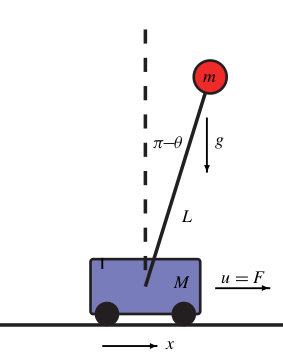
\includegraphics[width = 0.5\columnwidth]{cart-pole.png}
		\caption{Pendule inversé sur un chariot.}
		\label{fig:cart-pole}
	\end{figure}
	Soit un pendule inversé sur un chariot (voir \cref{fig:cart-pole}) dont l'équation dynamique est donné par 
	\begin{align}
		\begin{split}
			\dot{x}&=v\\
			\dot{v}&=\frac{-m^2L^2g\cos(\theta)\sin(\theta)+mL^2(mL\omega^2\sin(\theta)-\delta v)+mL^2u}{mL^2\left(M+m(1-\cos^2(\theta))\right)}\\
			\dot{\theta} &= \omega\\
			\dot{\omega} &= \frac{(m+M)mgL\sin(\theta)-mL\cos(\theta)(mL\omega^2\sin(\theta)-\delta v)-mL\cos(\theta)u}{mL^2\left(M+m(1-\cos^2(\theta))\right)}
		\end{split},
	\end{align}
	où $m$ est la masse du pendule, $M$ est la masse du chariot, $L$ est la longueur du bras, $g$ est l'accélération de la gravité,  et $\delta$ est le coéfficient de frottement sur le chariot.
	\begin{enumerate}
		\item Suivre les mêmes questions du Travail pratique encadré 1, avec $\state_{\rm f}^T = \begin{bmatrix}
			0 & 0 & 0 & 0
		\end{bmatrix}$ et $\out^T = \begin{bmatrix}
		x & \theta
		\end{bmatrix}$.
	\end{enumerate}
\end{tpe}
%\graphicspath{{Figures/}}
\chapter{Instable Feedback QP Control for Kinematic-Controlled Robots} \label{chap:instable qp}
In the previous chapter, we proposed a general formulation for the kinematic constraints \eqref{eq:second order ODI distance}--\eqref{eq:second order ODI vel} based on an adaptive-gains method.  
The conducted experiments on HRP-4 humanoid robot in closed-loop showed the performance of the proposed approach over the state-of-the-art methods. 
However, the observation of oscillations at the constraints boundary  when the constraint gains raises some questions about the stability and robustness of our formulation. For instance, oscillations are noticed at the CoM constraint boundary in  \cref{fig:CoM evolution} and which we have argued to be due to the non-modeled flexibilities at the ankles. Damped oscillations are also observed at the collision-avoidance constraint boundary in \cref{fig:different-initial-condition} and seem to correlate with high constraint gains. This fact implies that choosing high task gains will produce similar behaviors as well. These oscillations are not the desired behavior as they are generally referred to as a sign of instability. In practice, it results in discontinuous and jerky motion that can be unsafe for the robot (structural damage, actuator wearing) and the operators surrounding it. This motivates us in this chapter to investigate the sources of instability of the closed-loop QP control system.

To start our reasoning, one important remark is that the robot used for experiments is a \emph{‘kinematic-controlled robot’}, i.e., torque-controlled robots equipped with high-gains joint controllers that compute the desired joint torques $\desTau$ for the actuators (see \cref{fig:position controller}). These joint-controllers are designed by the manufacturer to track the desired joint position or velocity. Hence, if the robot behavior is instable, it means that the joint-controllers are tracking an unbounded desired input.   Since these desired inputs (joint-position or velocity) result from the double integration of the QP output $\genDesConfDDot$, it means that the QP controller generated solutions are not stable. 

%Several research works have reported similar instability phenomena of relative severity (e.g., strong sustained oscillations), see e.g.,~\cite{feng2015journalOfFieldRobotics,johnson2015journalOfFieldRobotics,dedonato2017frontiers,koolen2016ijhr}. Interestingly, it has been noted in~\cite{feng2015journalOfFieldRobotics} that the oscillations and undesired behaviors are related to the double integration of the QP output $\desConfDDot$. However, no further investigation was made to elucidate the cause. Instead, only workaround solutions have been proposed to bypass this issue. 
%Moreover,  the robots used in the above cited works rely also on joint-controllers in addition to a feedforward torque term (\cref{fig:leaky integrator QP}). The only difference with robots in \cref{fig:position controller} is the joint-controllers are numerically-implemented, whereas  they are hardware-implemented  for kinematic-controlled robots. 
 
%In~\cite{feng2015journalOfFieldRobotics}, it has been noted that the oscillations and undesired behaviors are related to the double integration of the QP output $\desConfDDot$. However, no further investigation was made to elucidate the cause.
%Furthermore, we
%Despite our method is based on an analytical solution without considering the presence of non-modeled dynamics,  However, the robustness of our formulation is questioned especially when damped oscillations  have been observed at the constraint boundary for the collision avoidance (\cref{fig:different-initial-condition}) and CoM (\cref{fig:CoM evolution}) constraints. In addition, these non-robustness behaviors may appear at the tasks as well. 

%This motivates us in this chapter to not only study the robustness of our kinematic constraints formulation, but the tasks formulation robustness as well against non-modeled dynamics. A nonrobust closed-loop control scheme leads to instability which manifests as strong oscillations and jerky motion which can be unsafe for the robot (structural damage, actuator wearing), and the people surrounding the robot.   
%\begin{figure}
%	\centering
%	\begin{tikzpicture}[auto, node distance=2cm,>=latex']
%		\node [input, name=rinput] (rinput) {};
%		\node [block, right of=u, node distance = 2.0 cm](joint controller) {Joint Controllers};
%		\node [tmp, below of= joint controller, node distance = 0.7 cm] (tmp){};
%		\node [block, right of=joint controller, node distance = 6 cm](robot) {Torque-Controlled Robot};
%		\node [tmp, right of= robot, node distance = 3.8 cm] (tmp2){};
%		\node [dotted_block, fit = (joint controller) (robot) (robot) (tmp)] (pos controller) {};		
%		\node at (pos controller.north) [above, inner sep=1.5mm] {Kinematic-Controlled Robot};
%		%	\draw [->] (u) -- node{$\jointCrtlIn$}(xd dynamics);
%		\draw [->] (rinput) -- node[pos=0.3]{$
%			\left[\desConf \ \desConfDot\right]
%			$}(joint controller);%node{$\desConfDDot$}(InvDyn);
%		%\draw [->] (QP.north) |- node{$\desConfDDot$}(integrator.west);
%		\draw [->] (joint controller) -- node{$\desTau$}(robot);
%		\draw [->] (robot) -- node[pos=0.65]{$
%			\left[\actConf \  \actConfDot\right]
%			$}(tmp2);
%		\draw [-] ([xshift=-35pt]tmp2) |- (tmp);
%		\draw [->] (tmp) -- (joint controller.south);
%		%	 			\draw [->] (sum) -- node{}(robot);
%		%	 			\draw [->] (integrator.east) -- node{$
%			%	 				\left[\desConf \ \desConfDot\right]
%			%	 				$}(feedback.west);
%		%	 			\draw [-] (robot) -- node{$
%			%	 				\left[\actConf \  \actConfDot\right]
%			%	 				$}(x2);
%		%	 			\draw [-] (x2) |- (aux);
%		%	 			\draw [->] (x2) -- (x3);
%		%	 			\draw [->] (aux) -- node{}(QP.south);
%		%	 			%	\draw [->] (alphad2) -- node{}([xshift=-10pt]InvDyn.south);
%		%	 			\draw [->] (alphad) -- node{}([xshift=-0pt]InvDyn.south);
%		%	 			%	\draw [-] (xd) |- node{}(alphad3);
%		%	 			%	\draw [->] (alphad3) -- node{}([xshift=10pt]integrator.south);
%		%	 			\draw [-] (x2) |- (xBis);
%		%	 			\draw [->] (xBis) -- (integrator.north);
%		%	 			\draw [-] (feedback.south) -- (sumTmp);
%		%	 			\draw [->] (sumTmp) -| (sum.north);
%		%	 			\draw [->] ([xshift=2pt]alphaD) |-  (integrator.west);
%		%	\draw [->] (alphaD) |- node{$\desConfDDot$}(integrator.west);
%		%	\draw [->] (disturbance) --node{$\jointDisturbIn$} (x dynamics.north);
%	\end{tikzpicture}		
%	\caption{Illustrative block scheme of a kinematic-controlled robot (dotted) which, for a matter of space, denotes ‘Robot’ block in \cref{fig:QP scheme for kinematic-control robots}-\ref{fig:whole control scheme}.}
%	\label{fig:position controller}
%\end{figure}

In this chapter, we  study the effect of the joint-controllers on the stability of the closed-loop system containing a QP controller and kinematic-controlled robot. Instead of considering the robot as a multi-DoF system, we only focus on a case-study:  1-DoF  system (an actuator servoed by a PD-controller). In \cref{sec-chap2:1-DoF robot}, we  introduce more in detail the kinematic-controlled robots and explain why the 1-DoF case-study is sufficient for the stability study. Then, we  model the dynamics of a DC motor servoed with a PD-controller. In \cref{sec-chap2:QP stability investigation}, we investigate the stability of a QP controller in cascade with the 1-DoF system following two closed-loop control schemes (\cref{fig:QP scheme for kinematic-control robots}), and show the pros and cons of each. Finally, we propose an approach that ensures the stability while reactively counterbalancing external disturbances.    
%Although it is a simple case but it is sufficient to understand 

%In our study, we will focus particularly on ‘kinematic-controlled robots’ which is a general term that encompasses the robots that are controlled by sending either the desired joint position (position-controlled) or the desired joint velocity (velocity-controlled). These robots are equipped with high-gains joint controllers that compute the desired joint torques $\desTau$ for the actuators (see \cref{fig:position controller}). Stiff kinematic-controlled robots are widely used in robotics and automation industry as the knowledge of the robot's dynamics is not required~\cite{garcia2004iros,rossi2014iros,zanchettin2017elsevier,singletary2022csl,polverini2017ral,suarez2018sciRob,lim2016journalOfFieldRobotics}. Nevertheless, their joint dynamics (joint controllers + actuators) are generally not known as they depend on the joint controller gains (fixed by the manufacturer not intended to be modified by the operator in almost all robots) and the actuators electro-mechanical constants. Consequently, the non-modeled joint-dynamics rise as the main factor of non-robustness of the closed-loop QP controller. Other non-modeled dynamics can be considered like sensor noises, and flexibilities especially for humanoid robots which often contains soft materials at the ankles to lower the walking impacts on the whole structure.  

%In this chapter, we will consider a simple example of a 1-DoF position-controlled robot controlled by a QP. This simple case-study will enables us to provide answers for the following questions (i) what leads the closed-loop QP control scheme to be non-robust and thereby instable; (ii) how can we ensure robustness of the closed-loop QP control. 
%First we will 


%\begin{itemize}
%	%	\item The gains adaptation method is based on an analytical solution without considering the presence of non-modeled dynamics
%	%	\item In the next section, we will particularly  focus on the case of kinematically controlled (position-controlled) robots which joint-dynamics is not modeled in addition to other factors like flexibilities and sensor noise 
%	%\item {\color{red} Since the analytical solution cannot be used anymore, we propose a robust constraint formulation based on Control Barrier Function theory }
%\end{itemize} 
%\section{State-of-the-Art}\label{sec-chap2:sota chap2}
%%QP control has been successfully applied to complex robots and scenarios~\cite{escande2014ijrr,salini2011icra,herzog2016autonomousRobot,kuindersma2016autonomousRobot,feng2014humanoids,nava2020ral,hamed2020ral,englsberger2015tro,klemm2020ral,basso2020ifac,reher2021arxiv-tro}. 
%%Yet, 
%Several research works reported instability phenomena of relative severity (e.g., strong sustained oscillations), see e.g.,~\cite{feng2015journalOfFieldRobotics,johnson2015journalOfFieldRobotics,dedonato2017frontiers,koolen2016ijhr}. Interestingly, the common factor in each reported shortcoming is that the joint torque control relies on joint-position and/or velocity feedback terms in addition to $\desTau$ (\cref{fig:leaky integrator QP}). In~\cite{feng2015journalOfFieldRobotics}, it has been noted that the oscillations and undesired behaviors are related to the double integration of the QP output $\desConfDDot$. However, no further investigation was made to elucidate the cause.
%
%Workaround solutions have been proposed to mitigate this issue. These palliative methods can be sorted into two categories: (i) \emph{low-level approaches} that act at the joint-level to prevent $\desConfDDot$ double integration from diverging; typically by implementing a leaky integrator~\cite{hopkins2015icra}; and (ii) \emph{high-level approaches}  where the QP formulation is substantially modified at the expense of a complex control-architecture~\cite{feng2014humanoids,feng2015journalOfFieldRobotics}, or by accounting for the joint feedback terms in the QP to adapt their gains~\cite{lee2022frontiersRobS} or for constraints feasibility concerns~\cite{cisneros2018iros}. Other approaches reported that lowering the task gains helps mitigating the instability~\cite{koolen2016ijhr,johnson2015journalOfFieldRobotics} which highlights the fact that task gains are also an interfering factor. Similar observation is made in~\cite{djeha2020ral,singletary2022csl} concerning the gains of the safety-constraint formulation. 
%
%The closed-loop task-space QP controller combined with a joint low-level kinematic-controlled robot,~\cref{fig:QP scheme for kinematic-control robots}\subref{subfig:feedback QP}, is also prone to previously described instability shortcomings.  
%The latter have been unnoticed in some control implementations that operate in feedforward (\cref{fig:QP scheme for kinematic-control robots}\subref{subfig:feedforward QP}). This leads to a decoupled control (similar to~\cite{feng2015journalOfFieldRobotics}), delegating the control accuracy to the joint controllers~\cite{bouyarmane2018tac,zanchettin2017elsevier,polverini2017iros_a}. In such cases, frequent initializations of the controller are needed to lower the discrepancy between real and control-model states due to non-modeled flexibilities or external disturbance. 

%\begin{figure}%[t!]
%	\centering
%	\begin{tikzpicture}[auto, node distance=2cm,>=latex']
%		\node [input, name=rinput] (rinput) {};
%		\node [tmp, right of=rinput, node distance = 0.0 cm](u){};
%		\node [block, right of=u, node distance = 0 cm](QP) {QP};
%		\node [tmp, right of=QP, node distance = 1cm] (alphaD){};
%		
%		%	\node [tmp, above of=InvDyn, node distance = 1. cm] (tmp1){};
%		\node [block, right of = QP, node distance = 3 cm] (integrator) {Double Integrator};
%		\node [sum, right of = integrator, node distance = 3.5 cm] (sum2){};
%		%			 			\node [block, left of = tmp1, node distance = 0.0 cm,xshift=-2pt] (integrator) {Leaky Integrator};
%		\node [block, right of = sum2, node distance = 2.2 cm] (feedback) {Joint Controllers};
%		
%		\node [tmp, below of=sum2, node distance = 1 cm] (xFeedback){};
%		\node [tmp, below of=QP, node distance = 1.0 cm] (xQP){};
%		\node [sum, right of = feedback, node distance = 2.2 cm] (sum){};
%		\node [tmp, above of=sum, node distance = 1.1 cm](InvDyn) {};
%		\node [block, right of=sum, node distance = 1.2 cm](robot) {Robot};		
%		\node [tmp, right of=robot, node distance = 0.8 cm](x){};
%		\node [tmp, right of=x, node distance = 0.7 cm](x2){};
%		
%		
%		%	\draw [->] (u) -- node{$\jointCrtlIn$}(xd dynamics);
%		
%		\draw [-] ([yshift=0pt]QP.north) |- node[above,pos=0.54]{$\desTau$}(InvDyn);
%		%\draw [->] (QP.north) |- node{$\desConfDDot$}(integrator.west);
%		\draw [->] (InvDyn) -- node[above,pos=0.9]{}(sum);
%		%		\draw [-] ([yshift=+2.5pt]QP.east) -| node[above,pos=0.3]{}([xshift=-50pt,yshift=2.5pt]InvDyn);
%		%		\draw [-] ([yshift=+2.5pt]QP.east) -| node[above,pos=0.3]{}([xshift=-50pt,yshift=2.5pt]InvDyn);
%		%		\draw [->] ([xshift=-50pt,yshift=2.5pt]InvDyn) |- node[above,pos=0.7]{$\desConfDDot$}(integrator.west);
%		\draw [->] (QP.east) |- node[above, pos = 0.8]{$\genDesConfDDot$}(integrator.west);
%		\draw [->] (sum) -- node{}(robot);
%		\draw [->] (integrator.east) -- node[above, pos = 0.5]{$
%			\left[\desConf \ \desConfDot\right]
%			$}(sum2);
%		\draw [->] (sum2.east) -- node{}(feedback);
%		\draw [->] (feedback.east) -- node{}(sum);
%		\draw [-] (robot) -- node[above, pos = 1]{$
%			\left[\actConf \  \actConfDot\right]
%			$}(x2);
%		\draw [-] ([xshift = 0pt]x2) |- (xFeedback);
%		\draw [->] (xFeedback) -- node[pos = 0.8]{$-$}(sum2);
%		%	\draw [->] (x2) -- (x3);
%		\draw [-] (xFeedback) -- node{}(xQP);
%		\draw [->] (xQP) -- node{}(QP);
%		%	\draw [->] (alphad2) -- node{}([xshift=-10pt]InvDyn.south);
%		%\draw [->] (alphad) -- node{}([xshift=-0pt]InvDyn.south);
%		%	\draw [-] (xd) |- node{}(alphad3);
%		%	\draw [->] (alphad3) -- node{}([xshift=10pt]integrator.south);
%		%	\draw [-] (x2) |- (xBis);
%		%	\draw [->] ([xshift = 4pt]x2) |- (feedback.east);
%		%			 			\draw [-] (xBis) -- (xBisInt);
%		%			 			\draw [->] (xBisInt) -- (integrator.north);
%		%	\draw [-] (feedback.south) -- (sumTmp);
%		%\draw [->] (sumTmp) -| node[pos=1, above, xshift =-5pt]{$+$}(sum.north);
%		
%		%	\draw [->] ([xshift=2pt]alphaD) |-  (integrator.west);
%		%	\draw [->] ([yshift=5pt]QP.east) |- (integrator.west);
%		%	\draw [->] (alphaD) |- node{$\desConfDDot$}(integrator.west);
%		%	\draw [->] (disturbance) --node{$\jointDisturbIn$} (x dynamics.north);
%	\end{tikzpicture}
%	
%	\caption{QP control scheme for torque-controlled robots with additional joint feedback. ‘Robot’ is torque-controlled.}
%	\label{fig:leaky integrator QP}
%\end{figure}
\begin{figure}[t!]
	\centering
	\subfloat[]{
		\begin{tikzpicture}[auto, node distance=2cm,>=latex']
			\node [input, name=rinput] (rinput) {};
			\node [tmp, right of=rinput, node distance = 0.5 cm](u){};
			\node [block, right of=u, node distance = 0 cm](QP) {QP};
			\node [tmp, right of=QP, node distance = 0.5 cm] (alphaD){};
			\node [block, right of=alphaD, node distance = 3 cm](integrator) {Double Integrator};
			\node [tmp, right of=integrator, node distance = 2.2 cm] (xd){};
			\node [block, right of=xd, node distance = 2 cm](robot) {Robot};
			\node [tmp, right of=robot, node distance = 1 cm](x){};
			\node [tmp, right of=x, node distance = 0.7 cm](x2){};
			\node [tmp, below of = QP, node distance = 0.7cm] (aux){};
			%	\draw [->] (u) -- node{$\jointCrtlIn$}(xd dynamics);
			\draw [->] (QP) -- node{$\desConfDDot$}(integrator);
			\draw [->] (integrator) -- node{$
				\left[\desConf \ \desConfDot\right]
				$}(robot);
			\draw [->] (robot) -- node{$
				\left[\actConf \  \actConfDot\right]
				$}(x2);
			\draw [-] (x) |- (aux);
			\draw [->] (aux) -- node{}(QP.south);	
			%	\draw [->] (disturbance) --node{$\jointDisturbIn$} (x dynamics.north);
		\end{tikzpicture}
		\label{subfig:feedback QP}}
	\hfil
	\subfloat[]{
		\begin{tikzpicture}[auto, node distance=2cm,>=latex']
			\node [input, name=rinput] (rinput) {};
			\node [tmp, right of=rinput, node distance = 0.5 cm](u){};
			\node [block, right of=u, node distance = 0 cm](QP) {QP};
			\node [tmp, right of=QP, node distance = 0.5 cm] (alphaD){};
			\node [block, right of=alphaD, node distance = 3 cm](integrator) {Double Integrator};
			\node [tmp, right of=integrator, node distance = 2.2 cm] (xd){};
			\node [block, right of=xd, node distance = 2 cm](robot) {Robot};
			\node [tmp, right of=robot, node distance = 1 cm](x) {};
			\node [tmp, right of=x, node distance = 0.7 cm](x2){};
			%	\node [tmp, right of=robt, node distance = 2 cm](x){};
			\node [tmp, below of = QP, node distance = 0.7cm] (aux){};
			%	\draw [->] (u) -- node{$\jointCrtlIn$}(xd dynamics);
			\draw [->] (QP) -- node{$\desConfDDot$}(integrator);
			\draw [->] (integrator) -- node{$
				\left[\desConf \  \desConfDot\right]
				$}(robot);
			\draw [-] (xd) |- (aux);
			\draw [->] (aux) -- node{}(QP.south);
			\draw [->] (robot) -- node{$
				\left[\actConf \  \actConfDot\right]
				$}(x2);
			%	\draw [->] (disturbance) --node{$\jointDisturbIn$} (x dynamics.north);
		\end{tikzpicture}
		\label{subfig:feedforward QP}}
%	\hfil
%	\subfloat[]{
%		\begin{tikzpicture}[auto, node distance=2cm,>=latex']
%			%	 			\node [input, name=rinput] (rinput) {};
%			%	 			\node [tmp, right of=rinput, node distance = 0.5 cm](u){};
%			\node [block, draw = black, ](QP) {QP};
%			\node [tmp, right of=QP, node distance = 0.5 cm] (alphaD){};
%			\node [block, right of=alphaD, node distance = 3 cm, draw = black, ](integrator) {Double Integrator};
%			\node [tmp, right of=integrator, node distance = 2.2 cm] (xd){};
%			\node [block, right of=xd, node distance = 2 cm, draw = black, ](robot) {Robot};
%			\node [tmp, right of=robot, node distance = 1 cm](x){};
%			\node [tmp, right of=x, node distance = 0.7 cm](x2){};
%			\node [tmp, below of = QP, node distance = 0.7cm] (aux){};
%			\node [tmp, below of = QP, node distance = 0.57cm] (aux2){};
%			%	\draw [->] (u) -- node{$\jointCrtlIn$}(xd dynamics);
%			\draw [->, color=black, ] (QP) -- node{$\desConfDDot$}(integrator);
%			\draw [->, color=black, ] (integrator) -- node{$
%				\left[\desConf \  \desConfDot\right]
%				$}(robot);
%			\draw [->, color=black, ] (robot) -- node{$
%				\left[\actConf \  \actConfDot\right]
%				$}(x2);
%			\draw [-, color=black, ] (x) |- ([xshift=-5pt]aux);
%			\draw [-, color=black, ] (xd) |- ([xshift=5pt]aux2);
%			%\draw [-] (aux) -- node{}(rinput);	
%			\draw [->, color=black, ] ([xshift=-5pt]aux) -- node{}([xshift=-5pt]QP.south);
%			\draw [->, color=black, ] ([xshift=5pt]aux2) --([xshift=5pt]QP.south);
%			%	\draw [->] (disturbance) --node{$\jointDisturbIn$} (x dynamics.north);
%		\end{tikzpicture}
%		\label{subfig:our QP}}		
	\caption{Different closed-loop QP control schemes for kinematic-controlled robots.
		%~\subref{subfig:leaky integrator QP} Leaky integrator QP in~\cite{hopkins2015icra}.
		~\subref{subfig:feedback QP} Feedback QP.
		~\subref{subfig:feedforward QP} Feedforward QP.}
		%~\subref{subfig:our QP} Proposed robust QP. }
	\label{fig:QP scheme for kinematic-control robots}
\end{figure}


\section{Kinematically-Controlled Robots}\label{sec-chap2:1-DoF robot}
\begin{figure}
	\centering	
	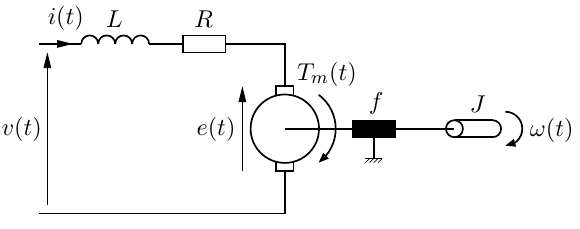
\includegraphics[width=0.6\columnwidth]{DCC model.pdf}
	\caption{DC motor model}
	\label{fig:DCmodel}
\end{figure}
\begin{table}
	\centering
	\begin{tabular}{|c|c|}
		\hline 
		& Parameters \\
		\hline
		Electrical & 
		\begin{tabular}{@{}c@{}}
			$v(t)$: Voltage input (V) \\
			$i(t)$: Current (A) \\ 
			$e(t)$: Electro-Motive Force (EMF) (V) \\
			$\tau_{\rm l}(t)$: Load torque (Nm) \\
			$\tau_{\rm m}(t)$: Motor torque (Nm) \\
			$L$: Inductance (H) \\ 
			$R$: Resistance ($\varOmega$) \\ 
			$K$: Torque and EMF constant (V.s.rad$^{-1}$)
		\end{tabular}\\
		\hline
		Mechanical & 
		\begin{tabular}{@{}c@{}}
			$\omega_m(t)$: Motor-side angular velocity\\
			$\omega(t)$: Link-side angular velocity\\
			$J$: Rotor inertia ($Kg.m^2$) \\ 
			$f$: Friction coef. ($N.m.s.rad^{-1}$) \\ 
			$N$: Gear ratio\end{tabular} \\
		\hline
	\end{tabular}
	\caption{Specification of the electrical and mechanical parameters.}
	\label{tab:DC motor paramters}
\end{table}
Stiff kinematic-controlled robots are widely used in robotics and automation industry as the knowledge of the robot's dynamics is not required~\cite{garcia2004iros,rossi2014iros,zanchettin2017elsevier,singletary2022csl,polverini2017ral,suarez2018sciRob,lim2016journalOfFieldRobotics,singletary2022csl}. Controlling a kinematic-controlled robot rely on a simple control strategy which consists in considering the robot with $n$-actuated DoF as a system of $n$ independent joints. Each joint is actuated with a motor servoed by a joint-controller, resulting in a Single-Input/Single-Output (SISO) system. The joint-level servoing can performed either in position (i.e., regulate the error between the desired joint position $\desConf$ and the actual joint position $\actConf$ to zero) or in velocity (i.e., regulate the error between the desired joint velocity $\desConfDot$ and the actual joint velocity $\actConfDot$ to zero)~\cite{albu-schaffer2007industrialRobot,albu-shaffer2007ijrr,mistry2008humanoids,iskandar2020iros,lim2016journalOfFieldRobotics,lim2017journalOfFieldRobotics}. %(\cref{fig:position controller}). 

The most known and documented joint-controller is the position Proportional-Derivative (PD) joint-controller~\cite{spong2020bookRobotModeling,siciliano2010robotics}
\begin{align}
	\massMat(\genActConf) \genActConfDDot + \nnLinTorqueMat(\genActConf,\genActConfDot)\genActConfDot + \gravity&= \selectMat\bm{\tau}_{\rm PD}, \\
	\bm{\tau}_{\rm PD} &= -\mathbf{P}(\actConf - \desConf) - \mathbf{D}\actConfDot
\end{align}
where $\mathbf{P}$ and $\mathbf{D}$ are diagonal positive gains matrices to ensure decoupled joint-torque computation. 
 The coupling effects between the joints (mass, Coriolis-centrifugal and gravity torques, etc.) are perceived as an external disturbance torque input. The latter can be counterbalanced by a feedforward torque term computed from EoM~\eqref{eq-chap0:equation of motion} as shown in \cref{fig:leaky integrator QP} 
 \begin{align}
 	\massMat(\genActConf) \genActConfDDot + \nnLinTorqueMat(\genActConf,\genActConfDot)\genActConfDot +\gravity&= \selectMat\left(\bm{\tau}_{\rm PD} + \bm{\tau}_{\rm d}\right). 
% 	\\
% 	\bm{\tau}_{\rm PD} &= -\mathbf{P}(\actConf - \desConf) - \mathbf{D}\actConfDot
 \end{align}
 In fact, this approach is extensively used for torque-controlled robots to overcome the joint non-modeled static friction~\cite{hopkins2015icra,hopkins2015iros,cisneros2018iros,kuindersma2016autonomousRobot,koolen2016ijhr,hopkins2015icra}.   

Generally, the motors have different sizes and characteristics depending on their placement and role on the robot's whole-body (the more load the actuator is intended to receive, the larger and more powerful is). The joint-controller gains are correspondingly tuned by the manufacturer to ensure good tracking (large bandwidth) and disturbance attenuation performances. This is the main reason why the joint-controllers usually have high gains. 
Since the joints are controlled independently (SISO assumption), we focus the stability study in this chapter on a single actuator controlled by QP. Namely, the study conducted for one joint applies straightforwardly to the others.  
We model a DC motor servoed by a PD controller. Next, we study the stability of this inner system when an outer QP controller controls it. 

\subsection{Case-Study: 1-DoF Actuator}
A DC motor is modeled by electrical and mechanical components as in \cref{fig:DCmodel}. The electrical and mechanical equations describing the system are the following:
\begin{align}\label{eq:DCmodelEquations}
	\begin{split}
		v(t) &=  Ri(t) + e(t)\\
		e(t) &= K\omega_m(t)\\
		\tau_{\rm m}(t) &=Ki(t) \\
		\tau_{\rm m}&=J\frac{d\omega_m(t)}{dt} + f\omega_m(t) + \frac{\tau_{\rm l}(t)}{N}\\
		\omega_{\rm m}(t) &= N\omega(t)\\
		\omega(t) & = \dot{\hat{q}}(t)
	\end{split}
\end{align}
All the parameters are defined in \cref{tab:DC motor paramters} 
%where $\omega_m$ and $\omega$ are the articular velocities at the motor and link-side respectively, $v(t)$ is the voltage, $i(t)$ denotes the current, $e(t)$ is the electro-mechanical force, $T_m(t)$ is the motor torque, and $T_l(t)$ is the external load torque. The superscript $ ^{j\in\mathbb{N}}$ denotes an actuator$^j$ on the robot. 
By manipulating equations~\eqref{eq:DCmodelEquations}, we obtain the following link-side electro-mechanical equation:
\begin{align}\label{eq:electroMecanicEquation}
	\begin{split}
		v(t) &= \frac{JNR}{K}\frac{d\omega(t)}{dt} + \frac{N(Rf + K^2)}{K}\omega(t) + GT_l(t)\\
		G &= \frac{R}{KN}
	\end{split}
\end{align} 
Considering $f\approx0$, and non-loaded case $\tau_{\rm l}=0$, the transfer function between the voltage $v$ and joint position $\hat{q}$ is :
\begin{align}\label{eq:DCmodelTransferFunction}
	\begin{split}
		R(s)=\frac{v(s)}{\hat{q}(s)}& = \frac{a}{s(s + b)},\\
		a & = \frac{K}{NRJ},\\
		b & = \frac{ K^2}{RJ}.
	\end{split}
\end{align}
The system~\eqref{eq:DCmodelTransferFunction} is servoed by a PD controller as shown in Figure~\ref{fig:lowLevelSystem}. Considering the PD controller transfer function $C(s) = P + Ds$ with $P$ and $D$ are the gains, the joint-level transfer function between the desired joint position $\hat{q}_{\rm d}$ and actual joint position $\hat{q}$ is: 
\begin{align}\label{eq:qd-q TransferFunction}
	\begin{split}	
		F(s)&=\frac{\hat{q}(s)}{\hat{q}_{\rm d}(s)}=\frac{C(s)R(s)}{1 + C(s)R(s)} = \frac{\delta s + \gamma}{s^2 + \beta s + \gamma},\\
		\delta &= aD,\\
		\gamma &= aP,\\
		\beta &= b + aD.\\
	\end{split}
\end{align}
\begin{figure}
	\centering	
	\includegraphics[width=0.75\columnwidth]{LowLevelSystem-relabled}
	\caption{Joint-dynamics with its inputs and outputs.}
	\label{fig:lowLevelSystem}
\end{figure}
Now, let us consider $\tau_{\rm l}(t)\neq0$. This leads to the following expression:
\begin{align}\label{eq:tau-q TransferFunction}
	\begin{split}
		\hat{q}(s) &= F(s)\hat{q}_{\rm d}(s) + H(s)\tau_{\rm l}(s),\\
		H(s) &=\frac{GR(s)}{1 + C(s)R(s)} = \frac{aG}{s^2 + \beta s + \gamma }.
	\end{split}
\end{align}
%{\color{red}Later, we will use~\eqref{eq:tau-q TransferFunction} to explain the effect of the torque load on the system response. Hereafter, let us consider it null.}
From \cref{eq:tau-q TransferFunction}, it can be seen that the higher $P$, the more the steady-state disturbance effect ($\frac{G}{P}$) is attenuated. Furthermore, $P$ and $D$ are tuned (by the manufacturer) such that the systems $F(s)$ and $H(s)$ poles are stable.  
Giving~\cref{eq:qd-q TransferFunction} and \cref{eq:tau-q TransferFunction}, we can write the following  differential equation
%\begin{equation}\label{eq:lowLevelDiffEquation}
%	\delta\dot{\hat{q}}_{\rm d} + \gamma \hat{q}_{\rm d} = \ddot{\hat{q}} + \beta \dot{\hat{q}} + \gamma \hat{q}
%\end{equation}
\begin{equation}\label{eq:lowLevelDiffEquation}
	\ddot{\hat{q}} =   - \beta \dot{\hat{q}} - \gamma \hat{q} + \delta\dot{\hat{q}}_{\rm d} + \gamma \hat{q}_{\rm d} + aG \tau_{\rm l}
\end{equation}
\cref{eq:lowLevelDiffEquation} describes the \emph{joint-dynamics} and which is seen as the inner control loop. Next, we control this inner loop with a QP controller in closed-loop.
\subsection{QP Controller and Joint-Dynamics Model in Cascade}
For simplicity, we consider first an unconstrained QP controller. Given a target reference $\hat{q}_{\rm ref}$, the role of QP is to generate $\hat{q}_{\rm d}$ and forward it to the joint-dynamics such that both $\hat{q}_{\rm d}$ and $\hat{q}$ converge to $\hat{q}_{\rm ref}$. 
Let us define $x$ as 
\begin{equation}
	x = \begin{bmatrix}
		\hat{q} - \hat{q}_{\rm ref} \\ 
		\dot{\hat{q}}  \\
		\hat{q}_{\rm d} - \hat{q}_{\rm ref} \\
		\dot{\hat{q}}_{\rm d}  
	\end{bmatrix}\inR^4.
\end{equation}
 Then, the differential equation~\eqref{eq:lowLevelDiffEquation} can be written in the state-space form 
\begin{equation}\label{eq:lowLevelSSEquation}
	\dot{x} = \begin{bmatrix}
		0 & 1 & 0 & 0 \\
		-\gamma & -\beta & \gamma & \delta \\ 
		0 & 0 & 0 & 1 \\ 
		0 & 0 & 0 & 0 
	\end{bmatrix}x + 
	\begin{bmatrix}
		0 \\ 0 \\ 0 \\ 1
	\end{bmatrix}\ddot{\hat{q}}_{\rm d} + 
	\begin{bmatrix}
		0 \\ aG \\ 0 \\ 0
	\end{bmatrix}\tau_{\rm l}.
\end{equation}
Now, the unconstrained QP formulated for 1-DoF system is given as 
\begin{equation}\label{eq:task feedback 1DoF}
	\ddot{\hat{q}}_{\rm d} = - \mathbf{K}x, 
\end{equation}
where $\mathbf{K}\inR^{1\times 4}$ is the task feedback gain-matrix. In the next section, we see how we can formulate the gain matrix $\mathbf{K}$ and the subsequent stability implications.
\section{QP Closed-Loop Stability Study}\label{sec-chap2:QP stability investigation}
 The task feedback~\eqref{eq:task feedback 1DoF} can be designed in several ways depending on the closed-loop control schemes: either in feedforward \cref{fig:QP scheme for kinematic-control robots}\subref{subfig:feedforward QP}, or in feedback \cref{fig:QP scheme for kinematic-control robots}\subref{subfig:feedback QP}. In what follows, we study the closed-loop stability of both control schemes. 
\subsection{Feedforward Control Scheme}\label{subsec-chap2:feedforward control scheme}
Considering the control scheme \cref{fig:QP scheme for kinematic-control robots}\subref{subfig:feedforward QP}, the task feedback~\eqref{eq:task feedback 1DoF} can formulated as 
\begin{equation}\label{eq:feedforward task feedback 1DoF}
	\ddot{\hat{q}}_{\rm d} = - \begin{bmatrix}
		0 & 0 & K_{\rm s} & K_{\rm d} 
	\end{bmatrix}x,  
\end{equation}
where $K_{\rm s}, K_{\rm d} >0 $ are the stiffness and damping gains, respectively. 
Replacing \cref{eq:feedforward task feedback 1DoF} in \cref{eq:lowLevelSSEquation}, we get the closed-loop form
\begin{equation}\label{eq:feedforward 1DoF closedLoop}
	\dot{x} = \mathbf{A}^{\rm FF}x + \begin{bmatrix}
		0 \\ aG \\ 0 \\ 0
	\end{bmatrix}\tau_{\rm l}, \ \mathbf{A}^{\rm FF} = 
	\begin{bmatrix}
		0 & 1 & 0 & 0 \\
		-\gamma & -\beta & \gamma & \delta \\ 
		0 & 0 & 0 & 1 \\ 
		0 & 0 & -K_{\rm s} & -K_{\rm d} 
	\end{bmatrix}.
\end{equation}
The stability of closed-loop system~\eqref{eq:feedforward 1DoF closedLoop} depends on the matrix $\mathbf{A}^{\rm FF}$. One necessary and sufficient condition for stability is that $\mathbf{A}^{\rm FF}$ is Hurwitz~\cite{khalil2002NonLinearSystems}. This can be easily verified by computing $\mathbf{A}^{\rm FF}$ eigenvalues $\bm{\lambda}\left(\mathbf{A}^{\rm FF}\right)$ and checking their real part is strictly negative. 

The form of $\mathbf{A}^{\rm FF}$ enables us to have a closed-form of the eigenvalues such that\footnote{The eigenvalues closed-form has been obtained using the symbolic computation software Maple.} 
\begin{equation}\label{eq:feedforward eigenvalues}
	\bm{\lambda}\left(\mathbf{A}^{\rm FF}\right) = \frac{1}{2}\begin{bmatrix}
		-\beta + \sqrt{\beta^2 - 4\gamma} \\
		-\beta - \sqrt{\beta^2 - 4\gamma} \\
		-K_{\rm d}  + \sqrt{K_{\rm d}^2 - 4K_{\rm s} } \\
		-K_{\rm d}  - \sqrt{K_{\rm d}^2 - 4K_{\rm s} }    
	\end{bmatrix}
\end{equation}
\begin{table}
	\centering		
	\begin{tabular}{|c||c|c|}\hline
		&  1   &  2 \\\hline
		$\beta$&$158.5073$ &$173.5712$ \\\hline
		$\gamma$&$376.5977$ &$2380.6356$ \\\hline
		$\delta$&$2.8245$  &$17.8884$ \\	\hline
		%$K_{\rm s}$&$2.8245$    &$2.0713$\\\hline
		%$K_{\rm d}$&$4.7034$    &$0.9407$\\\hline
		$aG$&$4.7034$    &$4.7034$\\\hline
	\end{tabular}
\caption{Parameters used for system~\eqref{eq:lowLevelSSEquation} numerical simulations. The parameters in column 2 are obtained by choosing higher $P$ and $D$ gains than those in column 1.}
\label{tab:parameters}
\end{table}
From~\cref{eq:feedforward eigenvalues}, the eigenvalues $\bm{\lambda}\left(\mathbf{A}^{\rm FF}\right)$ are stable and decoupled. Namely,  the eigenvalues relative to the joint-dynamics are decoupled from those relative to the task gains. Hence, the closed-loop system~\eqref{eq:feedforward 1DoF closedLoop} is systematically stable whatever the joint-dynamics and whatever the task gains. However, if $\tau_{\rm l}\neq 0 $ then $\hat{q}$ does not converge strictly to $\hat{q}_{\rm ref}$ (\cref{fig:openloop 1dof simulation}). This is expected since the task feedback~\eqref{eq:feedforward task feedback 1DoF} does not account for the actuator state ($\hat{q}, \dot{\hat{q}}$).

\begin{figure}[htp!]
	\centering
	\subfloat[]{
	\includegraphics[width=0.47\columnwidth]{Stable5-Perturbation}
	\label{subfig:sys1-openloop5-perturbation}
	}
	\hfil
	\subfloat[]{
		\includegraphics[width=0.47\columnwidth]{Stable30-Perturbation}
		\label{subfig:sys1-openloop30-perturbation}
	}
	\hfil
	\subfloat[]{
		\includegraphics[width=0.47\columnwidth]{system2-stable5-perturbationZ}
		\label{subfig:sys2-openloop5-perturbation}
	}
	\hfil
	\subfloat[]{
		\includegraphics[width=0.47\columnwidth]{system2-stable30-perturbationZ}
		\label{subfig:sys2-openloop30-perturbation}
	}
	\caption{Closed-loop response of system~\eqref{eq:feedforward 1DoF closedLoop}. External torque disturbance $\tau_{\rm l} = 3$~Nm is applied at $t=6$~s. The system parameters are taken from columns 1 (top) and 2 (bottom) in  \cref{tab:parameters}. \subref{subfig:sys1-openloop5-perturbation}--\subref{subfig:sys2-openloop5-perturbation} $K_{\rm s} = 5$, $K_{\rm d} = 2\sqrt{K_{\rm s}}$. \subref{subfig:sys1-openloop30-perturbation}--\subref{subfig:sys2-openloop30-perturbation} $K_{\rm s} = 30$, $K_{\rm d} = 2\sqrt{K_{\rm s}}$.}
	\label{fig:openloop 1dof simulation}
\end{figure}
\subsection{Feedback Control Scheme}\label{subsec-chap2:feedback control scheme}
Considering the feedback closed-loop control scheme in \cref{fig:QP scheme for kinematic-control robots}\subref{subfig:feedback QP}, the task feedback~\eqref{eq:task feedback 1DoF} can formulated as 
\begin{equation}\label{eq:feedback task feedback 1DoF}
	\ddot{\hat{q}}_{\rm d} = - \begin{bmatrix}
		 K_{\rm s} & K_{\rm d} &0 & 0 
	\end{bmatrix}x,  
\end{equation}
Replacing \cref{eq:feedback task feedback 1DoF} in \cref{eq:lowLevelSSEquation}, we get the closed-loop form
\begin{equation}\label{eq:feedback 1DoF closedLoop}
	\dot{x} = \mathbf{A}^{\rm FB}x + \begin{bmatrix}
		0 \\ aG \\ 0 \\ 0
	\end{bmatrix}\tau_{\rm l}, \ \mathbf{A}^{\rm FB} = 
	\begin{bmatrix}
		0 & 1 & 0 & 0 \\
		-\gamma & -\beta & \gamma & \delta \\ 
		0 & 0 & 0 & 1 \\ 
		-K_{\rm s} & -K_{\rm d} & 	0 & 0 
	\end{bmatrix}.
\end{equation}
As for the system~\eqref{eq:feedforward 1DoF closedLoop}, the closed-loop system~\eqref{eq:feedback 1DoF closedLoop} stability depends on the eigenvalues of $\mathbf{A}^{\rm FB}$. However, and conversely to system~\eqref{eq:feedback task feedback 1DoF}, $\mathbf{A}^{\rm FB}$ eigenvalues do not have a simple form as in \cref{eq:feedforward eigenvalues}\footnote{The computation with Maple provided very long and complicated formulas where the task gains and joint-dynamics parameters are coupled.}. Alternatively, running the same simulations as in \cref{subsec-chap2:feedforward control scheme} shows that, in this case, the closed-loop stability is not systematically guaranteed as shown in \cref{fig:closedloop 1dof simulation}.    
\begin{figure}[htp!]
	\centering
	\subfloat[]{
		\includegraphics[width=0.47\columnwidth]{system1-CL5-perturbation}
		\label{subfig:sys1-CL5-perturbation}
	}
	\hfil
	\subfloat[]{
		\includegraphics[width=0.47\columnwidth]{system1-CL30-perturbation}
		\label{subfig:sys1-CL30-perturbation}
	}
	\hfil
	\subfloat[]{
		\includegraphics[width=0.47\columnwidth]{system2-CL5-perturbation}
		\label{subfig:sys2-CL5-perturbation}
	}
	\hfil
	\subfloat[]{
		\includegraphics[width=0.47\columnwidth]{system2-CL30-perturbation}
		\label{subfig:sys2-CL30-perturbation}
	}
	\caption{Closed-loop response of system~\eqref{eq:feedback 1DoF closedLoop}. External torque disturbance $\tau_{\rm l} = 3$~Nm is applied at $t=6$~s. The system parameters are taken from columns 1 (top) and 2 (bottom) in  \cref{tab:parameters}. \subref{subfig:sys1-CL5-perturbation}--\subref{subfig:sys2-CL5-perturbation} $K_{\rm s} = 5$, $K_{\rm d} = 2\sqrt{K_{\rm s}}$. \subref{subfig:sys1-CL30-perturbation}--\subref{subfig:sys2-CL30-perturbation} $K_{\rm s} = 30$, $K_{\rm d} = 2\sqrt{K_{\rm s}}$.}
	\label{fig:closedloop 1dof simulation}
\end{figure}
First and conversely the feedforward closed-loop scheme, if the closed-loop system is stable, $\hat{q}$ converges to $\hat{q}_{\rm ref}$ even if the external disturbance $\tau_{\rm l}\neq0$ whose effect  is counterbalanced by $\hat{q}_{\rm d}$.
Nevertheless, given two joint-dynamics systems with different parameters (\cref{tab:parameters}), increasing the task gains leads one closed-loop system to instability (\cref{fig:closedloop 1dof simulation}\subref{subfig:sys1-CL30-perturbation}) while the other remains stable  (\cref{fig:closedloop 1dof simulation}\subref{subfig:sys2-CL30-perturbation}). 
More concretely, $\mathbf{A}^{\rm FB}$ eigenvalues for the different experiments in \cref{fig:closedloop 1dof simulation} are 
\begin{align}
	\begin{split}
		&\text{\cref{fig:closedloop 1dof simulation}\subref{subfig:sys1-CL5-perturbation}} :\bm{\lambda}(\mathbf{A}^{\rm FB}) = \begin{bmatrix}
		-156.08	\\ -1.29 \\ -0.57 + 3.00i \\ -0.57 - 3.00i
		\end{bmatrix}, \ \text{\cref{fig:closedloop 1dof simulation}\subref{subfig:sys1-CL30-perturbation}} : \bm{\lambda}(\mathbf{A}^{\rm FB}) = \begin{bmatrix}
		-156.07	\\ -2.67 \\ 0.11 + 5.21i \\ 0.11 - 5.21i
	\end{bmatrix}, \\ 
	&\text{\cref{fig:closedloop 1dof simulation}\subref{subfig:sys2-CL5-perturbation}} : \bm{\lambda}(\mathbf{A}^{\rm FB}) = \begin{bmatrix}
		-158.47	\\ -7.28 \\ -6.15 \\ -1.68 
	\end{bmatrix}, \ \text{\cref{fig:closedloop 1dof simulation}\subref{subfig:sys2-CL30-perturbation}} : \bm{\lambda}(\mathbf{A}^{\rm FB}) = \begin{bmatrix}
		-158.34	\\ -3.67 \\ -5.78 + 9.46i \\ -5.78 - 9.46i
	\end{bmatrix}. 
	\end{split}
\end{align}
 
 The eigenvalues relative to the desired states $(\hat{q}_{\rm d}, \dot{\hat{q}}_{\rm d})$ may become instable (positive real part). The desired joint position $\hat{q}_{\rm d}$ is then unbounded and tracked by the joint-dynamics causing the whole closed-loop system trajectory to be unbounded. 
 
 
%\begin{itemize}
%	\item The eigenvalues relative to $(\hat{q}_{\rm d}, \dot{\hat{q}}_{\rm d})$ are shown to become instable. Unbounded $\hat{q}_{\rm d}$ is then tracked by the joint-dynamics causing the whole closed-loop system trajectory to be unbounded.  The issue is that the desired state $(\hat{q}_{\rm d}, \dot{\hat{q}}_{\rm d})$ is not observable from the output which make the QP unable to stabilize these states. 
%	\item The closed-loop stability is related to the task gains and the joint-dynamics
%	\item If the closed-loop system is stable, $\hat{q}$ converges to $\hat{q}_{\rm ref}$ even if the external disturbance $\tau_{\rm l}\neq0$ which  is counterbalanced by $\hat{q}_{\rm d}$. 
%	\item One  
%\end{itemize} 
In the next section, we  show that the instability issue occurs even for the distance constraint formulation shown in \cref{chap:adaptive gains}.
\subsection{Distance Constraint Formulation in Closed-Loop Control Schemes}\label{subsec-chap2:feedback distance constraint}
Let us consider the 1-DoF actuator in \cref{sec-chap2:1-DoF robot} where the control objective now is to control the actuator position $\hat{q}$ while having a maximum bound $\hat{q}_{\max}$ such that the following constraint needs to be fulfilled 
\begin{equation}\label{eq:constraint 1-DoF}
	\hat{q} \leq \hat{q}_{\max}
\end{equation} 
Based on the distance constraint formulation discussed in \cref{chap:adaptive gains}, this control problem can be formulated via the following QP
\begin{subequations}\label{eq:constrained QP formulated for 1-DoF}
	\begin{align}
	%	\begin{split}
			\label{subeq:constrained QP formulated for 1-DoF - costfunction}\min &\frac{1}{2}\norm{\ddot{\hat{q}} + \mathbf{K}x}^2 \\
			\label{subeq:constrained QP formulated for 1-DoF - constraint}\text{s.t:~} &\ddot{h} + \mathbf{K}^h x \geq0,
	%	\end{split}  
	\end{align}
\end{subequations}
where $h=\hat{q}_{\max} -\hat{q}$.  Next, we consider the following two cases: 
\begin{itemize}
	\item Feedforward closed-loop control scheme \cref{fig:QP scheme for kinematic-control robots}\subref{subfig:feedforward QP}: 
	\begin{equation}
		\mathbf{K} = \begin{bmatrix}
			0 & 0 & K_{\rm s} & K_{\rm d}
		\end{bmatrix}, \quad \mathbf{K}^h = \begin{bmatrix}
			0 & 0 & K_{\rm s}^h & K_{\rm d}^h
		\end{bmatrix}
	\end{equation}
	\item Feedback closed-loop control scheme \cref{fig:QP scheme for kinematic-control robots}\subref{subfig:feedback QP}: 
	\begin{equation}\label{eq:feedback control scheme constrained QP}
		\mathbf{K} = \begin{bmatrix}
			K_{\rm s} & K_{\rm d}&  0 & 0 
		\end{bmatrix}, \quad \mathbf{K}^h = \begin{bmatrix}
			K_{\rm s}^h & K_{\rm d}^h & 0 & 0
		\end{bmatrix}
	\end{equation}
\end{itemize}
In both cases, the joint position reference $\hat{q}_{\rm ref} = 5$~rad, the maximum bound $\hat{q}_{\max} = 3$~rad, the external disturbance $\tau_{\rm l}=5$~Nm, $K_{\rm s} = 30$, $K_{\rm d} = 2\sqrt{K_{\rm s}}$, and constraint~\cref{subeq:constrained QP formulated for 1-DoF - constraint} is inserted in QP~\eqref{eq:constrained QP formulated for 1-DoF} if $h\leq 0.3$~rad where the gains $K_{\rm s}^h$ and $K_{\rm d}^h$ are computed as in \cref{eq:adaptive gain equation}.  The simulations are performed using the joint-dynamics parameters in column 2 in \cref{tab:parameters}.
\begin{figure}
	\centering
	\subfloat[]{
		\includegraphics[width=0.47\columnwidth]{sys2-OL-constraint2}
		\label{subfig:sys2-OL-constraint}
	}
	\hfil
	\subfloat[]{
		\includegraphics[width=0.47\columnwidth]{sys2-CL-constraint}
		\label{subfig:sys2-CL-constraint}
	}
	\caption{Closed-loop response of system~\eqref{eq:lowLevelSSEquation} controlled by QP~\eqref{eq:constrained QP formulated for 1-DoF}. \subref{subfig:sys2-OL-constraint} Feedforward closed-loop scheme. \subref{subfig:sys2-CL-constraint} Feedforward closed-loop scheme.}
	\label{fig:OL-CL constraint 1-DoF}
\end{figure}

The results are shown in \cref{fig:OL-CL constraint 1-DoF}. In feedforward control scheme (\cref{fig:OL-CL constraint 1-DoF}\subref{subfig:sys2-OL-constraint}), the desired joint position $\hat{q}_{\rm d}$ fulfills indeed the constraint~\eqref{eq:constraint 1-DoF} whereas the actual joint position $\hat{q}$ does not due to the presence of an external disturbance $\tau_{\rm l}\neq0$. More related to instability, \cref{fig:OL-CL constraint 1-DoF}\subref{subfig:sys2-CL-constraint} shows that the instability behavior appears again but this time at the constraint boundary $\hat{q}_{\max}$.  The instability is described by oscillations at the constraint boundary similar to those observed in \cref{fig:different-initial-condition} when the initial constraint velocity $\dot{h}(t_0)$ is high.  This is due to the high gains $K_{\rm s}^h$ and $K_{\rm d}^h$ computed by \cref{eq:adaptive gain equation}.  
Note that the solution of QP~\eqref{eq:constrained QP formulated for 1-DoF} is given by 
\begin{equation}\label{eq:solution constrained QP 1-DoF}
	\ddot{\hat{q}} = \min(\mathbf{K}^hx,-\mathbf{K}x).
\end{equation} 
Hence, if constraint~\eqref{subeq:constrained QP formulated for 1-DoF - constraint} is active, namely
\begin{equation}\label{eq:constraint active 1-DoF}
	\ddot{\hat{q}} = \mathbf{K}^hx, 
\end{equation} 
then by replacing \cref{eq:constraint active 1-DoF} into \cref{eq:lowLevelSSEquation}, the same stability analysis can be performed as in \cref{subsec-chap2:feedforward control scheme,subsec-chap2:feedback control scheme}. 

To summarize, we come up to the evidence that the stability of the feedback closed-loop control scheme (\cref{fig:QP scheme for kinematic-control robots}\subref{subfig:feedback QP}) depends on the task (resp. constraint) gains and the joint-dynamics. This is a serious issue for two main reasons:
\begin{itemize}
	\item In a multi-DoF system, the joint-dynamics relative to the different joints have different electro-mechanical parameters and $PD$ gains. Finding the appropriate task gains that ensure the stability of each joint may be tedious. This is even more challenging for the constraint gains as they must obey \cref{eq:adaptive gain equation}. Moreover, if the task and constraint are defined in task-space (conversely to joint-space), then finding the suitable gains that ensure the closed-loop stability is not intuitive because of the nonlinear mapping between the task-space and joint-space; 
	\item The QP control design is intended to work on every kinematic-controlled robot. Hence, drawing a control strategy that works only for one type of kinematic-controlled robot (actuators servoed with PD joint-controllers) would not be an optimal approach.   	 
\end{itemize}

In the next section, we  propose an approach that solves the instability issue of the feedback closed-loop QP control scheme (\cref{fig:QP scheme for kinematic-control robots}\subref{subfig:feedforward QP}) for both the task and constraint. 
\begin{figure}
	\centering
	\begin{tikzpicture}[auto, node distance=2cm,>=latex']
		%	 			\node [input, name=rinput] (rinput) {};
		%	 			\node [tmp, right of=rinput, node distance = 0.5 cm](u){};
		\node [block, draw = black, ](QP) {QP};
		\node [tmp, right of=QP, node distance = 0.5 cm] (alphaD){};
		\node [block, right of=alphaD, node distance = 3 cm, draw = black, ](integrator) {Double Integrator};
		\node [tmp, right of=integrator, node distance = 2.2 cm] (xd){};
		\node [block, right of=xd, node distance = 2 cm, draw = black, ](robot) {Robot};
		\node [tmp, right of=robot, node distance = 1 cm](x){};
		\node [tmp, right of=x, node distance = 0.7 cm](x2){};
		\node [tmp, below of = QP, node distance = 0.7cm] (aux){};
		\node [tmp, below of = QP, node distance = 0.57cm] (aux2){};
		%	\draw [->] (u) -- node{$\jointCrtlIn$}(xd dynamics);
		\draw [->, color=black, ] (QP) -- node{$\desConfDDot$}(integrator);
		\draw [->, color=black, ] (integrator) -- node{$
			\left[\desConf \  \desConfDot\right]
			$}(robot);
		\draw [->, color=black, ] (robot) -- node{$
			\left[\actConf \  \actConfDot\right]
			$}(x2);
		\draw [-, color=black, ] (x) |- ([xshift=-5pt]aux);
		\draw [-, color=black, ] (xd) |- ([xshift=5pt]aux2);
		%\draw [-] (aux) -- node{}(rinput);	
		\draw [->, color=black, ] ([xshift=-5pt]aux) -- node{}([xshift=-5pt]QP.south);
		\draw [->, color=black, ] ([xshift=5pt]aux2) --([xshift=5pt]QP.south);
		%	\draw [->] (disturbance) --node{$\jointDisturbIn$} (x dynamics.north);
	\end{tikzpicture}
	\caption{Our proposed formulation for stable feedback closed-loop QP control scheme.}
	\label{fig:our QP}
\end{figure} 
\section{Stable Feedback QP Control Formulation}\label{sec-chap2:Stable QP}
The stability analysis performed through eigenvalues in the previous sections shows that the stability of the eigenvalues relative to the desired state $(\hat{q}_{\rm d}, \dot{\hat{q}}_{\rm d})$  implies the one of the closed-loop system. In particular, in feedback closed-loop control scheme (\cref{fig:QP scheme for kinematic-control robots}\subref{subfig:feedback QP}), the desired state $(\hat{q}_{\rm d}, \dot{\hat{q}}_{\rm d})$ is not observable from the output feedback~\eqref{eq:feedback control scheme constrained QP} which makes the QP unable to stabilize these states. Based on this reasoning, \emph{how can we ensure the stability of the desired state while taking the benefits of the reactive property of feedback closed-loop QP controller? }
\subsection{Stable Task Formulation}\label{subsec-chap2:stable feedback task formulation}
Let us consider the unconstrained QP in \cref{subsec-chap2:feedback control scheme}. Instead of \cref{eq:feedback task feedback 1DoF}, we propose to formulate $\ddot{\hat{q}}_{\rm d}$ such that 
\begin{equation}\label{eq:heterogeneous feedback task 1-DoF}
	\ddot{\hat{q}}_{\rm d} = - \begin{bmatrix}
		K_{\rm s} & K_{\rm d} & 0 & K_{\rm i}
	\end{bmatrix}x,
\end{equation} 
where $K_{\rm i}>0$ in the \emph{task integral gain}. It is called so because $\dot{\hat{q}}_{\rm d}$ is the integral of   $\ddot{\hat{q}}_{\rm d}$. From \cref{eq:heterogeneous feedback task 1-DoF}, we can see that the proposed feedback is halfway between \cref{eq:feedforward task feedback 1DoF} and \cref{eq:feedback task feedback 1DoF}, and thereby we refer to \cref{eq:heterogeneous feedback task 1-DoF} as  \emph{heterogeneous feedback}. The proposed closed-loop control scheme is illustrated in \cref{fig:our QP}.

Replacing \cref{eq:heterogeneous feedback task 1-DoF} into \cref{eq:lowLevelSSEquation} yields to 
\begin{equation}\label{eq:heterogeneous feedback 1DoF closedLoop}
	\dot{x} = \mathbf{A}^{\rm H-FB}x + \begin{bmatrix}
		0 \\ aG \\ 0 \\ 0
	\end{bmatrix}\tau_{\rm l}, \ \mathbf{A}^{\rm H-FB} = 
	\begin{bmatrix}
		0 & 1 & 0 & 0 \\
		-\gamma & -\beta & \gamma & \delta \\ 
		0 & 0 & 0 & 1 \\ 
		-K_{\rm s} & -K_{\rm d} & 	0 & -K_{\rm i} 
	\end{bmatrix}.
\end{equation}
The objective is to show that the existence of the task integral gain $K_{\rm i}$ leads to the stability of $\mathbf{A}^{\rm H-FB}$. Let us consider the same simulation conducted in \cref{subsec-chap2:feedback control scheme}.  In particular, let us focus on the case where the joint-dynamics parameters are taken as in column 1 in \cref{tab:parameters}, and  the task gains are  $K_{\rm s} = 30$, $K_{\rm d}= 2\sqrt{K_{\rm s}}$ and $K_{\rm i}= \theta K_{\rm d}$, $\theta>0$. Note that for such stiffness and damping gains, the output feedback~\eqref{eq:feedback 1DoF closedLoop} leads the matrix $\mathbf{A}^{\rm FB}$ eigenvalues to be instable. 
$\theta$ will be used to finely tune the $K_{\rm i}$. 
%In fact, we will show that finely tuning $\theta$ allows to render the closed-loop system to be stable. 

\cref{fig:heterogen closedloop 1dof simulation} shows the simulation results where $\theta$ is progressively increased from 0 to 1, and the corresponding eigenvalues of $\mathbf{A}^{\rm H-FB}$ are
\begin{align}
	\begin{split}
		&\text{\cref{fig:heterogen closedloop 1dof simulation}\subref{subfig:sys1-CL30-integral0}} : \bm{\lambda}(\mathbf{A}^{\rm H-FB}) = \begin{bmatrix}
			-156.07	\\ -2.67 \\ 0.11 + 5.21i \\ 0.11 - 5.21i
		\end{bmatrix},  \ \text{\cref{fig:heterogen closedloop 1dof simulation}\subref{subfig:sys1-CL30-integral0.01}}  :\bm{\lambda}(\mathbf{A}^{\rm H-FB}) = \begin{bmatrix}
			-156.07	\\ -2.67 \\ 0.06 + 5.21i \\ 0.06 - 5.21i 
		\end{bmatrix}, \\ 
		&\text{\cref{fig:heterogen closedloop 1dof simulation}\subref{subfig:sys1-CL30-integral0.1}} :  \bm{\lambda}(\mathbf{A}^{\rm H-FB}) = \begin{bmatrix}
			-156.07	\\ -2.69 \\ -0.42 + 5.17i \\ -0.42 - 5.17i 
		\end{bmatrix}, \ \text{\cref{fig:heterogen closedloop 1dof simulation}\subref{subfig:sys1-CL30-integral1}} : \bm{\lambda}(\mathbf{A}^{\rm H-FB}) = \begin{bmatrix}
			-156.06	\\ -7.80 \\ -2.80 + 1.20i \\ -2.80 - 1.20i
		\end{bmatrix}.
	\end{split}
\end{align}
\begin{figure}
	\centering
	\subfloat[]{
		\includegraphics[width=0.47\columnwidth]{sys1-CL30-integral0}
		\label{subfig:sys1-CL30-integral0}
	} \hfil
	\subfloat[]{
	\includegraphics[width=0.47\columnwidth]{sys1-CL30-integral0,01}
	\label{subfig:sys1-CL30-integral0.01}
	} \hfil
	\subfloat[]{
		\includegraphics[width=0.47\columnwidth]{sys1-CL30-integral0,1}
		\label{subfig:sys1-CL30-integral0.1}
	} \hfil
	\subfloat[]{
		\includegraphics[width=0.47\columnwidth]{sys1-CL30-integral1}
		\label{subfig:sys1-CL30-integral1}
	}
	\caption{Closed-loop system~\eqref{eq:heterogeneous feedback 1DoF closedLoop} response where the joint-dynamics parameters are taken from column 1 in \cref{tab:parameters}, $\tau_{\rm l} = 5$~Nm, $K_{\rm s} = 30$, $K_{\rm d}= 2\sqrt{K_{\rm s}}$ and $K_{\rm i}= \theta K_{\rm d}$. \subref{subfig:sys1-CL30-integral0} $\theta=0$. \subref{subfig:sys1-CL30-integral0.01} $\theta=0.01$. \subref{subfig:sys1-CL30-integral0.1} $\theta=0.1$. \subref{subfig:sys1-CL30-integral1} $\theta=1$.}
	\label{fig:heterogen closedloop 1dof simulation} 
\end{figure}

Increasing the task integral gain $K_{\rm i}$ allows stabilizing the closed-loop system by swapping the eigenvalues relative to desired state $(\hat{q}_{\rm d}, \dot{\hat{q}}_{\rm d})$ from the right half plane (positive real part) to the left one (negative real part). More precisely, there exists a task integral gain $K_{\rm i}$ (depends on the joint-dynamics and task gains) above which the closed-loop system is stable. This is justified by the fact that the task integral term $K_{\rm i}$ penalizes the growing of $\dot{\hat{q}}_{\rm d}$ and enforces it to converge to zero. Furthermore, the external perturbation effect is counterbalanced by $\hat{q}_{\rm d}$ allowing $\hat{q}$ to converge asymptotically to the reference position $\hat{q}_{\rm ref}$. Thus, we have reached the control objective stated in the beginning of this section: \emph{ensuring the stability of the desired state while taking the benefits of the reactive property of feedback closed-loop QP controller.}

Our control objective has been reached by only taking \emph{partially} into account the desired state in the heterogeneous feedback~\eqref{eq:heterogeneous feedback task 1-DoF}. One may ask why should not we take the full desired state into account in the feedback such that 
\begin{equation}\label{eq:full-state feedback 1-DoF}
	\ddot{\hat{q}}_{\rm d} = -\mathbf{K}x, \ \mathbf{K} = \begin{bmatrix}
		K_{\rm s} & K_{\rm d} & K_{\rm ii} & K_{\rm i}
	\end{bmatrix}
\end{equation}
where $K_{\rm ii}>0$ is the double integral feedback. Replacing~\eqref{eq:full-state feedback 1-DoF} into~\eqref{eq:lowLevelSSEquation}, yields to 
\begin{equation}\label{eq:fullState feedback 1DoF closedLoop}
	\dot{x} = \mathbf{A}^{\rm F-FB}x + \begin{bmatrix}
		0 \\ aG \\ 0 \\ 0
	\end{bmatrix}\tau_{\rm l}, \ \mathbf{A}^{\rm F-FB} = 
	\begin{bmatrix}
		0 & 1 & 0 & 0 \\
		-\gamma & -\beta & \gamma & \delta \\ 
		0 & 0 & 0 & 1 \\ 
		-K_{\rm s} & -K_{\rm d} & 	-K_{\rm ii} & -K_{\rm i} 
	\end{bmatrix}.
\end{equation}
Nevertheless, we shall show why our control objective is lost with this choice of $\mathbf{K}$ in \cref{eq:full-state feedback 1-DoF}.
\begin{figure}
	\centering
	\includegraphics[width=0.65\columnwidth]{sys1-CL30-fullFeedback}
	\caption{Closed-loop system~\eqref{eq:heterogeneous feedback 1DoF closedLoop} response under feedback~\eqref{eq:full-state feedback 1-DoF} where the joint-dynamics parameters are taken from column 1 in \cref{tab:parameters}, $\tau_{\rm l} = 5$~Nm, $K_{\rm s} = 30$, $K_{\rm d}= 2\sqrt{K_{\rm s}}$, $K_{\rm i}= \theta K_{\rm d}$ and $K_{\rm ii} = K_{\rm s}$ for $0\leq t\leq5$~s then $K_{\rm ii} = 0$ for $t\geq5$~s. }
	\label{fig:fullstate closedloop 1dof simulation}
\end{figure}

First, it is important to notice that given the linearity of system~\eqref{eq:lowLevelSSEquation}, LQR approach can be used to compute the optimal gain matrix $\mathbf{K}$ that ensures systematically the stability of the closed-loop system. This is definitely less conservative than hand-tuning of $K_{\rm i}$. However for simplicity, let us run the same simulation in \cref{fig:heterogen closedloop 1dof simulation} with $K_{\rm s} = 30$, $K_{\rm d} = \sqrt{K_{\rm s}}$,  $K_{\rm ii} = K_{\rm s}$ and $K_{\rm i} = K_{\rm d}$, all the other parameters are kept unchanged. \cref{fig:fullstate closedloop 1dof simulation} shows that indeed the closed-loop system is stable where $\mathbf{A}^{\rm F-FB}$ eigenvalues are 
\begin{equation}
	\bm{\lambda}(\mathbf{A}^{\rm F-FB}) = \begin{bmatrix}
		-156.06	\\ -2.66 \\ -5.37 + 5.06i \\ -5.37 - 5.06i
	\end{bmatrix}.
\end{equation}

However, the perturbation effect is not completely counterbalanced where $\hat{q}$ does not converge to $\hat{q}_{\rm ref}$  for $0\leq t\leq 5$~s. This is due to the fact that $K_{\rm ii}$ also enforces $\hat{q}_{\rm d}$ to converge to $\hat{q}_{\rm ref}$. If an external perturbation is applied $\tau_{\rm l}\neq 0$, $\hat{q}_{\rm d}$ and $\hat{q}$ cannot converge both to $\hat{q}_{\rm ref}$ simultaneously. Hence, the former must be kept \emph{free from penalization} to withdraw external perturbations. This can be observed in \cref{fig:fullstate closedloop 1dof simulation} where $\hat{q}$ does converge to $\hat{q}_{\rm ref}$ only when $\hat{q}_{\rm d}$ is not penalized anymore ($K_{\rm ii}= 0$ for $t\geq5$~s).  All in all, the full-state feedback~\eqref{eq:full-state feedback 1-DoF} does ensure stability but does not allow the actual joint position $\hat{q}$ to converge to zero in the presence of external perturbation. Notice that coping with the latter is the main reason behind our willingness to design a stable feedback closed-loop control scheme.

In the next section, we  use the same task formulation~\eqref{eq:heterogeneous feedback task 1-DoF} for  stable distance-constraint formulation.  
\begin{figure}
	\centering
	\subfloat[]{
		\includegraphics[width=0.47\columnwidth]{sys2-CL-constraint}
		\label{subfig:sys2-HCL-constraint-integral0}}
	\hfil
	\subfloat[]{
		\includegraphics[width=0.47\columnwidth]{sys2-HCL-constraint-integral0.02}
		\label{subfig:sys2-HCL-constraint-integral0.02}}
	\hfil
	\subfloat[]{
		\includegraphics[width=0.47\columnwidth]{sys2-HCL-constraint-integral0.2}
		\label{subfig:sys2-HCL-constraint-integral0.2}}
	\hfil
	\subfloat[]{
		\includegraphics[width=0.47\columnwidth]{sys2-HCL-constraint-integral2}
		\label{subfig:sys2-HCL-constraint-integral2}}
	\caption{Closed-loop response of system~\eqref{eq:lowLevelSSEquation} controlled by QP~\eqref{eq:constraint 1-DoF} where $\mathbf{K}^h$ given by \cref{eq:heterogeneous feedback constrained QP 1-DoF} with $K_{\rm i} = \theta K_{\rm d}$. \subref{subfig:sys2-HCL-constraint-integral0} $\theta=0$. \subref{subfig:sys2-HCL-constraint-integral0.02} $\theta=0.02$. \subref{subfig:sys2-HCL-constraint-integral0.2} $\theta=0.2$. \subref{subfig:sys2-HCL-constraint-integral2} $\theta=2$.}
	\label{fig:sys2-HCL-constraint-integral}
\end{figure}
\subsection{Stable Distance-Constraint Formulation}
Let us consider the constrained QP~\eqref{eq:constrained QP formulated for 1-DoF} where $\mathbf{K}$ as in \cref{eq:heterogeneous feedback task 1-DoF}, and 
\begin{equation}\label{eq:heterogeneous feedback constrained QP 1-DoF}
	\mathbf{K}^h = \begin{bmatrix}
		K_{\rm s}^h & K_{\rm d}^h & 0 & K_{\rm i}^h,
	\end{bmatrix}
\end{equation}
with $K_{\rm i}^h>0$. Given the QP solution in \cref{eq:solution constrained QP 1-DoF}, the desired joint acceleration is 
\begin{equation}
	\ddot{\hat{q}}_{\rm d} = -\mathbf{K}^h x, 
\end{equation}
if the distance constraint formulation~\eqref{subeq:constrained QP formulated for 1-DoF - constraint} is active. To show the efficiency of formulation~\eqref{eq:heterogeneous feedback constrained QP 1-DoF}, we run the same simulation in \cref{fig:OL-CL constraint 1-DoF} (\cref{subsec-chap2:feedback distance constraint}) with the same joint-parameters therein, $\mathbf{K}$ is taken as in \cref{eq:heterogeneous feedback task 1-DoF} with $K_{\rm i} = 0.1K_{\rm d}$, $K_{\rm s}^h$ and $K_{\rm d}^h$ are computed according to \cref{eq:adaptive gain equation}. Similarly to \cref{subsec-chap2:stable feedback task formulation}, $K_{\rm i}^h = \theta K_{\rm d}^h$ with $\theta>0$.


The simulations results are shown in \cref{fig:sys2-HCL-constraint-integral}. 
Progressively increasing the constraint integral gain $K_{\rm i}^h>0$ leads to damping the oscillations at the constraint boundary $\hat{q}_{\max}$. In addition, $\hat{q}_{\rm d}$ counterbalances the external perturbation effect allowing a smooth convergence of $\hat{q}$ to $\hat{q}_{\max}$.
\section{Conclusion}
In this chapter, we investigated the stability of the closed-loop system containing a QP controller and a kinematic-controlled robot. We focused on studying the 1-DoF system constituted by an actuator servoed by a PD-controller whose input is computed by a QP. % and where the loop is closed at the actuator state. 
The simplicity of this system enabled us to study the subsequent effect on the whole system stability using different closed-loop control schemes. We analyzed the stability with the eigenvalues approach. We showed that the feedback closed-loop control scheme (\cref{fig:QP scheme for kinematic-control robots}\subref{subfig:feedback QP}) is prone to instability depending on the task gains and joint-dynamics parameters. Based on these insights, we proposed an approach that ensures stability based on integral feedback at both the task and constraint levels. 

Although the 1-DoF system case-study enabled us to have a good understanding of the instability problem, it suffers from the following drawbacks:
\begin{itemize}
	\item The conducted study is specific to kinematic-controlled robots in which actuators are servoed by PD controllers whose input is the desired position. Nevertheless, there exist other kinematic-controlled robots in which joint-controllers accept the desired velocity as input. Furthermore, we assumed that the actuator electro-mechanic parameters and the joint $PD$ gains are known. In practice, such parameters are often not known as they are fixed by the manufacturer and not intended to be released to the public. In addition, other joint-level servoing techniques can be used instead of joint-PD controllers;
	\item The stability of the proposed distance-constraint formulation leaks proofs. Indeed, only simulation evidence has been provided without a theoretical grounding;
	%This is in fact  due to the analytical solution of ODI proposed in \cref{chap:adaptive gains} which we cannot use any more.
	\item In general, QP control problems are formulated in task-space. Hence, generalizing this study and the proposed solution for the general case needs new control theory tools rather than those used in this chapter.   
\end{itemize}

In the next chapter, we shall address the above issues. First, we formulate the QP in task-space. Then, we show how the proposed integral feedback is extended to the general case. Furthermore, and for theoretic-background compatibility, the closed-loop instability is explained from the perspective of robustness: since the task feedback control is \emph{model free},  the feedback closed-loop scheme~\cref{fig:QP scheme for kinematic-control robots}\subref{subfig:feedback QP} leaks of robustness against non-modeled joint-dynamics and thereby may become instable. In addition, other non-modeled dynamics like flexibilities (encountered in \cref{chap:adaptive gains} for instance) are considered. 
%Hence, Our approach will then address the question of \emph{how to ensure the robustness of the closed-loop system.} 

%on ensuring the closed-loop robustness stability. 
%use Lyapunov Control Barrier Function theories to proof 
%\subsection{Global Robust Stable Task Formulation}\label{subsec-chap2:Robust task formulation} 
%\subsection{Robust  Safety Formulation}	\label{subsec-chap2:Robust constraint formulation}
%\section{Experimental Results and Discussion}\label{sec-chap2:Experiments}
%\graphicspath{{Figures/}}
\chapter{Commande Robuste par Mode Glissant} \label{chap:commande robust}

 


%
%\newcommand{\state}{\mathbf{s}}
%t
%\newcommand{\command}{\mathbf{u}}
%\newcommand{\conf}{\mathbf{J}^{\eeposition}}
%\newcommand{\eeJacDot}{\mathbf{\dot{J}}^{\eeposition}}
\chapter{MPC-based Constraints Compatibility for Whole-Body QP Control}\label{chap:mpc ref gov}

%Constraints compatibility~\cite{decre2009icra,rubrecht2010iros,delprete2018ral,meguenani2017phdThesis}
%TODO \cite{tan2015robio} MPC to predict the object motion, with which the robot must avoid collision, while minimizing the robot joint torque jump. The predicted distance is forwarded to reactive QP to be considered in the collision constraint formulation. The task trajectory is not modified.
% \begin{itemize}
% %	\item The posture task is no longer a regularization task intended mainly to solve the remaining redundancies, it brings an interesting behavior for the reactive whole-body QP. Namely, our formulation enables a planning in both task-space and joint-space.
% %	\item Increase posture task gains
% %	\item Remove dynamic constraints 
%% 	\item Consider other constraints that are potentially in conflict, e.g., a collision avoidance and CoM constraints. Namely, if you avoid the collision you may violate the CoM constraint
% %	\item Consider HRP-4 ({\color{red} issue with the floating-base orientation})
% %	\item Consider Niels random target generator
% %	\item Imagine MPC-based adaptive gains  
% %	\item Discrete-time CBF for MPC
% \end{itemize}

In the previous chapter, we proposed a robust feedback closed-loop QP control formulation in the case of kinematic-controlled robots. Task and set robust stability have been formally proved and validated in real experiments. In particular, the kinematic constraints, formulated in terms of $\genActConfDDot$, are introduced to QP online in the vicinity of the boundary. %In the case of multi-objective control, robust stability of relaxed tasks has also been proved. 
%In the previous chapter, we proposed a novel approach to unify observation and control tasks by formulating them as coupled control objectives via task-space QP control paradigm. In particular, we explained how this approach fits nicely with the human-robot handover application where the results shows great adaptability to the human intention w.r.t the HOL and object configuration. 

So far, state-of-the-art prioritized multi-objective QP approaches focused on smooth online tasks introduction, removing or priority swapping to lower the subsequent discontinuity that may occur at the joint-acceleration and torque. On the other hand, the constraints have a higher priority over the tasks. The latter are generally achieved ‘at best’ while fulfilling all the constraints. Unfortunately, introducing constraints online may make the QP infeasible (as explained in \cref{subsec-chap0:kinematic constraints formulation} and exemplified in \cref{fig:configs}). In fact, all the constraints have the same level of priority. Consequently, if at least two constraints conflict, the constraint-set becomes empty. We say then that these constraints are incompatible~\cite{decre2009icra,rubrecht2010iros,delprete2018ral,meguenani2017phdThesis}. This situation is typically exemplified by the collision avoidance constraint formulated as in  \cref{chap:adaptive gains} and the hardware limitations.
 %As seen in \cref{chap:adaptive gains}, the former imposes a boundary on the necessary joint acceleration to apply until reaching the boundary with zero velocity, whereas the latter specifies the set of affordable amount of joint acceleration. 
If the collision avoidance constraint requires joint acceleration amplitudes higher than what is affordable by the hardware limitations, then the QP fails to find a solution that satisfies both constraints (\cref{fig:configs}\subref{subfig:config3}).  This is expected as the collision-avoidance constraint formulation does not account for the hardware limitations.~\cite{ames2021csl} proposed a holistic CBF formulation to avoid collisions while incorporating the control input bounds. However, the latter are considered constant, and the approach has been validated on a low dimension toy-example only. More importantly, even if the hardware limitations are ignored from the QP constraint set to avoid infeasibility, the actuators cannot effectively apply the desired joint acceleration and the robot finishes by colliding with the object in question.   

The main reason for this infeasibility is the Whole-Body QP (WBQP)\footnote{In this chapter, the ‘whole-body’ term is used to emphasize the distinction with the QP used for MPC formulation. } myopia. Being purely reactive, the WBQP controller solves the optimization problem based on the current robot state. However, dealing with potential incompatible  constraints requires a prediction of the future robot states  to know what are the current actions to do to ensure the viability of the control problem in the next iterations. 
%Nevertheless, all the constraints have the same level of priority. Consequently, if at least two constraints are in conflict, the QP will fail to find a feasible solution. Hence, online 
  
Since the robot motion is essentially driven by the tasks' dynamics defined in QP, our idea is to ensure the constraints compatibility at the task level by modifying task targets to account for the hardware limitations and collision constraints. For instance,  instead of arbitrarily defining set-point or trajectory references and let the QP constraints take care of avoiding collisions at the risk of running into infeasibility, we compute a sequence of \emph{optimal} targets that converge to the reference targets while satisfying the hardware limits and avoiding collision if any (\cref{fig:QPvsMPC-QP}). These optimal targets are computed by the so-called reference governor (see~\cite{bemporad1998tac}, and also a recent survey in~\cite{garone2017automatica}.
%to computed tasks targets such that the robot constraints are accounted for. Namely, instead of arbitrarily defining  set-point or  trajectory references and let the reactive QP ensure  potential collision avoidance and hardware limits, we compute optimal targets that converge to the reference targets while accounting for the QP constraints. 
In this chapter, we propose to formulate such a reference governor using a linear MPC layer on top of the closed-loop system constituted by the WBQP controller and the robot. Based on the system's closed-loop dynamics, the MPC  predicts the robot state over a finite horizon and enforces the different constraints on these predicted states. Hence, MPC outputs \emph{constraints-compatible} optimal targets to be tracked by the WBQP tasks. In \cref{sec-chap5:problem definition}, we expose the control problem. Then, we explicit the proposed closed-loop MPC-WBQP in \cref{sec-chap5:MPC-QP} where we derive the MPC dynamic model and explicit the MPC implementation. In \cref{sec-chap5:experiments}, we validate the proposed approach in simulation.
%, and to which the constraints fulfillment is delegated.  
%MPC accounts for the hardware limitations, joint-position and velocity constraints as well as other safety constraints expressed in terms of distance (e.g., collision avoidance, CoM, etc.). Instead of finding the right time when to trigger the deceleration in QP, MPC will then output optimal targets to be tracked by the QP tasks such that the above constraints fulfilled.
%By predicting over a preview horizon the robot state governed by the tasks dynamics, MPC governs the QP 

%enforces will then output optimal targets to be tracked by the QP tasks such that the  that deviate from the reference trajectories if the predicted robot states get closer to a collision an obstacle. 
%\begin{figure}
%	\centering
%	\includegraphics[width=0.95\columnwidth]{convex-nonconvex sets}
%	\caption{Non-empty (left) and empty (right) QP feasibility domains in the case of a 2-DoF robot. The constraints are $\confDDot_{\min}\leq\confDDot\leq\confDDot_{\max}$ (rectangle) and an other constraint (e.g., collision avoidance constraint) in the form $\mathbf{A}\confDDot\leq \bm{b}$ defining a half-space ($\mathbf{A}\inR^{1\times n}$ is a row matrix).}
%	\label{fig:convex-nonconvex-sets}
%\end{figure}
\begin{figure}
	\centering
	\includegraphics[width=0.95\columnwidth]{QPvsMPC-QP}
	\caption{Classical approach (left): reference target beyond the obstacle, WBQP collision constraint takes care of avoiding the collision with the wall. Proposed approach (right): sequence of optimal targets (edge color gradually shifts from blue to pink according to the time evolution) are tracked by WBQP such that the collision with the wall is avoided. The red point denotes the initial task-space state.}
	\label{fig:QPvsMPC-QP}
\end{figure}
\section{Problem Definition}\label{sec-chap5:problem definition}
We here consider a fixed-base manipulator moving in free space without contacts (the notations in \cref{rem:fixed-base robot} are followed). The joint position, velocity and acceleration are denoted as $\conf,\confDot,\confDDot\inR^{n}$.
The multi-body robot dynamics writes
$\massMat(\conf) \confDDot + \nnLinTorqueMat(\conf,\confDot)\confDot + \gravity  = \Tau$.
Furthermore, mechatronic hardware limits are encoded as lower and upper bounds on joint accelerations
${\confDDot}_{\min} \leq \confDDot \leq {\confDDot}_{\max}$ and joint torques
${\Tau}_{\min} \leq \Tau \leq {\Tau}_{\max}$.
The kinematic mapping between the robot end-effector position and the joint-space is formulated as
\begin{align}
	\label{eq:forward kinematics}
	\eeposition &= f_{\eeposition}(\conf)\inR^{m}, \\	
	\label{eq:forward velcotiy}\eevelocity &= \eeJac \confDot\inR^{m}, \\
	\label{eq:forward accleration}\eeacceleration &= \eeJac \confDDot + \eeJacDot \confDot\inR^{m}.
\end{align}

Let the primary task-space objective given by reference end-effector position, velocity and acceleration targets $\eepositionRef(t),\eevelocityRef(t),\eeaccelerationRef(t)\inR^m$,
%$\DES{\eeposition}, \blue{\DES{\eevelocity}}, \blue{\DES{\eeacceleration}} \inR^{3}$
and reference joint-space positions, velocities and accelerations $\refConf(t),\refConfDot(t),\refConfDDot(t)\inR^n$. 
 Furthermore, the robot safety is handled by keeping its configuration inside a set $\setC$ defined as $\setC=\left\{\conf\inR^n:h(\conf)\geq0\right\}$ where $h(\conf)$ is barrier function denoting the distance to the boundary $h(\conf)=0$ and which has to remain positive. 
 %other constraints need to be considered to ensure the robot safety. These constraints are typically written as lower bound on distance  $h(\conf)\geq0$
Hereafter, we drop the potential dependencies on time and $\conf$ for ease of reading.
%The control problem is to track or reach these targets precisely and as fast as possible while respecting the hardware limits.

%Note that many planners proposed in literature operate either in joint-space only~\cite{berscheid2021arxiv} or in task-space only~\cite{}. %TODO add reference
%Here we are interested in a solution that performs planning in both spaces simultaneously similar to~\cite{lee2020cdc}, 
%however, satisfying realtime requirements.

%\section{Soft-Priority Multi-Objective QP}
Let us denote the constant user-defined proportional-derivative gains as diagonal matrices 
$\mathbf{P}_{\eeposition}, \mathbf{D}_{\eevelocity}\inR^{m\times m}$.
These allow formulating the task-space PD-feedback as
\begin{equation}
	\label{eq:taskspacePD}
	\PD{\eeacceleration} =  \eeaccelerationRef-\mathbf{P}_{\eeposition} ( \eeposition - \eepositionRef) 
	- \mathbf{D}_{\eevelocity} (  \eevelocity - \eevelocityRef) ,
\end{equation}
where the task-space references 
$\REF{\eeposition}, \REF{\eevelocity}, \REF{\eeacceleration}\inR^m$
are taken directly from a pre-planned trajectory or a static set-point target ($\REF{\eevelocity}= \REF{\eeacceleration}=\zeros$).
%TODO and  \red{\DES{\qaccelerations}} ?
For redundant robots, PD-feedback applies also in joint-space with diagonal matrices $\mathbf{P}_{\conf}, \mathbf{D}_{\confDot}\inR^{n\times n}$ to solve the remaining redundancies
\begin{equation}
	\label{eq:jointspacePD}
	\PD{\confDDot} =  \REF{\confDDot} - \mathbf{P}_{\conf} ({\conf}-\REF{\conf}) 	- \mathbf{D}_{\confDot} ( {\confDot}-\REF{\confDot} ) 	.
\end{equation}
To enforce the forward invariance and asymptotic stability of the set $\setC$, $\confDDot$ must remain in the set defined by the ECBF constraint as shown in \cref{chap:adaptive gains,chap:robust qp}
\begin{equation}\label{eq:ECBF constraint chap5}
	\ddot{h} + K_{\rm d}^{h} \dot{h} + K_{\rm s}^{h} h \geq0,
\end{equation}
with $\dot{h} = \actJacBfunc\confDot$, $ \ddot{h} = \actJacBfunc\confDDot+\actJacBfuncDot\confDot$ where $\actJacBfunc\inR^{1\times n}$ is the barrier function Jacobian.
%where $\REF{\conf},\REF{\confDot},\REF{\confDDot}\inR^n$ are joint-space references. 
%%\ak{where the desired joints come from?}
%
%TODO definejoint position, velocity and collision constraints.
In the context of multi-objective control, the two control objectives~\eqref{eq:taskspacePD} and~\eqref{eq:jointspacePD} are combined via a soft-hierarchy WBQP, which accounts for hardware limits and the robot safety
\begin{subequations}\label{eq:task&joint space QP with constraints}
	\begin{align}
		\underset{\confDDot}{\min} \ &\frac{\weight_{\eeacceleration}}{2}\norm{\eeJac \confDDot  - \left( \PD{\eeacceleration} - \eeJacDot \confDot \right)}^2  + \frac{\weight_{\confDDot}}{2}\norm{ \confDDot  -  \PD{\confDDot}}^2 \\
		\label{subeq:joint acc bounds}\text{s.t: }&{\confDDot}_{\min} \leq \confDDot \leq {\confDDot}_{\max} \\
		&\label{subeq:joint torque bounds}{\Tau}_{\min} - \nnLinTorqueMat\confDot - \gravity \leq \massMat\confDDot \leq {\Tau}_{\max}- \nnLinTorqueMat\confDot - \gravity \\ 
		& \label{subeq:safety constraint}\actJacBfunc\confDDot+\actJacBfuncDot\confDot + K_{\rm d}^{h} \dot{h} + K_{\rm s}^{h} h \geq0
	\end{align}
\end{subequations} 
where $\weight_{\eeacceleration},\weight_{\confDDot}>0$ are the control objectives' weights. 

Each of the constraints \cref{subeq:joint acc bounds,subeq:joint torque bounds,subeq:safety constraint} defines a set
	\begin{align}
		\label{eq:set acc bounds}{\cal F}_{\confDDot} &= \left\{\confDDot\inR^{n}:\cref{subeq:joint acc bounds}\right\}, \\ 
		\label{eq:set torque bounds}{\cal F}_{\Tau} &= \left\{\confDDot\inR^{n}:\cref{subeq:joint torque bounds}\right\}, \\ 
		\label{eq:set safety constraint}{\cal F}_{h} &= \left\{\confDDot\inR^{n}:\cref{subeq:safety constraint}\right\} .
	\end{align}
It is a common assumption to consider the   WBQP~\cref{eq:task&joint space QP with constraints} feasible~\cite{morris2013cdc,ames2017tac,ames2019ecc,ames2021csl}. That is to say, the feasibility domain ${\cal F}_{\rm QP}$ 
\begin{align}\label{eq:feasibility domain}
	{\cal F}_{\rm QP} = \begin{Bmatrix}
		\confDDot\inR^{n}: {\cal F}_{\confDDot} \cap {\cal F}_{\Tau} \cap {\cal F}_{h} 
	\end{Bmatrix} \neq \emptyset.
\end{align}
%Other safety aspects expressed as distance constraints $h(\conf)\geq0$ can be considered and expressed as shown in \cref{chap:adaptive gains}
%\begin{equation}
%	dsd
%\end{equation}

To ensure  safety while being  minimally invasive~\cite{tan2021tac}, ECBF constraint \cref{eq:ECBF constraint chap5} is typically inserted online in   WBQP if $h$ is sufficiently close to the boundary $h=0$. 
Nevertheless, the resulting ${\cal F}_{\rm QP}$ in \cref{eq:feasibility domain} is not guaranteed to be non-empty. In particular, if the necessary joint deceleration required by ${\cal F}_{h}$ to ensure safety cannot be allowed by the hardware limits, these constraints are incompatible, and QP fails to find a feasible solution (\cref{fig:configs}\subref{subfig:config3}).   

This limitation is due to the purely reactive nature of WBQP, which renders it \emph{myopic}: it does not predict the system trajectories, and thereby potential constraints conflict. Thus, the robot may run into non-desirable joint configurations, singularities, or even infeasibility due to incompatible constraints.
 
%Accurately predicting the evolution of the system would require updating 
% $\massMat, \nnLinTorqueMat$, $\bm{g}$, $\eeJac$ and $\eeJacDot$ according to the future states, which renders the problem non-linear.
%Recently,~\cite{kleff2021icra} proposed a realtime-capable non-linear MPC formulation for the torque joint-control of a robotic arm running at $1$~KHz. Nevertheless,
%their approach requires transforming the strict constraints into additional soft-objectives.
%Consequently, hardware limits cannot be guaranteed, and (hand-)tuning of weights becomes more critical. 

Hence, our approach consists of implementing a reference governor as an MPC layer on top of the reactive   WBQP controller~\eqref{eq:task&joint space QP with constraints} and to which we delegate the task of constraints compatibility by modifying, if necessary, the reference targets (\cref{fig:MPC-QP}). The MPC predicts the robot states and enforces the hardware limitations and safety constraints along the preview horizon. Then, it computes  a sequence of \emph{optimal} targets  $\eeposition^*,\eevelocity^*,\eeacceleration^*\inR^m$ and  $\conf^*,\confDot^*, \confDDot^*\inR^n$ forwarded to the   WBQP tasks~\cref{eq:taskspacePD,eq:jointspacePD}, respectively. By construction, the generated optimal target sequence converges toward the reference targets by following a path that is  \emph{constraints-compatible}, i.e., ensures both safety constraints and hardware limits. Our strategy consists then of removing ECBF constraint \cref{eq:ECBF constraint chap5} from WBQP and keeping only the hardware limits. 
Furthermore, MPC-WBQP enables a richer and more complex task-space robot motion compared to the straight-line-like motion obtained with the reactive  WBQP controller for set-point targets.

Note that our aim is not to supersede the  WBQP by MPC. Instead, the latter is implemented as an adds-on control scheme encapsulating the stable inner loop constituted by the robot and the  WBQP controller to mitigate the latter myopia. This architecture (similar to the one in~\cite{grandia2021icra,tan2015robio}) enables running the MPC at a lower frequency than the WBQP. Our approach is more generic than~\cite{tan2015robio} as the MPC directly modifies the reference targets, and it can encompass safe foot placement for quadruped locomotion as in~\cite{grandia2021icra}. Other approaches formulated whole-body  MPC controller, which renders the MPC computation-time critical w.r.t the real-time requirements. Safety-critical MPC has been proposed in~\cite{zeng2021acc2}. However, the approach has been validated in simulation for low-dimension racing cars collision avoidance. Recently,~\cite{kleff2021icra} proposed a real-time implementation of whole-body nonlinear MPC on 7-DoF robotic arm. However, the constraints are handled conservatively in the cost-function.     
%TODO \cite{tan2015robio} MPC to predict the object motion, with which the robot must avoid collision, while minimizing the robot joint torque jump. The predicted distance is forwarded to reactive QP to be considered in the collision constraint formulation. The task trajectory is not modified
% More importantly,  MPC layer mitigates mainly two issues thanks to its preview horizon: (i)  QP infeasibility when enforcing constraints especially when they are inserted  on-the-fly without accounting for the hardware limitation; (ii) handling the potential conflict between constraints (e.g., collision avoidance and CoM constraints) by finding task-space and joint-space targets that avoid or solve the potential conflict in the long run. 

In the next section, we detail our MPC implementation. First, we construct the model of the inner loop constituted by the WBQP controller and robot based on the closed-form solution of a weighted-prioritized  WBQP. After that, we define the MPC cost-functions and constraints.
%show how we formulate the MPC based on the QP controller formulation~\eqref{eq:task&joint space QP with constraints}.

\section{Task-space MPC with Soft-Hierarchy WBQP}\label{sec-chap5:MPC-QP}
The first step in formulating MPC is to have the dynamic model of the inner-loop to be controlled by MPC. Since the MPC computes optimal targets for the tasks, the inner-loop denotes the closed-loop formulation of the tasks combined in  WBQP. To do so, we need first to compute the closed-form solution of the   WBQP~\eqref{eq:task&joint space QP with constraints} in terms of $\confDDot$, which is then mapped to the task-space to have the corresponding closed-loop task dynamics. Nevertheless, the existence of inequality constraints in WBQP~\eqref{eq:task&joint space QP with constraints} makes it impossible to have an exploitable closed-form solution $\confDDot$. In what follows, we  consider the unconstrained  WBQP~\eqref{eq:task&joint space QP with constraints}. Then, we  show how the constraints can be implemented in MPC.
%TODO: QP~\eqref{eq:task&joint space QP with constraints} solutions are driven by the two tasks dynamics defined in the cost-function unless there one or more active inequality constraints. The idea is to consider only the the tasks dynamics without constraints to have a closed-form solution of the QP. Then, the latter is used to map the dynamics of any other robot state of interest and construct the dynamic model for the MPC. Afterwards, any state that is subject to constraints is enforced at the MPC level.
\subsection{Weighted-Prioritized QP Closed-form Solution} 
Let us consider the  WBQP~\eqref{eq:task&joint space QP with constraints} without constraints
\begin{align}\label{eq:task&joint space QP without constraints}
	\begin{split}
		\underset{\confDDot}{\min} \ \frac{\weight_{\eeacceleration}}{2}\norm{\eeJac \confDDot  - \left( \PD{\eeacceleration} - \eeJacDot \confDot \right)}^2  + \frac{\weight_{\confDDot}}{2}\norm{ \confDDot  -  \PD{\confDDot}}^2 
	\end{split},
\end{align}
which can be written in a compact form 
\begin{equation}\label{eq:compact QP}
	\underset{\confDDot}{\min} \ \fracOneTwo \norm{\begin{bmatrix}
			\sqrt{\weight_{\eeacceleration}}\eeJac \\ \sqrt{\weight_{\confDDot}} \eye 
	\end{bmatrix}\confDDot - \begin{bmatrix}
	\sqrt{\weight_{\eeacceleration}}\left(\PD{\eeacceleration} - \eeJacDot \confDot\right) \\ \sqrt{\weight_{\confDDot} } \PD{\confDDot}
\end{bmatrix}}^2.
\end{equation}
The closed-form solution of the compact WBQP~\eqref{eq:compact QP} is given as 
\begin{equation}\label{eq:compact QP closedform solution}
	\confDDot = \begin{bmatrix}
		\sqrt{\weight_{\eeacceleration}}\eeJac \\ \sqrt{\weight_{\confDDot}} \eye 
	\end{bmatrix}^{+}\begin{bmatrix}
	\sqrt{\weight_{\eeacceleration}}\left(\PD{\eeacceleration} - \eeJacDot \confDot\right) \\ \sqrt{\weight_{\confDDot}}  \PD{\confDDot}
\end{bmatrix},
\end{equation}
where the superscript $(.)^+$ denotes the Moore-Penrose inverse
\begin{align}\label{eq:pseudo inverse formula}
	\begin{split}
		\begin{bmatrix}
			\sqrt{\weight_{\eeacceleration}}\eeJac \\ \sqrt{\weight_{\confDDot}} \eye 
		\end{bmatrix}^{+} &= 
	\left(\begin{bmatrix}
		\sqrt{\weight_{\eeacceleration}}{\eeJac}\tp & \sqrt{\weight_{\confDDot}} \eye 
	\end{bmatrix}\begin{bmatrix}\sqrt{\weight_{\eeacceleration}}\eeJac \\ \sqrt{\weight_{\confDDot}} \eye \end{bmatrix} \right)^{-1} \begin{bmatrix}\sqrt{\weight_{\eeacceleration}}{\eeJac}\tp & \sqrt{\weight_{\confDDot}} \eye \end{bmatrix} \\ 
	&=	\underset{\mathbf{G}}{\underbrace{\left(\weight_{\eeacceleration}{\eeJac}\tp\eeJac + \weight_{\confDDot} \eye \right)^{-1} }} \begin{bmatrix}
		\sqrt{\weight_{\eeacceleration}}{\eeJac}\tp & \sqrt{\weight_{\confDDot}} \eye 
	\end{bmatrix}\\ 
	&= \begin{bmatrix}
		\sqrt{\weight_{\eeacceleration}}\mathbf{G} {\eeJac}\tp & \sqrt{\weight_{\confDDot}} \mathbf{G} 
	\end{bmatrix}\inR^{n\times(m+n)}
	\end{split}.
\end{align}
By replacing~\eqref{eq:pseudo inverse formula} into~\eqref{eq:compact QP closedform solution}, we get 
\begin{align}\label{eq:joint-space qp closedform solution}
	\begin{split}
			\confDDot &=  \begin{bmatrix}
			\sqrt{\weight_{\eeacceleration}}\mathbf{G} {\eeJac}\tp & \sqrt{\weight_{\confDDot}} \mathbf{G} 
		\end{bmatrix} 
		\begin{bmatrix}
			\sqrt{\weight_{\eeacceleration}}\eye & 0 \\ 0 & \sqrt{\weight_{\confDDot}}\eye
		\end{bmatrix}
		\begin{bmatrix}
			\PD{\eeacceleration} - \eeJacDot \confDot \\  \PD{\confDDot}
		\end{bmatrix}, \\
	&= \begin{bmatrix}
		\weight_{\eeacceleration} \mathbf{G}{\eeJac}\tp & \weight_{\confDDot} \mathbf{G} 
	\end{bmatrix}
		\begin{bmatrix}
			\PD{\eeacceleration} - \eeJacDot \confDot \\  \PD{\confDDot}
		\end{bmatrix},
	 \\ 
	&= \begin{bmatrix}
		\boldsymbol{\cal J}_{\eeacceleration} &  \boldsymbol{\cal J}_{\confDDot}
	\end{bmatrix}
	\begin{bmatrix}
		\PD{\eeacceleration} - \eeJacDot \confDot \\  \PD{\confDDot}
	\end{bmatrix}, \ \boldsymbol{\cal J}_{\eeacceleration}\inR^{n\times m}, \ \boldsymbol{\cal J}_{\confDDot}\inR^{n\times n},\\
	&= \pseudoEEJac\left(\PD{\eeacceleration} - \eeJacDot \confDot\right) + \pseudoJAccJac\PD{\confDDot}.
\end{split}
\end{align}
The closed-form solution~\eqref{eq:joint-space qp closedform solution} is mapped to task-space using~\cref{eq:forward accleration} such that 
\begin{equation}\label{eq:task-space qp closedform solution}
	\eeacceleration = \eeJac\pseudoEEJac\left(\PD{\eeacceleration} - \eeJacDot \confDot\right) + \eeJac\pseudoJAccJac\PD{\confDDot} + \eeJacDot\confDot.
\end{equation}
Furthermore, $\confDDot$ in~\cref{eq:joint-space qp closedform solution} can be mapped to define the dynamics of any other state of interest. In particular, we can define the  dynamics of the distance $\bfunc$ as shown in~\cref{eq:def on safey-constraint} such that%  between a given robot state (link position, CoM, etc.) and a collision object with known coordinates 
\begin{align}
	\label{eq:distance constraint forward kinematics}\bfunc &= f_h(\conf) \inR, \\
	\label{eq:distance constraint forward vel}\bfuncDot &=\actJacBfunc\confDot\inR, \\
	\label{eq:distance constraint forward acc}\bfuncDDot&=\actJacBfunc\confDDot + \actJacBfuncDot\confDot\inR
\end{align} where $\actJacBfunc\inR^{1\times n}$ is the distance Jacobian. 
Then, by replacing~\eqref{eq:joint-space qp closedform solution} into~\eqref{eq:distance constraint forward acc}, we get 
\begin{equation}\label{eq:distance constraint dynamics}
	\bfuncDDot = \actJacBfunc\pseudoEEJac\left(\PD{\eeacceleration} - \eeJacDot \confDot\right) + \actJacBfunc\pseudoJAccJac\PD{\confDDot} + \actJacBfuncDot\confDot
\end{equation}
Finally, \cref{eq:joint-space qp closedform solution},~\cref{eq:task-space qp closedform solution} and \cref{eq:distance constraint dynamics} enables us to construct the dynamic model for the MPC. 
\subsection{Task-space MPC Formulation}
Let us consider the following state vector
\begin{equation}\label{eq:state}
	\state = \begin{bmatrix}
		\eeposition \\ \eevelocity \\ \conf \\ \confDot \\ \bfunc \\ \bfuncDot
	\end{bmatrix}\inR^{2m+2n+2},
\end{equation}
and the control input vector
\begin{equation}
	\command = \begin{bmatrix}
		\eepositionOpt \\ \eevelocityOpt \\ \eeaccelerationOpt \\  \confOpt \\ \confDotOpt \\ \confDDotOpt
	\end{bmatrix}\inR^{3m+3n}.
\end{equation}
From~\cref{eq:joint-space qp closedform solution}~\cref{eq:task-space qp closedform solution} and~\cref{eq:distance constraint dynamics}, the continuous-time state-space model is obtained as 
\begin{align}
	\label{eq:continuous-time DS}\stateDot &\!=\! \mathbf{A}_{c}\state + \mathbf{B}_{c}\command, \ \mathbf{A}_{c}\!\in\!\mathbb{R}^{(2m \!+2n+2)\times(2m \!+2n+2)}, \ \mathbf{B}_{c}\inR^{(2m+2n+2)\times(3m+3n)} \\
	  \mathbf{A}_{c}&\!=\! \begin{bmatrix}
	  	\zeros & \zeros & \zeros & \eeJac & \zeros & \zeros \\ 
	  	-\eeJac\pseudoEEJac\mathbf{P}_{\eeposition} & -\eeJac\pseudoEEJac\mathbf{D}_{\eevelocity} & -\eeJac\pseudoJAccJac\mathbf{P}_{\conf} & 
	  	-\eeJac\left(\pseudoEEJac\eeJacDot \!+\! \pseudoJAccJac\mathbf{D}_{\confDot}\right) \!+\! \eeJacDot & \zeros & \zeros\\  
	  	\zeros & \zeros & \zeros & \eye & \zeros & \zeros \\
	  	-\pseudoEEJac\mathbf{P}_{\eeposition} & 
	  	-\pseudoEEJac\mathbf{D}_{\eevelocity} & 
	  	-\pseudoJAccJac\mathbf{P}_{\conf} & 
	  	-\pseudoEEJac\eeJacDot \!- \pseudoJAccJac\mathbf{D}_{\confDot} & \zeros & \zeros\\
	  	\zeros & \zeros & \zeros & \actJacBfunc& \zeros & \zeros   \\ 
	  	-\actJacBfunc\pseudoEEJac\mathbf{P}_{\eeposition} & -\actJacBfunc\pseudoEEJac\mathbf{D}_{\eevelocity} & -\actJacBfunc\pseudoJAccJac\mathbf{P}_{\conf} & 
	  	-\actJacBfunc\left(\pseudoEEJac\eeJacDot \!+\! \pseudoJAccJac\mathbf{D}_{\confDot}\right) \!+\! \actJacBfuncDot & \zeros & \zeros
	  \end{bmatrix} \\ 
  		\mathbf{B}_{c}&\!=\! \begin{bmatrix}
  			\zeros & \zeros & \zeros & \zeros & \zeros & \zeros  \\ 
  			\eeJac\pseudoEEJac\mathbf{P}_{\eeposition} & \eeJac\pseudoEEJac\mathbf{D}_{\eevelocity} &
  			\eeJac\pseudoEEJac &
  			\eeJac\pseudoJAccJac\mathbf{P}_{\conf} & 
  			\eeJac\pseudoJAccJac\mathbf{D}_{\confDot} &
  			\eeJac\pseudoJAccJac\\  
  			\zeros & \zeros & \zeros & \zeros & \zeros & \zeros    \\
  			\pseudoEEJac\mathbf{P}_{\eeposition} & 
  			\pseudoEEJac\mathbf{D}_{\eevelocity} &
  			\pseudoEEJac &
  			\pseudoJAccJac\mathbf{P}_{\conf} & 
  			\pseudoJAccJac\mathbf{D}_{\confDot} &
  			\pseudoJAccJac \\ 
  			\zeros & \zeros & \zeros & \zeros & \zeros & \zeros    \\ 
  			\actJacBfunc\pseudoEEJac\mathbf{P}_{\eeposition} & \actJacBfunc\pseudoEEJac\mathbf{D}_{\eevelocity} &
  			\actJacBfunc\pseudoEEJac &
  			\actJacBfunc\pseudoJAccJac\mathbf{P}_{\conf} & 
  			\actJacBfunc\pseudoJAccJac\mathbf{D}_{\confDot} &
  			\actJacBfunc\pseudoJAccJac
  		\end{bmatrix}
\end{align}

In order to predict the trajectories of the dynamic system~\eqref{eq:continuous-time DS} over a preview horizon $T_{\rm preview}$, $\mathbf{A}_c$ and $\mathbf{B}_c$ need to remain constant. This implies subsequently constant Jacobians $\eeJac$ and $\actJacBfunc$, and their derivatives $\eeJacDot$ and $\actJacBfuncDot$. This a valid assumption since the robot configuration is considered to undergo small changes during $T_{\rm preview}$. In addition, the  prediction requires the discretization of~\eqref{eq:continuous-time DS} using the time step $\deltaT$ during which $\state$ and $\command$ are constant, and such that $N\deltaT = T_{\rm preview}$ with $N\in\mathbb{N}$ is the preview-horizon length, which yields to 
\begin{equation}\label{eq:discrete-time model}
	\state_{i+1} = \mathbf{A}_d \state_{i} + \mathbf{B}_d \command_i,
\end{equation}
where the subscript $(.)_i$ denotes the state or command at $t=i\deltaT$, $i=0,\ldots,N$, and $\mathbf{A}_d, \mathbf{B}_d$ are the discrete-time formulation of $\mathbf{A}_c, \mathbf{B}_c$, respectively such that~\cite{decarlo1989book}
\begin{equation}
	 \begin{bmatrix}
	 	\mathbf{A}_d&  \mathbf{B}_d \\ \mathbf{0} & \eye 
	 \end{bmatrix} = \exp\left(\begin{bmatrix}
	 \mathbf{A}_c&  \mathbf{B}_c \\ \mathbf{0} & \mathbf{0} 
 \end{bmatrix}\deltaT\right)
\end{equation}
Based on the discrete-time model~\eqref{eq:discrete-time model}, the preview model is constructed such that 
\begin{align}
	\label{eq:MPC system model}\stackState &= \stackAd\state_0 + \stackBd\hspace{0.05cm}\stackCommand, \\ 
	\stackState &= \begin{bmatrix}
		\state_{1} \\ \vdots \\ \state_{N+1}
	\end{bmatrix}\inR^{(2m + 2n+2)(N+1)}, \ \stackCommand = \begin{bmatrix}
	\command_0 \\ \vdots \\ \command_{N}
\end{bmatrix} \inR^{(3m+3n)(N+1)}, \\
	\stackAd&= \begin{bmatrix}
		\Ad   \\ 
		\Ad^2 \\
		\vdots  \\
		\Ad^{N+1}  
	\end{bmatrix}\inR^{(2m+2n+2)(N+1)\times (2m+2n+2)}, \\ 
		\stackBd&= \begin{bmatrix}
		\Bd         & \mathbf{0}   	& \mathbf{0}  & \cdots & \mathbf{0}  \\ 
		\Ad\Bd      & \Bd 	        & \mathbf{0}  & \cdots & \mathbf{0}  \\
		\vdots      &  \vdots      	& \vdots	  & \ddots &  \vdots  \\
		\Ad^{N}\Bd  & \Ad^{N-1}\Bd  & \Ad^{N-2}\Bd& \cdots &\Bd
	\end{bmatrix}\inR^{(2m+2n+2)(N+1)\times (3m+3n)(N+1)},
\end{align}
where $\state_0$ is the initial state, $\stackState$ denotes the stack of predicted states and $\stackCommand$ is the stack of control input sequence along the preview horizon $T_{\rm preview}$. The MPC  computes $\stackCommand$ that minimizes a sum of weighted quadratic cost-functions and a set of constraints on $\stackCommand$ and $\stackState$. In the next subsection, we  detail the MPC cost-functions and constraints formulation. 
\begin{figure}
	\centering
	\subfloat[]{
		\begin{tikzpicture}[auto, node distance=2cm,>=latex']
			\node [input, name=rinput] (rinput) {};
			\node [tmp, right of=rinput, node distance = 0.5 cm](u){};
			\node [block, right of=u, node distance = 0 cm](QP) {WBQP};
			\node [block, left of = QP, node distance = 3 cm] (MPC) {MPC};
			\node [tmp, below of = MPC, node distance= 1.5 cm] (tmpBelowMPC){};
			\node [tmp, right of=QP, node distance = 0.5 cm] (alphaD){};
			\node [block, right of=alphaD, node distance = 3 cm](integrator) {Double Integrator};
			\node [block, below of = integrator, node distance=1.5cm] (s) {$\state(.)$~\eqref{eq:state}};
			\node [tmp, right of=integrator, node distance = 2.2 cm] (xd){};
			\node [block, right of=xd, node distance = 2 cm](robot) {Robot};
			\node [tmp, right of=robot, node distance = 1 cm](x){};
			\node [tmp, right of=x, node distance = 0.7 cm](x2){};
			\node [tmp, below of = QP, node distance = 0.7cm] (aux){};
			%	\draw [->] (u) -- node{$\jointCrtlIn$}(xd dynamics);
			\draw [->] (QP) -- node{$\confDDot$}(integrator);
			\draw [->] (integrator) -- node{$
				\left[\conf_{\rm d} \ \confDot_{\rm d}\right]
				$}(robot);
			\draw [->] (robot) -- node{$
				\left[\conf \  \confDot\right]
				$}(x2);
			\draw [-] (x) |- (aux);
			\draw [->] (aux) -- node{}(QP.south);	
			\draw [-] (x) |- (s);
			\draw [-] (s) -- node[above]{$\state_{0}$}(tmpBelowMPC);
			\draw [->] (tmpBelowMPC) -- node{}(MPC.south);
			\draw [->] (MPC) -- node{$\command_0$}(QP);
			%	\draw [->] (disturbance) --node{$\jointDisturbIn$} (x dynamics.north);
		\end{tikzpicture}
		\label{subfig:MPC-QP kinematic-controlled robot}}
	\hfil
	\subfloat[]{
		\begin{tikzpicture}[auto, node distance=2cm,>=latex']
			\node [input, name=rinput] (rinput) {};
			\node [tmp, right of=rinput, node distance = 0.5 cm](u){};
			\node [block, right of=u, node distance = 0 cm](QP) {WBQP};
			\node [block, left of = QP, node distance = 3 cm] (MPC) {MPC};
			\node [block, below of = QP, node distance=1.5cm] (s) {$\state(.)$~\eqref{eq:state}};
			\node [tmp, below of = MPC, node distance= 1.5 cm] (tmpBelowMPC){};
			\node [tmp, right of=QP, node distance = 0.5 cm] (alphaD){};
			%\node [block, right of=alphaD, node distance = 3 cm](integrator) {Double Integrator};
			%\node [tmp, right of=integrator, node distance = 2.2 cm] (xd){};
			\node [block, right of=QP, node distance = 3 cm](robot) {Robot};
			\node [tmp, right of=robot, node distance = 1 cm](x){};
			\node [tmp, right of=x, node distance = 0.7 cm](x2){};
			\node [tmp, below of = QP, node distance = 0.7cm] (aux){};
			%	\draw [->] (u) -- node{$\jointCrtlIn$}(xd dynamics);
			\draw [->] (QP) -- node{$\Tau$}(robot);
			%\draw [->] (integrator) -- node{$
				%	\left[\conf_{\rm d} \ \confDot_{\rm d}\right]
				%	$}(robot);
			\draw [->] (robot) -- node{$
				\left[\conf \  \confDot\right]
				$}(x2);
			\draw [-] (x) |- (aux);
			\draw [->] (aux) -- node{}(QP.south);	
			\draw [-] (x) |- (s);
			\draw [-] (s) -- node[above]{$\state_{0}$}(tmpBelowMPC);
			\draw [->] (tmpBelowMPC) -- node{}(MPC.south);
			\draw [->] (MPC) -- node{$\command_0$}(QP);
			%	\draw [->] (disturbance) --node{$\jointDisturbIn$} (x dynamics.north);
		\end{tikzpicture}
		\label{subfig:MPC-QP torque-controlled robot}}	
	\caption{Closed-loop MPC-WBQP controller with:~\subref{subfig:MPC-QP kinematic-controlled robot} kinematic-controlled robot,~\subref{subfig:MPC-QP torque-controlled robot} torque-controlled robot.}
	%~\subref{subfig:our QP} Proposed robust QP. }
\label{fig:MPC-QP}
\end{figure}
\begin{figure}
\centering
\includegraphics[width=0.45\columnwidth]{panda_yellowBall_CoM_cropped}
\caption{Panda end-effector moving toward the Cartesian target while avoiding collision with the yellow ball and keeping its CoM (orange point) behind the red line.}
\label{fig:pannda&yellowball&CoM}
\end{figure}
\subsection{MPC Cost-Functions and Constraints}
Generally, the criteria to be minimized in the cost-functions denote the desired performances that the closed-loop system should enjoy. Often, not all the performance criteria can be simultaneously met. Hence, depending on the context and application, the criteria describing the desired behaviors the robot should follow are given high weights compared to other criteria intended mainly for optimization purposes. Conversely, the constraints describe the limitations and bounds on both the control input and the state and have a higher priority over the performance criteria. These constraints are qualified as ‘soft’ (small violation is tolerated) or ‘strict’ (cannot be violated). 

For instance, we can define the following performance criteria:
\begin{itemize}
	\item steer the control input toward the reference targets:
\begin{equation}\label{eq:command cost-function}
\min\frac{\weight_1}{2}	\norm{\command_{i} - \REF{\bm{u}}}^2 = \min\frac{\weight_1}{2}	\norm{\command_{i} - \begin{bmatrix}
			\REF{\eeposition} \\ \REF{\eevelocity} \\ \REF{\eeacceleration} \\  \REF{\conf} \\ \REF{\confDot} \\ \REF{\confDDot}
	\end{bmatrix}}^2,
\end{equation}
	\item minimize the tracking error between the state and reference targets:
	\begin{equation}\label{eq:state cost-function}
		\min\frac{\weight_2}{2}\norm{\begin{bmatrix}
				\eye & \zeros & \zeros &\zeros  &\zeros  &\zeros  \\
				 \zeros&   \eye & \zeros & \zeros & \zeros & \zeros \\ 
				  \zeros& \zeros&   \eye & \zeros & \zeros & \zeros \\ 
				  \zeros& \zeros& \zeros&   \eye &\zeros & \zeros
			\end{bmatrix}\state_{i} - \begin{bmatrix}
				\REF{\eeposition} \\ \REF{\eevelocity} \\   \REF{\conf} \\ \REF{\confDot} 
		\end{bmatrix}}^2 = \min \frac{\weight_2}{2}\norm{\mathbf{C}\state_{i} + \bm{d}}^2 ,
	\end{equation}
	\item minimize the jump on joint velocity:
	\begin{align}\label{eq:joint-vel jump const-function}
		\begin{split}
			\min \frac{\weight_{3}}{2}\norm{\confDot_{i+1} - \confDot_{i}}^2 &= 	\min\frac{\weight_{3}}{2}\norm{\begin{bmatrix}
					\zeros & \zeros & \zeros & \eye&\zeros  &\zeros  
				\end{bmatrix}\left(\left(\Ad-\eye\right)\state_{i} \!+\! \Bd\command_{i}\right)}^2 \\
			&=	\min\frac{\weight_{3}}{2}\norm{\mathbf{E}\state_{i} \!+ \!\mathbf{F}\command_{i}}^2,
		\end{split}	
	\end{align}
	\item cost on the terminal trajectory point
	\begin{equation}\label{eq:state ternminal cost-function}
		\min\frac{\weight_4}{2}\norm{\begin{bmatrix}
				\eye & \zeros & \zeros &\zeros  &\zeros  &\zeros  \\
				\zeros&   \eye & \zeros & \zeros & \zeros & \zeros %\\ 
			%	\zeros& \zeros&   \eye & \zeros & \zeros & \zeros \\ 
			%	\zeros& \zeros& \zeros&   \eye &\zeros & \zeros
			\end{bmatrix}\state_{N+1} - \begin{bmatrix}
				\REF{\eeposition} \\ \REF{\eevelocity} %\\   \REF{\conf} \\ \REF{\confDot} 
		\end{bmatrix}}^2 = \min \frac{\weight_4}{2}\norm{\mathbf{G}\state_{N+1} + \bm{g}}^2 ,
	\end{equation}
\end{itemize}
along with the following the constraints:
\begin{itemize}
%	\item closed-loop system model: 
%	\begin{equation}\label{eq:MPC system model}
%	\stackState = \stackAd\state_0 + \stackBd\hspace{0.05cm}\stackCommand,
%	\end{equation}
	\item joint position constraint:
	\begin{align}
		\confDot + \alpha\left(\conf - \conf_{\max}\right) &\leq \zeros \\
		\confDot + \alpha\left(\conf - \conf_{\min}\right) &\geq \zeros  \\
		\label{eq:MPC joint-pos constraint}\alpha\conf_{\min}\leq \begin{bmatrix}
			\zeros & \zeros & \alpha\eye &\eye  &\zeros  &\zeros  
		\end{bmatrix}\state_{i} &\leq \alpha\conf_{\max},
	\end{align}
%	\begin{equation}\label{eq:MPC joint-pos constraint}
%		\conf_{\min}\leq \begin{bmatrix}
%			\zeros & \zeros & \eye &\zeros  &\zeros  &\zeros  
%		\end{bmatrix}\state_{i} \leq \conf_{\max},
%	\end{equation}
	\item joint velocity constraint:
	\begin{equation}\label{eq:MPC joint-vel constraint}
		\confDot_{\min}\leq \begin{bmatrix}
			\zeros & \zeros &  \zeros  &\eye &\zeros  &\zeros  
		\end{bmatrix}\state_{i} \leq \confDot_{\max},
	\end{equation}
	\item joint acceleration constraint:
	\begin{equation}\label{eq:MPC joint-acc constraint}
		\confDDot_{\min}\leq \frac{1}{\deltaT}\begin{bmatrix}
			\zeros & \zeros & \zeros & \eye &\zeros  &\zeros  
		\end{bmatrix}\left(\left(\Ad-\eye\right)\state_{i} + \Bd\command_{i}\right) \leq \confDDot_{\max},
	\end{equation}
	\item dynamic constraint 
	\begin{align}\label{eq:MPC dynamic constraint}
		\begin{split}
			\Tau_{\min}&\leq \massMat\confDDot_{i} + \nnLinTorqueMat\confDot_{i} + \gravity \leq \Tau_{\max}, \\ 
			\Tau_{\min}- \gravity&\leq \left(\frac{\massMat}{\deltaT}\begin{bmatrix}
				\zeros & \zeros & \zeros & \eye &\zeros  &\zeros
			\end{bmatrix}\left(\Ad-\eye\right) + \nnLinTorqueMat\begin{bmatrix}
			\zeros & \zeros & \zeros & \eye &\zeros  &\zeros
		\end{bmatrix}\right)\state_{i}  \\
		&+ \frac{\massMat}{\deltaT}\begin{bmatrix}
			\zeros & \zeros & \zeros & \eye &\zeros  &\zeros
		\end{bmatrix}\Bd\command_{i}\leq \Tau_{\max}- \gravity,
		\end{split}		
	\end{align}
	\item distance constraint formulation: 
	\begin{align}\label{eq:MPC distance constraint}
		\begin{split}
			\bfuncDot_{i} + \alpha \bfunc_{i} &\geq 0, \ \alpha>0 ,\\ 
			\begin{bmatrix}
				\zeros & \zeros & \zeros & \zeros & 1 & \alpha
			\end{bmatrix}\state_{i} &\geq 0.
		\end{split}
	\end{align}
	with $\alpha$ denoting the convergence profile to the boundary. The lower $\alpha$, the smoother the convergence, and the earlier the deceleration.
\end{itemize}
These control performances and constraints are not exhaustive. In fact, we can further consider other control objectives like minimizing the joint jerk $\norm{\confDDDot}^2$ and Cartesian velocity of  the end-effector position $\eevelocity$.  

Note that the joint-position and distance constraints could well have been simply formalized as (in a generic form)
\begin{equation}\label{eq:MPC collision constraint version 2}
	\bfunc_{i} \geq 0.
\end{equation} %where for $\bfunc_{i} = \conf_{\max_i} -\conf_i$ and $\bfunc_i = \conf_i -  \conf_{\min_i}$ for the joint-position constraint. 
Nevertheless, this formulation is not convenient. As we have shown in \cref{chap:adaptive gains} and \cref{chap:robust qp}, the constraint formulation needs to ensure two properties: the \emph{forward invariance} and \emph{asymptotic stability} of the set $\setC=\left\{\conf\inR^{n}:\bfunc(\conf)\geq0\right\}$. The former property ensures that the constraint will be satisfied forward in time if $\bfunc_{0}\geq0$, whereas the latter guarantees the converges to $\setC$ if $\bfunc_{0}<0$.  Indeed,  \cref{eq:MPC collision constraint version 2} does enable the first property but not the second. 
%More importantly, if $\bfunc_{0}<0$ then the MPC will not be able to find a solution as it cannot start from an infeasible solution\footnote{In fact, we consider the case where the MPC is formulated as a QP with off-the-shelf numerical solvers.}. 
On the hand, the formulation~\cref{eq:MPC distance constraint} exploits the CBF formalism (refer \cref{def:CBF})~\cite{ames2019ecc} and thereby does ensure the two above properties: $\bfuncDot=0$ if $\bfunc=0$ (stop at the constraint boundary) and $\bfuncDot>0$ if $\bfunc<0$ (increase the distance to converge back to $\bfunc=0$). 

To ensure the MPC feasibility, slack variables $\boldsymbol{\delta}\inR^{d}$  can be considered to relax the soft constraints that are potentially in conflict with other hard constraints. $d\in\mathbb{N}$ is then the number of relaxed constraints. For example, the relaxed distance constraint is 
\begin{equation}\label{eq:relaxed distance constraint MPC}
	\bfuncDot_{i} + \alpha\bfunc_i + \delta_i \geq0, \ \delta_i\inR 
\end{equation} 
The command vector is then extended to include the slack variables $\tilde{\command}\tp = \begin{bmatrix} \bm{\delta}\tp & \command\tp \end{bmatrix}$, and accordingly the matrix $\tilde{\mathbf{B}}_d = \begin{bmatrix} \zeros & \Bd \end{bmatrix}$. Hereafter, the tilde sign is dropped for ease of notations. In addition, the cost-function  $\weight_{5}\norm{\boldsymbol{\delta}}^2$ is then added to penalize the slack variables amplitude.  Another key reason for formulating the joint-position constraint as a joint-velocity constraint in \cref{eq:MPC joint-pos constraint} is to reduce the size of the slack variables dimension $d$, and optimize the computation time. In fact, instead of using $\boldsymbol{\delta}\inR^{d=2n}$ to relax separately the joint-position (expressed as in \cref{eq:MPC collision constraint version 2}) and velocity constraints \cref{eq:MPC joint-vel constraint}, only $\boldsymbol{\delta}\inR^{d=n}$ is sufficient to relax both constraints since they are expressed in terms of velocity in \cref{eq:MPC joint-pos constraint} and \cref{eq:MPC joint-vel constraint}. 

Slack variables could have also been considered to ensure the feasibility of the reactive WBQP by relaxing (softening) some or all the constraints. Yet, this will only ensure point-wise-in-time feasibility at the expense of constraints satisfaction~\cite{zeng2021acc1}. In contrast, relaxed MPC ensures the feasibility along the preview horizon with the predicted states. %In addition, we cannot escape from not defining a priority between constraints. 
Furthermore, we show in the experiment section that the relaxation of the constraint \cref{eq:MPC distance constraint} does not necessarily imply the violation of the distance constraint.  
%this is still better than using QP with relaxed constraints since it only guarantees point-wise feasibility without any preview of the future states.

%can be added to $\stackCommand$ 
%for relaxing all or some constraints. In particular, constraint \cref{eq:MPC distance constraint} may by violated at the initial state $\bfuncDot_{0} + \alpha \bfunc_{0} < 0$. A slack variable relaxes the constraint as
%\begin{equation}
%	\bfuncDot_{0} + \alpha \bfunc_{0} \geq -\delta_{0}
%\end{equation}
%the slack variables are help also to ensure the feasibility of MPC especially if the initial state $\state_{0}$ slightly violate the constraints. In addition, the cost-function  $\norm{\boldsymbol{\delta}}^2$ is then added to penalize the slack variables amplitude.

Using the compact system model \cref{eq:MPC system model}, all the weighted cost-functions from \cref{eq:command cost-function} to \cref{eq:state ternminal cost-function} and constraints from \cref{eq:MPC joint-pos constraint} to \cref{eq:MPC distance constraint} can be expressed in a compact form that depends only on $\stackCommand$, and which yields to the following  linear MPC formulated as a  weighted-prioritized QP
\begin{subequations}\label{eq:compact MPC}
	\begin{align}
		\label{subeq:compact MPC cost-function}\underset{\stackCommand}{\min}& \norm{\mathbf{S}\state_{0}+\mathbf{U}\stackCommand + \bm{v}}^2 \\ 
		\label{subeq:compact MPC constraint}\text{s.t: } &\mathbf{W}\state_{0} + \mathbf{Y}\stackCommand +\bm{z} \leq \zeros
	\end{align}
\end{subequations}
\cref{subeq:compact MPC cost-function} encompasses the weighted sum of cost-functions on control (\cref{eq:command cost-function}), state (\cref{eq:state cost-function}), mixed (\cref{eq:joint-vel jump const-function}) and terminal trajectory point (\cref{eq:state ternminal cost-function}), and similarly for the constraint~\cref{subeq:compact MPC constraint}.



At each MPC instantiation, the initial state $\state_{0}$ is computed based on the actual robot state using the sensory feedback. Once the MPC computation is performed, only the first control component  $\command_0$ is sent as optimal targets for the end-effector and posture tasks defined in the WBQP such that 
\begin{align}
	\label{eq:optimal Cartesian target for QP}\PD{\eeacceleration} &=\eeaccelerationOpt -\mathbf{D}_{\eevelocity}\left(\eevelocity - \eevelocityOpt\right) - \mathbf{P}_{\eeposition}\left(\eeposition-\eepositionOpt\right) \\
	\label{eq:optimal posture target for QP}\PD{\confDDot}&= \confDDotOpt-\mathbf{D}_{\confDot}\left(\confDot-\confDotOpt\right) - \mathbf{P}_{\conf}\left(\conf-\confOpt\right)
\end{align} 
 Then, WBQP computes the joint commands (joint-torque $\Tau$ for torque-controlled robots, and joint-acceleration $\confDDot$ double integrated to have $\confDot$ and $\conf$ for kinematic-controlled robots as shown in \cref{fig:MPC-QP}). Note that, unlike the reactive WBQP that is based on the task gains, the robot motion dynamics is tuned by the MPC weights especially $\weight_{1}$ and $\weight_{2}$ which denotes how fast the optimal target and predicted state converge to the reference target, respectively.

\begin{table}
	\centering
	\begin{tabular}{|c|c|c|c|c|c|c|c|c|c|c|c|}
		\hline
		$n$& $m$ & $d$& $N$ & $\deltaT$ & $\alpha$ & $\weight_{\eeacceleration}$ & $\weight_{\confDDot}$ & $\mathbf{P}_{\eeposition}$ & $\mathbf{D}_{\eevelocity}$ & $\mathbf{P}_{\conf}$ & $\mathbf{D}_{\confDot} $ \\ \hline
		$7$&$3$& $9$ &$10$ & $0.12$ & $\frac{1}{4\deltaT}$ &$500$&$10$& $10\eye$&$2\sqrt{10}\eye$ & $1\eye$    & $2\eye$   \\ \hline
	\end{tabular}
	\begin{tabular}{|c|c|c|c|c|}
		\hline
		$\weight_1$ & $\weight_2$ & $\weight_3$ & $\weight_{4}$ &  $\weight_{5}$\\ \hline
		$2000$     & $500$   & $30$  & $200$ & $20\cdot10^6 $   \\ \hline
	\end{tabular}
	\caption{Meta-parameters used in simulation.}
	\label{tab:MPC-QP parameters}
\end{table}
\begin{figure}
	\centering
	\subfloat[]{
		\includegraphics[width=0.5\columnwidth]{distanceVelCollision_baseLine}
		\label{subfig:hcoll}
	}
	%\hfil
	\subfloat[]{
		\includegraphics[width=0.5\columnwidth]{distanceVelCoM_baseLine}
		\label{subfig:hcom}
	}
	\caption{Time evolution of $h_{*}$ (blue) and $\dot{h}_{*}$ (orange) in the case of reactive WBQP  control scheme (baseline approach):~\subref{subfig:hcoll} $h_{\rm coll}$ and $\dot{h}_{\rm coll}$,~\subref{subfig:hcom} $h_{\rm com}$ and $\dot{h}_{\rm com}$. The constraints \cref{eq:collision constraint formulated ODI} and \cref{eq:com constraint formulated ODI} are inserted in WBQP \cref{eq:task&joint space QP with constraints} if $h_{\rm coll}$ and $h_{\rm com}$ are less than their respective margins shown in red dash-dotted line.}
	\label{fig:hcoll and hcom time evolution-QP baseline}
\end{figure}
\begin{figure}
	\centering
	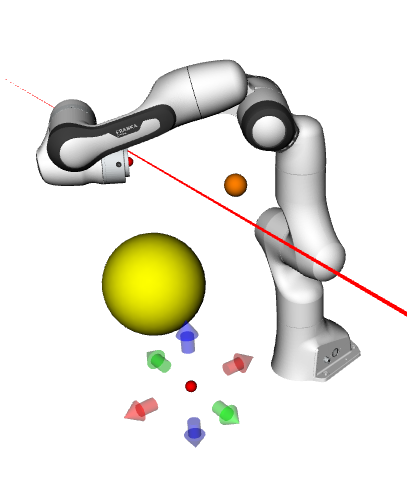
\includegraphics[width=0.45\columnwidth]{baseLine_Fail}
	\caption{Robot configuration when reactive WBQP controller (baseline approach) fails to find a solution.}
	\label{fig:robot fail}
\end{figure}

\section{Experimental Results}\label{sec-chap5:experiments}
Our goal is to highlight the main drawback of reactive WBQP discussed in the conclusions of \cref{chap:adaptive gains} and \cref{chap:robust qp}: the non-handling of potential conflict between constraints which may lead to infeasibility. In particular, the distance constraint formulated as ECBF assumes that $\confDDot\inR^n$, namely infinite deceleration capabilities, whereas $\confDDot$  often belongs to a subset  $U\subset\mathbb{R}^n$ constituted by the joint acceleration limits, torque bounds as well as other constraints. Conversely, the MPC allows solving this potential conflict by accounting for these constraints along the preview horizon and shaping the optimal targets $\command$ that fulfill those constraints.  %Unfortunately, the size of the command vector increases (and correspondingly the matrices $\Bd$ and $\stackBd$) which leads to high the MPC computation time. %as shown in~\eqref{eq:task&joint space QP with constraints} which results $\confDDot\in U\subset \mathbb{R}^n$ This situation is particularly appealing when $\confDDot\in U$ where $U$ is only a subset of $\mathbb{R}^n$. 

To validate our approach, we run simulations on the robotic arm Panda. The MPC \cref{eq:compact MPC} is implemented using COPRA library\footnote{\url{https://github.com/jrl-umi3218/copra}}. The current c++ implementation allows running the MPC in a separate thread. 
%The latter will then generate optimal targets $\eepositionOpt, \confOpt$. 
We have chosen to formulate the WBQP as in \cref{eq:task&joint space QP with constraints} to ensure dynamic consistency while tracking the MPC output. %Rather than considering the unconstrained QP~\cref{eq:task&joint space QP without constraints}, we have chosen to formulate the constrained QP~\cref{eq:task&joint space QP with constraints} in order to ensure dynamic consistency  while tracking $\eepositionOpt, \confOpt$ by the end-effector and posture tasks such that
More importantly, we consider the case where the end-effector has to avoid collision with a ball in its workspace. Let us denote $\bm{p}_{\rm ball}\inR^3$ the coordinates of the center of the ball and $r>0$ its radius. The distance between the end-effector and the ball surface is then 
\begin{equation}
	\delta(\conf) = \bm{n}_{\bm{\delta}}\tp\left(\eeposition - \bm{p}_{\rm ball}\right) - r \inR
\end{equation}
 with $\bm{n}_{\bm{\delta}}=\frac{\eeposition - \bm{p}_{\rm ball}}{||{\eeposition - \bm{p}_{\rm ball}}||}\inR^3$ is a unit vector. Consequently, to avoid the collision, the distance $h_{\rm coll}$ in \cref{eq:distance constraint forward kinematics} must fulfill
 \begin{equation}\label{eq:distance to collision constraint MPC}
 	h_{\rm coll}=\delta(\conf) - \delta_{\min} \geq0 
 \end{equation}
Then, $\dot{h}$ and $\ddot{h}$ are defined as in \cref{eq:distance constraint forward vel,eq:distance constraint forward acc} where $\mathbf{J}^{h_{\rm coll}}=\bm{n}_{\bm{\delta}}\tp\eeJac$ and $\mathbf{\dot{J}}^{h_{\rm coll}}=\bm{n}_{\bm{\delta}}\tp\eeJac + \bm{n}\tp\eeJacDot$. To make the problem more appealing, another constraint is defined for the robot CoM $\bm{CoM}(\conf)\inR^3$ to be upper bounded along the $X$-axis. This is achieved by keeping the distance $h_{\rm com}$ positive
\begin{equation}\label{eq:com constraint along X-MPC}
	h_{\rm com} = \bm{n}_{\rm com}\tp \bm{CoM}(\conf) + {CoM}_{X_{\max}} >0
\end{equation}
where $\bm{n}_{\rm com}\tp = \begin{bmatrix}
	-1 &0 &0
\end{bmatrix}\inR^3$ is a normal vector and ${CoM}_{X_{\max}}=0.2$~cm. The CoM constraint Jacobian $\mathbf{J}^{h_{\rm com}}=\bm{n}_{\rm com}\tp\mathbf{J}^{{\rm com}}\inR^{1\times n}$ and $\mathbf{\dot{J}}^{h_{\rm com}}=\bm{n}_{\rm com}\tp\mathbf{\dot{J}}^{{\rm com}}\inR^{1\times n}$ with $\mathbf{J}^{{\rm com}}\inR^{3\times n}$ the CoM Jacobian.
By constraining the CoM in \cref{eq:com constraint along X-MPC}, the robot is less free to stretch the arm to skirt the ball, and thereby it demands more complex motion for the robot to fulfill both constraints while taking into account the hardware limitations.   
 

The experiment scenario consists in generating random reference Cartesian targets $\REF{\eeposition}\inR^{m}$ ($\REF{\eevelocity}=\REF{\eeacceleration}=\zeros)$ that are forwarded to MPC\footnote{$\REF{\conf}\inR^{n}$ ($\REF{\confDot}=\REF{\confDDot}=\zeros$) is also forwarded to MPC and denotes a given reference posture with an elbow-up configuration.}. These random targets aim to lead the end-effector into a collision with the ball and the CoM to reach its maximum boundary (\cref{fig:pannda&yellowball&CoM}).
The meta-parameters of MPC and WBQP used in the experiment are shown in \cref{tab:MPC-QP parameters}.
\begin{figure}
	\centering
	\subfloat[]{
		\includegraphics[width=0.49\columnwidth]{hcoll_mpc2}
		\label{subfig:hcoll and hdotcoll MPC}}
	%	\hfil
	\subfloat[]{
		\includegraphics[width=0.49\columnwidth]{hcom_mpc2}
		\label{subfig:hcom and hdotcom MPC}}
	\caption{Time evolution of $h_{*}$ (blue) and $\dot{h}_{*}$ (orange) in the case of closed-loop MPC-WBQP control scheme:~\subref{subfig:hcoll and hdotcoll MPC} $h_{\rm coll}$ and $\dot{h}_{\rm coll}$,~\subref{subfig:hcom and hdotcom MPC} $h_{\rm com}$ and $\dot{h}_{\rm com}$. The colored bands correspond to the current assigned $\REF{\eeposition}$.}
	\label{fig:hcoll and hcom MPC}
\end{figure}
\begin{figure}
	\centering
	\subfloat[]{
		\includegraphics[width=0.49\columnwidth]{hcoll_prediction}
		\label{subfig:hcoll prediction MPC}}
	%	\hfil
	\subfloat[]{
		\includegraphics[width=0.49\columnwidth]{hcom_prediction}
		\label{subfig:hcom prediction MPC}}
	\caption{Time evolution of $h_{*}$ (blue solid) and the its predictions (colored dotted-solid) along different preview horizon in the case of closed-loop MPC-WBQP control scheme for $t\in\left[0.7,3\right]$~s (first colored band in \cref{fig:hcoll and hcom MPC}).~\subref{subfig:hcoll prediction MPC} $h_{\rm coll}$.~\subref{subfig:hcom prediction MPC} $h_{\rm com}$.}
	\label{fig:hcoll and hcom  prediction MPC}
\end{figure}
\begin{figure}
	\centering
	\subfloat[]{
		\includegraphics[width=0.33\columnwidth]{X_mpc2}
		\label{subfig:X}}
%	\hfil
	\subfloat[]{
		\includegraphics[width=0.33\columnwidth]{Y_mpc2}
		\label{subfig:Y}}
%	\hfil
	\subfloat[]{
		\includegraphics[width=0.33\columnwidth]{Z_mpc2}
		\label{subfig:Z}}
	\caption{Reference Cartesian target $\REF{\eeposition}$ (dashed blue), optimal Cartesian target $\eepositionOpt$ (orange) and end-effector position $\eeposition$ (blue).~\subref{subfig:X} X coordinate.~\subref{subfig:Y} Y coordinate.~\subref{subfig:Z} Z coordinate.}
	\label{fig:optimal target MPC}	
\end{figure}
\begin{figure}
	\centering
	\subfloat[]{
		\includegraphics[width=0.33\columnwidth]{endEff_X_prediction}
		\label{subfig:X prediction}}
	%	\hfil
	\subfloat[]{
		\includegraphics[width=0.33\columnwidth]{endEff_Y_prediction}
		\label{subfig:Y prediction}}
	%	\hfil
	\subfloat[]{
		\includegraphics[width=0.33\columnwidth]{endEff_Z_prediction}
		\label{subfig:Z prediction}}
	\caption{End-effector position $\eeposition$ (blue solid) and its predictions (colored dotted-solid) along different preview horizon in the case of closed-loop MPC-WBQP control scheme for $t\in\left[0.7,3\right]$~s (first colored band in \cref{fig:optimal target MPC}).~\subref{subfig:X} X coordinate.~\subref{subfig:Y} Y coordinate.~\subref{subfig:Z} Z coordinate.}
	\label{fig:endEff prediction MPC}	
\end{figure}
\subsection{Baseline Approach}
For comparison, we choose the baseline approach to be the reactive WBQP closed-loop control scheme shown in \cref{fig:MPC-QP}\subref{subfig:MPC-QP kinematic-controlled robot} without the MPC outer  loop.  WBQP is formulated as in~\cref{eq:task&joint space QP with constraints} to which we insert on-the-fly the collision and CoM constraints \cref{eq:collision constraint} and \cref{eq:com constraint along X-MPC} formulated as shown in \cref{eq:second order ODI distance}
\begin{align}
\label{eq:collision constraint formulated ODI}	\mathbf{J}^{h_{\rm coll}}\confDDot + \mathbf{\dot{J}}^{h_{\rm coll}}\confDot  +K_{\rm d}^{h_{\rm coll}}\dot{h}_{\rm coll} +K_{\rm s}^{h_{\rm coll}}h_{\rm coll} &\geq0, \ \text{if~} h_{\rm coll}\leq10~\text{cm},\\
\label{eq:com constraint formulated ODI}	\mathbf{J}^{h_{\rm com}}\confDDot + \mathbf{\dot{J}}^{h_{\rm com}}\confDot  +K_{\rm d}^{h_{\rm com}}\dot{h}_{\rm com} +K_{\rm s}^{h_{\rm com}}h_{\rm com} &\geq0, \ \text{if~} h_{\rm com}\leq3~\text{cm},
\end{align}
 where the constraints gains are computed as in \cref{eq:adaptive gain equation}. The results are shown in \cref{fig:hcoll and hcom time evolution-QP baseline}. \cref{fig:hcoll and hcom time evolution-QP baseline}\subref{subfig:hcoll} and \cref{fig:hcoll and hcom time evolution-QP baseline}\subref{subfig:hcom} show that when the collision and com constraints~\cref{eq:collision constraint formulated ODI} and \cref{eq:com constraint formulated ODI}, respectively, are inserted  with low initial velocities $\dot{h}_{\rm coll}$ and $\dot{h}_{\rm com}$ then the joint deceleration needed is feasible and WBQP finds a solution $\confDDot$ within the hardware limits. In this case, the collision and com constraints are compatible with the hardware limits. However, when the initial velocity is high ($\dot{h}_{\rm coll}=-1.2$~m/s shown with a thick circle), then the necessary joint deceleration to stop at the boundary is not compatible with the hardware limits, and thereby the WBQP fails to find a solution (\cref{fig:robot fail}).  


\begin{figure}
	\centering
	\includegraphics[width=0.6\columnwidth]{qRef_mpc}
	\caption{Reference posture target $\confOpt$ computed by MPC and tracked by the WBQP posture task \cref{eq:optimal posture target for QP}.}
	\label{fig:optimal posture target MPC}
\end{figure}
\begin{figure}
	\centering
	\includegraphics[width=0.32\columnwidth]{5_mpc2}
	\includegraphics[width=0.32\columnwidth]{7_mpc2}
	\includegraphics[width=0.32\columnwidth]{4_mpc2} \\
	\includegraphics[width=0.32\columnwidth]{2_mpc2}
	\includegraphics[width=0.32\columnwidth]{3_mpc2}
	\includegraphics[width=0.32\columnwidth]{6_mpc2} 
%	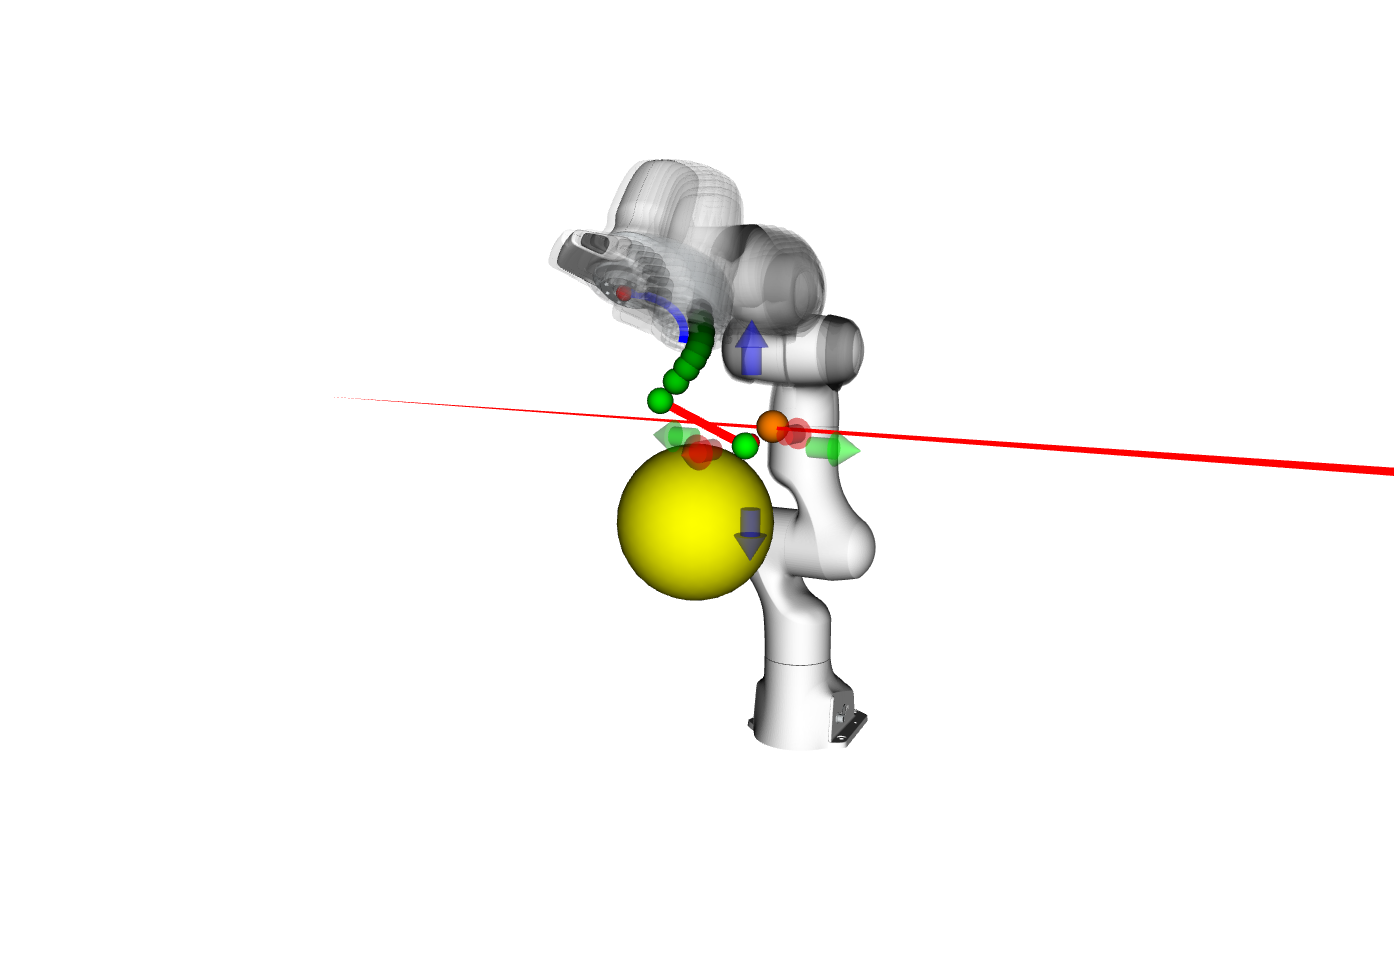
\includegraphics[width=0.25\columnwidth]{4.png}
%	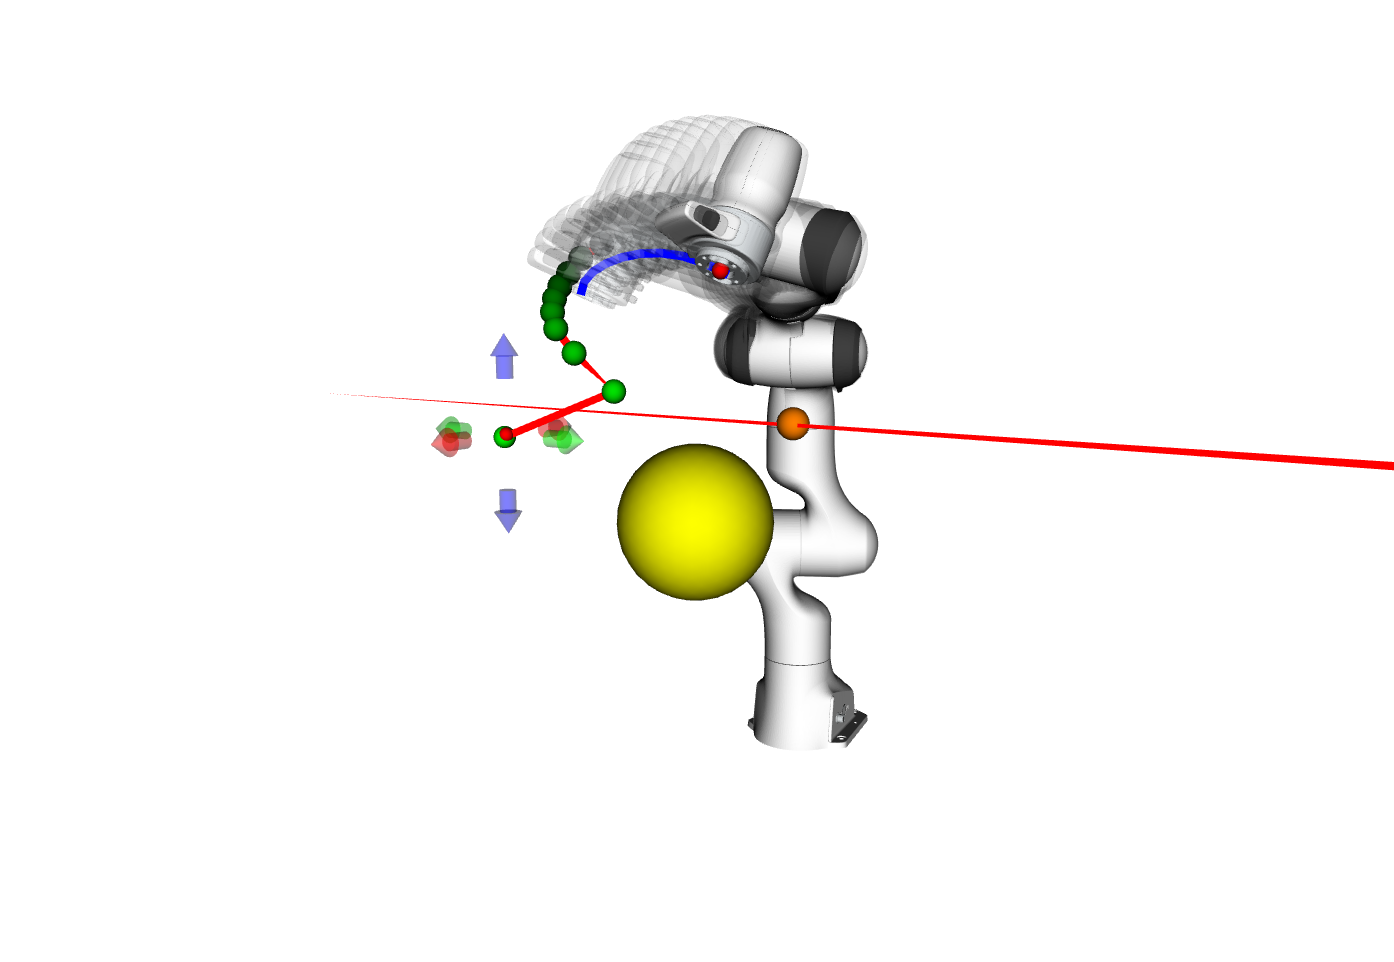
\includegraphics[width=0.2\columnwidth]{5.png}
\caption{Different screenshots of the closed-loop MPC-WBQP resulting motion. The shadowed Pandas are the robot states prediction along the preview horizon. The blue trajectory denotes the predicted end-effector $\eeposition$ position, and the predicted optimal Cartesian targets $\eepositionOpt$ are shown with graduated-green points.}
\label{fig:MPC-QP motion}
\end{figure}
\begin{figure}
	\centering
	\subfloat[]{
		\includegraphics[width=0.49\columnwidth]{hcoll_hcom_zoom_mpc2}
		\label{subfig:hcoll hcom zoomed}
	}
	\subfloat[]{
		\includegraphics[width=0.5\columnwidth]{slackness_mpc2}
		\label{subfig:slackness}
	}
	\caption{Zoom-in of $h_{*}$ near the boundary $h_{*}=0$ (dashed red) and the corresponding slackness.~\subref{subfig:hcoll hcom zoomed} $h_{\rm coll}$ (blue) and $h_{\rm com}$ (orange).~\subref{subfig:slackness} Slackness of the constraint \cref{eq:collision constraint MPC} (blue, left ordinate axis) and \cref{eq:com constraint MPC} (orange, right ordinate axis).}
	\label{fig:hcoll and hcom MPC zoomed + slackness}
\end{figure}
\begin{figure}
	\centering
	\includegraphics[width=0.6\columnwidth]{mpc_durationZ}
	\caption{MPC computation time (blue), the mean (red) and the standard deviation (dashed-yellow). The mean is $11.09$~ms with a standard-deviation of $1.22$~ms.}
	\label{fig:mpc duration}
\end{figure}
%\begin{figure}
%	\centering
%	\includegraphics[width=0.75\columnwidth]{slackness_mpc}
%	\caption{Slackness of the constraint \cref{eq:collision constraint MPC} (blue, left ordinate axis) and \cref{eq:com constraint MPC} (orange, right ordinate axis). }
%	\label{fig:slackness MPC}
%\end{figure}
\subsection{Closed-loop MPC-WBQP}
 For the MPC implementation, the state and command vectors are
\begin{equation}\label{eq:state and command for MPC-experiment}
	\state= \begin{bmatrix}
		\eeposition \\ \eevelocity \\ \conf \\ \confDot \\ h_{\rm coll} \\ \dot{h}_{\rm coll} \\ h_{\rm com} \\ \dot{h}_{\rm com} 
	\end{bmatrix}\inR^{2m+2n+4=24}, \ \command = \begin{bmatrix}
		\bm{\delta} \\ \eepositionOpt \\ \confOpt
	\end{bmatrix}\inR^{d+m+n = 19}.
\end{equation}

The matrices $\mathbf{A}_c$ and $\mathbf{B}_c$ of the dynamic model in \cref{eq:continuous-time DS} are adapted to $\state$ and $\command$ vectors in \cref{eq:state and command for MPC-experiment}. In particular, $\ddot{h}_{\rm coll}$ and $\ddot{h}_{\rm com}$ are computed as in \cref{eq:distance constraint forward acc}, and the constraints \cref{eq:distance to collision constraint MPC} and \cref{eq:com constraint along X-MPC} are formulated as in \cref{eq:MPC distance constraint}.
The collision and CoM constraint are formulated as shown in \cref{eq:MPC distance constraint}
\begin{align}
\label{eq:collision constraint MPC}	\dot{h}_{{\rm coll}_i} + \alpha h_{{\rm coll}_i}  &\geq 0 \\
\label{eq:com constraint MPC}	\dot{h}_{{\rm com}_i} + \alpha h_{{\rm com}_i}  &\geq 0
\end{align}
The slack variables relax joint position constraint \cref{eq:MPC joint-pos constraint}, joint velocity constraint \cref{eq:MPC joint-vel constraint}, and collision and CoM constraints \cref{eq:collision constraint MPC} and \cref{eq:com constraint MPC}, respectively, which makes the slack variables dimension $d=n+2=9$.

 WBQP is formulated as in \cref{eq:task&joint space QP with constraints} without considering the collision and CoM constraints formulated as ODI in \cref{eq:collision constraint formulated ODI} and \cref{eq:com constraint formulated ODI}, respectively. 
Note that we could add the collision constraint and CoM constraints formulated as second-order ODI as shown in \cref{chap:adaptive gains} to WBQP as a supplementary safety layer. However, we chose to ignore them in WBQP to explicitly show the effect of the MPC-based reference governor on constraints satisfaction. 
 
 The discretization time step is taken $\deltaT = 0.12$~s with $N=10$ steps ($T_{\rm preview}=1.2$~s).
\subsubsection{MPC Optimal Outputs Evolution}
The time evolution of $h_{\rm coll}$, $\dot{h}_{\rm coll}$, $h_{\rm com}$ and $\dot{h}_{\rm com}$ is shown in \cref{fig:hcoll and hcom MPC}. $h_{\rm coll}$ and $h_{\rm com}$ reach smoothly their boundaries with zeros velocity. Comparatively, to the baseline approach in \cref{fig:hcoll and hcom MPC}, $\dot{h}_{\rm coll}$ and $\dot{h}_{\rm com}$ are not allowed to grow excessively because the deceleration starts earlier. This effect is illustrated in   \cref{fig:hcoll and hcom  prediction MPC} which shows the current $h_{\rm coll}$ and $h_{\rm com}$ with their predictions along different preview horizon. $h_{\rm coll}$ and $h_{\rm com}$ predictions either converge smoothly  toward the boundary  or stop before it. 
More concretely, the MPC output optimal targets $\eepositionOpt$  and $\confOpt$ that account for the hardware limitations, the collision and CoM constraints, and enforces them along the preview horizon. \cref{fig:optimal target MPC} shows how the MPC  computes $\eepositionOpt$ a pathway tracked by WBQP end-effector task \cref{eq:optimal Cartesian target for QP} and which deviates from $\REF{\eeposition}$ if the constraints require that (see colored bands in \cref{fig:hcoll and hcom MPC} and \cref{fig:optimal target MPC}). An example of $\eeposition$ predictions is shown in \cref{fig:endEff prediction MPC}. Correspondingly to \cref{fig:hcoll and hcom  prediction MPC},  $\eeposition$ predictions tend be constant after $t=1.5$~s stop the end-effector motion as $h_{\rm coll}$ and $h_{\rm com}$ are close to the their boundary.
In addition, the optimal posture target $\confOpt$ in \cref{fig:optimal posture target MPC} is varying as well to fulfill the constraints. From this perspective, the WBQP posture task \cref{eq:optimal posture target for QP} is no longer a regularization task intended mainly to solve the remaining redundancies but also contributes (correspondingly to its weight $\weight_{\confDDot}$) to prevent collisions or hardware limits violation. Screenshots of the closed-loop MPC-WBQP resulting motion with the predicted states are shown in \cref{fig:MPC-QP motion}.

% The posture task is no longer a regularization task intended mainly to solve the remaining redundancies, it brings an interesting behavior for the reactive whole-body QP.

\subsubsection{Constraints Fulfillment}
Since the WBQP does not account for the collision and CoM constraints, it is important to analyze how well delegating constraints fulfillment to MPC is performing. This is even more crucial since \cref{eq:collision constraint MPC} and \cref{eq:collision constraint MPC} are handled as soft constraints. %\cref{fig:hcoll and hcom MPC zoomed} shows a zoom-in of $h_{\rm coll}$ and $h_{\rm com}$ time evolution near the boundary $h_{*}=0$. 
We can see from \cref{fig:hcoll and hcom MPC zoomed + slackness}\subref{subfig:hcoll hcom zoomed} that $h_{\rm coll}$ and $h_{\rm com}$ slightly overshoot the boundary $h_{*}=0$ ($\leq 5\cdot10^{-5}$~m) before converging back to the boundary thanks to the asymptotic convergence property ensured by the constraint formulation \cref{eq:com constraint MPC} and \cref{eq:collision constraint MPC}. This slight violation is due to three factors:  the slack variables, the non-modeled joint dynamics since the experiment is performed with a kinematic-controlled robot as already discussed in \cref{chap:robust qp}, and the low MPC running frequency comparatively to the WBQP (namely the constraint can be violated within one MPC computation iteration).
%Nevertheless, it seems to be highly due the second factor rather than the first one. 
\cref{fig:hcoll and hcom MPC zoomed + slackness}\subref{subfig:slackness} shows non-zero slackness of both constraints \cref{eq:collision constraint MPC} and \cref{eq:com constraint MPC}.  Interestingly, relaxing these constraints does not systematically imply their violation. In fact, $h_{\rm coll}$ is strictly positive for $t\in\left[27.5,40\right]$~s, yet the corresponding slack variable is continuously non-null. We argue that this is because all the constraints are permanently introduced in MPC QP. Hence, the kinematic constraints can be active even when they are far from their boundaries and be potentially relaxed.
%the slackness is in terms of velocity and not in terms of distance: relaxing the velocity is less critical in the long run than relaxing the distance. 
The slack variables relative to the $\confDot$ constraints are not plotted because they are null (i.e., joint-position and velocity bounds enforced as hard constraints).
\subsubsection{Computation Time and Prediction Accuracy} 
Let us now analyze the prediction accuracy of our MPC-WBQP control scheme. We recall that we assume that the Jacobians and EoM matrices and vectors remain constant along the preview horizon to have a linear model for the MPC. From \cref{fig:hcoll and hcom  prediction MPC} and \cref{fig:endEff prediction MPC}, we can see that each current state matches accurately the prediction during at least 3 epochs (i.e., during $3\times 120 = 360$~ms). Beyond that, the prediction accuracy decreases since the conservatism effect may be more predominant\footnote{The highest prediction error is observed in \cref{fig:endEff prediction MPC}\subref{subfig:Z prediction} which is only $5$~cm at the end of the preview horizon $T_{\rm preview}=1.20$~s.}. This accuracy is due to the relatively low MPC computation time shown in \cref{fig:mpc duration} which allows refreshing the MPC computation at an average frequency of $90.21$~Hz. The computation time depends mainly on the size of $\stackCommand$ which is related to the number of prediction steps $N$ and the size of the command vector $\command$. In particular, in our simulation, $\stackCommand\inR^{209}$. Hence, improving the computation time boils down to either reducing $\command$ vector size or decreasing the length of the preview horizon. The first option is tricky as $\command$ size depends mostly on the robot DoF number and tasks dimension to be controlled. Another possibility is to lower the dimension of the slack variables $d$  by rendering some constraints hard, which may endanger the MPC feasibility. On the other hand, the second option alters the prediction abilities and approaches the myopic WBQP. Balancing between the prediction capabilities, MPC feasibility, and the computation time is a well-known dilemma that generally depends on the robot, the application, and the case-study.    


%In task-space, the deceleration is due to the deviation of the optimal target $\eepositionOpt$ from $\REF{\eeposition}$ if the latter leads $h_{\rm coll}$ and/or $h_{\rm com}$ to reach their boundaries. Thanks the preview horizon, the MPC predicts the future states and enforces the hardware limitations, and the collision and CoM constraints along the preview horizon. As shown in \cref{fig:optimal target MPC},  % the collision constraint and/or the  the predicted $h_{\rm coll}$ and $h_{\rm com}$ are approaching the zero boundary. 
%This de Since the hardware limitations are enforced as hard constraints, the dece lead the robot into collision. computed by MPC that the consequence of translated into a deviat 

%TODO: the velocity $\dot{h}_{\rm coll}$ is not allowed to grow excessively which is interpreted as the deceleration is performed earlier



%Results points:
%\begin{itemize}
%%	\item $h_{\rm coll}$ and $h_{\rm com}$ time evolution with MPC-QP approach
%%	\item $\REF{\eeposition},\eepositionOpt, \eeposition$ time evolution
%%	\item Slack variables relative to  $h_{\rm coll}$ and $h_{\rm com}$ constraints
%%	\item Screenshots of the robot with MPC
%%	\item Plot of predictions 
%%	\item Modify the formulation of the constraint relative to q: CBF (asymptotic stability and forward invariance) + optimized slack variables=
%%	\item MPC and QP computation time w.r.t $N$ 
%\end{itemize}

%\begin{itemize}
%	\item Why QP-based MPC: to account explicitly for constraints 
%	\item Compare with~\cite{grandia2021icra}, more importantly\cite{zeng2021acc2}. General citation~\cite{kleff2021icra,minniti2022ral} also \cite{bemporad1998tac} for the argumentation
%	\item See feasibility explanation in~\cite{zeng2021acc1,zeng2021acc2} 
%%	\item How to initialize the initial state $\state_{0}$
%%	\item The current c++ implementation allows choosing whether or not to run the MPC in a separate thread!
%%	\item The MPC implementation is performed using the COPRA library
%%	\item The choice of $N$ and $\deltaT$.
%%	\item Targets maybe outside the robot workspace. 
%%	\item The motion dynamics is tuned using the MPC cost-function weights rather than Whole-body QP task gains.
%%	\item The resulting motion is complex: the robot does not move in a straight-line like motion. 
%%	\item The MPC runs in a separate thread at a low frequency such that it launches a new computation right after finishing the previous one. In simulation the MPC runs at approximately $40$~Hz. \textbf{When we reduce the slack variable dimension to $d=9$ instead of $d=16$ by reformulating the joint-position constraint formulation in terms of velocity, the MPC computation time drops from $25$~ms to $10$~ms which enables the MPC to run at approximately $100$~Hz.}
%%	\item MPC Feasibility is ensured by means of slack variables. Relaxing the constraints is mainly to ensure that MPC feasibility if $\state_{0}$ violates the constraints due to non-modeled dynamics, noise or communication delays.  Yet, this is still better than using QP with relaxed constraints since it only guarantees point-wise feasibility without any preview of the future states~\cite{zeng2021acc1}.
%\end{itemize}
\section{Conclusion}\label{sec-chap5:conclusion}
In this chapter, we proposed a solution for constraints incompatibility, a well-known issue of multi-objective QP-based control approaches. To handle the potential conflict between constraints, our method consists of implementing an MPC-based reference governor which encapsulates the inner loop constituted by the WBQP controller and the robot. Based on the closed-loop dynamics of the tasks and constraints,  MPC outputs tasks' optimal targets to be tracked by multi-objective WBQP such that the hardware limits and safety constraints are enforced forward in time along the preview horizon. In particular, we showed that the optimal end-effector Cartesian targets avoid collision with an obstacle and keep the robot CoM bounded without even considering these constraints in the WBQP controller.
The proposed closed-loop MPC-WBQP control scheme outperforms the purely reactive (myopic) WBQP, where the constraints introduced online may lead to an empty feasibility domain. 

Despite the conservativeness of our method to keep the MPC model linear, we showed that the state's prediction accuracy justifies the soundness of our assumptions. 
In this context, future works will be conducted to enhance the MPC with a Jacobians prediction scheme that will considerably lower the conservativeness and improve the prediction precision. Hierarchical architecture proposed in~\cite{li2021ral} can also be a good compromise between prediction accuracy and computation simplicity. Moreover, experiments on Panda robot shall be performed.
%lower this conservatism by considering prediction models for the Jacobians and EoM matrices which enables to have a more accurate prediction. 
Also, establishing/breaking/maintaining contacts while moving~\cite{romualdi2022icra} is an interesting continuation topic of the presented work. 

In addition, we so far considered only tasks whose errors evolve in a Euclidean space. Typically, the orientation task error evolves in a non-Euclidean manifold, preventing straightforwardly including them into the current MPC linear implementation. Research work is currently conducted in this direction based on predicting the orientation of the local tangent space to exploit its Euclidean properties. 
Furthermore, theoretical studies need to be performed to analyze the closed-loop MPC-WBQP stability with sufficient conditions on the existence of solutions.

The next chapter introduces a strategy to unify observation and control. This strategy is based on a new idea of \emph{tasks-interdependency} in the context of multi-objective QP control. Namely, we intend to formulate a task whose reference is the output of another task. This new concept of multi-objective QP control framework allows us to combine tasks that may be \emph{coupled}: \emph{estimation} and \emph{tracking}, for instance. We then show how this new idea is judiciously exploited to formulate human-robot handover control. 
%the MPC model is based on the closed-loop dynamics of the tasks and constraints of interests and which is obtained by the closed-form solution an unconstrained weight-prioritized QP. 
%Thanks to its preview horizon, the MPC acts then as a constraints manager by outputting task optimal targets which fulfill the constraints. 
%TODO: - the appraoch outperforms the purely reactive (myopic) QP where the constraints introduced online may lead to an empty constraint set and thereby to QP infeasiblity. The results shows promising results despite the rough approximation made to keep the MPC linear.
%TODO:- see Niels email for constraints managing.   
%$$
%\weight_1^2 \norm{\qjacobian \qaccelerations  - \left( \PD{\eeacceleration} - \qjacobianDot \CUR{\qvelocities} \right)} 
%$$
%whereas the second objective aims to track PD joint accelerations \eqref{eq::jointspacePD} with weight $\weight_2^2>0$
%$$
%\weight_2^2 \norm{\identityMatrix \qaccelerations - \PD{\qaccelerations}}$$




%Combining the two weighted objectives \eqref{eq::taskspacePD} and \eqref{eq::jointspacePD},
%the classical quadratic problem~(QP) representing the whole-body controller writes
%\begin{IEEEeqnarray}{rCl}
%	\label{eq::mainQP}
%	\CUR{\qaccelerations}
%	= & \argmin_{ \qaccelerations } \hspace{0.2cm} & %todo \frac{1}{2} 
%	\norm{
%		\begin{bmatrix}
%			\weight_1 \qjacobian \\
%			\weight_2 \, \identityMatrix
%		\end{bmatrix}
%		\qaccelerations -
%		\begin{bmatrix}
%			\weight_1 \left( \PD{\eeacceleration} - \qjacobianDot \CUR{\qvelocities} \right) \\
%			\weight_2 \PD{\qaccelerations} 
%		\end{bmatrix}
%	}
%	\hspace{0.4cm}
%	%\nonumber 
%	\\ %############################################
%	& \text{s.t.} & 
%	%& \text{s. t. } &  
%	\qaccelerationsLowerBound \leq \qaccelerations \leq \qaccelerationsUpperBound
%	\nonumber 
%	\\ %############################################
%	&  & 
%	\qtorquesLowerBound - \qcoriolisMatrix \CUR{\qvelocities} - \qgravityMatrix
%	\leq \qinertia \qaccelerations 
%	\leq \qtorquesUpperBound - \qcoriolisMatrix \CUR{\qvelocities} - \qgravityMatrix
%	\nonumber
%\end{IEEEeqnarray}
%which can also be written as
%\begin{IEEEeqnarray}{rCl}
%	\label{eq::mainQP}
%	\CUR{\qaccelerations}
%	= & \argmin_{ \qaccelerations } \hspace{0.2cm} & %todo \frac{1}{2} 
%	\norm{
%		\begin{bmatrix}
%			\weight_1 \identityMatrix, & 0 \\
%			0, & \weight_2 \identityMatrix
%		\end{bmatrix}
%		\left(
%		\begin{bmatrix}
%			\qjacobian \\
%			\identityMatrix
%		\end{bmatrix}
%		\qaccelerations -
%		\begin{bmatrix}
%			\PD{\eeacceleration} - \qjacobianDot \CUR{\qvelocities} \\
%			\PD{\qaccelerations} 
%		\end{bmatrix}
%		\right)
%	}
%	\hspace{0.4cm}
%	%\nonumber 
%	\\ %############################################
%	& \text{subject to } & 
%	%& \text{s. t. } &  
%	\qaccelerationsLowerBound \leq \qaccelerations \leq \qaccelerationsUpperBound
%	\nonumber 
%	\\ %############################################
%	&  & 
%	\qtorquesLowerBound - \qcoriolisMatrix \CUR{\qvelocities} - \qgravityMatrix
%	\leq \qinertia \qaccelerations 
%	\leq \qtorquesUpperBound - \qcoriolisMatrix \CUR{\qvelocities} - \qgravityMatrix
%	\nonumber
%\end{IEEEeqnarray}
%
\chapter{Human-Robot Handovers using Task-Space Quadratic Programming}\label{chap:handover qp}

%\begin{itemize}
%	\item Figure of task interdependency 
%\end{itemize}

In the previous chapter, we addressed the issue of constraints compatibility between the hardware limitations and kinematic constraints. Since this issue requires a look-ahead on the robot motion, our idea consisted of enhancing the reactive whole-body QP by an MPC-based reference governor. We showed how the latter modifies the tasks' references to ensure compatibility between constraints.

%In the previous chapter, we proposed a robust feedback closed-loop QP control formulation in the case of kinematic-controlled robots. Task and set robust stability have been formally proved and validated in real experiments. In the case of multi-objective control, robust stability of relaxed tasks has been also proved. 

Multi-objective control is the main beneficial property exploited from the robot's redundancy. This control paradigm enabled the robots to execute more than one task, thereby approaching the natural human abilities. More importantly,  it opened wide the field for robots to get involved in plenty of domains, which has increased their impact on the economy, education, health service quality, food delivery, ergonomy, tourism, etc. In particular, one of the currently very active trends in robotics is maximizing the interactions between humans and robots. Among the most challenging ones, seamlessly exchanging objects between a human and robot as \emph{giver} and \emph{receiver} agents through (bi-directional) handovers is of the most importance (\cref{fig:handover examples}). Indeed, handing objects between humans is a persistent daily interaction in almost all domains~\cite{ortenzi2021tro}. Therefore, embedding human-centered robotic systems in automation and services with handovers capabilities is a key enabler for rich cognitive interaction~\cite{ajoudani2018autonomousRobots,billard2019science}. Although human-human handover is an intuitive behavior, it is a result of complex and sophisticated learned social-cognitive communication channels~\cite{strabala2013jhrisc}. Grasping such complexity in an equivalent robot control formulation strategy is not a trivial problem.

In this chapter, we formulate the premises of a generic robot control-strategy that ensures high fidelity and reliability of reaching motion for bi-directional handover scenarios and guarantees adaptability w.r.t the handover location (HOL, i.e., the meeting point where the two handover agents exchange the object) as well as the object orientation. Particularly, our control formulation is handover-location knowledge free. We only assume that the object's structural properties and dimensions are known, and there exists a sensor that tracks the pose (Cartesian position and orientation) of the object in interest, e.g.~\cite{paolillo2018ral}. In \cref{sec-chap4:sota}, we go through the state-of-the-art of human-robot handover control formulations and their limitations which enables us to present our contribution in \cref{subsec-chap4:contribution} succinctly. Then, we present in \cref{sec-chap4:handover formulation} the details of our task-space QP-based handover controller. Finally, we implement our method on Panda robotic arm taking objects from a human operator in \cref{sec-chap4:experiments}. 
%\textbf{Keep this as a result}The proposed control formulation ensures a real-time adaptation of the robot to the human desired HOL and orientation. 
%Of course, our first constraints is to build on our existing task-space optimization (QP) formulation framework~\cite{bouyarmane2018tac,bouyarmane2019tro} that prove to be very powerful in an industrial context~\cite{kheddar2019ram} and a human-assistance context~\cite{bolotnikova2021sii}. 



%Remove some references...

\section{Human-Robot Handover: State-of-The-Art}\label{sec-chap4:sota}
How to \emph{codify} the human-robot handover process has been thoroughly addressed in the research community. The state of the art studies split the handover process in two main phases: the \emph{pre-grasping} phase~\cite{shibata1995roman,waldhart2015iros,mainprice2021roman,huber2008roman,shi2013rss,koene2014roman,remazeilles2015rss} and the \emph{grasping} phase~\cite{nagata1998icra,chan2013ijrr,medina2016humanoids,solak2019iros,costanzo2021frontiersRob-AI}.
%\begin{itemize}
%	\item  \emph{Pre-grasping phase}~\cite{shibata1995roman,waldhart2015iros,mainprice2021roman,huber2008roman,shi2013rss,koene2014roman,remazeilles2015rss}
%	\item \emph{Grasping phase}~\cite{nagata1998icra,chan2013ijrr,medina2016humanoids,solak2019iros,costanzo2021frontiersRob-AI}
%\end{itemize} 
Such a breakdown is chronological: the former focuses on estimating/predicting the human movement and planning the robot reaching motion toward the meeting point, whereas the latter consists of understanding the interaction forces (haptics) applied at the object by the two handing over agents during the exchange such that to ensure a stable grasping. In~\cite{medina2016humanoids} a \emph{retraction} phase is considered, which describes how the giver and receiver move away after the latter gets full control of the object. In this chapter, we are interested in the pre-grasping phase of the handover process. Yet, for an exhaustive handover survey, please refer to the excellent recent review in~\cite{ortenzi2021tro}.  

\begin{figure}
	\centering
	\includegraphics[width=0.65\columnwidth]{collage3}
	\caption{Different handover scenarios: handing food for patient (top-left~\cite{nemlekar2019icra}), sharing a tool for a mechanic (top-right~\cite{prada2014iros}), lending mustard (bottom-left~\cite{ortenzi2021tro}), giving a water bottle (bottom-right~\cite{medina2016humanoids}).}
	\label{fig:handover examples}
\end{figure}

The pre-grasping phase formulation involves two subsequent questions: (i) \emph{where} and \emph{when} the handover will take place; (ii) how to generate the reaching motion.  \emph{Where} to handover is denoted as the HOL (also known as the object transfer point~\cite{li2015rss,nemlekar2019icra}), whereas \emph{when} to handover depends on the agents synchronization to reach the handover location, and the elapsed time during the object release by the giver and the full object control by the receiver. Planning for the reaching phase (ii) depends highly on the HOL knowledge. 

Different approaches have been proposed to formulate the robot's reaching motion. Dynamic Movement Primitives (DMP) are among the most documented and well theoretically-grounded methods. They were introduced in~\cite{ijspeert2002icra,schaal2005springer} as a powerful tool to generate complex trajectories while converging to a goal-attractor. DMP have been recently exploited to learn from demonstration and generate human-like handover robotic movement~\cite{prada2014iros}, and to predict the HOL and time using an extended Kalman Filter~\cite{widmann2018ecc}. The drawback of DMP-based approaches is the high number of hyper-parameter to tune, especially in high dimensions. In addition, the use of DMP as a part of a closed-loop system has been barely studied where the majority of works consider it a planning block only forwarding the references for the controller~\cite{saveriano2021arxiv}.
Probabilistic Movement Primitives (Pro-MP), which is an extension of DMP to stochastic systems~\cite{paraschos2013anips}, have been used in~\cite{nemlekar2019icra} to estimate the HOL dynamically from the observed human motion. However, the resulting motion is not fluent, and the robot does not well anticipate the object. 

\cite{laplaza2021roman} used video recordings of robot-human handover to train an attention deep-learning model that predicts the human joint positions. However, no further details have been provided about how this prediction is used for the robot reaching-motion formulation. Based on vision object-recognition, using eye-in-hand vision,~\cite{rosenberger2021ral} proposed an object-independent approach that does not require the prior knowledge of the object dimension/shape. A gripper-mounted camera is used to detect and distinguish between the human agent's hand and the object leveraging a trained image-classifier. It also enables a safe grasping and gripper orientation. However, the approach is computationally demanding and suffers a high time response to detect the object, which is constrained to remain static. Eye-in-hand vision has also been adopted in~\cite{costanzo2021frontiersRob-AI} except that the approach is based on reactive visual servoing. The latter generates robot motion to minimize the error between the perceived object image and a priorly acquired image.
Interestingly, the HOL knowledge is not required for the control formulation. However, an image database of the exchanged objects must be collected priorly. In addition, the experiment showed that the robot motion is not sufficiently proactive because of the low image-sampling frequency, and the object must be inside the camera field-of-view. 

\cite{medina2016humanoids} trained a Dynamical System (DS) to predict the human motion based on real-time motion data observed during a time window. The HOL is estimated online to be the robot's closest point (among the predicted human trajectory). 
The handover controller is formulated as two coupled dynamical systems: the giver (master) converges to the estimated HOL, and the receiver converges to an attractor that depends on the master convergence error.
%Then, the closest point to the robot among the predicted trajectory is considered as the handover location. Two Dynamical systems for the human hand and robot end-effector motion modeling are learned from offline experiment data. Then, handover controller is formulated as a coupled dynamical systems: the giver (master) converges to the estimated handover location, and the receiver converges to an attractor that depends on the master convergence error. Two dynamical systems are also learned for the angular motion modeling for both human hand and robot end-effectors. Which is time consuming for collecting data.

%Discuss how the motion during the pre-grasping phase is generated: DMP, Planning, DS, etc. 


%Despite the huge amount of works addressing human-robot handover, one issue remains open: how to ensure/codify an adaptive behavior of the robot w.r.t to a human versatile intention on \emph{where} to exchange the object, aka \emph{HandOver Location} (HOL), with the robot, and in which configuration (\emph{orientation}).  
Many existing works required the knowledge of the HOL as a precondition for motion planning or control formulations of the pre-grasping phase. In particular, the HOL is often considered either as fixed (the robot moves systematically to a fixed spot to pick up the object) or pre-planned (real-time detection and estimation of the object's fixed location) (see Tables~1~\&~2 in~\cite{ortenzi2021tro}). There are works that provide HOL estimation and online prediction methods~\cite{prada2014iros,medina2016humanoids,vahrenkamp2016humanoids,maeda2017autonomousRobots,widmann2018ecc,nemlekar2019icra}. However, such existing approaches have at least one of the following shortcomings:
\begin{itemize}
	\item Collecting data sets to train motion prediction models;
	\item Time-consuming computations leading to a hashed or a slow handover motion; 
	\item Magic-numbers of hyper-parameters to tune;
	\item Conservatism in the handover-location prediction policy; 
	\item Non-systematic success of the handover performance (i.e., success rates);
	\item The object orientation at the HOL is often kept the same during the experiments;
	\item Knowledge of the HOL is required.
\end{itemize}
\subsection{Contribution}\label{subsec-chap4:contribution}
Our proposed approach is meant to mitigate the above issues. More concretely, it gathers the advantages from both methods in~\cite{costanzo2021frontiersRob-AI,medina2016humanoids}. Indeed, our handover formulation does not require the knowledge of the HOL. Conversely to~\cite{costanzo2021frontiersRob-AI}, our method ensures/codifies a real-time proactive and adaptive robot motion w.r.t the human versatile intention on \emph{where} to exchange the object with the robot and in which configuration (\emph{orientation}). In fact, our proposed idea relies on the concept of \emph{interdependent tasks} where the state of one task is forwarded as the reference for another task. More precisely, we formulate an \emph{observation task} that estimates either the human hand or object full-state (depending on who is the giver) in terms of pose, velocity and acceleration which are then forwarded as references for a \emph{trajectory-tracking task} for the robot end-effector to track. Leveraging multi-objective QP control paradigm, these two tasks run concurrently in a leader-follower fashion: the object (leader) moves and converges to the HOL while the robot end-effector (follower) moves proactively toward the object while adjusting its orientation accordingly. From this standpoint, our approach is similar to the coupled DS in~\cite{medina2016humanoids}. Conversely, our approach is computationally cheap and does not require the estimation of the HOL or separately learning human and robot DS models.
\section{Task-Space QP Handover Formulation}\label{sec-chap4:handover formulation}
In this section, we first explain our methodology. Then, we detail our handover control formulation.
\subsection{Handover Control Problem}
%In order to achieve object handover efficiently, the robot reaching-motion toward the HOL shall be synchronized with the object's motion to have a \emph{one-shot continuous and smooth motion}. If the HOL is known in advance, the control formulation resumes to perform simply a set-point task for the end-effector (eventually with a secondary pre-planned trajectory tracking task). Nevertheless, the HOL as well as the object orientation are highly versatile: they may change during the handover motion or between two successive processes depending on the human intention and her/his posture. Handing over an object can even be aborted by a human decision while moving. Hence, planning the robot motion is likely to fail in such conditions. Alternatively, a reactive control method is more suitable for its ability to adjust the robot motion in real-time. We denote by \emph{end-effector} the robot terminal link used to pick-up the object. It encompasses two-finger grippers, multi-finger hand and even a non-human like devices as a suction-cup or an electromagnetic gripper~\cite{pan2018haptics}.  	
%For this purpose, the HOL needs to be predicted or anticipated by the robot based on the object motion held by human. Moreover, handling the object pose constraints in terms of orientation is mandatory for the robot to orient its gripper accordingly. 

%These aspects are highly versatile: they may change during the handover motion or between two successive process depending on \emph{where, when and how} the human intends to perform the handover process. The latter can even be aborted while moving based on the human decision. Hence, planning the robot motion is doomed to fail in such conditions. Alternatively, a reactive control method are more suitable as it enables reactively to modify the robot motion in real-time.

Our approach is to tackle the human-robot handover problem from a reactive closed-loop control perspective. We denote by \emph{end-effector} the robot terminal link used to pick up the object. It encompasses two-finger grippers, multi-finger hands, and even non-human-like devices such as a suction cup or an electromagnetic gripper~\cite{pan2018haptics}.  	First, we explain the approach when the human is the giver. Then we show how the approach fits when s/he is the receiver. The HOL can be seen as an attractor toward which the object converges (steered by the human). Since the HOL is not known a priori, the robot end-effector can track the object's trajectory leading to a proactive motion such that when the object converges to the HOL, its trajectory becomes a point to which the end-effector converges. The same reasoning can be applied to orientation. The remaining question is how to obtain the object trajectory in terms of pose $\boldsymbol{\xi}_{\rm obj}\in\mathbb{R}^7$, linear and angular velocity $\boldsymbol{\alpha}_{\boldsymbol{\xi}_{\rm obj}}\in\mathbb{R}^6$ and linear and angular acceleration $\boldsymbol{\dot{\alpha}}_{\boldsymbol{\xi}_{\rm obj}}\in\mathbb{R}^6$? These terms are encompassed as the \emph{object full-state} 
\begin{equation}\label{eq:object full-state}
	\bm{s}_{\rm obj}=\begin{bmatrix}
		\boldsymbol{\xi}_{\rm obj}\\ \boldsymbol{\alpha}_{\boldsymbol{\xi}_{\rm obj}} \\ \boldsymbol{\dot{\alpha}}_{\boldsymbol{\xi}_{\rm obj}}
	\end{bmatrix}\in\mathbb{R}^{19}.
\end{equation} 
Often, $\bm{s}_{\rm obj}$ cannot be directly obtained by the sensors as they generally provide only $\boldsymbol{\xi}_{\rm obj}$. Hence, an estimation of $\bm{s}_{\rm obj}$ needs to be constructed from $\boldsymbol{\xi}_{\rm obj}$, and it is denoted as %$\bm{s}_{\rm obs}$
\begin{equation}\label{eq:observer full-state}
	\bm{s}_{\rm obs}=\begin{bmatrix}
		\boldsymbol{\xi}_{\rm obs}\\ \boldsymbol{\alpha}_{\boldsymbol{\xi}_{\rm obs}} \\ \boldsymbol{\dot{\alpha}}_{\boldsymbol{\xi}_{\rm obs}}
	\end{bmatrix}\in\mathbb{R}^{19}.
\end{equation}
To this end, the observation task is formulated as a PD controller that drives 
$\boldsymbol{\xi}_{\rm obs}$ toward $\boldsymbol{\xi}_{\rm obj}$, e.g.,~\cite{paolillo2018ral}. While converging, the observation task outputs also $\boldsymbol{\alpha}_{\boldsymbol{\xi}_{\rm obs}}$ and $\boldsymbol{\dot{\alpha}}_{\boldsymbol{\xi}_{\rm obs}}$, e.g.,~\cite{pham2018pami}. $\bm{s}_{\rm obs}$ terms are then used as references for the trajectory-tracking task formulated for the end-effector. Note that the observation task allows generating trajectories for the orientation tracking without the need for offline planning methods~\cite{sciavicco2000book}. The same approach can be adapted if the human is a receiver. In such a case, the end-effector already holds the object, and its full-state is known by forward kinematics. Instead, the observation task constructs the full-state of the human hand~\cite{pham2018pami}. 

%Multi-objective task-space QP control has been extensively used as it enables to specify various tasks objectives while explicitly accounting for a set of convex constraints~\cite{bolotnikova2020roman}. 
In~\cite{bouyarmane2019tro}, one single QP controller can be formulated for multi-robot systems either decoupled or interacting using contact forces. In particular, the pre-grasping handover phase can be suitably formulated using the multi-robots QP by considering the robotic arm and the object as two decoupled robots. The former is a redundant multi-body system with all the joints actuated, and the latter is a floating-base rigid-body system. Moreover, the observation task is formulated for the object, and the trajectory-tracking task is formulated for the end-effector. 

The following subsections explicit in detail our approach. Here, we adopt the QP formulation in \cref{chap:adaptive gains} as the proposed formulation is not specific to the case of kinematic-controlled robots.
\subsection{Background}
Consider a redundant (fixed-base or floating-base) robot whose configuration $\genActConf$ is defined as in \cref{eq-chap0:gen act conf formal form}, and whose equation of motion is defined in~\cref{eq-chap0:equation of motion}.
%\begin{equation}\label{eq:equation of motion}
%	M(q)\ddot{q} + N(q,\dot{q}) = \tau + {\actJacContact}\tp f 
%\end{equation}
%where $M(q)\in\mathbb{R}^{n\times n}$ is the inertia matrix, $N(q,\dot{q})\in\mathbb{R}^{n}$ encompasses Coriolis, centrifugal and gravity torques, $\tau\in\mathbb{R}^{n}$ is the joint-torque, $\actJac_{\rm c}\in\mathbb{R}^{6\times n}$ is the Jacobian at the contact point and $f\in\mathbb{R}^6$ is the contact wrench. 
Let us consider the frame $\setR_{\rm ee}$ rigidly attached to robot end-effector and whose pose is   
\begin{equation}\label{eq:end-effector pose}
	\endEffPose=\begin{bmatrix}
		\endEffPosition \\ \endEffOrient
	\end{bmatrix}\in \mathbb{R}^7,
\end{equation}
where $\endEffPosition\inR^{3}$ is the end-effector Cartesian position and $\endEffOrient\inR^4$ is the unit quaternion representing the end-effector orientation.
The end-effector velocity and acceleration are given as 
\begin{align}\label{eq:end-effector vel and acc}
	\endEffPoseDot&=\begin{bmatrix}
		\endEffPositionDot \\ \endEffOrientDot
	\end{bmatrix} = \jacEndEff\genActConfDot\in \mathbb{R}^6, \\
	\endEffPoseDDot&=\begin{bmatrix}
		\endEffPositionDDot \\ \endEffOrientDDot
	\end{bmatrix} = \jacEndEff\genActConfDDot + \jacEndEffDot\genActConfDot\in \mathbb{R}^6,
\end{align}
where $ \jacEndEff = \begin{bmatrix}
	\jacLinEndEff \\\jacRotEndEff
\end{bmatrix}\inR^{6\times(6+n)}$ is the end-effector Jacobian where the superscripts $\textrm{ee-lin}$ and $\textrm{ee-rot}$ denote the linear and rotation parts of the Jacobian.
%	\begin{equation}\label{eq:end-effector transformation matrix}
	%		T_{\rm ee}(q)=\begin{bmatrix}
		%			R_{\rm ee}(q) & P_{\rm ee}(q) \\ 0 & 1 
		%		\end{bmatrix}\in SE(3)
	%	\end{equation}
%	where $P_{\rm ee}(q)\in \mathbb{R}^3$ and $R_{\rm ee}(q)\in SO(3)$ are the the end-effector Cartesian  coordinates and rotation matrix obtained by forward kinematics. 
%	Hereafter, the dependency on $\actConf$ is dropped. %Let us a define a surface $S$ to which the planar grippers motion belongs. Let us denote $n_S\in\mathbb{R}^3$ the normal vector to $S$ such that $n_S$ in $\setR_E$ are known (\cref{fig:gripper}).

Let us consider the object as a one-rigid-link robot with 6-DoF to which a frame $\frameObj$ is rigidly attached and whose pose is 
\begin{equation}\label{eq:object pose}
	\objPose=\begin{bmatrix}
		\objPosition \\ \objOrient
	\end{bmatrix}\in \mathbb{R}^7,
\end{equation}
%	\begin{equation}\label{eq:object transformation}
	%		T_{\rm obj}=\begin{bmatrix}
		%			R_{\rm obj} & P_{\rm obj} \\ 0 & 1 
		%		\end{bmatrix}\in SE(3)
	%	\end{equation}
where $\objPose$ is assumed to be provided by a sensor. 
Its velocity and acceleration are given as 
\begin{align}\label{eq:obj vel and acc}
	\objPoseDot&=\begin{bmatrix}
		\objPositionDot \\ \objOrientDot
	\end{bmatrix}\in \mathbb{R}^6, \
	\objPoseDDot=\begin{bmatrix}
		\objPositionDDot \\ \objOrientDDot
	\end{bmatrix}\in \mathbb{R}^6.
\end{align}
The object structural and dimension properties are known.

\subsection{Observation Task}\label{subsec-chap4:observation task}
%	{\color{red}The observation task error is zero when the object is static, otherwise it is bounded in an invariant set which size depends on the observation task gains.} 

%	Let us assume that the object is a free-floating base robot with 6 DoF to which a frame  $\setR_{\rm obj}$ is rigidly attached. Next, we assume that we have a sensor that measures the object pose $T_{\rm obj}$ in~\eqref{eq:object transformation}.
Let us consider an observed object to which a frame $\setR_{\rm obs}$ is rigidly attached whose pose is 
\begin{equation}
	\obsPose = 
	\begin{bmatrix}
		\obsPosition \\ \obsOrient
	\end{bmatrix}\in \mathbb{R}^7.  
\end{equation}
%	  Let us denote $\boldsymbol{\xi}_{\rm obj},\boldsymbol{\xi}_{\rm obs}\in\mathbb{R}^7$ the pose  in vector form of the observed and estimated object, respectively, such that 
%	\begin{equation}
	%		\boldsymbol{\xi}_{\rm obs} = 
	%		\begin{bmatrix}
		%			P_{\rm obs} \\ \quaternion_{\rm obs}
		%		\end{bmatrix}, \  
	%		\boldsymbol{\xi}_{\rm obj} = 
	%		\begin{bmatrix}
		%			P_{\rm obj} \\ \quaternion_{\rm obj}
		%		\end{bmatrix} 
	%	\end{equation}
%	where $P_{*}\in\mathbb{R}^3$ denotes the Cartesian coordinates of the corresponding frame origin.
% and $\quaternion_{\star} = \begin{bmatrix}
	%	\bar{\quaternion}_{\star} & \hat{\quaternion}_{\star} 
	%\end{bmatrix}^T\in\mathbb{R}^4$ is the quaternion parametrization of the corresponding frame orientation (w.r.t the world-frame) with $\bar{\quaternion}_{\star}\in\mathbb{R}$ and $\hat{\quaternion}_{\star}\in\mathbb{R}^3$ are the scalar and vector parts of $\quaternion_{\star}$. 	
	Assuming that the object velocity and acceleration in \cref{eq:obj vel and acc} are not provided by the sensor (which is likely the case), the observation task aims at constructing these non-measured states by estimating $\bm{s}_{\rm obs}$ in~\cref{eq:observer full-state}. 
	%	\begin{align}\label{eq:observed full-state}
		%		\bm{s}_{\rm obs} = \begin{bmatrix}
			%			\boldsymbol{\xi}_{\rm obs} \\ \alpha_{\boldsymbol{\xi}_{\rm obs}} \\ \dot{\alpha}_{\boldsymbol{\xi}_{\rm obs}}
			%		\end{bmatrix}
		%	\end{align}
	%	where 
	%	\begin{align}
		%		\alpha_{\boldsymbol{\xi}_{\rm obs}} = \begin{bmatrix}
			%			\dot{P}_{\rm obs} \\ \omega_{\rm obs}
			%		\end{bmatrix}\in\mathbb{R}^6, \  \dot{\alpha}_{\boldsymbol{\xi}_{\rm obs}} = \begin{bmatrix}
			%			\ddot{P}_{\rm obs} \\ \dot{\omega}_{\rm obs}
			%		\end{bmatrix}\in\mathbb{R}^6
		%	\end{align} 
	%with $\dot{P}_{\rm obs}, \ddot{P}_{\rm obs}$ denote the linear velocity and acceleration, and $\omega_{\rm obs}, \dot{\omega}_{\rm obs}$ denote the angular velocity and acceleration.  
	This is achieved by the observation task that steers $\obsPose$ toward $\objPose$ by keeping the observation error $\bm{e}_{\rm obs}$ as small as possible such that\footnote{$\obsOrient \ominus \objOrient^{-1}$ denotes the vector part of the quaternion product $\obsOrient\otimes\objOrient^{-1}$. Please, refer to \cref{sec-app:quaternion product} for more details.}
	\begin{align}\label{eq:observation error}
		\observTaskErr &= 
		\begin{bmatrix}
			\obsPosition-\objPosition \\ \obsOrient \ominus \objOrient^{-1}
		\end{bmatrix}\in \mathbb{R}^{6}.
	\end{align}
	Hence, the observation error velocity and acceleration are  given as
	\begin{align} 
	\observTaskErrDot = \obsPoseDot\inR^{6}, \ 
		\observTaskErrDDot = \obsPoseDDot\inR^{6}.
	\end{align}
	Let us define the observation task state  as 
	\begin{equation}
		\observTaskState = 	\begin{bmatrix}
			\observTaskErr \\	\observTaskErrDot
		\end{bmatrix}  \in \mathbb{R}^{12}
	\end{equation}
	Thus, the observation task is formulated as follows
	\begin{align}\label{eq:observation task dynamics}
		\observTaskStateDot &= 
		\begin{bmatrix}
			\zeros & \eye \\ \zeros & \zeros
		\end{bmatrix}\observTaskState + 
		\begin{bmatrix}
			\zeros \\ \eye
		\end{bmatrix} \observTaskErrFeedback, \\
		\label{eq:mu observartion task}\observTaskErrFeedback &=\observTaskErrDDot.
	\end{align}
 $\observTaskErrFeedback$ in~\eqref{eq:mu observartion task} is chosen to be a linear state feedback 
	\begin{equation}\label{eq:observation-task feedback law}
		\observTaskErrFeedback = - \begin{bmatrix}
			\mathbf{K}_{\rm s}^{\rm obs} & \mathbf{K}_{\rm d}^{\rm obs} 
		\end{bmatrix}\observTaskState = -\mathbf{K}^{\rm obs}\observTaskState,
	\end{equation}
	with $\mathbf{K}_{\rm s}^{\rm obs}, \mathbf{K}_{\rm d}^{\rm obs} \in \mathbb{R}^{6\times6}$ are diagonal positive-definite matrices denoting the stiffness and damping gains for the observation task. Replacing \cref{eq:observation-task feedback law} into \cref{eq:observation task dynamics} it yields to the following observation-task closed-loop dynamics
	\begin{align}
		\label{eq:observation-task closed-loop}\observTaskStateDot &= \mathbf{A}_{\rm obs}\observTaskState, \ \mathbf{A}_{\rm obs} = 
		\begin{bmatrix}
			\zeros & \eye \\ -\mathbf{K}_{\rm s}^{\rm obs} & -\mathbf{K}_{\rm d}^{\rm obs}
		\end{bmatrix}
	\end{align}
	with $\mathbf{A}_{\rm obs}$ Hurwitz~\cite{khalil2002NonLinearSystems}. Note that $\observTaskState$ only converges asymptotically to zero if the object is static ($\objPose$ constant). However, choosing high gain values typically enables a fast convergence and keeps $\norm{\observTaskErr}$ sufficiently small. 
	
	The benefits of the observation task are three folds: (i) allowing a bounded estimation of $\bm{s}_{\rm obs}$ in \cref{eq:observer full-state} given \cref{eq:mu observartion task,eq:observation-task feedback law,eq:observation-task closed-loop}; (ii) $\objPose$ is low-pass filtered by the closed-loop observation task dynamics~\eqref{eq:observation-task closed-loop}; (iii)  online generation of a smooth twice-differentiable trajectory\footnote{This is also known as a \emph{reference model}-based approach for trajectory references generation~\cite[Chapter 13]{khalil2002NonLinearSystems}. In addition, the trajectory feedforward terms are generated in real-time since the observation task is updated at the same frequency of QP ($1$~kHz) no matter the sampling frequency of the sensor.} for the Cartesian and orientation coordinates of $\setR_{\rm obs}$ frame without the needs of offline planning methods~\cite{sciavicco2000book}. The latter advantage is the \emph{core} idea presented in this paper: the observation task outputs trajectory references required by the trajectory-tracking task to achieve a proactive handover process. 
	
	Once having $\bm{s}_{\rm obs}$, we can compute the full-state for any other frame $\setR_{\star}$ attached to the object (for which the local pose $\boldsymbol{\xi}_{\star}^{\rm obs}$ is known) by simply applying the classical kinematic relations for position, velocity and acceleration\footnote{Note that the rigid body assumption implies that $\bm{\dot{p}}_{\star}^{\rm obs}=0$, $\mathbf{\dot{R}}_{\star}^{\rm obs}=0$, $\boldsymbol{\omega}_{\star} = \obsOrientDot$ and $\boldsymbol{\dot{\omega}}_{\star} = \obsOrientDDot$.}
	\begin{align}
		\label{eq:forward position}	\bm{p}_{\star} &= \obsPosition + \rotMatObs \bm{p}_{\star}^{\rm obs} \\
		\label{eq:forward velocity}	\dot{\bm{p}}_{\star} & = \obsPositionDot + \skewMat{\obsOrientDot} \rotMatObs \bm{p}_{\star}^{\rm obs} \\	
		\label{eq:forward acceleration}	\ddot{\bm{p}}_{\star} & = \obsPositionDDot +\skewMat{\obsOrientDDot} \rotMatObs \bm{p}_{\star}^{\rm obs}  + \skewMat{\obsOrientDot} \skewMat{\obsOrientDot}\rotMatObs \bm{p}_{\star}^{\rm obs}\\
		\label{eq:rotation matrix for grasp frame}\mathbf{R}_{\star} &= \rotMatObs\mathbf{R}_{\star}^{\rm obs}\\%\Rightarrow \dot{R}_{\star} = \skewMat{\omega_{\rm obs}}R_{\star}% \\
		\label{eq:rotation matrix derivatuve for grasp frame}\mathbf{\dot{R}}_{\star} &= \skewMat{\obsOrientDot}\mathbf{R}_{\star}
	\end{align}
	The transformations above allow computing the full-state of any frame used as a reference for the subsequent tasks described in the next subsections. 
	\subsection{Trajectory-Tracking Task}\label{subsec-chap4:trajectory tracking}
	The trajectory-tracking task describes how the end-effector frame $\frameEndEff$ tracks the position and orientation of the grasping frame $\setR_{\rm grasp}$
	%Let $\setR_{\rm grasp}$ be the grasping frame 
	rigidly attached to the object and whose pose is defined as 
	\begin{equation}
		\graspPose = \begin{bmatrix}
			\graspPosition \\ \graspOrient
		\end{bmatrix}\in\mathbb{R}^7.
	\end{equation}
	 $\graspPosition\in\mathbb{R}^3$ denotes the coordinates of the point where the end-effector grasps the object and  is computed from \cref{eq:forward position}, and $\graspOrient\inR^4$ is obtained from $\rotMatGrasp$ in \cref{eq:rotation matrix for grasp frame}. $\setR_{\rm grasp}$ velocity and acceleration are computed as 
	\begin{align}\label{eq:grasp vel and acc}
		\graspPoseDot&=\begin{bmatrix}
			\graspPositionDot \\ \graspOrientDot
		\end{bmatrix}\in \mathbb{R}^6, \
		\graspPoseDDot=\begin{bmatrix}
			\graspPositionDDot \\ \graspOrientDDot
		\end{bmatrix}\in \mathbb{R}^6
	\end{align}
	%	In order to efficiently perform the handover process, the robot should anticipate $P_{\rm grasp}$ location. This proactive behavior can be obtained by formulating a grasping-point-tracking task for the robot end-effector position $P_{\rm ee}$  where the trajectory references $P_{\rm grasp}$, $\dot{P}_{\rm grasp}$, $\ddot{P}_{\rm grasp}$ are computed according to~\eqref{eq:forward position}--\eqref{eq:forward acceleration} following from the observation task (\cref{subsec:observation task}).
	Let us define the trajectory-tracking task error as 
	\begin{align}\label{eq:grajectory tracking error}
		\trajTrackTaskErr &= 
		\begin{bmatrix}
			\endEffPosition -\graspPosition \\ \endEffOrient \ominus \graspOrient^{-1}
		\end{bmatrix}\in \mathbb{R}^{6},
	\end{align}
	and whose derivative is given as 
	\begin{align}\label{eq:grajectory tracking errorDot}
		\trajTrackTaskErrDot &= 
		\begin{bmatrix}
			\endEffPositionDot -\graspPositionDot \\ \endEffOrientDot - \graspOrientDot
		\end{bmatrix}= \endEffPoseDot-\graspPoseDot\in \mathbb{R}^{6}.
	\end{align}
	Let us denote the trajectory-tracking task state 
	\begin{align}\label{eq:grasping-point-tracking task state}
		\trajTrackTaskState = 
		\begin{bmatrix}
			\trajTrackTaskErr \\ 	\trajTrackTaskErrDot
		\end{bmatrix}\in\mathbb{R}^{12} 
	\end{align}
	Hence, the trajectory-tracking task dynamics is formulated 
	\begin{align}
		\trajTrackTaskStateDot &= 
		\begin{bmatrix}
			\bm{0} & \mathbf{I} \\ \bm{0} &\bm{0} 
		\end{bmatrix}\trajTrackTaskState+ 
		\begin{bmatrix}
			\bm{0} \\  \mathbf{I}
		\end{bmatrix} \trajTrackTaskErrFeedback \\
		\label{eq:mu grasping-point-tracking task}\trajTrackTaskErrFeedback  &=\endEffPoseDDot-\graspPoseDDot = \jacEndEff\genActConfDDot + \jacEndEffDot\genActConfDot - \graspPoseDDot
	\end{align}
	Then, choosing $\trajTrackTaskErrFeedback$ in \cref{eq:mu grasping-point-tracking task} as 
	\begin{equation}\label{eq:grasping-point-tracking task feedback law}
		\trajTrackTaskErrFeedback = - \begin{bmatrix}
			\mathbf{K}_{\rm s}^{\rm tt} & \mathbf{K}_{\rm d}^{\rm tt} 
		\end{bmatrix} \trajTrackTaskState = -\mathbf{K}_{\rm tt}\trajTrackTaskState,
	\end{equation}
	with $\mathbf{K}_{\rm s}^{\rm tt} , \mathbf{K}_{\rm d}^{\rm tt} \in\mathbb{R}^{6\times6}$ are diagonal positive-definite matrices denoting the stiffness and damping gains; it yields to the following trajectory-tracking task closed-loop dynamic
	\begin{equation}
		\label{eq:grasping-point-tracking-task closed-loop}\trajTrackTaskStateDot
		= \mathbf{A}_{\rm tt}\trajTrackTaskState, \ \mathbf{A}_{\rm tt} = 
		\begin{bmatrix}
			\mathbf{0} & \mathbf{I} \\ -\mathbf{K}_{\rm s}^{\rm tt} & -\mathbf{K}_{\rm d}^{\rm tt}
		\end{bmatrix},
	\end{equation}
	where $\mathbf{A}_{\rm tt}$ is Hurwitz. This enables a global asymptotic convergence of  $\trajTrackTaskState$ to the origin~\cite{khalil2002NonLinearSystems}. 
	
	In common trajectory tracking control, the trajectory is planned such that the initial reference trajectory pose is as close as possible to the current end-effector pose $\endEffPose(t_0)$ which indeed ensures that the tracking error $\trajTrackTaskErr(t_0)$ is small and thereby enforces the end-effector pose to stick on trajectory forward in time. However, when the trajectory starts far from the initial end-effector pose, the latter converges to the trajectory without lagging with exponential decay of the tracking error $\trajTrackTaskState$. This property enables the anticipatory motion of the end-effector, which moves proactively toward the object grasping position (see \cref{fig:robot and object}).
	\begin{figure}
		\centering
		\includegraphics[width=0.6\columnwidth]{explanation-scheme-legends-woAxis}
		\caption{Illustrative scheme showing the different frames $\frameWorld$, $\frameEndEff$, $\frameObj$, $\frameObs$ and $\frameGrasp$. The observed object is tracking the actual object, giving the sensor data. The end-effector tracks the observation task outputs yielding an anticipatory motion toward the HOL where it ultimately meets the object. The colored unit vectors in $\frameEndEff$ track their corresponding in $\frameGrasp$. The frames $\frameObj$ and $\frameObs$ are not in the same placement only for clear visualization purposes.}
		\label{fig:robot and object}
	\end{figure}

In this subsection, we assumed that the grasping point $\graspPosition$ coordinates are explicitly specified. However, we could have the case where $\graspPosition$ belongs to a line segment $\segLineGrasp\supset\setPgrasp$ where $\setPgrasp$ is a set of valid grasping points on the object contact surface along the symmetry axis directed by $\bm{u}_{\rm grasp}$ (\cref{fig:object without planes}). This is typically the case if we want the end-effector to grasp the object anywhere except where the human is holding. In this perspective, the task is considered to be achieved once the end-effector converges to $\setPgrasp$. This scenario can be broken down into two control objectives:  \emph{line-segment-tracking task} and \emph{grasping-set constraint}. The former consists of formulating a task to drive  $\endEffPosition$ toward $\segLineGrasp$ and the latter is meant to steer/maintain  $\endEffPosition$ inside $\setPgrasp\subset\segLineGrasp$.
\begin{figure}
	\centering
	\includegraphics[width=0.7\columnwidth]{object_woPlanes-woBackGronud}
	\caption{Object with the line segment $\segLineGrasp$ (dash-dotted orange) along which a set $\setPgrasp$ of the valid grasping region (highlighted with a yellow rectangle). $\normPlanU$ is denoted in yellow, and the red spheres denote the spots where the human is holding the object.}
	\label{fig:object without planes}
\end{figure} 
	\subsection{Grasping-Set-Tracking Task}\label{subsec-chap4:grasping-set-tracking}
	Hereafter, we only modify the translation part of the trajectory-tracking task formulation described in \cref{subsec-chap4:trajectory tracking}. The orientation part is kept unchanged.
	\subsubsection{Line-Segment-Tracking Task}\label{subsubsec:line-seg-tracking task}
	A  line segment in space is the intersection of an infinity of planes. In particular, we can choose two perpendicular planes $\planeN$ and $\planeV$ intersecting at $\segLineGrasp$ and having as normals the vectors $\normPlaneN\inR^3$ and $\normPlaneV=\skewMat{\normPlanU}\normPlaneN\inR^3$ (see \cref{fig:object with 2 planes}). 
	Let us denote $\lineSegTrackErr$ the vector encompassing the distances between $\endEffPosition$ and the planes $\planeN$ and $\planeV$, respectively, and defined as 
	\begin{align}
		\lineSegTrackErr = 
		\begin{bmatrix}
			\distPlaneN \\ \distPlaneV
		\end{bmatrix} = 
		\begin{bmatrix}
			\normPlaneN\tp\\ \normPlaneV\tp
		\end{bmatrix}(\endEffPosition - \lineSegPosition) = \mathbf{P}(\endEffPosition - \lineSegPosition) \in\mathbb{R}^{2},
	\end{align}  where $\lineSegPosition$ is any point on $\segLineGrasp$ and which can be computed using \cref{eq:forward position}, and 
	\begin{equation}
		\mathbf{P} = \begin{bmatrix}
			\normPlaneN\tp \\ \normPlaneV\tp
		\end{bmatrix} = \begin{bmatrix}
			\bm{n}_{\rm grasp}^{{\rm grasp}\tp} \\ \bm{v}_{\rm grasp}^{{\rm grasp}\tp}
		\end{bmatrix}\rotMatGrasp^T
	\end{equation}
	with $\bm{n}_{\rm grasp}^{{\rm grasp}},\bm{v}_{\rm grasp}^{{\rm grasp}}\inR^3 $ are expressed in $\frameGrasp$.
	Thus, steering the end-effector position $\endEffPosition$ toward $\segLineGrasp$ boils down to zero $\distPlaneN$ and $\distPlaneV$. 
	The line-segment-tracking task state is defined as 
	\begin{align}\label{eq:line seg track task state}
		\lineSegTrackTaskState &= \begin{bmatrix}
			\lineSegTrackErr \\ \lineSegTrackErrDot
		\end{bmatrix} = 
		\begin{bmatrix}
			\mathbf{P} (\endEffPosition - \lineSegPosition)\\ \mathbf{\dot{P}}(\endEffPosition - \lineSegPosition) + \mathbf{P}(\endEffPositionDot - \lineSegPositionDot)
		\end{bmatrix}%\\
%			\mathbf{P} &= \begin{bmatrix}
%					\normPlaneN\tp \\ \normPlaneV\tp
%				\end{bmatrix} = \begin{bmatrix}
%				\bm{n}_{\rm grasp}^{{\rm grasp}\tp} \\ \bm{v}_{\rm grasp}^{{\rm grasp}\tp}
%			\end{bmatrix}\rotMatGrasp^T \\
		\end{align}
		where using  \cref{eq:rotation matrix derivatuve for grasp frame}
		\begin{equation}
			\mathbf{\dot{P}} = -\mathbf{P}\skewMat{\boldsymbol{\omega}_{\rm obs}}
		\end{equation}
		%where $n_{\rm grasp}^{{\rm grasp}}, v_{\rm grasp}^{{\rm grasp}}$ are the local coordinates of the normal vectors in $\frameGrasp$ frame.
		The line-segment-tracking task dynamics is thereby formulated as
		\begin{align}
			\lineSegTrackTaskStateDot &= \begin{bmatrix}
				\mathbf{0} & \mathbf{I} \\ \mathbf{0} & \mathbf{0} 
			\end{bmatrix}\lineSegTrackTaskState + 
			\begin{bmatrix}
				\mathbf{0} \\ \mathbf{I}
			\end{bmatrix}\lineSegTrackTaskErrFeedback\\
			\begin{split}\label{eq:mu segline track task}
				\lineSegTrackTaskErrFeedback &= \lineSegTrackErrDDot = \mathbf{P}\jacLinEndEff\genActConfDDot + \mathbf{P}\jacDotLinEndEff\genActConfDot+ \mathbf{\ddot{P}}(\endEffPosition - \lineSegPosition) + 2\mathbf{\dot{P}}(\endEffPositionDot - \lineSegPositionDot) - \mathbf{P}\lineSegPositionDDot
			\end{split}
		\end{align}
		with
		\begin{align}
			%\dot{M} &= -M\skewMat{\omega_{\rm obs}} \\
			\mathbf{\ddot{P}}&=-\mathbf{\dot{P}}\skewMat{\boldsymbol{\omega}_{\rm obs}} -\mathbf{P}\skewMat{\boldsymbol{\dot{\omega}}_{\rm obs}},
		\end{align}
		and $\lineSegPositionDot,\lineSegPositionDDot\inR^3$ are computed using \cref{eq:forward velocity} and \cref{eq:forward acceleration}, respectively.
		Choosing $\lineSegTrackTaskErrFeedback$ in \cref{eq:mu segline track task} such that 
		\begin{equation}
			\lineSegTrackTaskErrFeedback = -\begin{bmatrix} \mathbf{K}_{\rm s}^{\rm lst} &\mathbf{K}_{\rm d}^{\rm lst}\end{bmatrix}\lineSegTrackTaskState = - \mathbf{K}^{\rm lst}\lineSegTrackTaskState,
		\end{equation} leads to the line-segment-tracking closed-loop task dynamics
		\begin{equation}
			\lineSegTrackTaskStateDot = \mathbf{A}_{\rm lst}\lineSegTrackTaskState, \ \mathbf{A}_{\rm lst} = \begin{bmatrix}
				\mathbf{0} &\mathbf{I} \\ -\mathbf{K}_{\rm s}^{\rm lst} & -\mathbf{K}_{\rm d}^{\rm lst}
			\end{bmatrix},
		\end{equation}
		with $\mathbf{A}_{\rm lst}$ Hurwitz yielding an asymptotic convergence of $\lineSegTrackTaskState$ to the origin. Achieving the line-segment-tracking task is only the halfway as further constraints need to be formulated to enforce $\endEffPosition\in\setPgrasp\subset\segLineGrasp$. In the next subsection, we define constraints on the end effector position to be on the desired grasping set $\setPgrasp$.
		\begin{figure}
			\centering
			\includegraphics[width=0.7\columnwidth]{object_wPlanes.pdf}
		%	\includegraphics[width=0.7\columnwidth]{object_wAllPlanes}
			\caption{Object in \cref{fig:object without planes} with the planes $\planeN$ and $\planeV$ with their respective normal vectors $\normPlaneN$ and $\normPlaneV$ shown in blue and green.}
			\label{fig:object with 2 planes}
		\end{figure}
		\subsubsection{Grasping-Set Constraint}
		 Let us explicitly define $\setPgrasp$ as
		\begin{align}\label{eq:grasping-set defintion}
			\begin{split}
				&\setPgrasp=\left\{\graspPosition\in\segLineGrasp:
				 \normPlanU\tp \bm{p}_{{\rm grasp},\min}\leq \normPlanU\tp \graspPosition \leq \normPlanU\tp \bm{p}_{{\rm grasp},\max} \right\}
			\end{split}
		\end{align} where $\bm{p}_{{\rm grasp},\min},\bm{p}_{{\rm grasp},\max}\in\mathbb{R}^3$ belongs to the planes $\planUmin$ and $\planUmax$, respectively, and  are computed based on \cref{eq:forward position}.
		Similarly to \cref{subsubsec:line-seg-tracking task}, we can define two parallel planes $\planUmin$ and $\planUmin$ having as normal vectors $\normPlanUmin =\normPlanU$ and $\normPlanUmax=-\normPlanU$, respectively (see \cref{fig:object with 3 planes}). Hence, $\endEffPosition\in\setPgrasp$ is achieved if the distance between $\endEffPosition$ and each of the planes $\normPlanUmin$ and $\normPlanUmax$ is positive and $\lineSegTrackTaskState$ in \cref{eq:line seg track task state} is converging to the origin. The following formulation is performed for the lower bound $\normPlanU\tp \bm{p}_{{\rm grasp},\min}$ and the same steps hold for the upper bound $\normPlanU\tp \bm{p}_{{\rm grasp},\max}$. Furthermore, the constraint formulation is followed as discussed in \cref{chap:adaptive gains}. Let us denote 
		\begin{align}
			\begin{split}
				h_{\rm grasp,\min} &= \normPlanU\tp(\endEffPosition-\bm{p}_{{\rm grasp},\min}), %\\
				%&=u_{{\rm grasp}}^TE_{{\rm ee}/{{\rm grasp},\min}}\in\mathbb{R}
			\end{split}
		\end{align} 
		the distance between the end-effector position $\endEffPosition$ and the plane $\planUmin$. Hence, from \cref{eq:grasping-set defintion}, the grasping-set constraint $\endEffPosition\in\setPgrasp$ is encoded as 
		\begin{equation}\label{eq:grasping-set constraint}
			h_{\rm grasp,\min}\geq0.
		\end{equation}  
		If initially $h_{\rm grasp,\min}(t_0)\geq0$, then~\eqref{eq:grasping-set constraint} must hold forward in time. Otherwise, it should be satisfied asymptotically. We have shown in \cref{chap:adaptive gains} how to enforce the constraint dynamics in order to ensure the above behavior even if  the boundary is time-variant ($\normPlanU\tp \bm{p}_{{\rm grasp},\min}$ for instance). Let us define the grasping-set constraint state
		\begin{equation}\label{eq:grasp set constraint set}
			\boldsymbol{\eta}_{\rm grasp,\min} = \begin{bmatrix}
				h_{\rm grasp,\min} \\ \dot{h}_{\rm grasp,\min}
			\end{bmatrix} = 
			\begin{bmatrix}
			\normPlanU\tp\left(\endEffPosition-\bm{p}_{{\rm grasp},\min}\right) \\ 
			\bm{\dot{u}}_{{\rm grasp}}\tp \left(\endEffPosition-\bm{p}_{{\rm grasp},\min}\right) + \normPlanU\tp \left(\endEffPositionDot-\bm{\dot{p}}_{{\rm grasp},\min}\right)
			\end{bmatrix}.
		\end{equation}
		The grasping-set constraint dynamics is defined as 
		\begin{align}
			\boldsymbol{\dot{\eta}}_{\rm grasp,\min} &= \begin{bmatrix}
				0&1 \\ 0&0
			\end{bmatrix}\boldsymbol{\eta}_{\rm grasp,\min} + \begin{bmatrix}
				0 \\ 1
			\end{bmatrix}\mu_{\rm grasp,\min}, \\
			h_{\rm grasp,\min} &= \mathbf{C}_{\rm grasp,\min}\boldsymbol{\eta}_{\rm grasp,\min}, \ \mathbf{C}_{\rm grasp,\min} = \begin{bmatrix}
				1&0 
			\end{bmatrix},\\
			\begin{split}\label{eq:mu grasping-set constraint}
				\mu_{\rm grasp,\min}& =\ddot{h}_{\rm grasp,\min} = 	\normPlanU\tp\jacLinEndEff\genActConfDDot + \normPlanU\tp\jacDotLinEndEff\genActConfDot  \\ 
				&+ \ddot{\bm{u}}_{{\rm grasp}}\tp \left(\endEffPosition-\bm{p}_{{\rm grasp},\min}\right)+2 \dot{\bm{u}}_{{\rm grasp}}\tp\left(\endEffPositionDot-\bm{\dot{p}}_{{\rm grasp},\min}\right)\\
				&-\normPlanU\tp \ddot{\bm{p}}_{{\rm grasp},\min},
			\end{split}
		\end{align}
		where $\dot{\bm{p}}_{{\rm grasp},\min}, \ddot{\bm{p}}_{{\rm grasp},\min}\inR^3$ are computed using~\eqref{eq:forward velocity} and~\eqref{eq:forward acceleration}, respectively, and 
		\begin{align}
			\dot{\bm{u}}_{{\rm grasp}} &= \skewMat{\obsOrientDot}\normPlanU, \\
			\ddot{\bm{u}}_{{\rm grasp}} &= \skewMat{\obsOrientDDot}\normPlanU +\skewMat{\obsOrientDot}\skewMat{\obsOrientDot}\normPlanU.
		\end{align}
		 $\mu_{\rm \rm grasp,\min}$ in~\eqref{eq:mu grasping-set constraint} is chosen as 
		\begin{equation}\label{eq:Umin grasp distance constraint}
			\mu_{\rm \rm grasp,\min} \geq -\begin{bmatrix}
				K_{\rm s}^{	h_{\rm grasp,\min}}& K_{\rm d}^{	h_{\rm grasp,\min}}
			\end{bmatrix}\boldsymbol{\eta}_{\rm grasp,\min} = -\mathbf{K}^{h_{\rm grasp,\min}}\boldsymbol{\eta}_{\rm grasp,\min},
		\end{equation}
		where $K_{\rm s}^{h_{\rm grasp,\min}}, K_{\rm d}^{h_{\rm grasp,\min}}>0$ are the constraint stiffness and damping gains computed as shown in \cref{chap:adaptive gains}. 
		
		Enforcing constraint~\eqref{eq:Umin grasp distance constraint} guarantees the distance between the end-effector position $\endEffPosition$ and the plane $\planUmin$ to be positive. The same reasoning applies for the upper bound in \cref{eq:grasping-set defintion}. 
		
	
%		This yields to grasping-set constraint closed-loop dynamics 
%		\begin{align}
%			\dot{\eta}_{\rm gs} = A_{\rm gs}{\eta}_{\rm gs}, \ A_{\rm gs} = \begin{bmatrix}
%				0 & 1 \\ -K_{s_{\rm gs}} & -K_{v_{\rm gs}}
%			\end{bmatrix}
%		\end{align}
%		which ensures that $h_{\rm gs}(t)=C_{\rm gs}\exp(A_{\rm gs}t)\eta_{\rm gs}(t_0)$. Hence, if 
%		\begin{equation}\label{eq:grasping-set control constraint}
%			\mu_{\rm gs} \geq  -K_{\rm gs}\eta_{\rm gs}
%		\end{equation} then following from the Comparison Lemma~\cite[Lemma 3.4]{khalil2002NonLinearSystems} $h_{\rm gs}(t)\geq C_{\rm gs}\exp(A_{\rm gs}t)\eta_{\rm gs}(t_0)\Rightarrow\underset{t\rightarrow\infty}{\lim}h_{\rm gs}(t)\geq0$ which ensures the behavior described above. %which shows clearly that $\underset{t\rightarrow\infty}{\lim}h_{\rm gs}(t)\geq0$.
%		
\begin{figure}
	\centering
%	\includegraphics[width=0.7\columnwidth]{object_wPlanes.pdf}
	\includegraphics[width=0.7\columnwidth]{object_wAllPlanes}
	\caption{Object in \cref{fig:object with 2 planes} with the additional planes $\planUmin$ and $\planUmax$ with their respective normal vectors $\normPlanUmin$ and $\normPlanUmax$ shown in red.}
	\label{fig:object with 3 planes}
\end{figure}
\begin{figure}
	\centering
	\includegraphics[width=0.4\columnwidth]{mocap_suit}
	\caption{Perception Neuron motion capture sensor-suit used for the handover experiments. Three IMUs (highlighted in colored squares) mounted on the left hand are used to provide an estimation of the hand pose (the orange square). }
	\label{fig:mocap_suit}
\end{figure}

	
	\subsection{Posture Task}
	The posture task is mainly intended to solve the remaining redundancies. Its usefulness is particularly shown in the case of the grasping-set-tracking task. We only want the end-effector to be inside $\setPgrasp$, but we do not specify a precise point to grasp. If some redundancies are left, the end-effector will keep moving freely inside $\setPgrasp$, which is not the desired behavior. For such a case, the posture task enables one to choose one solution such that $\endEffPosition\in\setPgrasp$ and minimizes a given criterion. %It does not depend on the observation task feedforward terms in \cref{subsec:observation task}. Nevertheless, its existence (within the list of formulated tasks) is necessary to ensure the positive-definiteness of the QP cost-function Hessian~\cite[Lemma~2]{bouyarmane2018tac}. 	
	
	Let us denote $\refJointConf$ a given reference posture designed generally to represent a suitable robot posture (e.g., elbow up). Let us define the posture task state as 
	\begin{equation}
		\postureTaskState = \begin{bmatrix}
			\postureTaskErr \\ \postureTaskErrDot
		\end{bmatrix} = 
		\begin{bmatrix}
			\actConf - \refJointConf \\ \actConfDot
		\end{bmatrix}.
	\end{equation} 
	The posture task dynamics is thereby 
	\begin{align}
		\postureTaskStateDot &= \begin{bmatrix}
			\mathbf{0}& \mathbf{I} \\ \mathbf{0}&\mathbf{0}
		\end{bmatrix}\postureTaskState + \begin{bmatrix}
			\mathbf{0} \\ \mathbf{I} 
		\end{bmatrix}\postureTaskFeedback, \\
		\label{eq:mu posture task}\postureTaskFeedback&=\actConfDDot.
	\end{align}
	Choosing $\postureTaskFeedback$ in~\eqref{eq:mu posture task} as 
	\begin{equation}
		\postureTaskFeedback = -\begin{bmatrix}
			\mathbf{K}_{\rm s}^{\rm posture} & \mathbf{K}_{\rm d}^{\rm posture}
		\end{bmatrix}\postureTaskState = -\mathbf{K}^{\rm posture}\postureTaskState,
	\end{equation}
	leads to the posture task closed-loop dynamics
	\begin{equation}\label{eq:posture task closed-loop dynamics}
		\postureTaskStateDot = \mathbf{A}_{\rm posture}\postureTaskState, \ \mathbf{A}_{\rm posture} = \begin{bmatrix}
			\mathbf{0}& \mathbf{I} \\ -\mathbf{K}_{\rm s}^{\rm posture} & -\mathbf{K}_{\rm d}^{\rm posture}
		\end{bmatrix}
	\end{equation}
	where $\mathbf{A}_{\rm posture}$ is Hurwitz given that the stiffness and damping gains $\mathbf{K}_{\rm s}^{\rm posture},\mathbf{K}_{\rm d}^{\rm posture}\inR^{n\times n}$ are diagonal positive-definite. Theoretically,~\eqref{eq:posture task closed-loop dynamics} yields asymptotic convergence of $\postureTaskState$ to the origin. However, this is only the case when the posture task is not in conflict with the other tasks and constraints among which the posture task is meant to have the lowest priority. Alternatively, $\postureTaskErr$ is only ensured to be UUB~\cite{bouyarmane2018tac}.
	\begin{figure}
		\centering
		\includegraphics[width=0.4\columnwidth]{calibration}
		\caption{Calibration process.}
		\label{fig:calibration}
	\end{figure}
\begin{figure}
	\centering
	\includegraphics[width=1\columnwidth]{HOL_rm_background_initialState}%_initialState}
%\includegraphics[width=0.32\columnwidth]{HOL3_rm_background}%_initialState}
%\includegraphics[width=0.32\columnwidth]{HOL2_rm_background}%_initialState}
\caption{Different desired HOLs (red)  by the human operator where the object is a black cylindrical container. The transparent robots represent the robot initial configuration.  The IMUs are shown in \cref{fig:mocap_suit} are highlighted.}
\label{fig:HOL}
\end{figure}
\begin{figure}
\centering
\subfloat[]{
\includegraphics[width=0.492\columnwidth]{obsPosition}
\label{subfig:observation-Position}
}
\subfloat[]{
\includegraphics[width=0.492\columnwidth]{obsOrientation}
\label{subfig:observation-Orientation}
}
%\includegraphics[width=0.492\columnwidth]{obsOrientation}
\caption{Pose of the frame $\frameObj$ (dashed) from sensor and that of the  frame  $\frameObs$ (solid) obtained by the observation task. \subref{subfig:observation-Position} Cartesian coordinates. \subref{subfig:observation-Orientation} Orientation with RPY angles.}
\label{fig:obsPose}
\end{figure}
\begin{figure}
\centering
\subfloat[]{
\includegraphics[width=0.492\columnwidth]{LinVelObservation1}
\label{subfig:observation-LinVel}
}
\subfloat[]{
\includegraphics[width=0.492\columnwidth]{AngVelObservation1}
\label{subfig:observation-AngVel}
}
%\includegraphics[width=0.492\columnwidth]{obsOrientation}
\caption{Velocity of the frame $\frameObs$  obtained by the observation task. \subref{subfig:observation-LinVel} Linear velocity. \subref{subfig:observation-AngVel} Angular velocity. }
\label{fig:obsVel}
\end{figure}
\begin{figure}
\centering
\subfloat[]{
\includegraphics[width=0.492\columnwidth]{LinAccObservation1}
\label{subfig:observation-LinAcc}
}
\subfloat[]{
\includegraphics[width=0.492\columnwidth]{AngAccObservation1}
\label{subfig:observation-AngAcc}
}
%\includegraphics[width=0.492\columnwidth]{obsOrientation}
\caption{Acceleration of the frame $\frameObs$  obtained by the observation task. \subref{subfig:observation-LinAcc} Linear acceleration. \subref{subfig:observation-AngAcc} Angular acceleration. }
\label{fig:obsAcc}
\end{figure}
	\subsection{Multi-Tasks QP Formulation}
	This subsection shows how the tasks and constraints discussed above are combined using a multi-objective and multi-robots QP formulation. 
	Let us extend the decision variables vector $\decisionVector$ in \cref{eq:decision variables vector} to consider the object as a second robot
	\begin{equation}
		\decisionVector=\begin{bmatrix}
			\genActConfDDot \\ \obsPoseDDot \\ \force
		\end{bmatrix}\in\mathbb{R}^{n+15}
	\end{equation} 
	 %the vector encompassing the linear and angular acceleration of the observed rigid-body object, the joint-acceleration of the robotic arm, and the contact force.
	Given the affinity of \cref{eq:mu observartion task} w.r.t $\obsPoseDDot$,  that of \cref{eq:mu grasping-point-tracking task,eq:mu segline track task,eq:mu grasping-set constraint,eq:mu posture task} w.r.t $\genActConfDDot$, and that of \cref{eq-chap0:equation of motion} w.r.t $\genActConfDDot$ and $\force$,  we can combine all the tasks and constraints in a single weighted-prioritized QP formulation 
	\begin{subequations}\label{eq:QP formulation handover}
		\begin{align}
			\label{eq:QP cost-function}\underset{\chi}{\min} &\sum_{i}w_i\norm{\mathbf{G}^i\decisionVector+ \bm{g}^i}^2 \\
			\label{eq:QP constraint}\text{S.t:~} &\mathbf{A}_{\rm ineq}\decisionVector\leq \bm{b}_{\rm ineq}
		\end{align}
	\end{subequations}
	where $w_i>0$ is the associated weight to each task $i$.
	The main advantage of QP formulation~\eqref{eq:QP formulation handover} is its \emph{compactness}: enables handling multi-robot control. The robotic arm and the object are considered as two distinct robots entities. This allows adding other robots to achieve the handover (e.g., bi-arm handover) while still using one compact formulation~\cite{bouyarmane2019tro}. This property shall be shown in the next experimental section.
%	\begin{itemize}
%		\item \emph{Mediation:} combine the different competing tasks in~\eqref{eq:QP cost-function} by settling a soft prioritization scheme;
%		\item \emph{Unilateral constraints:} embed limitations like joint-position, velocity, acceleration and torque limits, (self-)collision avoidance... in~\eqref{eq:QP constraint}~\cite{djeha2020ral};
%		\item \emph{Joint-space mapping:} seeks optimal $\ddot{q}$ that generates the robotic arm motion that achieve \emph{at best} all the tasks while fulfilling all the constraints;
%		\item \emph{Compactness:} enables handling multi-robot control. The robotic arm and the object are considered as two distinct robots entities which opens the possibility to add other robots to achieve the handover (e.g., bi-arm handover) while still using one compact formulation~\cite{bouyarmane2019tro}.
%	\end{itemize}

%	QP~\eqref{eq:QP formulation} is constructed and solved at each iteration. $\ddot{q}$ in $\chi$ is integrated twice to obtain the desired joint velocity $\dot{q}$ and position $q$ which are sent to the joint-level robot controller as command inputs. 
%	\begin{figure}[t!]
%		\centering
%		\subfloat[]{
%			\includegraphics[width=0.45\columnwidth]{cuboid_object_SymmetryAxis2}
%			%	\caption{Cuboid object with attached frames $\setR_{\rm obs}$ and $\setR_{\rm grasp}$ in addition to the unit orthogonal vectors $u_{\rm grasp}$ and $n_{\rm grasp}$.}
%			\label{subfig:cuboid_object}}
%		\subfloat[]{
%			\includegraphics[width=0.45\columnwidth]{Cylinder_object_SymmetryAxis3}
%			%	\caption{Cuboid object with attached frames $\setR_{\rm obs}$ and $\setR_{\rm grasp}$ in addition to the unit orthogonal vectors $u_{\rm grasp}$ and $n_{\rm grasp}$.}
%			\label{subfig:cylinder_object}}
%		\hfil
%		\subfloat[]{
%			\includegraphics[width=0.45\columnwidth]{end-effector_axis3}
%			\label{subfig:end-effector}}
%		\caption{Different handover objects (\subref{subfig:cuboid_object} cuboid object,~\subref{subfig:cylinder_object} cylindrical object) with the attached frames $\frameObs$ and $\frameGrasp$ as well as the end-effector (\subref{subfig:end-effector} Panda gripper) with attached frame $\frameEndEff$. The colored vectors in $\frameEndEff$ tracks the same orientation of their corresponding ones in $\frameGrasp$. For the cylindrical object, only the yellow  vector needs to be aligned.}
%		\label{fig:handover objects}
%	\end{figure}

\section{Experimental Result}\label{sec-chap4:experiments} 
For demonstration, we implemented our approach on the open-source code implementation of the QP controller interface \mcrtc.~% that includes user task-specification interface, debugging, data recording for both simulation and real-time control. 
Based on the embedded sensors data, \mcrtc~builds and solves the QP problem at each control cycle (1~ms). Experiments are conducted using 7-DoF robotic arm Panda from Franka-Emika. 

Perception Neuron\footnote{\url{https://neuronmocap.com/}} sensor-suit has been used for the pose measurement. An API provides the hand pose in a given fixed frame at a frequency of 60~Hz. The sensor suite has been mounted on the human left arm as shown in  \cref{fig:mocap_suit}. A calibration step is necessary to correctly coincide the sensor frame with the controller world-frame. It consisted of putting the left-hand sensor on the Panda end-effector frame $\frameEndEff$. Then, the offset between $\objPose$ and $\endEffPose$ is removed manually to have $\objPose=\endEffPose$ (\cref{fig:calibration}). The calibration process is repeated at the beginning of each handover experiment to avoid drifting.    
A ROS node has been implemented to handle the data streaming between the API and the controller.  
When the human is a giver, the object is assumed to be rigidly attached to the hand, and thereby its pose $\objPose$ can be computed based on the hand's one.
%After a calibration step, the measured object pose $X_{\rm {obj}}$ in~\eqref{eq:object pose} is given as a reference for the observation task as shown in \cref{subsec:observation task}.


Several handover scenarios have been performed where the robot starts from different configurations. In addition, multiple HOLs have been tried (\cref{fig:HOL}). The objects used during experiments are a small cylindrical container and a small cuboid object made with a carton. The implemented tasks are the observation task (\cref{subsec-chap4:observation task}) and trajectory tracking task (\cref{subsec-chap4:trajectory tracking}).




%\begin{figure}
%	\centering
%	\includegraphics[width=0.32\columnwidth]{HOL1_rm_background}%_initialState}
%	\includegraphics[width=0.32\columnwidth]{HOL3_rm_background}%_initialState}
%	\includegraphics[width=0.32\columnwidth]{HOL2_rm_background}%_initialState}
%	\caption{Different HOLs (red) desired by the human operator where the object is black cylindrical container. The IMUs shown in \cref{fig:mocap_suit} are highlighted.}
%	\label{fig:HOL}
%\end{figure}


The observation task gains have been set to high values $\mathbf{K}_{\rm{s}}^{\rm obs} = 1500\mathbf{I}$, and  $ \mathbf{K}_{\rm d}^{\rm obs} = 2\sqrt{\mathbf{K}_{\rm{s}}^{\rm obs}}$ to track accurately the object pose $\objPose$, and generate a good estimation $\bm{s}_{\rm obs}$ in \cref{eq:observer full-state} of the object full state $\bm{s}_{\rm obj}$ \cref{eq:object full-state}.  \cref{fig:obsPose} shows how $\obsPose$ tracks $\objPose$. Even though the latter is varying, the high observation task gains allows an accurate pose tracking. In the same, it allows to a good estimation of $\objPoseDot$ and $\objPoseDDot$ by computing $\obsPoseDot$ and $\obsPoseDDot$ from \cref{eq:observation-task closed-loop} (see \cref{fig:obsVel} and \cref{fig:obsAcc}). 



%\begin{figure}
%	\centering
%	\includegraphics[width=1\columnwidth]{HOL}
%	\caption{Different HOLs desired by the human operator where the object is black cylindrical container.}
%	\label{fig:HOL}
%\end{figure}



Consequently, $\bm{s}_{\rm obs}$ in \cref{eq:observer full-state} is fully constructed, which allows implementing the trajectory tracking for the end-effector to meet the object. 
Given $\obsPose$, the frame $\graspPose$ is specified such that $\graspPosition^{{\rm grasp}^{\tp}} = \begin{bmatrix} 0.07& 0.00& 0.03 \end{bmatrix}$. $\graspPosition$ is then computed from \cref{eq:forward position}. 
Then, the trajectory-tracking task is formulated as described in \cref{subsec-chap4:trajectory tracking} where the gains are fixed as $\mathbf{K}^{\rm tt}_{\rm s} = \begin{bmatrix}
	\mathbf{I} & \mathbf{0}\\\mathbf{0} & 2\mathbf{I}
\end{bmatrix}$ and $\mathbf{K}^{\rm tt}_{\rm d} = \begin{bmatrix}
	2\sqrt{\mathbf{I}} & \mathbf{0}\\\mathbf{0} & 2\sqrt{2\mathbf{I}}
\end{bmatrix}$. The orientation stiffness has been chosen to be twice bigger than those of the translation to ensure that  end-effector reaches the object while its orientation has already converged to the target. This also implies that the orientation is tracked better than the position as it can be observed from \cref{fig:trajTrack}. Furthermore, the object and the end-effector meet seamlessly and smoothly at the HOL without being specified in prior as it can be seen from the 3D trajectories of the grasping frame $\frameGrasp$ and the end-effector frame $\frameEndEff$ in \cref{fig:3D plot}. %Furthermore, the end-effectors adapts reactively to the variation of the grasping point.
\begin{figure}
	\centering		
	\subfloat[]{
		\includegraphics[width=0.492\columnwidth]{surfPosition}
		\label{subfig:trajTrack-Position}
	}
	\subfloat[]{
		\includegraphics[width=0.492\columnwidth]{surfOrientation}
		\label{subfig:trajTrack-Orientation}
	}
	\caption{Pose of the frame $\frameGrasp$ (dashed) and that of the frame $\frameEndEff$ (solid) obtained by the trajectory-tracking task. \subref{subfig:trajTrack-Position} Cartesian coordinates. \subref{subfig:trajTrack-Orientation} Orientation with RPY angles. The sudden variation in the yaw angle is sound because the angle is bounded between $-\pi$ and $\pi$. This does not induce any singularity issue since the orientation task is implemented using unit quaternions.}
	\label{fig:trajTrack}
\end{figure}
\begin{figure}
	\centering
	\includegraphics[width=0.6\columnwidth]{3D-2}
	\caption{3-D trajectories of the frames $\frameGrasp$ (blue) and $\frameEndEff$ (orange). The initial and terminal points are denoted with a square and a circle, respectively.  }
	\label{fig:3D plot}
\end{figure}

Next, we extended our handover QP controller to the case of multi-robot handover. In particular, we considered the case where the object is long enough so that two Panda robots are necessary to receive and safely achieve the handover. QP~\eqref{eq:QP formulation handover} is formulated by considering the two Panda and the object as three different robots.   For this purpose, we have run simulations using Matlab-Simulink. Simscape has been used to model the robots. This time, we do not specify a specific grasping point. Instead, the grasping-set-tracking task described in \cref{subsec-chap4:grasping-set-tracking} is formulated for each robot. Successive snapshots of the simulation are shown in \cref{fig:multi-robot handover}. 
\begin{figure}
	\centering
	\subfloat[$t=0$~s]{
		\includegraphics[width=0.32\columnwidth]{1}
	}
	\subfloat[$t=1$~s]{
		\includegraphics[width=0.32\columnwidth]{2}
	}
	\subfloat[$t=2$~s]{
		\includegraphics[width=0.32\columnwidth]{3}
	}
	\hfil
	\subfloat[$t=3$~s]{
		\includegraphics[width=0.32\columnwidth]{4}
	}
	\subfloat[$t=4$~s]{
		\includegraphics[width=0.32\columnwidth]{5}
	}
	\subfloat[$t=5$~s]{
		\includegraphics[width=0.32\columnwidth]{6}
	}
	%	\includegraphics[width=0.32\columnwidth]{2}
	%	\includegraphics[width=0.32\columnwidth]{3} \\
	%	\includegraphics[width=0.32\columnwidth]{4}
	%	\includegraphics[width=0.32\columnwidth]{5}
	%	\includegraphics[width=0.32\columnwidth]{6}
	\caption{Simulation snapshots showing multi-robot handover with different perspectives. One compact QP formulation handles three robot: the object and two Panda robotic arms. Each Panda is tracking its corresponding grasping-set (highlighted in yellow) formulated as described in \cref{subsec-chap4:grasping-set-tracking}. The actual object is shown in gray and tracked by the observed object shown in orange as described in \cref{subsec-chap4:observation task}. The red spheres denote the placement of the human hands holding the object.}
	\label{fig:multi-robot handover}
\end{figure}

\section{Conclusion}\label{sec-chap4:conclusion}
In this chapter, we proposed an original approach for human-robot handovers formulation using task-space optimization controller. The main idea behind our approach is a novel implementation of the tasks interdependency, which consists in providing the output of a task (of an estimation nature) as an input to another task so that both meet at the handover spot without explicit time or handover position specification. Our experimental results confirmed very promising performances of simple handovers focusing mainly on the reaching phase.

This new approach raised very promising novel features of the task-space optimization control schemes. Extension in terms of functionalities and theoretical investigation on how observer-tasks can be embedded through task interdependencies and constraints between task errors might open perspectives in embedding scheduling in the task-space formalism. Our ongoing and future research focuses on this issue with complete phases and more complex handovers considering force cues. 



%QP is one of the most used tools used to solve the multi-objective control problem (either by following a soft or strict hierarchy) by finding the optimal decision variables  $\decisionVector$ that minimize, at the best, all the tasks errors. Classically, each task converges toward its own reference which is either operator-defined or provided by a planner. In addition, the tasks are generally meant to achieve control objectives that are independent of each other. 

%In this chapter, we introduce the idea of \emph{interdependent tasks}: the output of one task is the reference of another task. To exemplify this new concept, we propose to apply for bi-directional human-robot handover formulation using task-space QP. 
%\chapter{Conclusion} \label{chap:conclusion}
%\markboth{Conclusion}{}
%\addcontentsline{toc}{chapter}{Conclusion}
\section*{Summary}
In the last decade, the multi-objective QP control paradigm has become a standard tool for controlling complex robots in task-space while mediating control objectives with different priorities and accounting explicitly for unilateral constraints. Backed up by the increasing progress in CPU computation power, real-time QP implementations have been successfully performed on a high number of robotic platforms. Despite this astonishing success, there are still open questions that are still not fully addressed by the research community. 
In this thesis, we tackled some of these open problems. 

First, QP can only handle the constraints that are expressed in terms of its decision variables. For ID-QP, the kinematic constraints cannot be directly included in QP because of their inadequate form and have to be reformulated in terms of the QP decision variables. Inspired by the PD task formulation, we proposed an ODI-based formulation with adaptive gains. This strategy allows the kinematic variables (joint position, CoM, distance to collision, etc.) to reach their boundaries exponentially and smoothly for all the initial conditions and even when the boundaries are time-varying as shown in \cref{chap:adaptive gains}. In addition, the forward invariance of the sets to which these kinematic variables belong is proved analytically. The assessed experiments on the humanoid robot HRP-4 validated the proposed approach.

The second issue we tackled in this thesis is the stability of the closed-loop QP control scheme. Instable behaviors have been so far reported in several works but never addressed explicitly. During the experiments performed in \cref{chap:adaptive gains} and others, we noticed the occurrence of instabilities described as strong and divergent oscillations and jerky motion near the boundaries of the constraints. We studied this problem by considering 1-DoF kinematic-controlled system in \cref{chap:instable qp}. Although its simplicity, this case-study allowed us to: (i) reproduce these instabilities; (ii) understand that this issue comes from the tasks and kinematic constraints gains and joint-dynamics parameters; and (iii) propose a solution to ensure stability using integral feedback and prove it using linear control theory. Nevertheless, this approach cannot be generalized to task-space. 

In \cref{chap:robust qp}, a few steps have been made to enable tackling the general case. First, to encompass a large class of robots, we considered multi-DoF kinematic-controlled robots such that their stability is assumed in Input-to-State sense. Then, we showed that the reported instability is, in fact, a result of non-robustness against the non-modeled dynamics such as the joint-dynamics, flexibilities, and external disturbances. After that, we proposed a robust PD task formulation to ensure robust stability, which we formally proved using Lyapunov theory, and a robust ODI formulation (which we denoted as RECBF) for kinematic constraints to ensure robust asymptotic stability of the corresponding set using BF theory. To show that our approach is not robot-specific, we validated our approach on two types of robots: fixed-based robotic arm Panda, and floating-base humanoid robot HRP-4.    

In \cref{chap:mpc ref gov}, we addressed another QP control problem which is the constraints compatibility. Incompatible constraints lead the QP to be infeasible because of an empty feasibility domain. Although this issue is general, we considered one case of incompatibility often encountered in practice: potential conflicts between hardware limitations and kinematic constraints formulated as ODI in \cref{chap:adaptive gains}. Dealing with compatibility in a point-wise fashion by relaxing the constraints is not a viable solution. Instead, we opted for a high-level approach based on an MPC-based reference governor layer on top of QP. MPC accounts for the closed-loop dynamics of the tasks, predicts the robot trajectories, and enforces the kinematic constraints and hardware limitations over a finite preview horizon. As a result, it outputs the optimal task targets such that the robot convergence to the reference task while satisfying the above constraints. 

After addressing these issues, we have been interested in the observation problem. This process is needed when some states are not accessible for measurements but required to perform the control. So far, performed as an exogenous process, we aimed to find a strategy to unify observation and control via a holistic QP formulation. Leveraging the multi-objective QP paradigm, our idea is to perceive the observation as a task that runs concurrently with other control tasks. In particular, we considered the case where the control tracking target is only partially known (measured), and thereby an observation task is required to construct the full-state of the target. Conversely to the classical multi-objective QP, where the tasks are independent w.r.t the targets, we proposed the novel concept of interdependent tasks where the state of the observation task is forwarded as an input for the tracking control task. In~\cref{chap:handover qp}, we showed how this concept is interesting in formulating control scenarios, especially human-robot handover. In such a case, our observer/controller formulation enables us to achieve seamless and fluid robot motion toward the handover location without knowing it in advance. By estimating the object pose, velocity and acceleration, the observation task forwards these terms as reference targets for a trajectory tracking task leading to an anticipatory motion toward the object. This approach resulted in successful handover experimentation using Panda robotic arm.  
 
\section*{Outlook}
Although the achieved contributions and developed methods in this thesis address specific issues, their generality and theoretical grounding can be used as bridges toward new research perspectives and tackle some exciting topics. 
%\begin{itemize}
%	\item \cref{chap:robust qp}: 
%	\begin{itemize}
%	%	\item 
%		\subsection*{Conservativeness} 
%		\begin{itemize}
%	%		\item \cref{thm:heterogeneous feedback,thm:RECBF} do only prove the existence of  integral gains that ensure robust stability. A constructive method to tune these gains is still missing. This would lower the conservativeness of the proposed approach in \cref{chap:robust qp}.
%			\item In~\cref{chap:mpc ref gov}, the task and constraint Jacobians are assumed to remain constant during the preview horizon. This is, in fact, a rough approximation of the system dynamics. Enhancing the MPC with a Jacobians prediction scheme will considerably lower the conservativeness and improve the prediction precision. A hierarchical architecture proposed in~\cite{li2021ral} can also be a good compromise between prediction accuracy and computation simplicity.
%		\end{itemize}
		%\item 
		\subsection*{Compliance Generation} According to the proposed closed-loop scheme in~\cref{fig:whole control scheme}, the effect of the external disturbance is counterbalanced by QP. In some cases,  we would like the robot to be compliant with the external disturbance, especially if it is due to unforeseen contact. However, the compliant behavior needs to be generated by having a kinematic-controlled robot. Building on top of the proposed feedback~\cref{eq:heterogeneous feedback mu} and exploiting the  F/T sensors, a control strategy can be drawn to achieve this purpose. For instance, adding the double integral feedback term $\mathbf{K}^{\fkin}_{\rm ii}\desTaskOut_1$ with a sophisticated tuning of the gains $\mathbf{K}^{\fkin}_{\rm ii}$ can be a good starting point to explore this feature. 
%	\end{itemize} 
	%\item 
%	\subsection*{Passivity}
%	Passivity is a promising framework to study the stability of a system subject to an input by monitoring the energy flow. This framework has been so far applied to ensure stability of torque-controlled robots under external disturbances ensuring thereby safe interaction. From the proof of \cref{thm:heterogeneous feedback}
	\subsection*{Task Scheduling} 
	Classically, task sequencing is handled by either introducing/removing tasks on-the-fly, or via FSM. However, this would generally result in a discontinuous joint acceleration and torque and a typically flawless hashed motion. Explicit time optimization of the sequencing of the tasks has been proposed in~\cite{keith2009iros}. Nevertheless, an ordered sequence of tasks has to be defined beforehand. Alternatively, we can handle task scheduling by defining constraints on the convergence errors of these tasks exploiting the ODI formulation proposed in \cref{chap:adaptive gains}. Namely, we can imagine the case where two tasks have the same priority in terms of weight (solution predominance). Yet, one task must converge before the other. We can even enforce this behavior by imposing the same constraint on the predicted tasks convergence errors using MPC proposed in~\cref{chap:mpc ref gov}.
	%achieved via FSM: the next task is triggered once the completion criteria of the precedent one is reached. However, this is can be tricky in complex scenarios where many states have to be defined, in addition to the  resulting motion that is potentially hashed and discontinuous. Explicit time optimization of the tasks sequencing has been proposed in~\cite{keith2009iros}. Nevertheless, a clear ordered sequence of tasks has to be defined beforehand. Alternatively, we can handle tasks scheduling by defining constraints on the  convergence errors of these tasks exploiting the ODI formulation proposed in \cref{chap:adaptive gains} with $\bfunc_{1,2} = \norm{\actOut^{\fkin_1} - \actOut^{\fkin_2}}$.  This method has three major benefits: (i) the versatility, e.g., scaling the task errors; (ii) straightforwardly generalized to $n$ tasks, (ii) no offline computation is needed. 
%	An other research direction is task scheduling. Classically, the tasks timing is handled by either  introducing/removing tasks on-the-fly, or executed sequentially by a FSM. However, this would generally results in a discontinuous joint acceleration and torque, and a typically flawless  hashed motion. We can think of handling task scheduling through MPC by imposing constraints on their convergence. Namely, we can imagine the case where two tasks have the same priority in terms of weight (solution predominance), yet one task must converge before the other one.
%	\begin{itemize}
	%\item 
	\subsection*{Task Gains Adaptation via QP} 
	The task gains can be included in the QP decision variables while still having a least-square form as in~\cref{eq-chap0:least-square general form}. This approach would adapt online gains depending on the concurrent tasks and active constraints. The performance of some tasks (e.g., admittance) is very sensitive to the chosen gains. Adaptive gains QP can be a nice solution to mitigate such issues.
	\subsection*{Feasibility Prediction}
In \cref{chap:mpc ref gov}, we only considered the compatibility between hardware limitations and kinematic constraints. In~\cite{morris2013cdc}, a metric of the feasibility domain width is proposed and interpreted as the distance to the closest inequality. Designing an MPC that predicts the feasibility of QP along a finite preview horizon can constitute a breakthrough for tackling this issue in a more general and efficient way.
	\subsection*{Teleoperation}
	When controlling a robot in teleoperation, synchronization between the operation motion and robot execution is very important. In fact, the observation task proposed in~\cref{chap:handover qp} can be used to estimate the full-state of the frame attached to the human. The estimated states enable us to proactively mimic human actions without explicitly predicting the human gestures.   
%	\end{itemize}
%\end{itemize} 



%\input{.annex/annex.tex}
%\listoftables
%%%%%%%%%%%%\addcontentsline{toc}{chapter}{Abbreviations} \noindent
\chapter*{List of Abbreviations}
\begin{acronym}
	\acro{qp}[QP]{Quadratic Programming}
	\acro{eom}[EoM]{Equation of Motion}
	\acro{dof}[DoF]{Degree-of-Freedom}
	\acro{com}[CoM]{Center-of-Mass}
	\acro{fov}[FoV]{Field-of-View}
%	\glsxtrnewsymbol[description={Joint position}]{q}{\ensuremath{q}}
\end{acronym}

%%\addcontentsline{toc}{chapter}{Symbols} \noindent
%\printunsrtglossary[type=symbols,style=long]
\chapter*{List of Symbols}
%%\begin{acronym}
%	\glsxtrnewsymbol[description={Joint position}]{q}{\ensuremath{q}}
%%\end{acronym}
%\begin{listofsymbols}
\addsymbol{}{}{}
\addsymbol{\ensuremath{\mathbf{q}}}{Joint position}{gen-q}
\addsymbol{\ensuremath{\boldsymbol{{\alpha}}_{\mathbf{q}}}}{Joint velocity}{gen-qdot}
%\addsymbol{\ensuremath{\mathbf{\dot{q}}}}{Joint velocity}{gen-qdot}
%\addsymbol{\ensuremath{\ddot{q}}}{Joint acceleration}{qddot}
%\addsymbol{\ensuremath{\mathbf{q}}}{Robot state position}{gen-q}
%\addsymbol{\ensuremath{\boldsymbol{\alpha}_{\mathbf{q}}}}{Robot state velocity}{gen-qdot}
%\addsymbol{\ensuremath{\boldsymbol{\dot{\alpha}}_{\mathbf{q}}}}{Robot state acceleration}{gen-qddot}
\addsymbol{\ensuremath{\boldsymbol{\dot{\alpha}}_{\mathbf{q}}}}{Joint acceleration}{gen-qddot}
\addsymbol{\ensuremath{\boldsymbol{\tau}}}{Joint torque}{tau}
\addsymbol{\ensuremath{\mathbf{f}}}{Contact force}{f}
\addsymbol{\ensuremath{\boldsymbol{\chi}}}{Decision variable vector}{decVar}
\addsymbol{\ensuremath{n}}{Number of actuated joints}{n}
\addsymbol{\ensuremath{n_c}}{Number of friction cone linearization vectors}{nc}
%\end{listofsymbols}


%\begin{listofsymbols}
%%%%%%%%%%%%%%%%%%%%%%	%\addcontentsline{toc}{chapter}{Symbols} \noindent
%\printunsrtglossary[type=symbols,style=long]
\chapter*{List of Symbols}
%%\begin{acronym}
%	\glsxtrnewsymbol[description={Joint position}]{q}{\ensuremath{q}}
%%\end{acronym}
%\begin{listofsymbols}
\addsymbol{}{}{}
\addsymbol{\ensuremath{\mathbf{q}}}{Joint position}{gen-q}
\addsymbol{\ensuremath{\boldsymbol{{\alpha}}_{\mathbf{q}}}}{Joint velocity}{gen-qdot}
%\addsymbol{\ensuremath{\mathbf{\dot{q}}}}{Joint velocity}{gen-qdot}
%\addsymbol{\ensuremath{\ddot{q}}}{Joint acceleration}{qddot}
%\addsymbol{\ensuremath{\mathbf{q}}}{Robot state position}{gen-q}
%\addsymbol{\ensuremath{\boldsymbol{\alpha}_{\mathbf{q}}}}{Robot state velocity}{gen-qdot}
%\addsymbol{\ensuremath{\boldsymbol{\dot{\alpha}}_{\mathbf{q}}}}{Robot state acceleration}{gen-qddot}
\addsymbol{\ensuremath{\boldsymbol{\dot{\alpha}}_{\mathbf{q}}}}{Joint acceleration}{gen-qddot}
\addsymbol{\ensuremath{\boldsymbol{\tau}}}{Joint torque}{tau}
\addsymbol{\ensuremath{\mathbf{f}}}{Contact force}{f}
\addsymbol{\ensuremath{\boldsymbol{\chi}}}{Decision variable vector}{decVar}
\addsymbol{\ensuremath{n}}{Number of actuated joints}{n}
\addsymbol{\ensuremath{n_c}}{Number of friction cone linearization vectors}{nc}
%\end{listofsymbols}


%\end{listofsymbols}
%\printunsrtglossary[type=symbols,style=long,title={List of Symbols}]
%\thispagestyle{empty}

%%%%%%%%%%%%%%%%%%%%%%%%%%%%%%%%%%%%%%%%%%%%%%%%%%%%%%%%%%%%%
%%%%%%%%%%%%%%%%%%%%%%%%%%%%%%%%%%%%%%%%%%%%%%%%%%%%%%%%%%%%%

%%%%%%%%%%%%%%%%%%%%%%%%%%%%%%%%%%%%%%%%%%%%%%%%%%%%%%%%%%%%%%
%%%%%%%%%%%%%%%%%%%%%%%% Introduction %%%%%%%%%%%%%%%%%%%%%%%%



%%%%%%%%%%%%%%%%%%%%%%%%%%%%%%%%%%%%%%%%%%%%%%%%%%%%%%%%%%
%%%%%%%%%%%%%%%%%%%%%%%%%%%%%%%%%%%%%%%%%%%%%%%%%%%%%%%%%%

%%%%%%%%%%%%%%%%%%%%%%%%%%%%%%%%%%%%%%%%%%%%%%%%%%%%%%%%%%
%%%%%%%%%%%%%%%%%%%%%%%% Chapter 1 %%%%%%%%%%%%%%%%%%%%%%%





%%%%%%%%%%%%%%%%%%%%%%%%%%%%%%%%%%%%%%%%%%%%%%%%%%%%%%%%%%
%%%%%%%%%%%%%%%%%%%%%%%%%%%%%%%%%%%%%%%%%%%%%%%%%%%%%%%%%%

%%%%%%%%%%%%%%%%%%%%%%%%%%%%%%%%%%%%%%%%%%%%%%%%%%%%%%%%%%
%%%%%%%%%%%%%%%%%%%%%%%% Chapter 2 %%%%%%%%%%%%%%%%%%%%%%%

%\chapter{Chapter 2}
%
%Chapter introduction
%
%\section{Section 1}
%
%\begin{table}
%	\centering
%	\captionsetup{justification=centering, labelsep=newline, textfont=sc}
%	%	\renewcommand{\arraystretch}{1.3}
%	
%	\caption{Parameters Used for System~\cref{eq:1DoF example} Numerical Simulations.}
%	\label{tab:parameters}
%	\begin{tabular}{|c||c|c|}\hline
%		& System 1   & System 2 \\\hline
%		$a_1$&$-376.5977$ &$-484.1971$ \\\hline
%		$a_2$&$-158.5073$ &$-33.2078$ \\\hline
%		$a_3$&$376.5977$  &$484.1971$ \\	\hline
%		$a_4$&$2.8245$    &$2.0713$\\\hline
%		$a_5$&$4.7034$    &$0.9407$\\\hline
%	\end{tabular}		
%\end{table}

%%%%%%%%%%%%%%%%%%%%%%%%%%%%%%%%%%%%%%%%%%%%%%%%%%%%%%%%%%
%%%%%%%%%%%%%%%%%%%%%%%%%%%%%%%%%%%%%%%%%%%%%%%%%%%%%%%%%%

%%%%%%%%%%%%%%%%%%%%%%%%%%%%%%%%%%%%%%%%%%%%%%%%%%%%%%%%%%
%%%%%%%%%%%%%%%%%%%%%%%% Chapter 3 %%%%%%%%%%%%%%%%%%%%%%%

%\chapter{Chapter 3}
%
%Chapter introduction
%
%\section{Section 1}
%
%%Sample citation \cite{sample}
%
%\begin{figure*}[ht]
%\centering\includegraphics[width=0.5\linewidth]{Figures/logo_UM.png}
%\caption{Sample figure}
%\label{fig:sample}
%\end{figure*}


%%%%%%%%%%%%%%%%%%%%%%%%%%%%%%%%%%%%%%%%%%%%%%%%%%%%%%%%%%
%%%%%%%%%%%%%%%%%%%%%%%%%%%%%%%%%%%%%%%%%%%%%%%%%%%%%%%%%%

%%%%%%%%%%%%%%%%%%%%%%%%%%%%%%%%%%%%%%%%%%%%%%%%%%%%%%%%%%
%%%%%%%%%%%%%%%%%%%%%% Bibliography %%%%%%%%%%%%%%%%%%%%%%



%%%%%%%%%%%%%%%%%%%%%%%%%%%%%%%%%%%%%%%%%%%%%%%%%%%%%%%%%%
%%%%%%%%%%%%%%%%%%%%%%%%%%%%%%%%%%%%%%%%%%%%%%%%%%%%%%%%%%

%%%%%%%%%%%%%%%%%%%%%%%%%%%%%%%%%%%%%%%%%%%%%%%%%%%%%%%%%%
%%%%%%%%%%%%%%%%%%%%%%%% Appendix %%%%%%%%%%%%%%%%%%%%%%%%

\appendix
%\begin{appendices}
%\chapter{Annex}\label{annex}
%\markboth{Annex}{}
%\addcontentsline{toc}{chapter}{Annex}
This annex encompasses the formal definitions gathered from the literature and necessary for the self-sufficiency of this thesis.
\section{Comparison Functions}
\begin{definition}\label{def:comparison functions}
	\cite[Definitions~4.2--4.3]{khalil2002NonLinearSystems}
	\begin{itemize}
		\item $\gamma:[0,a)\rightarrow \mathbb{R}^+$ for some $a>0$ is a class $\cal K$  function if it is continuous, strictly increasing and $\gamma(0)=0$,
		\item $\gamma:(-b,a)\rightarrow \mathbb{R}^+$ for some $a,b>0$ is an extended class $\cal K$  function if it is continuous, strictly increasing and $\gamma(0)=0$,
		\item $\gamma:\mathbb{R}^+\rightarrow \mathbb{R}^+$ is a class $\cal K_\infty$  function if it is continuous, strictly increasing, $\gamma(0)=0$ and $\gamma(s)\overset{s \rightarrow\infty}{\longrightarrow} \infty$,
		\item $\beta:\mathbb{R}^{+}\times\mathbb{R}^{+}\rightarrow \mathbb{R}^{+}$ is a class $\cal KL$  function if for each fixed $t \geq0$, $\beta(s,t)$ is a class $\cal K$ function, and for each fixed $s \geq0$, it  decreases to $0$ as $t \rightarrow\infty$.
	\end{itemize}
\end{definition}
\section{Rayleight Inequality}\label{app:rayghleight}
\begin{definition}
	~\cite{rugh1996LinearSystemTheory}
	Given a symmetric matrix $\mathbf{A}\in\mathbb{R}^{r\times r}$ the following inequality  holds $\forall \bm{r}\in\mathbb{R}^r$:
	\begin{equation}\label{eq:rayleight-ritz inequality}
		\underline{\lambda}(\mathbf{A})\norm{\bm{r}}^2\leq \bm{r}\tp\mathbf{A}\bm{r}\leq\overline{\lambda}(\mathbf{A})\norm{\bm{r}}^2 
	\end{equation}
\end{definition}
\section{Schwartz Inequality}\label{app:schwartz}
\begin{definition}
	~\cite{strang1988bookLinearAlgebra}
	$\forall \bm{r},\bm{p} \in\mathbb{R}^p$ the following inequality holds:
	\begin{equation}\label{eq:schwartz inequality}
		|\bm{r}^T\bm{p}|\leq\norm{\bm{r}}\norm{\bm{p}}
	\end{equation}
\end{definition}

\section{Uniform Boundedness and Ultimate Uniform Boundedness}\label{app:boundedness}
\begin{definition}\label{def-app:boundedness}~\cite{khalil2002NonLinearSystems}
	Let us consider the system 
	\begin{equation}\label{eq:system with time}
		\bm{\dot{x}} = f_{\bm{x}} (\bm{x},t)
	\end{equation}
The solutions of system~\cref{eq:system with time} are 
\begin{itemize}
	\item uniformly bounded of there exists a positive constraint $c$, independent of $t_0$, and for every $0<a<c$, there exists $b=b(a)>0$, independent of $t_0$, such that
	\begin{equation}
		\norm{\bm{x}(t_0)}\leq a \implies \norm{\bm{x}(t)}\leq b.
	\end{equation}
	\item uniformly ultimately bounded with ultimate bound $b$ if there exist $b,c>0$, independent of $t_0$, and for every $0<a<c$, there is $T=T(a,b)$, independent of $t_0$, such that
		\begin{equation}
		\norm{\bm{x}(t_0)}\leq a \implies \norm{\bm{x}(t)}\leq b, \ \forall t\geq t_0 +T.
	\end{equation}
\end{itemize}
\end{definition}
\section{Set Forward Invariance and Asymptotic Stability}\label{sec-app:forward invariance}
\begin{definition}\label{def-app:forward invariance}
	~\cite{blanchini1999automatica,xu2015ifac}
	Let us consider the system 
	\begin{equation}\label{eq:system with input}
		\bm{\dot{x}} = f_{\bm{x}} (\bm{x},\bm{u})
	\end{equation} 
	where $\bm{x}\in\mathbb{R}^p$ and $\bm{u}\in\mathbb{R}^q$. 
	For any initial condition $\bm{x}(t_0)\in\mathbb{R}^p$, there exists a maximum time interval $I(\bm{x}(t_0))=[t_0,t_{\max}]$ such that $\bm{x}(t)$ is the unique solution of~\cref{eq:system with input} on $I(\bm{x}(t_0))$. If $t_{\max}=\infty$ then $f_{\bm{x}}$ is forward complete. System~\cref{eq:system with input} is said to be \emph{autonomous} when $\bm{u}=\zeros$.  A set $\setS\subset\mathbb{R}^p$ is called \emph{forward invariant} w.r.t autonomous system~\cref{eq:system with input} if 
	\begin{equation}\label{eq:forward invariance}
		\forall \bm{x}(t_0)\in\setS \implies \bm{x}(t)\in\setS, \ \forall t\in I(x(t_0)). 
	\end{equation}
	In addition, a closed and forward invariant set ${\setS}\subset\mathbb{R}^p$ is asymptotically stable for a forward-complete autonomous system~\cref{eq:system with input} if there exist on open set $\cal R\supseteq\setS$, and a class $\classKL$ function $\beta$ such that
	\begin{equation}\label{eq:asymptotic stability of a set}
		\norm{\bm{x}(t)}_{\setS}\leq\beta\left(\norm{\bm{x}(t_0)}_{\setS},t-t_0\right), \ \forall\bm{x}(t_0)\in\cal R.
	\end{equation}
	As shown in~\cite{xu2015ifac} and from~\cref{eq:forward invariance}--\cref{eq:asymptotic stability of a set}, the asymptotic stability of a set implies its forward invariance.
\end{definition}
\section{Comparison Lemma (or Petrovitch Theorem)}\label{app:comparison lemma}
\begin{lemma}\label{def-app:comparison lemma}~\cite{khalil2002NonLinearSystems,mitrinovic1991inequalityBook}
	Consider the system \cref{eq:system with time} with scalar $x\inR$ where $f_{{x}}({x},t)$ is continuous in $t$, and locally Lipschitz in ${x}$ for all $t\geq0$ and all ${x}\inR$. Let $y(t)$ be a continuous function whose time-derivative $\dot{y}(t)$ satisfies the differential inequality
	\begin{equation}
		\dot{y}(t) \leq f_{{x}}({x},t), \ y(t_0) \leq x(t_0),
	\end{equation}
	with $y(t)\inR$ for all $t\in I(x(t_0))$  in~\cref{def-app:forward invariance}. Then $y(t)\leq x(t)$, $\forall t\in I(x(t_0))$.
\end{lemma}
\section{Barrier Function}
\begin{definition}\label{def:BF}~\cite{ames2017tac,xu2015ifac}
	Let us define the set $\setC$ defined as 
	\begin{align}
		\label{eq-app:setC}	\setC &= \left\{\bm{x}\inR^p: h(\bm{x})\geq0\right\} \\
		\label{eq-app:int setC}		\INT\setC &= \left\{\bm{x}\inR^p: h(\bm{x})>0\right\} \\
		\label{eq-app:border setC}		\partial\setC &= \left\{\bm{x}\inR^p: h(\bm{x})=0\right\}
	\end{align}
	For the autonomous system \cref{eq:system with input}, a continuously differentiable function $h:\mathbb{R}^p\rightarrow\mathbb{R}$ is a BF for the set $\setC$ defined by \cref{eq-app:setC,eq-app:int setC,eq-app:border setC}, if there exist an extended class $\classK$ function $\gamma$ and a set $\setD$ with $\setC\subseteq\setD\inR^p$ such that, $\forall\bm{x}\in\setD$
	\begin{equation}\label{eq-app:BF}
		\dot{h}(\bm{x})\geq-\gamma\left(\bfunc(\bm{x})\right)
	\end{equation}
\end{definition}
\section{Control Barrier Function}
\begin{definition}\label{def:CBF}~\cite{ames2017tac,xu2015ifac}
	Let us consider control-affine the system
	\begin{equation}
		\bm{\dot{x}} = f_{\bm{x}}(\bm{x}) + g_{\bm{x}}(\bm{x})\bm{u}, \ \bm{x}\inR^p, \ \bm{u}\inR^q.
	\end{equation}
	Given a set $\setC$ defined by \cref{eq-app:setC,eq-app:int setC,eq-app:border setC}  for a continuously differentiable function $h:\mathbb{R}^p\rightarrow\mathbb{R}$, the function $\bfunc$ is called a CBF defined on a set $\setD$ with $\setC\subseteq\setD\inR^n$, if there exists an extended class $\classK$ function $\gamma$ such that 
	\begin{equation}\label{eq-app:CBF}
		\underset{\bm{u}\inR^q}{\sup}\left[L_{f_{\bm{x}}}h(\bm{x}) + L_{g_{\bm{x}}}h(\bm{x})\bm{u} + \gamma\left(\bfunc(\bm{x})\right)\right] \geq0, \ \forall\bm{x}\in\setD.
	\end{equation}
\end{definition}
\section{Input-to-State-Stability}\label{ann:ISS}
\begin{definition}
	~\cite{sontag1995scl,sontag2008springer,dashkovskiy2011springer} 
	%	Let us consider the system 
	%	\begin{equation}\label{eq:system with input}
		%		\dot{x} = f_x (x,u)
		%	\end{equation} 
	The system~\eqref{eq:system with input} is \emph{Input-to-State Stable} (ISS) if there exist a class ${\cal KL}$  function $\beta$ and a class ${\cal K}$  function $\gamma$ such that for any initial state $\bm{x}(t_0)$ and any bounded input $\bm{u}(t)$, the solution $\bm{x}(t)$ exists $\forall t\geq t_0$ and satisfies
	\begin{equation}\label{eq:ISS defintion}
		\norm{\bm{x}(t)}\leq\beta\left(\norm{\bm{x}(t_0)},t\right)+\gamma\left(\norm{\bm{u}}_\infty\right).
	\end{equation}
	Note that if $\bm{u}=\zeros$ then the above ISS definition~\eqref{eq:ISS defintion} implies that the system~\eqref{eq:system with input} is globally asymptotically stable.
\end{definition}
\begin{figure}
	\centering
	\includegraphics[width=0.45\columnwidth]{RGUAS_woSize.pdf}
	\caption{RGUAS-$\Omega$ illustrative scheme. Two state trajectories are shown: the red one starts (squares) outside the residual set $\Omega$ then it converges to $\Omega$ over time, whereas the yellow one starts inside $\Omega$ and remains within it.} %The initial conditions are denoted with squares. $\varrho$ is the size of $\Omega$.}
\label{fig:RGUAS}
\end{figure}
\section{Robust Global Uniform Asymptotic Stability}
\begin{definition}\label{def:RGUAS}
~\cite{freeman1994cdc,freeman1996bookRobustNNlinearControl} Consider the system
\begin{equation}\label{eq:xi def in general}
	\bm{\dot{x}} =f_{\bm{x}}(\bm{x},\bm{u},\bm{w},t)
\end{equation}
\begin{itemize}
	\item Fix a control $\bm{u}$, and let be $\Omega\subset \cal X$ a compact set containing the origin. The solutions of the system~\cref{eq:xi def in general} are Robustly Globally Uniformly Asymptotically Stable w.r.t $\Omega$ (RGUAS-$\Omega$) when there exists class ${\cal KL}$ function $\beta$ such that for all admissible measurements, admissible disturbance $w$, and initial conditions $(\bm{x}(t_0),t_0)\in {\cal X}\times\mathbb{R}$, all solutions $\bm{x}(t)$ exist and satisfy
	\begin{equation}\label{eq:def of RGUAS-omega}
		\norm{\bm{x}(t)}_\Omega\leq \beta(\norm{\bm{x}(t_0)}_\Omega,t-t_0).
	\end{equation} 
	\item System~\cref{eq:xi def in general} is \textbf{robustly stabilizable} when there exist an admissible control and a compact set $\Omega\subset {\cal X}$ satisfying $0\in\Omega$ such that the solutions $\bm{x}(t)$ are RGUAS-$\Omega$.
	\item System~\cref{eq:xi def in general} is \textbf{robustly practically stabilizable} when $\forall \epsilon>0$ there exist an admissible control and a compact set $\Omega\subset{\cal X}$ satisfying $0\in\Omega\subset\epsilon \cal B$, with $\cal B$ is the unit ball set, such that the solutions  $\bm{x}(t)$ are RGUAS-$\Omega$.
	\item System~\cref{eq:xi def in general} is \textbf{robustly asymptotically stabilizable} when there exists an admissible control such that the solutions $\bm{x}(t)$ are RGUAS.
\end{itemize}
\end{definition}
Robust asymptotic stability is stronger than (and implies) robust stability in the sense that, for the former, the residual set $\Omega$ is shrinked to the origin.
An illustrative scheme of RGUA-Stability is shown in~\cref{fig:RGUAS}.

\section{Quaternion Product}\label{sec-app:quaternion product}
Let us consider a unit quaternion $\quaternion= \begin{bmatrix}
\varepsilon\\ \boldsymbol{\theta}
\end{bmatrix}\inR^4$ where $\varepsilon\inR$  and $\boldsymbol{\theta}\inR^3$ are the scalar and vector parts of $\quaternion$ such that $\varepsilon^2+\boldsymbol{\theta}\tp\boldsymbol{\theta}=1$. $\quaternion^{-1}$ is denoted as $\quaternion^{-1} = \begin{bmatrix}
\varepsilon \\ -\boldsymbol{\theta}
\end{bmatrix}$. 
Let us consider two unit quaternions $\quaternion_1,\quaternion_2= \begin{bmatrix}
\varepsilon_{1,2} \\ \boldsymbol{\theta}_{1,2}
\end{bmatrix}\inR^4$ where $\varepsilon_{i}\inR$  and $\boldsymbol{\theta}_{i}\inR^3$ are the scalar and vector parts of the unit quaternion $i=\{1,2\}$ such that $\varepsilon_{i}^2+\boldsymbol{\theta}_{i}\tp\boldsymbol{\theta}_{i}=1$. 
The quaternion product is defined as 
\begin{equation}\label{eq:vector part quaternion prod}
\quaternion_1\otimes\quaternion_2 = \begin{bmatrix}
	\varepsilon_{1}\varepsilon_{2} - \boldsymbol{\theta}_1\tp\boldsymbol{\theta}_{2}\\ \varepsilon_{2}\boldsymbol{\theta}_{1} + \varepsilon_{1}\boldsymbol{\theta}_{2} + \skewMat{\boldsymbol{\theta}_1}\boldsymbol{\theta}_2
\end{bmatrix}
\end{equation}
The vector part of~\cref{eq:vector part quaternion prod} is denoted as 
\begin{equation}
\quaternion_1\ominus\quaternion_2 = \varepsilon_{2}\boldsymbol{\theta}_{1} + \varepsilon_{1}\boldsymbol{\theta}_{2} + \skewMat{\boldsymbol{\theta}_1}\boldsymbol{\theta}_2
\end{equation} 
It is easy to see that if $\quaternion_2=\quaternion_1^{-1}$ then $\quaternion_1\otimes\quaternion_2=\begin{bmatrix}
1 \\ \bm{0}
\end{bmatrix}$~\cite{siciliano2010robotics}.
%\chapter{Appendix}\label{appendix}
%\markboth{Appendix}{}
%\addcontentsline{toc}{chapter}{Appendix}
This appendix gathers the proofs of the different Propositions and Theorems proposed in \cref{chap:robust qp}.
\section{Proof of \cref{prop 1}}\label{proof:prop1}
\begin{custumProof}{Proof} 
	The proof is established for $\desTaskOut $, the same steps apply for $\desBfuncOut $. Here, the dependency on time $(t)$ is made explicit. Given~\cref{eq:des task dyn}, let us assume  $\exists\taskCrtlIn\in\mathbb{R}^{m} \;|\; \desTaskOut (t)$ is bounded
	\begin{align}\label{eq:boundedness of xi}
		\begin{split}
			\norm{\desTaskOut(t)} \leq M &\Rightarrow \left\{\begin{matrix}
				\norm{\desTaskOut_1(t)}  \leq M\\ 
				\norm{\desTaskOut_2(t)}  \leq M 
			\end{matrix}\right., \forall t\geq0, \\
			&\cref{eq:des output vector}\Leftrightarrow \left\{\begin{matrix}
				\norm{\fkin(\genDesConf(t)) - \fkinRef(t)}  \leq M\\ 
				\norm{\desJac\genDesConfDot(t) - \fkinRefDot(t) }  \leq M ,
			\end{matrix}\right.
		\end{split} 
	\end{align} 
	where $\fkinRef(t)$ and $\fkinRefDot(t)$ are obviously bounded. 
	Let us prove that if $\desTaskOut_1(t) $ is bounded then $\genDesConf(t) $ is bounded. 
	Let us define $\genRefConf(t)\in{\cal Q}$\footnote{In~\cref{eq:cal Q def}, $\fkinRef$ is assumed to be strictly reachable. Otherwise, we can define $\cal Q$ as ${\cal Q} =\left\{\genDesConf(t) \in\mathbb{R}^{7+n}:\genDesConf = \arg\min\norm{\fkin\left(\genDesConf(t) \right)-\fkinRef(t)}\right\}$ which leads to $\fkin\left(\genRefConf(t)\right) = \fkinRef(t) + \delta_{\fkin}(t)$, with $\delta_{\fkin}(t)\inR^{m}$ bounded. The remaining of the proof is not affected.} with
	\begin{equation}\label{eq:cal Q def}
		{\cal Q} =\left\{\genDesConf(t) \in\mathbb{R}^{7+n}:\fkin\left(\genDesConf(t) \right)=\fkinRef(t)\right\}.
	\end{equation}
	Thus, by putting $\Delta \genDesConf(t)= \genDesConf(t)  - \genRefConf(t)$, $\fkin\left(\genDesConf(t) \right)$  writes using Taylor expansion
	\begin{align}\label{eq:DL y_d}
		\begin{split}
			\fkin\left(\genDesConf(t)\right) &= \fkin\left(\genRefConf(t) + \Delta \genDesConf(t)\right)\\
			&= \fkinRef(t) + R(\Delta \genDesConf(t))\\ R(\Delta \genDesConf(t))&=\left.\begin{matrix}
				\frac{\partial \fkin(\genDesConf(t))}{\partial \genDesConf(t)}
			\end{matrix}\right|_{\genDesConf(t)=\check{\mathbf{q}}_{\mathrm{d}}(t)}\Delta \genDesConf(t)\\ %\frac{\partial y_d(\desConf)}{\partial \desConf}
		\end{split}
	\end{align} 
	where $R(\Delta \genDesConf(t))$ is the Lagrange remainder with $\check{\genActConf}_{\mathrm{d}}(t)\!=\! \genRefConf(t)\!+\theta\Delta \genDesConf(t)$, $0\leq\theta\leq1$~\cite[Chapter IV, Section 6]{piskunov1969book}.
	From~\cref{eq:boundedness of xi},~\cref{eq:DL y_d} we have
	\begin{equation}
		\norm{R\left(\Delta \genDesConf(t)\right)}\leq M
	\end{equation}
	If $\frac{\partial \fkin(\genDesConf(t))}{\partial \genDesConf(t)}$ is non-singular, then $\forall \theta$ with $0\leq\theta\leq1$ there exist $b,b_0$, $b\geq b_0>0$ such that~\cite{golub2013matrixComputations}
	\begin{align}\label{eq:qd bounded}
		\begin{split}
			& \norm{R\left(\Delta \genDesConf(t)\right)}  = b \norm{\Delta \genDesConf(t)}  \Rightarrow  \norm{\Delta \genDesConf(t)} \leq \frac{M}{b} \\
			&\Leftrightarrow  \norm{\genDesConf(t)}  -  \norm{\genRefConf(t)}  \leq  \norm{\Delta \genDesConf(t)} \leq \frac{M}{b} \\
			&\Rightarrow  \norm{\genDesConf(t)}  \leq \frac{M}{b} + \norm{\genRefConf(t)} 
		\end{split}
	\end{align}
	Given that $\genRefConf(t)$ is bounded, then $\genDesConf(t)$ is bounded.  %{\boldsymbol{\alpha}_{\genActConf}}
	
	Now, let us prove that if $\desTaskOut_2(t)$ is bounded then $\genDesConfDot(t)$ is bounded. 
	$\genDesConfDot(t)$ can be written as $\genDesConfDot(t) = \hat{\boldsymbol{\alpha}}_{{\genActConf}_\mathrm{d}}(t) + \genDesConfDot^{\#}(t)$ such that  $\genDesConfDot^{\#}(t)\in\ker\{\desJac\}$ with $\genDesConfDot^{\#}(t) = \left(I-{\desJac}^{+}\desJac\right)\tilde{\boldsymbol{\alpha}}_{\genDesConf}(t)$, where ${\desJac}^{+}$ is the Moore-Penrose Jacobian inverse and $\boldsymbol{\nu}(t)\in\mathbb{R}^{6+n}$ denotes the remaining velocity redundancy.  In QP~\eqref{eq:robust QP for combination}, the redundancy state is bounded by a secondary (posture) task. Hence, $\boldsymbol{\nu}(t)$ is bounded. 		
	Let us show the boundedness of $\hat{\boldsymbol{\alpha}}_{{\genActConf}_\mathrm{d}}(t)$. From~\cref{eq:boundedness of xi} 
	\begin{align}
		\begin{split}
			\norm{\desJac\hat{\boldsymbol{\alpha}}_{{\genActConf}_\mathrm{d}}(t)} - \norm{\fkinRefDot(t)}\leq\norm{\desJac\hat{\boldsymbol{\alpha}}_{{\genActConf}_\mathrm{d}}(t) - \fkinRefDot(t) }  \leq M \\ 
			\Rightarrow \norm{\desJac\hat{\boldsymbol{\alpha}}_{{\genActConf}_\mathrm{d}}(t)} \leq M + \norm{\fkinRefDot(t)}
		\end{split}
	\end{align}
	Given that $\desJac$ is non-singular, then there exist $b',b'_0$ with $b'\geq b'_0>0$ such that~\cite{golub2013matrixComputations}
	\begin{align}
		\begin{split}
			\norm{\desJac \hat{\boldsymbol{\alpha}}_{{\genActConf}_\mathrm{d}}(t)}  = b' \norm{\hat{\boldsymbol{\alpha}}_{{\genActConf}_\mathrm{d}}(t)}&\leq M+ \norm{\fkinRefDot(t)}\\ \Rightarrow  \norm{\hat{\boldsymbol{\alpha}}_{{\genActConf}_\mathrm{d}}(t)} &\leq \frac{M+ \norm{\fkinRefDot(t)}}{b'}
		\end{split}
	\end{align}
	Hence, $\genDesConfDot(t)$ is bounded such that%, and thereby $\desConfDot(t)$. 
	\begin{equation}\label{eq:dot_qd bounded}
		\norm{\genDesConfDot(t)}\leq\norm{\hat{\boldsymbol{\alpha}}_{{\genActConf}_\mathrm{d}}(t)} + \norm{I-{\desJac}^{+}\desJac}\norm{\tilde{\boldsymbol{\alpha}}_{\genDesConf}(t)}
	\end{equation}
	From~\cref{eq:gen joint dyn def} and following from~\cref{eq:dot_qd bounded} and~\cref{eq:qd bounded} $\genDesJointDyn(t)$ is bounded %. Furthermore, from~\cref{eq:actuated DoF states}, $\desJointDyn$ is bounded as well. 
	%		\begin{equation}\label{eq:boundedness of gen desJointDyn}
		%			\norm{\genDesJointDyn(t)}\leq \norm{\genDesConf(t)} +\norm{\genDesConfDot(t)} 
		%		\end{equation} 
	implying that, given~\cref{eq:mapping mu to u},  $\exists\UgenDesJointDyn\in U$ such that $\genDesJointDyn(t)$ is bounded. % Furthermore, $\desJointDyn(t)$ is bounded.
	%		Let us now assume $\exists\taskCrtlIn\in\mathbb{R}^m$ such that $\desTaskOut(t)$ is (uniformly) ultimately bounded. Then, there exists an ultimate bound $\varrho>0$, such that $\forall M>0$, $\exists T=T(M,\varrho)>0$ such that~\cite[Definition~4.6]{khalil2002NonLinearSystems}
	%		\begin{equation}\label{eq:uniform ultimate boundedness def}
		%			\norm{\desTaskOut(t_0)}\leq M \Rightarrow \norm{\desTaskOut(t)} \leq \varrho, \ \forall t\geq t_0 +T
		%		\end{equation}
	%		From~\cref{eq:boundedness of gen desJointDyn} and~\cref{eq:uniform ultimate boundedness def},  there exists an ultimate bound $\varrho'=\varrho(\frac{1}{b}+\frac{1}{b'})+\norm{\genRefConf}>0$ such that $\forall M'=M(\frac{1}{b}+\frac{1}{b'})+\norm{\genRefConf}>0$, $\exists T'=T'(M',\varrho')>0$ such that
	%		\begin{equation}
		%			\norm{\genDesJointDyn(t_0)}\leq M' \Rightarrow \norm{\genDesJointDyn(t)} \leq \varrho', \ \forall t\geq t_0 +T'
		%		\end{equation}
	%		Thus, given~\cref{eq:mapping mu to u}, $\exists\UgenDesJointDyn\in U$ such that $\genDesJointDyn(t)$ is (uniformly) ultimately bounded with ultimate bound $\varrho'$.
	\qed\end{custumProof}

\section{Proof of \cref{prop 2}}\label{proof:prop2}
\begin{custumProof}{Proof}
	As in \cref{prop 1} proof, \cref{prop 2} proof is established for $\desTaskOut $ (the same steps apply for $\desBfuncOut $) and the dependency on time $(t)$ is made explicit.
	Let us assume that $\desTaskOut(t) $ is  bounded. Then following from \cref{prop 1} and~\eqref{eq:actuated DoF states}, the desired joint commands vector $\desJointDyn(t)$ is bounded. Directly following from \cref{assum1} and the joint-dynamics~\eqref{eq:joint-dynamics}, $\forall a >0$ such that $\norm{\jointDynTrackErr(t_0)}\leq a$ there exists $\sigma = \sigma(a,\norm{\jointDisturbIn}_\infty)>0$ such that  the robot joint state $\actJointDyn(t) $ bounded
	\begin{align}\label{eq:boundedness of actJointDyn}
		\norm{\jointDynTrackErr(t)} \!=\! \norm{\actJointDyn(t) \!-\! \desJointDyn(t)}\!\leq\! \sigma  	\!\Rightarrow\! \norm{\actJointDyn(t)} \leq \sigma + \norm{\desJointDyn(t)}  %\\
		%\implies& \norm{\actJointDyn(t)} \leq \sigma + \norm{\desJointDyn(t)}.
	\end{align}
	In addition, the robot floating-base state $\actFBDyn(t) $ is bounded by assumption which leads to the boundedness of $\genActJointDyn$~\cref{eq:gen joint dyn def}. Thus from~\eqref{eq:act output vector}
	\begin{align}\label{eq:actTaskOut boundedness}
		\begin{split}
			\norm{\actTaskOut(t)}&\!\leq\! \norm{\fkin(\genActConf(t))\!-\!\fkinRef(t)} \!+\! \norm{\actJac\genActConfDot(t)\!-\!\fkinRefDot(t)}, \\
			&\!\leq\! \norm{\fkin(\genActConf(t))}\!+\!\norm{\fkinRef(t)} \!+\! \norm{\actJac}\!\norm{\genActConfDot(t)}\!+\!\norm{\fkinRefDot(t)}.
		\end{split}	 
	\end{align}
	By assuming that the task-space mapping $\fkin(\genActConf(t))$ is bounded, then $\actTaskOut(t)$ is bounded given that $\fkinRef(t),\fkinRefDot(t), \genActConfDot(t)$ are bounded. 
	% and from~\eqref{eq:DL act task}, we get $\taskTrackErr(t) $ bounded as well. 	
	%		 then~\cite[Definition~4.6]{khalil2002NonLinearSystems}\cite[Definition~3.7]{miller2007odeBook} $\forall a>0$ there exists $b=b(a)>0$ such that
	%		\begin{equation}\label{eq:uniform boundedness def}
		%			\norm{\desTaskOut(t_0)}\leq a \Rightarrow \norm{\desTaskOut(t)} \leq b, \ \forall t\geq t_0
		%		\end{equation}
	%		%	 	$\actTaskOut(t)$ is expressed as 
	%		%	 	\begin{align}\label{eq:z DL}
		%		%	 		\begin{split}
			%		%	 			\actTaskOut(t) &=\desTaskOut(t) +\taskTrackErr (t)
			%		%	 		\end{split}
		%		%	 	\end{align}
	%		
	%		From~\eqref{eq:DL act task},~\eqref{eq:uniform boundedness def} can be written in terms of $\actTaskOut(t)$   as 
	%		\begin{equation}\label{eq:uniform boundedness def of actTaskOut}
		%			\norm{\actTaskOut(t_0)}\leq a' \Rightarrow \norm{\actTaskOut(t)} \leq b', \ \forall t\geq t_0
		%		\end{equation} with $ a'=a + \norm{\taskTrackErr(t_0)}$, and $b'=b + \norm{\taskTrackErr(t)}_\infty$.
	%		From Corollary~\ref{corol 1}, $a'$ and $b'$ are bounded, then $\actTaskOut(t)$ is (uniformly) bounded. 
	
	Let us now consider system~\eqref{eq:des task dyn} and assume that there exists $\taskCrtlIn$ such that $\desTaskOut(t) $ is (uniformly) ultimately bounded. Then, there exists an ultimate bound $\varrho_{\desTaskOut}>0$, such that $\forall {M}_{\desTaskOut}>0$, $\exists T_{\desTaskOut}=T_{\desTaskOut}(M_{\desTaskOut},\varrho_{\desTaskOut})>0$ such that~\cite[Definition~4.6]{khalil2002NonLinearSystems}
	\begin{equation}\label{eq:uniform ultimate boundedness def}
		\norm{\desTaskOut(t_0)}\leq M_{\desTaskOut} \Rightarrow \norm{\desTaskOut(t) } \leq \varrho_{\desTaskOut}, \ \forall t\geq t_0 +T_{\desTaskOut}.
	\end{equation}
	From \cref{prop 1} proof in \cref{proof:prop1} and~\eqref{eq:uniform ultimate boundedness def}, it yields that there exists $\varrho_{\desJointDyn}=\varrho_{\desJointDyn}(\varrho_{\desTaskOut})>0$ such that $\norm{\desJointDyn(t)}\leq\varrho_{\desJointDyn}, \ \forall t\geq t_0 +T_{\desTaskOut}$. From~\eqref{eq:boundedness of actJointDyn}, we get 
	\begin{equation}\label{eq:actJoinDyn UUB}
		\norm{\actJointDyn(t)} \leq \sigma + \varrho_{\desJointDyn}, \ \forall t\geq t_0 +T_{\desTaskOut}.
	\end{equation}
	Thus, from~\eqref{eq:actJoinDyn UUB},~\eqref{eq:actTaskOut boundedness} and~\eqref{eq:DL act task}, 
	%there exists an ultimate bound $\varrho_{\actTaskOut}=\varrho_{\actTaskOut}(\sigma,\varrho_{\desTaskOut})>0$ such that $\forall t\geq t_0 +T_{\desTaskOut}$, $\norm{\actTaskOut(t)}\leq \varrho_{\actTaskOut}$, i.e., $\actTaskOut(t)$ is (uniformly) ultimately bounded.
	there exists an ultimate bound $\varrho_{\actTaskOut}= \varrho_{\desTaskOut} +\norm{\taskTrackErr }_\infty>0$, such that $\forall {M}_{\actTaskOut}=M_{\desTaskOut} + \norm{\taskTrackErr(t_0)}>0$, there exists $ T_{\actTaskOut}=T_{\actTaskOut}({M}_{\actTaskOut},\varrho_{\actTaskOut})>0$ such that 
	\begin{equation}
		\norm{\actTaskOut(t_0)}\leq {M}_{\actTaskOut} \Rightarrow \norm{\actTaskOut(t)} \leq \varrho_{\actTaskOut}, \ \forall t\geq t_0 + T_{\actTaskOut},
	\end{equation} which yields to $\actTaskOut(t) $ is (uniformly) ultimately bounded.
	\qed\end{custumProof}
\section{Proof of \cref{thm:heterogeneous feedback}}\label{proof:thm hetero feedback}
\begin{custumProof}{Proof}
	Replacing~\cref{eq:heterogeneous feedback mu} in~\cref{eq:des task dyn} yields to 
	%		\begin{align}\label{eq:des task dynamics around equilibrium-hetero approach} 
		%			\desTaskOutDot = A^{\text{H-CL}}_\desTaskOut(\desTaskOut-\desTaskOutEq), \  \desTaskOutEq = \begin{bmatrix}
			%				-K_p^{-1}K\taskTrackErr \\0
			%			\end{bmatrix}
		%		\end{align}
	\begin{align}\label{eq:des task dynamics around equilibrium-hetero approach} 
		\desTaskOutDot = \mathbf{A}^{\text{H-CL}}_\desTaskOut \desTaskOut-\BdesTaskOut \taskGains\taskTrackErr
	\end{align} where $\mathbf{A}^{\text{H-CL}}_\desTaskOut$ and $\taskGains$ are defined as in~\cref{thm:heterogeneous feedback} and~\cref{eq:mu output feedback}, respectively.
	Let us consider the following Lyapunov function associated to~\cref{eq:des task dynamics around equilibrium-hetero approach}
	%Assuming sufficiently bounded $\jointTrackErr$, let us consider output linearization~\cref{eq:z equals xi} which yield to
	%\begin{equation}\label{eq:}
	%	\desTaskOutDot = \AdesTaskOut\desTaskOut,  \	\AdesTaskOut=
	%	\begin{bmatrix}
		%		0 	 & I \\
		%		-K_p & -(K_v+L_v)
		%	\end{bmatrix}\in\mathbb{R}^{2m \times 2m}
	%\end{equation}
	%which implies that $\AdesTaskOut$ is Hurwitz~\cite{khalil2002NonLinearSystems}. Following from Lyapunov's indirect method~\cite{khalil2002NonLinearSystems,slotine1991applied,vidyasagar2002NonlinearSystemAnalysis}, the system~\cref{eq:internal dynamics with heterogeneous feedback} is locally asymptotically sta\mathbf{A}^{\text{H-CL}}ble. Let us investigate $\desTaskOut$ without linearization. By
	%considering output formulation~\cref{eq:linear approximation z},~\cref{eq:internal dynamics with heterogeneous feedback} becomes
	%\begin{align}\label{eq:internal dynamics heterogeneous with linearized z}
	%	\begin{split}
		%		\desTaskOutDot_1 &\!=\! \desTaskOut_2\\ 
		%		\desTaskOutDot_2 &\!=\!-(K_v \!+\! L_v)\desTaskOut_2  -K_p\desTaskOut_1 +K_p\desTaskOut_1^\text{eq}%- K\desTaskOut^{\jointTrackErr} 
		%	\end{split}
	%\end{align}
	%with $\desTaskOutEq$ as in~\cref{eq:internal dynamics around equilibrium-naive approach}.
	%Let us consider the following Lyapunov function candidate 
	\begin{align}\label{eq:Lyapunov function xi heterogeneous feedback}
		\gamma_1\left(\norm{\desTaskOut}\right)\leq V(\desTaskOut) = \frac{1}{2}\desTaskOut\tp\mathbf{P}_\desTaskOut\desTaskOut\leq\gamma_2\left(\norm{\desTaskOut}\right)%\\\label{eq:bounds on V(xi)}
		%			\gamma_1\left(\norm{\desTaskOut}\right)\leq V\leq\gamma_2\left(\norm{\desTaskOut}\right)%,\ 
	\end{align}
	where $\gamma_1\left(\norm{\desTaskOut}\right)=\frac{\underline{\lambda}(\mathbf{P}_\desTaskOut)}{2}\norm{\desTaskOut}^2$ and $\gamma_2\left(\norm{\desTaskOut}\right)=\frac{\overline{\lambda}(\mathbf{P}_\desTaskOut)}{2}\norm{\desTaskOut}^2$ are class $\cal K_\infty$ functions, and $\mathbf{P}_\desTaskOut=\mathbf{P}_\desTaskOut\tp$ positive-definite is the solution of the following Algebraic Riccati Equation (ARE)
	\begin{equation}\label{eq:riccati eq for heterogeneous feedback}
		\mathbf{A}^{\text{H-CL}\tp}\mathbf{P}_\desTaskOut + \mathbf{P}_\desTaskOut \mathbf{A}^{\text{H-CL}} = -\mathbf{Q}_\desTaskOut = -\begin{bmatrix}
			\taskIntegralDamping & \mathbf{0} \\ \mathbf{0} & \taskIntegralDamping
		\end{bmatrix}
	\end{equation}
	Given~\cref{eq:riccati eq for heterogeneous feedback}, $\dot{V} = -\frac{1}{2}\desTaskOut\tp\mathbf{Q}_\desTaskOut \desTaskOut - \desTaskOut\tp\mathbf{P}_\desTaskOut \BdesTaskOut \taskGains\taskTrackErr$.  
	%	\begin{align}
		%		\begin{split}
			%			
			%		\end{split}
		%	\end{align}
	Given that $\norm{\BdesTaskOut}=1$,  $\norm{\mathbf{P}_\desTaskOut}=\overline{\lambda}(P_\desTaskOut)>0$ and $\underline{\lambda}(\mathbf{Q}_\desTaskOut) =\underline{\lambda}(\taskIntegralDamping)>0$, and using Rayleight-Ritz~\cref{eq:rayleight-ritz inequality} and Schwartz~\cref{eq:schwartz inequality} inequalities, $\dot{V}$ is bounded such that
	\begin{align}
		\begin{split}
			\dot{V}&\leq -\frac{1-\vartheta}{2}\underline{\lambda}(\taskIntegralDamping)\norm{\desTaskOut}^2
			- \frac{\vartheta}{2}\underline{\lambda}(\taskIntegralDamping)\norm{\desTaskOut}\left(\norm{\desTaskOut}-\frac{2\overline{\lambda}(\mathbf{P}_\desTaskOut)\norm{\taskGains}\norm{\taskTrackErr}}{\vartheta\underline{\lambda}(\taskIntegralDamping)}\right)
		\end{split}
	\end{align} with $0<\vartheta<1$.
	Thus, if $\taskIntegralDamping$ is chosen such that
	\begin{equation}\label{eq:cdt on norm - Lv}
		\norm{\desTaskOut}\geq\frac{2\overline{\lambda}(\mathbf{P}_\desTaskOut)\norm{\taskGains}}{\vartheta\underline{\lambda}(\taskIntegralDamping)}\norm{\taskTrackErr}_\infty
	\end{equation}
	%	\begin{equation}\label{eq:bound condition on Lv}
		%		\norm{\desTaskOut}\geq\frac{2\overline{\lambda}(P_\desTaskOut)\norm{K}}{\vartheta\underline{\lambda}(L_v)}\norm{\taskTrackErr}_\infty
		%	\end{equation}   %$\theta\geq0$,
	then $\dot{V}\leq-\frac{1-\vartheta}{2}\underline{\lambda}(\taskIntegralDamping)\norm{\desTaskOut}^2$.
	By the virtue of~\cite[Theorem~4.18]{khalil2002NonLinearSystems}, $\desTaskOut $ is ultimately bounded with ultimate bound $\varrho= \sqrt{\frac{\overline{\lambda}(\mathbf{P}_\desTaskOut)}{\underline{\lambda}(\mathbf{P}_\desTaskOut)}}\frac{2\overline{\lambda}(\mathbf{P}_\desTaskOut)\norm{\taskGains}}{\vartheta\underline{\lambda}(\taskIntegralDamping)}\norm{\taskTrackErr}_\infty$.
	%	\begin{equation}
		%		\varrho = \sqrt{\frac{\overline{\lambda}(P_\desTaskOut)}{\underline{\lambda}(P_\desTaskOut)}}\frac{2\overline{\lambda}(P_\desTaskOut)\norm{K}}{\vartheta\underline{\lambda}(L_v)}\norm{\taskTrackErr}_\infty
		%	\end{equation}L_v
	Furthermore, $\forall \norm{\desTaskOut(t_0)} \leq M$ there exist $T= T(M,\varrho)>0$, a class $\classKL$ function $\beta$, and a closed set  $\Omega_\desTaskOut = \left\{\desTaskOut \in H^{\fkin}\norm{\desTaskOut }\leq\varrho\right\}$  such that %$\forall \desTaskOut(t_0) \in H$ %the ultimate boundedness can be expressed as
	\begin{align}\label{eq:UB des task state}
		\begin{split}
			\norm{\desTaskOut(t)}_{\Omega_\desTaskOut}&\leq\beta(\norm{\desTaskOut(t_0)}_{\Omega_\desTaskOut},t-t_0), \ \forall t_0\leq t \leq t_0 +T \\
			\norm{\desTaskOut(t) }_{\Omega_\desTaskOut} &=0, \ \forall t \leq t_0 +T
		\end{split}
	\end{align}
	%\begin{align}
	%	\norm{\desTaskOut(t)}_{\Omega_\desTaskOut}&\leq\beta(\norm{\dL_vesTaskOut(0)}_{\Omega_\desTaskOut},t)
	%\end{align}
	%	with $\Omega_\desTaskOut \!=\! \left\{\desTaskOut \!\in\!L_v H:\norm{\desTaskOut }\!\leq\!\varrho\right\}$. 
	Given~\cref{eq:cdt on norm - Lv}, the residual set $\Omega_\desTaskOut$  can be made arbitrarily small by $\taskIntegralDamping$. Hence,  $\desTaskOut $ is robustly practically stable w.r.t $\Omega_\desTaskOut$~\cite[Defintion~3.2]{freeman1996bookRobustNNlinearControl}.
	\qed\end{custumProof}

\section{Proof of \cref{thm:RECBF}}\label{proof:RECBF}
\begin{custumProof}{Proof}
	The matrix gain $\check{\mathbf{K}}^{\bfunc}$ in \cref{thm:RECBF} is chosen according to ECBF definition to ensure that $\desBfunc$ is ECBF for the nominal system $\bfuncTrackErr=0$. %The remaining of the proof is structured in two steps: we show that considering the integral term $\constraintIntegralDamping\desBfuncOut_2$ leads to $\desBfunc$  RECBF; then we show, by the virtue of \cref{prop 2}, that this yields to robust safety of $\setC$.
	
	%	Let us consider 
	%	\begin{align}\label{eq:RECBF control}
		%		\begin{split}
			%			\bfuncCrtlIn&\geq-\KBfunc'\bfuncPsi\\
			%			&\geq-\left(\dampingBfunc+\constraintIntegralDamping\right)\desBfuncOut_2 - \stiffBfunc\desBfuncOut_1 + \bfuncDisturbIn
			%		\end{split}
		%	\end{align} with $\bfuncDisturbIn = -\KBfunc\bfuncTrackErr$.
	%	Let us first consider the nominal system $\bfuncDisturbIn=0$. Let us show that the proposed construction of $\KBfunc'$ guarantees that $\desBfunc$ is an ECBF.
	%	Eq~\cref{eq:RECBF control} becomes 
	%	\begin{equation}
		%		\bfuncCrtlIn \geq -\KBfunc''\desBfuncOut
		%	\end{equation} with $\KBfunc'' = \begin{bmatrix}
		%		\stiffBfunc & \dampingBfunc + \constraintIntegralDamping
		%	\end{bmatrix}$. By putting $\constraintIntegralDamping = \theta\dampingBfunc$ with $\theta>0$, and from~\cref{eq:K for ECBF}, $\KBfunc''$ becomes
	%	\begin{equation}
		%		\KBfunc'' = \begin{bmatrix}
			%			\frac{(1+\theta)^2\dampingBfunc^2}{4\zeta^2} & (1+\theta)\dampingBfunc
			%		\end{bmatrix}
		%	\end{equation}
	%	Accordingly,
	%	\begin{align}
		%		\begin{split}
			%			\lambda_{1,2}(\AdesBfuncOut^{\text{H-CL}})=(1+\theta)\lambda_{1,2}(\AdesBfuncOut^{\text{CL}})\\\Rightarrow
			%			\left\{\begin{matrix}
				%				\lambda_1(\AdesBfuncOut^{\text{H-CL}})<\lambda_1(\AdesBfuncOut^{\text{CL}})\\ 
				%				\lambda_2(\AdesBfuncOut^{\text{H-CL}})<\lambda_2(\AdesBfuncOut^{\text{CL}})
				%			\end{matrix}\right.
			%		\end{split}
		%	\end{align} with $\AdesBfuncOut^{\text{H-CL}}= \AdesBfuncOut-\BdesBfuncOut\KBfunc''$, which implies that  $\KBfunc'$  construction ensures that $\desBfunc$ is an ECBF.
	%	
	%	Now let us consider the perturbed system $\bfuncDisturbIn\neq0$. 
	Now, let us prove that $\desBfuncOut $ is uniformly ultimately bounded. Inequality~\cref{eq:RECBF formulation} can be expressed as
	\begin{equation}\label{eq:mu for RECBF}
		\bfuncCrtlIn = -\constraintGainsPsi\bfuncPsi + \bfuncDelta(t), \ 0\leq\bfuncDelta(t)\leq\bfuncDeltaMax
	\end{equation}
	with $\bfuncDelta(t)$ is a slack variable that facilitates the manipulation of~\cref{eq:RECBF formulation}. Given~\cref{eq:mu for RECBF}, system~\cref{eq:Bfunc transverse dyn} becomes
	\begin{equation}\label{eq:bfunc des dynamics - perturbed system}
		\desBfuncOutDot = \AdesBfuncOut^{\text{H-CL}}\desBfuncOut + \BdesBfuncOut\left(-\constraintGains\bfuncTrackErr+\bfuncDelta(t)\right) 
	\end{equation}
	where $\constraintGains$ defined as in~\cref{eq:ECBF gains}, and $\AdesBfuncOut^{\text{H-CL}}= \AdesBfuncOut-\BdesBfuncOut\check{\mathbf{K}}^{\bfunc}$. Let us consider the following Lyapunov function~\cite{xu2015ifac}
	\begin{equation}\label{eq:Lyapunov function for RECBF}
		V= \left\{\begin{matrix}
			0, \text{ if } \genDesJointDyn\in\setCd\\
			\frac{1}{2}\desBfuncOut\tp\PdesBfuncOut\desBfuncOut, \text{ otherwise } %\desJointDyn\in\setD\setminus\setCd
		\end{matrix}\right.
	\end{equation}
	where $\setCd$ defined as~\cref{eq:des C}--\cref{eq:int des C} and $\PdesBfuncOut=\PdesBfuncOut\tp$ positive-definite is the solution of the following ARE
	\begin{equation}\label{eq:riccati eq for RECBF}
		\AdesBfuncOut^{{\text{H-CL}}\tp}\PdesBfuncOut + \PdesBfuncOut \AdesBfuncOut^{\text{H-CL}} = -\QdesBfuncOut = -\begin{bmatrix}
			\constraintIntegralDamping & 0 \\ 0 & \constraintIntegralDamping
		\end{bmatrix}
	\end{equation}
	The goal is to show that there exists a set $\setCd_{\sigma}\supseteq\setCd$ defined as~\cref{eq:des C_sigma}--\cref{eq:int set C_sigma} such that $\dot{V}<0,  \forall \genDesJointDyn \in \mathbb{R}^{13+2n}\setminus \setCd_{\sigma}$.  
	Using~\cref{eq:riccati eq for RECBF},  $\dot{V}$ is computed as 
	\begin{align}\label{eq:Vdot RECBF 1}
		\begin{split}
			\dot{V}= -\frac{1}{2}\desBfuncOut^T\QdesBfuncOut\desBfuncOut + \desBfuncOut^T\PdesBfuncOut\BdesBfuncOut\left(-\constraintGains\bfuncTrackErr+\bfuncDelta(t)\right)
		\end{split}
	\end{align}
	Using Rayleight-Ritz~\cref{eq:rayleight-ritz inequality} and Schwartz~\cref{eq:schwartz inequality} inequalities,~\cref{eq:Vdot RECBF 1} becomes
	\begin{align}
		\begin{split}
			\dot{V}&\leq -\frac{1}{2}\underline{\lambda}(\QdesBfuncOut)\norm{\desBfuncOut}^2 + \norm{\desBfuncOut}\norm{\PdesBfuncOut}\norm{\BdesBfuncOut}\left(\norm{\constraintGains}\norm{\bfuncTrackErr}+\norm{\bfuncDelta(t)}\right)
		\end{split}
	\end{align}
	By putting $\varphi = \norm{\constraintGains}\norm{\bfuncTrackErr}+\norm{\bfuncDelta(t)}$, and  given that $\underline{\lambda}(\QdesBfuncOut)=\constraintIntegralDamping>0$, $\norm{\PdesBfuncOut}=\overline{\lambda}(\PdesBfuncOut)$, $\norm{\BdesBfuncOut} = 1$,  then 
	\begin{align}
		\begin{split}
			%	\dot{V}&\leq -\frac{1}{2}\underline{\lambda}(\constraintIntegralDamping)\norm{\desBfuncOut}^2 + \overline{\lambda}(\PdesBfuncOut)\norm{\desBfuncOut}\varphi\\
			\dot{V}&\leq-\frac{1-\vartheta}{2}\constraintIntegralDamping\norm{\desBfuncOut}^2 
			-\frac{\vartheta}{2}\constraintIntegralDamping\norm{\desBfuncOut}\left(\norm{\desBfuncOut}-\frac{2\overline{\lambda}(\PdesBfuncOut)}{\vartheta\constraintIntegralDamping}\varphi\right)
		\end{split}
	\end{align} with $0<\vartheta<1$. 
	Hence, if $\constraintIntegralDamping$ is chosen such that
	\begin{equation}\label{eq:cdt on Lv RECBF}
		\norm{\desBfuncOut}\geq\frac{2\overline{\lambda}(\PdesBfuncOut)}{\vartheta\constraintIntegralDamping}\varphi_\infty, \ \varphi_\infty = \norm{\KBfunc}\norm{\bfuncTrackErr}_\infty+\bfuncDeltaMax
	\end{equation}  then $\dot{V}\leq  -\frac{1}{2}\constraintIntegralDamping\norm{\desBfuncOut}^2$. 
	By the virtue of~\cite[Theorem~4.18]{khalil2002NonLinearSystems}, $\desBfuncOut $ is uniformly ultimately bounded with ultimate bound $\sigma=\sqrt{\frac{\overline{\lambda}(\PdesBfuncOut)}{\underline{\lambda}(\PdesBfuncOut)}}\frac{2\overline{\lambda}(\PdesBfuncOut)}{\vartheta\constraintIntegralDamping}\varphi_\infty$. From~\cref{eq:des Bfunc state}, $\norm{\desBfuncOut }\leq\sigma\Rightarrow\desBfunc +\sigma\geq0$. 
	In addition, there exists a closed set $\setCd_{\sigma}$  defined as~\cref{eq:des C_sigma}--\cref{eq:int set C_sigma} which is asymptotically stable and forward invariant\footnote{Forward invariance and asymptotic stability follow from the uniform ultimate boundedness property of $\desBfuncOut$.}.
	%Since $\desBfunc$ depends on $\genDesJointDyn$ and given $V$ definition in~\cref{eq:Lyapunov function for RECBF}, then  $\exists\UgenDesJointDyn\in U$~\cref{eq:RECBF constraint} such that $\genDesJointDyn$ converges to a closed forward invariant and asymptotically stable set $\setCd_{\sigma}$  defined as~\cref{eq:des C_sigma}--\cref{eq:int set C_sigma}\footnote{Forward invariance and asymptotic stability follow from the uniform ultimate boundedness property of $\desBfuncOut$.}.	
	Given that $\setCd\subseteq\setCd_{\sigma}$ then following from \cref{def:RS-sigma}, $\setCd$ defined as~\cref{eq:des C}--\cref{eq:int des C} is robustly stable, and thereby from \cref{def:RECBF}, $\desBfunc$ is a RECBF.	\qed
	%	It is then straightforward to show that $\setC$ is robustly safe.
	%	Since $\desBfuncOut $ is uniformly ultimately bounded with ultimate bound $\sigma$ then, directly following from ~\cref{prop 2},  $\actBfuncOut $ is uniformly ultimately bounded with ultimate bound $\tilde{\sigma}=\sigma + \norm{\bfuncTrackErr}_\infty$. Following the same reasoning in~\cref{eq:UUB of xd in beta'}, $\setC_\sigma$ defined as~\cref{eq:act C_sigma}--\cref{eq:int act C_sigma} is closed forward invariant and asymptotically stable. Finally following from \cref{def:RS-sigma}, the set $\setC\subseteq\setC_\sigma$ defined as~\cref{eq:act C}--\cref{eq:int act C} is RS-$\sigma'$ and therefore robustly safe.
	%		\begin{align}\label{eq:UUB of xd in beta'}
		%			\begin{split}
			%				\norm{\genDesJointDyn(t) }_{\setCd_{\sigma}}&\!\leq\!\beta\left(\norm{\genDesJointDyn(t_0)}_{\setCd_{\sigma}}\!,t \!- \! t_0\right), \forall t_0\!\leq t \!\leq t_0 \!+\! T \\
			%				\norm{\genDesJointDyn(t) }_{\setCd_{\sigma}}&\!=\!0 ,\forall  t \geq t_0 +T
			%			\end{split}
		%		\end{align} 
	%		$\forall \genDesJointDyn(t_0)\in\mathbb{R}^{9+k+2n}$ where $\setCd_{\sigma}$ is a closed forward invariant and asymptotically stable set defined as~\cref{eq:des C_sigma}--\cref{eq:int set C_sigma}\footnote{Forward invariance and asymptotic stability  properties follow from the negativity of $\dot{V}$ for $\norm{\desBfuncOut}\!\geq\!\sigma\geq\frac{2\overline{\lambda}(\PdesBfuncOut)}{\vartheta\constraintIntegralDamping}\varphi_\infty$. Namely, $\genDesJointDyn$ is attracted to $\setCd_{\sigma}$ and cannot escape from it.}.
	
	%		Following from Proposition~\ref{prop 1} and~\cref{eq:RECBF constraint}, there exists $\UgenDesJointDyn$ such that $\genDesJointDyn(t)$ is uniformly ultimately bounded. Thus, there exists
	%		Thus, there exist a closed and forward invariant\footnote{Forward invariance property follows from the negativity of $\dot{V}$ for $\norm{\desBfuncOut}\!\geq\!\sigma\geq\frac{2\overline{\lambda}(\PdesBfuncOut)}{\vartheta\constraintIntegralDamping}\varphi_\infty$.} set $\Sigma\subset\mathbb{R}^2$ defined as $\Sigma =\left\{\desBfuncOut(t)\in{_{\mathrm{b}}{H}}:\norm{\desBfuncOut(t)}\leq\sigma\right\}$, and a class $\classKL$ function $\beta$ such that $\forall\desBfuncOut(t_0)\in{_{\mathrm{b}}{H}}$%=\CdesBfuncOut\desBfuncOut(t_0)$
	%		\begin{equation}\label{eq:UUB of des bfunc in beta}
		%			\norm{\desBfuncOut(t)}_\Sigma\leq\beta\left(\norm{\desBfuncOut(t_0)}_\Sigma,t-t_0\right)
		%		\end{equation}
	%		From~\cref{eq:UUB of des bfunc in beta} and~\cref{eq:asymptotic stability of a set}, $\Sigma$ is asymptotically stable. Given~\cref{eq:des Bfunc state}, then $\desBfunc + \sigma\geq0$ when $\desBfuncOut$ reaches the set $\Sigma$. 
	%		Following from Proposition~\ref{prop 1} and~\cref{eq:RECBF constraint}, there exists $\UgenDesJointDyn$ such that $\genDesJointDyn(t)$ is uniformly ultimately bounded and  (correspondingly to the existence of $\Sigma$)  there exist a closed, forward invariant and asymptotically stable set $\setCd_{\sigma}\subset\mathbb{R}^{9+k+2n}$ defined as~\cref{eq:des C_sigma}--\cref{eq:int set C_sigma}, and a class $\classKL$ function $\beta'$ such that 
	%		\begin{equation}\label{eq:UUB of xd in beta'}
		%			\norm{\genDesJointDyn(t)}_{\setCd_{\sigma}}\leq\beta'\left(\norm{\genDesJointDyn(t_0)}_{\setCd_{\sigma}},t-t_0\right)
		%		\end{equation}
	%		Given that $\setCd\subseteq\setCd_{\sigma}$ then following from \cref{def:RS-sigma}, $\setCd$ is RS-$\sigma$, and thereby from \cref{def:RECBF}, $\desBfunc$ is a RECBF.	
	%It is then straightforward to show that $\setC$ is robustly safe.
	%Since $\desBfuncOut $ is uniformly ultimately bounded with $\sigma$ then from \cref{prop 2} and~\cref{eq:bfunc track err},  $\actBfuncOut $ is uniformly ultimately bounded with ultimate bound $\tilde{\sigma}=\sigma + \norm{\bfuncTrackErr}_\infty$. Hence from~\cref{eq:act Bfunc state}, $\norm{\actBfuncOut}\leq\tilde{\sigma}\Rightarrow\bfunc+\tilde{\sigma}\geq0$. Furthermore, $\genActJointDyn$ converges to the closed forward invariant and asymptotically stable set $\setC_{\tilde{\sigma}}$ defined as~\cref{eq:act C_sigma}--\cref{eq:int act C_sigma}. Finally following from \cref{def:RS-sigma}, the set $\setC\subseteq\setC_{\tilde{\sigma}}$ defined as~\cref{eq:act C}--\cref{eq:int act C} is RS-$\tilde{\sigma}$ and is therefore robustly safe.
	%	Following the same reasoning in~\cref{eq:UUB of xd in beta'}, $\setC_\sigma$ defined as~\cref{eq:act C_sigma}--\cref{eq:int act C_sigma} is closed forward invariant and asymptotically stable. Finally following from \cref{def:RS-sigma}, the set $\setC\subseteq\setC_\sigma$ defined as~\cref{eq:act C}--\cref{eq:int act C} is RS-$\sigma'$ and therefore robustly safe.
	%	Following the same reasoning above, $\setC_{\tilde{\sigma}}$ defined as~\cref{eq:act C_sigma}--\cref{eq:int act C_sigma} is closed forward invariant and asymptotically stable. Finally following from \cref{def:RS-sigma}, the set $\setC\subseteq\setC_{\tilde{\sigma}}$ defined as~\cref{eq:act C}--\cref{eq:int act C} is RS-$\tilde{\sigma}$ and therefore robustly safe.
	%Exploiting the first part of the proof, let us now prove the existence of $\sigma'>0$ such that $\setC$ is RS-$\sigma'$. This is mainly achieved by showing that $\actBfuncOut(t)$ is UUB. , then $\forall a>0$ there exists $T=T(a,\sigma)>0$ such that~\cite{khalil2002NonLinearSystems,yoshizawa1966bookStabilityTheorybyLyapunov,miller2007odeBook}
	%\begin{equation}
	%	\norm{\desBfuncOut(t_0)}\leq a \Rightarrow \norm{\desBfuncOut(t)} \leq \sigma, \ \forall t \geq t_0 + T
	%\end{equation}  
	%Using~\cref{eq:bfunc track err}, then there exists an ultimate bound $\sigma'$ such that $\forall a'>0$ there exists $T'=T'(a',\sigma')>0$ such that
	%\begin{equation}
	%	\norm{\actBfuncOut(t_0)}\leq a' \Rightarrow \norm{\actBfuncOut(t)} \leq \sigma', \ \forall t \geq t_0 + T'
	%\end{equation} 
	%where $a'= a + \norm{\bfuncTrackErr(t_0)}$ and $\sigma'=\sigma + \norm{\bfuncTrackErr}_\infty$, implying that $\actBfuncOut(t)$ is UUB. 
	%	Consequently, there exist a closed set $\Sigma'\subset\mathbb{R}$ and a class $\classKL$ function $\beta'$ such that
	%	\begin{equation}\label{eq:UUB of act bfunc in beta}
		%		\norm{\bfunc(t)}_{\Sigma'}\leq\beta'\left(\norm{\bfunc(t_0)}_{\Sigma'},t-t_0\right)
		%	\end{equation}
	%	where $\Sigma'=\left\{\bfunc\in\mathbb{R}:\bfunc+\sigma'\geq0\right\}$. It is clear from~\cref{eq:UUB of act bfunc in beta} that the set $\Sigma'$ is asymptotically stable and forward invariant.  Equivalently to the existence of $\Sigma'$ and~\cref{eq:UUB of act bfunc in beta}, there exist a closed set $\setC_{\sigma'}\subset\mathbb{R}^{2n}$ defined as~\cref{eq:act C_sigma}, and a class $\classKL$ function $\beta'$ (with a slight abuse of notation) such that 
	%	\begin{equation}
		%		\norm{\actJointDyn(t)}_{\setC_{\sigma'}}\leq\beta'\left(\norm{\actJointDyn(t_0)}_{\setC_{\sigma'}},t-t_0\right)
		%	\end{equation}
	%	which implies that $\setC_{\sigma'}$ is asymptotically stable and forward invariant.  Given that $\setC\subset\setC_{\sigma'}$ then following from Definition~\ref{def:robust safety}, $\setC$ is RS-$\sigma'$ and therefore robustly safe. 
\end{custumProof}

\section{Proof of \cref{prop:relaxed heterogeneous feedback}}\label{proof:prop3}
\begin{custumProof}{Proof}
	The superscript $^i$ is dropped for sake of clarity.
	Substituting~\cref{eq:heterogeneous feedback relaxed} in~\cref{eq:des task dyn} yields to 
	\begin{align}%\label{eq:desire task dynamics with heteregeneous feedback relaxed}
		\begin{split}
			\desTaskOutDot&=\AdesTaskOut^{\text{H-CL}}\desTaskOut-\BdesTaskOut K\taskTrackErr+\BdesTaskOut\delta(t).%\\
			%	&=f_\desTaskOut(\desTaskOut,\taskDisturbIn,t)
		\end{split}
	\end{align}
	Let us consider Lyapunov function $V$ in~\cref{eq:Lyapunov function xi heterogeneous feedback} such that~\cref{eq:riccati eq for heterogeneous feedback} holds. Following the same steps in \cref{thm:heterogeneous feedback} proof, $\dot{V}$ is bounded such that
	\begin{align}\label{eq:bounds on Vdot for relaxed task}
		\begin{split}
			\dot{V} & \leq -\frac{1}{2}(1-\vartheta)\underline{\lambda}(\taskIntegralDamping)\norm{\desTaskOut}^2  
			-\frac{\vartheta\underline{\lambda}(\taskIntegralDamping)}{2}\norm{\desTaskOut}\left(\norm{\desTaskOut}-\frac{2\overline{\lambda}(P_\desTaskOut)}{\vartheta\underline{\lambda}(\taskIntegralDamping)}\left(\norm{K}\norm{\taskTrackErr}+\norm{\delta(t)}\right)\right).
		\end{split}
	\end{align}
	If $\taskIntegralDamping$ is chosen such that
	\begin{equation}
		\norm{\desTaskOut}\geq\frac{2\overline{\lambda}(\mathbf{P}_\desTaskOut)}{\vartheta\underline{\lambda}(\taskIntegralDamping)}\left(\norm{K}\norm{\taskTrackErr}_\infty+\delta_{\max}\right)
	\end{equation} then $\dot{V}\leq -\frac{1}{2}(1-\vartheta)\underline{\lambda}(\taskIntegralDamping)\norm{\desTaskOut}^2$. From~\cite[Theorem~4.18]{khalil2002NonLinearSystems}, it follows that $\desTaskOut$ is uniformly ultimately bounded with ultimate bound $\varrho= \sqrt{\frac{\overline{\lambda}(P_\desTaskOut)}{\underline{\lambda}(P_\desTaskOut)}}\frac{2\overline{\lambda}(P_\desTaskOut)}{\vartheta\underline{\lambda}(\taskIntegralDamping)}\left(\norm{K}\norm{\taskTrackErr}_\infty + \delta_{\max}\right)$. Following the same steps in~\cref{eq:UB des task state}, $\desTaskOut$ is robustly practically stable w.r.t the residual set $\Omega_\desTaskOut = \{\desTaskOut\in H: \norm{\desTaskOut}\leq\varrho\}$.% and \cref{prop 2}, $\desTaskOut $ and $\actTaskOut $ are uniformly ultimately bounded, respectively.
	\qed\end{custumProof}	
%\end{appendices}



%\pagenumbering{Roman}
%\setcounter{page}{1}

%%%%%%%%%%%%%%%%%%%%%%%%%%%%%%%%%%%%%%%%%%%%%%%%%%%%%%%%%%
%%%%%%%%%%%%%%%%%%%%%%%%%%%%%%%%%%%%%%%%%%%%%%%%%%%%%%%%%%

%\printacronyms

%\printglossary[type=abbrev]
\newpage
\addcontentsline{toc}{chapter}{Bibliography}
%\pagestyle{plain}
\bibliographystyle{apalike} 
\bibliography{biblio.bib}
\thispagestyle{plain}
\pagestyle{fancy}

\end{document}



